\باب{خطی الجبرا: قالب، سمتیہ، مقطع۔ خطی نظام}\شناخت{باب_خطی_الجبرا}
خطی الجبرا وسیع مضمون ہے جس میں قالب اور سمتیات، مقطع قالب، خطی مساوات کے نظام، سمتی فضا اور  خطی تبادلہ،  قدر مسائل، اور دیگر موضوعات شامل ہیں۔اس کا استعمال انجینئری، طبیعیات، جیومیٹری، کمپیوٹر سائنس، معاشیات اور دیگر میدانوں میں پایا جاتا ہے۔

متعدد اعداد و شمار یا متعدد تفاعل کو مربوط طریقے سے \اصطلاح{قالب}\فرہنگ{قالب}\حاشیہب{matrices}\فرہنگ{matrix} اور \اصطلاح{سمتیات}\فرہنگ{سمتیہ}\حاشیہب{vectors}\فرہنگ{vector} کی مدد سے ظاہر کیا جاتا ہے۔ قالب اور سمتیات ہی خطی الجبرا کی زبان ہیں۔


%===================

\حصہ{قالب اور سمتیات۔مجموعہ اور غیر سمتی ضرب}
مستطیلی ترتیب وار فہرست کو \اصطلاح{قالب} کہتے ہیں۔درج ذیل قالب کی مثال ہیں۔قالب میں درج اعداد یا تفاعل کو قالب کے \اصطلاح{اندراجات} یا قالب کے \اصطلاح{ارکان}\فرہنگ{ارکان}\حاشیہب{elements}\فرہنگ{elements} کہتے ہیں۔ 
\begin{gather}
\begin{aligned}\label{مساوات_قالب_عمومی_قالب_الف}
\begin{bmatrix}
0.1& -2 & 1.2\\
-6 & 0 & 23
\end{bmatrix}, \quad
\begin{bmatrix}
a_{11}& a_{12} & a_{13}\\
a_{21} & a_{22} & a_{23}\\
a_{31} & a_{32} & a_{33}
\end{bmatrix}, \quad
\begin{bmatrix}
\ln x& -e^x\\
e^{3x}& 3.2x^2
\end{bmatrix},\\
\begin{bmatrix}
a_{1} & a_{2} & a_{3}
\end{bmatrix},\quad 
\begin{bmatrix}
3.22\\
-\tfrac{4}{5}
\end{bmatrix}
\end{aligned}
\end{gather}
بالائی بائیں ہاتھ قالب کے ارکان \عددی{0.1}، \عددی{-2}، \عددی{1.2}، \عددی{-6}، \عددی{0} اور \عددی{23} ہیں۔اس قالب کے دو \اصطلاح{صف}\فرہنگ{صف}\حاشیہب{rows}\فرہنگ{rows} اور تین \اصطلاح{قطار}\فرہنگ{قطار}\حاشیہب{columns}\فرہنگ{columns} ہیں۔افقی اندراجات کی لکیر کو صف اور عمودی اندراجات کی لکیر کو قطار کہتے ہیں۔بالائی درمیانی قالب میں \عددی{3} صف اور \عددی{3} قطار پائے جاتے ہیں۔ایسا قالب جس میں صفوں کی تعداد، قطاروں کی تعداد کے برابر ہو \اصطلاح{مربع قالب}\فرہنگ{قالب!مربع}\حاشیہب{square matrix}\فرہنگ{matrix!square}  کہلاتا ہے۔یوں بالائی دائیں ہاتھ قالب بھی مربع قالب ہے۔بالائی درمیانی قالب میں ارکان کو \عددی{a_{mn}} سے ظاہر کیا گیا ہے جہاں دو عدد اشاریہ \عددی{m} اور \عددی{n} بالترتیب اس صف اور قطار کو ظاہر کرتے ہیں جہاں یہ رکن پایا جاتا ہو۔قالب میں اندراجات کے مقام کی وضاحت اسی معیاری ترکیب سے کی جاتی ہے۔ یوں \عددی{a_{23}} رکن دوسرے صف اور تیسرے قطار میں پایا جاتا ہے۔

ایسا قالب جو صرف ایک عدد صف یا صرف ایک عدد قطار پر مشتمل ہو، \اصطلاح{سمتیہ}\فرہنگ{سمتیہ}\حاشیہب{vector}\فرہنگ{vector} کہلاتا ہے۔یوں نچلے دائیں ہاتھ دو ارکان پر مشتمل \اصطلاح{سمتیہ قطار}\فرہنگ{سمتیہ!قطار}\فرہنگ{قطار!سمتیہ}\حاشیہب{column vector}\فرہنگ{column!vector}\فرہنگ{vector!column} پایا جاتا ہے جبکہ نچلے بائیں ہاتھ \اصطلاح{سمتیہ صف}\فرہنگ{سمتیہ!صف}\فرہنگ{صف!سمتیہ}\حاشیہب{row vector}\فرہنگ{row!vector}\فرہنگ{vector!row} پایا جاتا ہے۔چونکہ سمتیہ قطار میں کوئی صف نہیں پایا جاتا لہٰذا اس میں ارکان کے مقام کو صرف ایک عدد اشاریہ سے ظاہر کیا جاتا ہے۔اسی طرح سمتیہ صف میں بھی ارکان کا مقام صرف ایک عدد اشاریہ سے ظاہر کیا جاتا ہے۔یوں سمتیہ قطار میں \عددی{a_1=3.22} اور \عددی{a_2=-\tfrac{4}{5}} ہیں۔

عملی استعمال میں مواد کے ذخیرہ اور اس پر عمل کرنے میں قالب کار آمد ثابت ہوتے ہیں۔درج ذیل مثال دیکھیں
%==============
\ابتدا{مثال}\quad خطی نظام\\
درج ذیل \اصطلاح{خطی} نظام میں \عددی{x_1}، \عددی{x_2} اور \عددی{x_3} نا معلوم متغیرات ہیں۔ 
\begin{align*}
2x_1+3x_2+2x_3&=0\\
3x_1-2x_2+4x_3&=15\\
5x_1\phantom{+3x_2}+3x_3&=11
\end{align*}
آئیں درج بالا نظام میں \عددی{x_1}، \عددی{x_2} اور \عددی{x_3} کے عددی سروں سے  \اصطلاح{عددی سر قالب}\فرہنگ{عددی سر قالب}\فرہنگ{قالب!عددی سر}\حاشیہب{coefficient matrix}\فرہنگ{coefficient!matrix}\فرہنگ{matrix!coefficient} \عددی{\bM{A}} لکھیں۔ \عددی{\bM{A}} قالب میں ہر رکن کا مقام عین خطی مساوات کے مطابق ہو گا۔
\begin{align*}
\bM{A}=
\begin{bmatrix*}[r]
2&3&2\\
3&-2&3\\
5&0&3
\end{bmatrix*}
\end{align*} 
چونکہ تیسری مساوات میں \عددی{x_2} نہیں پایا جاتا لہٰذا اس کا عددی سر صفر کے برابر ہو گا اور یوں \عددی{\bM{A}} میں \عددی{a_{32}=0} درج کیا گیا ہے۔عددی سر قالب \عددی{\bM{A}} میں مساوات کے دائیں ہاتھ کی معلومات کا اضافہ کرنے سے \اصطلاح{افزودہ قالب}\فرہنگ{افزودہ قالب}\فرہنگ{قالب!افزودہ}\حاشیہب{augmented matrix}\فرہنگ{augmented matrix}\فرہنگ{matrix!augmented} \عددی{\tilde{\bM{A}}} ملتا ہے۔
\begin{align*}
\tilde{\bM{A}}=
\begin{bmatrix*}[r]
2&3&2&& 0\\
3&-2&3& &15\\
5&0&3&&11
\end{bmatrix*}
\end{align*}
چونکہ افزودہ قالب \عددی{\tilde{\bM{A}}} سے تینوں مساوات لکھے جا سکتے ہیں لہٰذا دیے گئے خطی نظام کو \عددی{\tilde{\bM{A}}} مکمل طور ظاہر کرتا ہے۔یوں ہم \عددی{\tilde{\bM{A}}} کو حل کرتے ہوئے نا معلوم متغیرات \عددی{x_1}، \عددی{x_2} اور \عددی{x_3} حاصل کر سکتے ہیں۔ایسا کرنا جلد سمجھایا جائے گا۔فی الحال تسلی کر لیں کہ اس نظام کا حل \عددی{x_1=1}، \عددی{x_2=-2} اور \عددی{x_3=2} ہے۔

نا معلوم متغیرات کو \عددی{x_1}، \عددی{x_2} اور \عددی{x_3} سے ظاہر کرنے کی بجائے دیگر علامتوں سے ظاہر کیا جا سکتا ہے مثلاً \عددی{x}، \عددی{y} اور \عددی{z}۔
\انتہا{مثال}
%======================= 
\ابتدا{مثال}\شناخت{مثال_الجبرا_فروخت}\quad فروخت کھاتا\\

\begin{equation*}
\begingroup % keep the change local
\setlength\arraycolsep{8pt}
\begin{matrix}
 \bM{A}
 =
 \begin{bmatrix}
 \bovermat{جمع}{32} & \covermat{جمعرات}{23} & \bovermat{بدھ}{13}& \bovermat{منگل}{18}& \bovermat{پیر}{11}&  \bovermat{اتوار}{19}& \bovermat{ہفتہ}{20} \\
10& 12 & 14& 5 & 0 & 17 & 25\\
29& 16 & 32& 18 & 9 & 14 & 17
  \end{bmatrix}
  \begin{aligned}
  \begin{matrix}
  \text{ الف}  \\
   \text{ب} \\
   \text{پ}  \\
  \end{matrix}
 \end{aligned}
 \end{matrix}
\endgroup
 \end{equation*}
ایک دکان کی تین اشیاء کی ہفتہ وار فروخت درج بالا قالب میں دی گئی ہے۔ہر ہفتے کی فروخت کو اسی طرح قالبوں میں لکھا جا سکتا ہے۔مہینے کے آخر میں تمام قالبوں کے مطابقتی ارکان کا مجموعہ لینے سے ہر دن، تینوں اشیاء کی کل فروخت کی فہرست حاصل ہو گی۔ 
\انتہا{مثال}
%============================

\جزوحصہء{عمومی تصورات اور علامت نویسی}
آئیں اب تک پیش کیے گئے تصورات کو با ضابطہ دستوری صورت دیں۔ ہم موٹی لکھائی میں لاطینی حروف تہجی  کے بڑے حروف سے قالب کو ظاہر کریں گے مثلاً \عددی{\bM{A}}، \عددی{\bM{B}}، \عددی{\bM{C}}، \نقطے، اور یا اس کو  چکور قوسین میں عمومی رکن سے ظاہر کریں گے مثلاً \عددی{\bM{A}=[a_{jk}]} وغیرہ۔ایسا قالب جس میں \عددی{m} صف اور \عددی{n} قطار ہوں، \عددی{m\times n} (اس کو \عددی{m} ضرب \عددی{n} پڑھیں) قالب کہلاتا ہے (پہلے صف اور بعد میں قطار آئے گا) اور \عددی{m\times n} قالب کی \اصطلاح{جسامت}\فرہنگ{جسامت}\حاشیہب{size}\فرہنگ{size} کہلاتی ہے۔یوں \عددی{m\times n} قالب درج ذیل صورت کا ہو گا۔
\begin{align}\label{مساوات_قالب_عمومی_قالب_ب}
\bM{A}=[a_{jk}]=
\begin{bmatrix}
a_{11}& a_{12}& \cdots &a_{1n}\\
a_{21}& a_{22}& \cdots &a_{2n}\\
\vdots&&\\
a_{m1}& a_{m2}&\cdots&a_{mn}
\end{bmatrix}
\end{align}
مساوات \حوالہ{مساوات_قالب_عمومی_قالب_الف} میں بالائی بائیں قالب \عددی{2\times 3} جسامت کا ہے جبکہ نچلا بایاں قالب \عددی{1\times 3} جسامت کا ہے۔

مساوات \حوالہ{مساوات_قالب_عمومی_قالب_ب} میں ہر رکن کو دو عدد اشاریہ سے پہچانا جاتا ہے جہاں پہلا اشاریہ صف اور دوسرا اشاریہ قطار ہے۔یوں \عددی{a_{23}} دوسرے صف اور تیسرے قطار پر موجود اندراج ہے۔

ایسا قالب جس میں \عددی{m=n} ہو \عددی{n\times n} \اصطلاح{چکور} قالب کہلاتا ہے۔ چکور قالب کا وہ وتر جس پر \عددی{a_{11}}، \عددی{a_{22}}، \نقطے، \عددی{a_{nn}} پائے جاتے ہیں، قالب کا \اصطلاح{مرکزی وتر}\فرہنگ{مرکزی وتر}\حاشیہب{main diagonal}\فرہنگ{main diagonal} کہلاتا ہے۔ مساوات \حوالہ{مساوات_قالب_عمومی_قالب_الف} میں ایک چکور قالب کے مرکزی وتر کے ارکان \عددی{a_{11}}، \عددی{a_{22}} اور \عددی{a_{33}} ہیں جبکہ دوسرے چکور قالب کے مرکزی وتر کے ارکان \عددی{\ln x} اور \عددی{3.2x^2} ہیں۔جیسا ہم دیکھیں گے، چکور قالب نہایت اہم ہیں۔

ایسا قالب جس میں \عددی{m \ne n} ہو \عددی{m\times n} \اصطلاح{مستطیل}\فرہنگ{مستطیل}\حاشیہب{rectangular matrix}\فرہنگ{rectangular matrix} قالب کہلاتا ہے۔مستطیل قالب کی ایک مخصوص قسم چکور قالب ہے۔
%====================

\جزوحصہء{سمتیات}
صرف ایک صف یا ایک قطار پر مبنی قالب کو \اصطلاح{سمتیہ} کہتے ہیں۔سمتیہ کے اندراج کو سمتیہ کے \اصطلاح{اجزاء}\فرہنگ{اجزاء}\حاشیہب{components}\فرہنگ{components} کہتے ہیں۔ ہم موٹی لکھائی میں لاطینی حروف تہجی  کے چھوٹے حروف سے سمتیہ کو ظاہر کریں گے مثلاً \عددی{\bM{a}}، \عددی{\bM{b}}، \عددی{\bM{c}}، \نقطے، اور یا اس کو   چکور قوسین میں عمومی رکن سے ظاہر کریں گے مثلاً \عددی{\bM{a}=[a_{j}]} وغیرہ۔ \اصطلاح{سمتیہ صف} کی مثالیں درج ذیل ہیں۔
\begin{align*}
\bM{a}=
\begin{bmatrix}
a_1& a_2 & \cdots & a_n
\end{bmatrix}, \quad 
\bM{b}=
\begin{bmatrix}
2& -3&0& 4.2& \tfrac{3}{5} 
\end{bmatrix}
\end{align*}
اسی طرح \اصطلاح{سمتیہ قطار} کی مثالیں درج ذیل ہیں۔
\begin{align*}
\bM{c}=
\begin{bmatrix}
c_1\\
c_2\\
\vdots\\
c_m
\end{bmatrix}, \quad \quad
\bM{d}=
\begin{bmatrix*}[r]
2\\
-1\\
2.3
\end{bmatrix*}
\end{align*}
%================
\عددی{m\times n}  جسامت کے قالب \حوالہ{مساوات_قالب_عمومی_قالب_ب} کو \عددی{n} جسامت کا سمتیہ صف
\begin{align}
 \bM{A}=\begin{bmatrix} \bM{b}_1&\bM{b}_2&\cdots&\bm{b}_n \end{bmatrix}
\end{align}
تصور کیا جا سکتا ہے جہاں \عددی{\bM{b}_1} تا \عددی{\bM{b}_n} از خود  \عددی{m} جسامت کے سمتیہ قطار 
\begin{align}
\bM{b}_1=\begin{bmatrix} a_{11} \\ a_{21}  \\ \vdots \\  a_{m1}  \end{bmatrix}, \bM{b}_2=\begin{bmatrix} a_{12} \\ a_{22}  \\ \vdots \\  a_{m2}  \end{bmatrix}, \quad \cdots \quad \bM{b}_n=\begin{bmatrix} a_{1n} \\ a_{2n}  \\ \vdots \\  a_{mn}  \end{bmatrix} 
\end{align}
ہیں۔اسی طرح \عددی{\bM{A}} کو \عددی{m} جسامت کا سمتیہ قطار
\begin{align}
\bm{A}=\begin{bmatrix} \bM{c}_1 \\ \bM{c}_2 \\ \vdots \bM{c}_m \end{bmatrix}
\end{align}
تصور کیا جا سکتا ہے جہاں \عددی{\bM{c}_1} تا \عددی{\bM{c}_m} از خود \عددی{n} جسامت کے سمتیہ صف ہیں۔
\begin{gather}
\begin{aligned}
\bM{c}_1&=\begin{bmatrix} a_{11}& a_{12} & \cdots &a_{1n} \end{bmatrix}\\
\bM{c}_2&=\begin{bmatrix} a_{21}& a_{22} & \cdots &a_{2n} \end{bmatrix}\\
\vdots\\
\bM{c}_m&=\begin{bmatrix} a_{m1}& a_{m2} & \cdots &a_{mn} \end{bmatrix}
\end{aligned}
\end{gather}

\جزوحصہء{مجموعہ اور غیر سمتی ضرب}
آئیں قالب مساوی ہونے کی تصور جانتے ہیں۔

\ابتدا{تعریف}
دو قالب \عددی{\bM{A}} اور \عددی{\bM{B}} اس صورت مساوی ہوں گے جب دونوں قالب کی جسامت برابر ہو اور ان کے نظیری ارکان آپس میں برابر ہوں یعنی 
\عددی{a_{11}=b_{11}}، \عددی{a_{12}=b_{12}}، \نقطے ہوں۔غیر مساوی قالب \اصطلاح{مختلف}\فرہنگ{مختلف}\حاشیہب{different}\فرہنگ{different} کہلاتے ہیں۔یوں مختلف جسامت کے قالب ہر صورت مختلف ہوں گے۔مساوات کا تعلق \عددی{\bM{A}=\bM{B}} لکھا جاتا ہے۔
\انتہا{تعریف}
%=======================

\ابتدا{مثال}\quad قالبوں کی مساوات\\
اگر درج ذیل قالب مساوی ہوں
\begin{align*}
\bM{A}=
\begin{bmatrix}
a_{11}& a_{12}\\
a_{21}&a_{22}
\end{bmatrix}\quad \text{اور} \quad
\bM{B}=
\begin{bmatrix}
2&-3\\
0&3.2
\end{bmatrix}
\end{align*}
تب \عددی{a_{11}=2}، \عددی{a_{12}=-3}، \عددی{a_{21}=0} اور \عددی{a_{22}=3.2} ہوں گے اور ہم \عددی{\bM{A}=\bM{B}} لکھ سکتے ہیں۔درج ذیل تمام قالب آپس میں \اصطلاح{مختلف} ہیں۔
\begin{align*}
\begin{bmatrix}
2&7\\
5&1
\end{bmatrix}\quad 
\begin{bmatrix}
5&1\\
2&7
\end{bmatrix}\quad
\begin{bmatrix}
2&7\\
1&5
\end{bmatrix}\quad 
\begin{bmatrix}
2\\
1
\end{bmatrix}
\end{align*}
\انتہا{مثال}
%=============================
\ابتدا{تعریف}\quad قالبوں کا مجموعہ\\
دو یکساں جسامت کے قالب \عددی{\bM{A}=[a_{jk}]} اور \عددی{\bM{B}=[b_{jk}]} کا مجموعہ \عددی{\bM{A}+\bM{B}} لکھا جائے گا جس کے اندراجات \عددی{a_{jk}+b_{jk}} کو \عددی{\bM{A}} اور \عددی{\bM{B}} کے نظیری ارکان کے مجموعے سے حاصل کیا جائے گا۔دو مختلف جسامت کے قالبوں کا مجموعہ حاصل کرنا نا ممکن ہے۔
\انتہا{تعریف}
%=============================

\ابتدا{مثال}\شناخت{مثال_الجبرا_قالب_الف}
اگر 
\begin{align*}
\bM{A}=
\begin{bmatrix*}[r]
2&-1&3\\
1&0&-2\\
3&2&1
\end{bmatrix*}
,\quad 
\bM{B}=
\begin{bmatrix*}[r]
7&3&0\\
1&2&1\\
2&-1&3
\end{bmatrix*},\quad
\bM{a}=
\begin{bmatrix*}[r]
1\\
3\\
-2
\end{bmatrix*},\quad
\bM{b}=
\begin{bmatrix*}[r]
0\\
2&\\
1
\end{bmatrix*}
\end{align*}
ہوں تب \عددی{\bM{A}+\bM{B}}، \عددی{\bM{a}+\bM{b}} اور \عددی{0\bM{A}+\bM{b}} حاصل کریں۔

حل:چونکہ \عددی{\bM{A}} اور \عددی{\bM{B}} کی یکساں جسامت ہے لہٰذا انہیں جمع کیا جا سکتا ہے۔مجموعہ درج ذیل ہو گا۔
\begin{align*}
\bM{A}+\bM{B}=
\begin{bmatrix*}[r]
2+7&-1+3&3+0\\
1+1&0+2&-2+1\\
3+2&2-1&1+3
\end{bmatrix*}
=
\begin{bmatrix*}[r]
9&2&3\\
2&2&-1\\
5&1&4
\end{bmatrix*}
\end{align*}
اسی طرح چونکہ \عددی{\bM{a}} اور \عددی{\bM{b}} کی جسامت یکساں ہے لہٰذا انہیں جمع  کیا جا سکتا ہے۔ ان کا مجموعہ درج ذیل ہے۔
\begin{align*}
\bM{a}+\bM{b}=
\begin{bmatrix*}[r]
1+0\\
3+2\\
-2+1
\end{bmatrix*}=
\begin{bmatrix*}[r]
1\\
5\\
-1
\end{bmatrix*}
\end{align*}
چونکہ \عددی{\bM{A}} اور \عددی{\bM{b}} کی جسامت یکساں نہیں ہے لہٰذا \عددی{0\bM{A}+\bM{b}} حاصل نہیں کیا جا سکتا ہے۔
\انتہا{مثال}
%==================================
\ابتدا{تعریف}\quad غیر سمتی ضرب\\
کسی بھی \عددی{m\times n} قالب \عددی{\bM{A}=[a_{jk}]} اور کسی بھی غیر سمتی مقدار (عدد) \عددی{c} کا حاصل \اصطلاح{ضرب}\فرہنگ{ضرب!غیر سمتی} \عددی{c\bM{A}} لکھا جاتا ہے جو ایسا \عددی{m \times n} قالب \عددی{c\bM{A}=[ca_{jk}]} ہے جس کا ہر رکن \عددی{\bM{A}} کے نظیری رکن کو \عددی{c} سے ضرب دیتے حاصل کیا جاتا ہے۔
\انتہا{تعریف}
%=========================

ہم \عددی{(-1)\bM{A}} کو \عددی{-\bM{A}} لکھتے ہیں اور اس کو \عددی{\bM{A}} کا نفی کہتے ہیں۔اسی طرح \عددی{(-k)\bM{A}} کو \عددی{-k\bM{A}} لکھا جاتا ہے۔ \عددی{\bM{A}+(-\bM{B})} کو \عددی{\bM{A}-\bM{B}} لکھا جاتا ہے جو \عددی{\bM{A}} اور \عددی{\bM{B}} کا \اصطلاح{فرق}\فرہنگ{فرق}\حاشیہب{difference}\فرہنگ{difference} کہلاتا ہے (فرق صرف یکساں جسامت کے قالب کا حاصل کیا جا سکتا ہے)۔

%==================
\ابتدا{مثال}\quad غیر سمتی ضرب\\
اگر 
\begin{align*}
\bM{A}=
\begin{bmatrix*}[r]
1.2&3.3\\
0.6& -1.5\\
0\phantom{.0}&6.0
\end{bmatrix*}
\end{align*}
ہو تب درج ذیل لکھے جا سکتے ہیں۔
\begin{align*}
-\bM{A}
\begin{bmatrix*}[r]
-1.2&-3.3\\
-0.6& 1.5\\
0\phantom{.0}&-6.0
\end{bmatrix*},\quad
\frac{10}{3}\bM{A}=
\begin{bmatrix*}[r]
4&11\\
2&-5\\
0&20
\end{bmatrix*},\quad
0\bM{A}=
\begin{bmatrix*}[r]
0&0\\
0&0\\
0&0
\end{bmatrix*}
\end{align*}
اگر قالب \عددی{\bM{B}} میں مختلف اشیاء کی کلوگرام کمیت درج ہو تب \عددی{1000\bM{B}} قالب انہیں اشیاء کی کمیت گرام میں دے گا۔  
\انتہا{مثال}
%=======================

\جزوحصہء{مجموعہ قالب اور غیر سمتی ضرب کے قواعد}
مجموعہ اعداد کے قواعد سے  یکساں جسامت \عددی{m\times n} کے قالبوں کے مجموعے کے درج ذیل قاعدے حاصل ہوتے ہیں۔
\begin{gather}
\begin{aligned}\label{مساوات_الجبرا_قواعد_غیر_سمتی_مجموعہ}
\text{(الف)}\quad \bM{A}+\bM{B}&=\bM{B}+\bM{A}\\
\text{(ب)}\quad  (\bM{A}+\bM{B})+\bM{C}&=\bM{A}+(\bM{B}+\bM{C})\quad (\text{یعنی} \,\,\,\bM{A}+\bM{B}+\bM{C}) \\
\text{(پ)}\quad  \bM{A}+\bM{0}&=\bM{A}\\
\text{(ت)}\quad  \bM{A}-\bM{A}&=\bM{0}
\end{aligned}
\end{gather}
درج بالا موٹی لکھائی میں صفر \عددی{\bM{0}} ایسے \عددی{m\times n} \اصطلاح{صفر قالب}\فرہنگ{صفر!قالب}\فرہنگ{قالب!صفر}\حاشیہب{zero matrix}\فرہنگ{matrix!zero}\فرہنگ{zero!matrix} کو ظاہر کرتی ہے جس کے تمام ارکان صفر \عددی{0} کے برابر ہوں۔اگر \عددی{m=1} یا \عددی{n=1} ہو تب اس کو \اصطلاح{صفر سمتیہ}\فرہنگ{صفر!سمتیہ}\فرہنگ{سمتیہ!صفر}\حاشیہب{zero vector}\فرہنگ{vector!zero}\فرہنگ{zero!vector} کہیں گے۔

یوں مجموعہ قالب \اصطلاح{قانون تبادل}\فرہنگ{قانون!تبادل} اور \اصطلاح{قانون تلازم}\فرہنگ{قانون!تلازم}  پر پورا اترتا ہے۔

اسی طرح غیر سمتی ضرب درج ذیل قواعد پر پورا اترتا ہے۔
 \begin{gather}
\begin{aligned}\label{مساوات_الجبرا_قواعد_ضرب}
\text{(الف)}\quad  c(\bM{A}+\bM{B})&=c\bM{A}+c\bM{B}\\
\text{(ب)}\quad  (c+k)\bM{A}&=c\bM{A}+k\bM{B}\\
\text{(پ)}\quad  c(k\bM{A})&=(ck)\bM{A}\quad \quad (\text{یعنی} \,\,\, ck\bM{A})\\
\text{(ت)}\quad 1\bM{A}&=\bM{A}
\end{aligned}
\end{gather}
%=====================
\حصہء{سوالات}
سوال \حوالہ{سوال_الجبرا_عمومی_الف} تا سوال \حوالہ{سوال_الجبرا_عمومی_ب} عمومی سوالات ہیں۔
%=======================
\ابتدا{سوال}\شناخت{سوال_الجبرا_عمومی_الف}
 \عددی{\bM{A}=[a_{jk}]} لکھتے ہوئے مثال \حوالہ{مثال_الجبرا_فروخت} میں \عددی{[a_{12}]} اور \عددی{[a_{25}]} کیا ہیں۔

جوابات:\عددی{[a_{12}]=23} اور \عددی{[a_{25}]=0}
\انتہا{سوال}
%=======================
\ابتدا{سوال}
مثال \حوالہ{مثال_الجبرا_فروخت} میں دیے گئے قالب کی جسامت لکھیں۔

جواب:\عددی{3\times 7}
\انتہا{سوال}
%========================
\ابتدا{سوال}\شناخت{سوال_الجبرا_عمومی_ب}
مثال \حوالہ{مثال_الجبرا_قالب_الف} میں قالب \عددی{\bM{A}} کی مرکزی وتر لکھیں۔

جواب: \عددی{2}، \عددی{0} اور \عددی{1}
\انتہا{سوال}
%===========================
سوال \حوالہ{سوال_الجبرا_مجموعہ_الف} تا سوال \حوالہ{سوال_الجبرا_مجموعہ_ب} میں قالبوں کے مجموعے اور غیر سمتی ضرب حاصل کرنے ہوں گے۔ان سوالات میں درکار قالب درج ذیل ہیں۔
\begin{align*}
\bM{A}=
\begin{bmatrix*}[r]
1&0&2\\
3&-1&1\\
2&1&0
\end{bmatrix*},\quad \bM{B}=
\begin{bmatrix*}[r]
2&0&3\\
-1&2&3\\
0&4&1
\end{bmatrix*},\quad
\bM{C}=
\begin{bmatrix*}[r]
2&0\\
6&-2\\
4&2
\end{bmatrix*},\quad
\bM{D}=
\begin{bmatrix*}[r]
0&4\\
2&2\\
-1&3
\end{bmatrix*}\\
\bM{E}=
\begin{bmatrix*}[r]
4&0\\
12&-4\\
8&4
\end{bmatrix*},\quad
\bM{u}=
\begin{bmatrix*}[r]
2.2\\
1.0\\
0.0,
\end{bmatrix*}\quad
\bM{v}=
\begin{bmatrix*}[r]
1.1\\
0.5\\
0.0
\end{bmatrix*},\quad
\bM{w}=
\begin{bmatrix*}[r]
2.0\\
1.6\\
3.2
\end{bmatrix*}
\end{align*}
%==============================
\ابتدا{سوال}\شناخت{سوال_الجبرا_مجموعہ_الف}
\عددی{0.5\bM{A}}، \عددی{0.2\bM{B}}، \عددی{-2\bM{u}}

جوابات:
\begin{align*}
0.5\bM{A}=
\begin{bmatrix*}[r]
0.5&0&1.0\\
1.5&-0.5&0.5\\
1.0&0.5&0
\end{bmatrix*},\quad
0.2\bM{B}=
\begin{bmatrix*}[r]
0.4&0&0.6\\
-0.2&0.4&0.6\\
0&0.8&0.2
\end{bmatrix*},\quad
-2\bM{u}=
\begin{bmatrix*}[r]
-4.4\\
-2.0\\
0
\end{bmatrix*}
\end{align*}
\انتہا{سوال}
%========================
\ابتدا{سوال}\quad
$3\bM{A}+2\bM{B},\quad 2\bM{C}-\bM{E},\quad -3\bM{u}+\bM{v}-2\bM{w}$\\

جوابات:
\begin{align*}
\begin{bmatrix*}
7&0&12\\
7&1&9\\
6&11&2
\end{bmatrix*}, \quad 
\begin{bmatrix*}
0&0\\
0&0\\
0&0
\end{bmatrix*}, \quad 
\begin{bmatrix*}
-9.5\\
-5.7\\
-6.4
\end{bmatrix*}
\end{align*}
\انتہا{سوال}
%=============================
\ابتدا{سوال}\quad
$(3\cdot 6)\bM{B},\quad 6(3)\bM{B},\quad 5\bM{A}-3\bM{A}$\\
جوابات:
\begin{align*}
\begin{bmatrix*}[r]
18&0&36\\
54&-18&18\\
36&18&0
\end{bmatrix*}, \quad 
\begin{bmatrix*}[r]
18&0&36\\
54&-18&18\\
36&18&0
\end{bmatrix*},\quad
\begin{bmatrix*}[r]
2&0&4\\
6&-2&2\\
4&2&0
\end{bmatrix*}
\end{align*}
\انتہا{سوال}
%=================================
\ابتدا{سوال}\quad
$3(2\bM{C}+5\bM{D}),\quad 0.2(0.1\bM{E}-0.3\bM{D})$\\
جوابات:
\begin{align*}
\begin{bmatrix*}
12&60\\
66&18\\
9&57
\end{bmatrix*},\quad
\begin{bmatrix*}
0.08&-0.24\\
0.12&-0.2\\
0.22&-0.1
\end{bmatrix*}
\end{align*}
\انتہا{سوال}
%=========================
\ابتدا{سوال}\quad
$\bM{E}+(\bM{D}+\bM{C}),\quad (\bM{D}+\bM{E})+\bM{C},\quad \bM{A}+\bM{C},\quad 0\bM{B}+\bM{D}$\\
جوابات:چونکہ \عددی{\bM{A}} اور \عددی{\bM{C}} کی جسامت یکساں نہیں ہے لہٰذا انہیں جمع نہیں کیا جا سکتا ہے۔غیر یکساں جسامت کی بنا \عددی{0\bM{B}+\bM{D}} بھی حاصل نہیں کیا جا سکتا ہے۔ 
\begin{align*}
\bM{E}+(\bM{D}+\bM{C})=(\bM{D}+\bM{E})+\bM{C}=
\begin{bmatrix*}[r]
6&4\\
20&-4\\
11&9
\end{bmatrix*}
\end{align*}
\انتہا{سوال}
%=========================
\ابتدا{سوال}
\عددی{\bM{u}}، \عددی{\bM{v}} اور \عددی{\bM{w}} کو خلاء میں قوت کے اجزاء تصور کرتے ہوئے ان کے مجموعے سے کل قوت دریافت کریں۔

جواب:
\begin{align*}
\begin{bmatrix*}[r]
5.3\\
3.1\\
3.2
\end{bmatrix*}
\end{align*}
\انتہا{سوال}
%============================
\ابتدا{سوال}\شناخت{سوال_الجبرا_مجموعہ_ب}\quad متوازن صورت\\
تمام قوتوں کا مجموعہ صفر کے برابر ہونے کی صورت کو \اصطلاح{متوازن}\فرہنگ{متوازن}\حاشیہب{equilibrium}\فرہنگ{equilibrium} حال کہتے ہیں۔

ایسا قوت \عددی{\bM{x}} دریافت کریں کہ \عددی{\bM{u}}، \عددی{\bM{v}}، \عددی{\bM{w}} اور \عددی{\bM{x}} متوازن حال میں ہوں۔ 
\begin{align*}
\bM{x}=
\begin{bmatrix*}[r]
-5.3\\
-3.1\\
-3.2
\end{bmatrix*}
\end{align*}
\انتہا{سوال}
%==============================

\حصہ{قالبی ضرب}\شناخت{حصہ_الجبرا_قالبی_ضرب}
قالبی ضرب سے مراد دو عدد قالبوں کا آپس میں ضرب ہے۔آپ سے گزارش ہے کہ  چند مثالیں حل کرتے ہوئے قالبی ضرب کو اچھی طرح سمجھیں۔قالبی ضرب کی تعریف درج ذیل ہے۔

%===============
\ابتدا{تعریف}\quad قالبی ضرب\\
\عددی{m\times n} قالب \عددی{\bM{A}=[a_{jk}]} اور \عددی{r\times p} قالب \عددی{\bM{B}=[b_{jk}]} کا (اسی ترتیب سے) حاصل ضرب \عددی{\bM{C}=\bM{A}\bM{B}} صرف \عددی{r=n} کی صورت میں ممکن ہو گا اور یہ \عددی{m\times p} قالب \عددی{\bM{C}=[c_{jk}]} ہو گا جس کے اندراجات درج ذیل ہوں گے۔
\begin{align}\label{مساوات_الجبرائی_قالبی_ضرب_الف}
c_{jk}=\sum_{l=1}^{n} a_{jl}b_{lk}=a_{j1}b_{1k}+a_{j2}b_{2k}+\cdots+a_{jn}b_{nk},\quad j=1,\cdots,m \quad k=1,\cdots,p
\end{align}
\انتہا{تعریف}
%========================

یوں پہلے جزو \عددی{\bM{A}} میں قطاروں کی تعداد \عددی{n} دوسرے جزو \عددی{\bM{B}} کی صفوں کی تعداد \عددی{r} کے برابر ہونا لازمی ہے۔مساوات \حوالہ{مساوات_الجبرائی_قالبی_ضرب_الف} میں \عددی{c_{jk}} کو \عددی{\bM{A}} کے \عددی{j} صف کے ہر رکن کو \عددی{\bM{B}} کے \عددی{k} قطار کے نظیری رکن سے ضرب دیتے ہوئے تمام \عددی{n} حاصل ضرب کا مجموعہ لینے سے حاصل کیا جاتا ہے۔ ہم کہتے ہیں \موٹا{صف ضرب قطار} سے قالبی ضرب حاصل کیا جاتا ہے۔ قالبی ضرب \عددی{n=3} کی صورت میں درج ذیل ہو گا
\begin{align*}
\begin{bmatrix}
a_{11}& a_{12} & a_{13}\\
a_{21}& a_{22} & a_{23}\\
a_{31}& a_{32} & a_{33}\\
a_{41} & a_{42} & a_{43}
\end{bmatrix}
\begin{bmatrix}
b_{11}& b_{12}\\
b_{21}& b_{22}\\
b_{31}& b_{32}
\end{bmatrix}=
\begin{bmatrix}
c_{11} & c_{12}\\
c_{21} & c_{22}\\
c_{31} & c_{32}\\
c_{41} & c_{42}
\end{bmatrix}
\end{align*}
جہاں \عددی{\bM{A}} کی پہلی صف کے ارکان کو \عددی{\bM{B}} کی پہلی قطار کے نظیری ارکان سے ضرب دیتے ہوئے تمام کا مجموعہ لینے سے \عددی{c_{11}} حاصل ہو گا۔اسی طرح \عددی{\bM{A}} کی پہلی صف کے ارکان کو \عددی{\bM{B}} کی دوسری قطار کے نظیری ارکان سے ضرب دیتے ہوئے تمام کا مجموعہ لینے سے \عددی{c_{12}} حاصل ہو گا اور  \عددی{\bM{A}} کی دوسری صف کے ارکان کو \عددی{\bM{B}} کی پہلی قطار کے نظیری ارکان سے ضرب دیتے ہوئے تمام کا مجموعہ لینے سے \عددی{c_{21}} حاصل ہو گا۔اس عمل کو درج ذیل لکھا جائے گا۔
\begin{align*}
c_{11}&=a_{11}b_{11}+a_{12}b_{21}+a_{13}b_{31}\\
c_{12}&=a_{11}b_{12}+a_{12}b_{22}+a_{13}b_{32}\\
c_{21}&=a_{21}b_{11}+a_{22}b_{21}+a_{23}b_{31}\\
\end{align*}
 
چونکہ سمتیہ درحقیقت قالب کی مخصوص صورت ہے لہٰذا قالب اور سمتیہ کا ضرب بھی بالکل اسی طرح حاصل کیا جائے گا۔قالبی ضرب کی چند مثالیں درج ذیل ہیں۔
%=====================
\ابتدا{مثال}\quad قالبی ضرب\\

\begin{align*}
\begin{bmatrix}
1&3\\
4&6\\
5&2
\end{bmatrix}
\begin{bmatrix}
9&7\\
8&10
\end{bmatrix}=
\begin{bmatrix}
1\cdot9+3\cdot 8& 1\cdot 7+3\cdot 10\\
4\cdot9+6\cdot 8& 4\cdot 7+6\cdot 10\\
5\cdot9+2\cdot 8& 5\cdot 7+2\cdot 10
\end{bmatrix}=
\begin{bmatrix}
33&37\\
84&88\\
61&55
\end{bmatrix}
\end{align*}
\انتہا{مثال}
%====================
\ابتدا{مثال}\quad قالب اور سمتیہ کا ضرب\\
\begin{align*}
\begin{bmatrix}
2&1\\
3&0
\end{bmatrix}
\begin{bmatrix}
4\\
5
\end{bmatrix}
=\begin{bmatrix}
2\cdot 4+1\cdot 5\\
3\cdot 4+0\cdot 5
\end{bmatrix}=
\begin{bmatrix}
13\\
12
\end{bmatrix}\quad \text{جبکہ} \quad 
\begin{bmatrix}
4\\
5
\end{bmatrix}
\begin{bmatrix}
2&1\\
3&0
\end{bmatrix}=\text{\RL{نا ممکن}}
\end{align*}
درج بالا میں قالب اور سمتیہ کی جگہ تبدیل کرنے سے پہلے جزو کی قطاروں اور دوسرے جزو کی صفوں کی تعداد یکساں نہیں رہتی لہٰذا ایسا ضرب نا ممکن ہے۔یوں ضروری نہیں ہے کہ \عددی{\bM{A}\bM{B}} اور \عددی{\bM{B}\bM{A}} برابر ہوں اور یہ کہ دونوں ضرب کا حصول ممکن ہو۔
\انتہا{مثال}
%=============================
\ابتدا{سوال}\quad 
\begin{align*}
\begin{bmatrix} 
2 & 1 & 3
\end{bmatrix}
\begin{bmatrix*}[r]
1\\
0\\
-2
\end{bmatrix*}=
\begin{bmatrix*}[r]
-4
\end{bmatrix*}, \quad
\begin{bmatrix*}[r]
1\\
0\\
-2
\end{bmatrix*}
\begin{bmatrix} 
2 & 1 & 3
\end{bmatrix}=
\begin{bmatrix*}[r]
2&1&3\\
0&0&0\\
-4&-2&-6
\end{bmatrix*}
\end{align*}
آپ نے دیکھا کہ سمتیات کی جگہ تبدیل کرنے سے حاصل ضرب تبدیل ہوتا ہے یعنی \موٹا{قالبی ضرب قانون تبادل  پر پورا نہیں اترتا}۔
\انتہا{سوال}
%==============================
\ابتدا{مثال}\quad قالبی ضرب قانون تبادل پر پورا نہیں اترتا لہٰذا عموماً \عددی{\bM{A}\bM{B} \ne \bM{B}\bM{A}} ہو گا\\
\begin{align*}
\begin{bmatrix*}[r]
1&1\\
200&200
\end{bmatrix*}
\begin{bmatrix*}[r]
-1&1\\
1&-1
\end{bmatrix*}=
\begin{bmatrix*}[r]
0&0\\
0&0
\end{bmatrix*},\quad 
\begin{bmatrix*}[r]
-1&1\\
1&-1
\end{bmatrix*}
\begin{bmatrix*}[r]
1&1\\
200&200
\end{bmatrix*}
=
\begin{bmatrix*}[r]
199&199\\
-199&-199
\end{bmatrix*}
\end{align*}

\انتہا{مثال}
%===============================
آپ نے دیکھا کہ قالبی ضرب میں اجزاء کی جگہ تبدیل نہیں کی جا سکتی ہے۔اس کے علاوہ قالبی ضرب، عام اعدادی ضرب کے درج ذیل قواعد پر پورا اترتا ہے۔
\begin{gather}
\begin{aligned}
\text{(الف)}\quad (k\bM{A})\bM{B}&=k(\bM{A}\bM{B})=\bM{A}(k\bM{B}) \quad (k\bM{A}\bM{B}\,\,\, \text{یا}\,\,\, \bM{A} k \bM{B})\\
\text{(ب)}\quad \bM{A}(\bM{B}\bM{C})&=(\bM{A}\bM{B})\bM{C} \quad (\text{یعنی} \,\,\, \bM{A}\bM{B}\bM{C})\\
\text{(پ)}\quad (\bM{A}+\bM{B})\bM{C}&=\bM{A}\bM{C}+\bM{B}\bM{C}\\
\text{(ت)}\quad \bM{C}(\bM{A}+\bM{B})&=\bM{C}\bM{A}+\bM{C}\bM{B}
\end{aligned}
\end{gather}
درج بالا میں \عددی{k} کوئی عدد ہے اور یہ قواعد اس صورت درست ہوں گے کہ بائیں ہاتھ کے قالب، قالبی ضرب کی تعریف پر پورا اترتے ہوں۔درج بالا میں مساوات-ب \اصطلاح{قانون تلازم}\حاشیہب{associative law} کہلاتا ہے جبکہ مساوات-پ اور مساوات-ت \اصطلاح{قانون جزئیتی تقسیم}\حاشیہب{distributive law} کہلاتا ہے۔

چونکہ قالبی ضرب صف ضرب قطار کو کہتے ہیں لہٰذا مساوات \حوالہ{مساوات_الجبرائی_قالبی_ضرب_الف} کو زیادہ خوش اسلوبی سے درج ذیل لکھا جا سکتا ہے
\begin{align}\label{مساوات_الجبرائی_قالبی_ضرب_ب}
c_{jk}=\bM{a}_j \bM{b}_k,\quad j=1,\cdots,m \quad k=1,\cdots,p
\end{align} 
جہاں \عددی{\bM{a}_j} قالب \عددی{\bM{A}} کا صف \عددی{j} اور \عددی{\bM{b}_k} قالب \عددی{\bM{B}} کا قطار \عددی{k} ہے۔ 
\begin{align*}
\bM{a}_j\bM{b}_k=
\begin{bmatrix}
a_{j1}& a_{j2}& \cdots & a_{jn}
\end{bmatrix}
\begin{bmatrix}
b_{1k}\\
b_{2k}\\
\vdots\\
b_{nk}
\end{bmatrix}=
\begin{bmatrix}
a_{j1}b_{1k}+a_{j2}b_{2k}+\cdots +a_{jn}b_{nk}
\end{bmatrix}
\end{align*}
%======================
\ابتدا{مثال}\quad صف اور قطار سمتیہ کی صورت میں ضرب ارکان\\
\عددی{3\times 3} قالب \عددی{\bM{A}=[a_{jk}]} اور \عددی{3\times 4} قالب \عددی{\bM{B}=[b_{jk}]} کو ضرب دینے سے درج لکھا جا سکتا ہے۔
\begin{align}\label{مساوات_الجبرا_ضرب_تین_چار}
\bM{A} \bM{B}=
\begin{bmatrix}
\bM{a}_1\bM{b}_1 & \bM{a}_1\bM{b}_2 & \bM{a}_1\bM{b}_3 & \bM{a}_1\bM{b}_4 \\
\bM{a}_2\bM{b}_1 & \bM{a}_2\bM{b}_2 & \bM{a}_2\bM{b}_3 & \bM{a}_2\bM{b}_4 \\
\bM{a}_3\bM{b}_1 & \bM{a}_3\bM{b}_2 & \bM{a}_3\bM{b}_3 & \bM{a}_3\bM{b}_4 
\end{bmatrix}
\end{align}
\انتہا{مثال}
%=================================
\ابتدا{مثال}
\عددی{3\times 3} قالب \عددی{\bM{A}=[a_{jk}]} اور \عددی{3\times 4} قالب \عددی{\bM{B}=[b_{jk}]} درج ذیل ہیں۔ مساوات \حوالہ{مساوات_الجبرا_ضرب_تین_چار}  سے \عددی{\bM{A}\bM{B}} حاصل کریں۔
\begin{align*}
\bM{A}=
\begin{bmatrix}
1&0&2\\
2&1&1\\
3&2&1
\end{bmatrix},\quad
\bM{B}=
\begin{bmatrix}
2&2&1&2\\
1&2&0&3\\
2&1&3&1
\end{bmatrix}
\end{align*}
حل: یہاں \عددی{\bM{a}_1=[1\quad 0\quad 2]}، \عددی{\bM{a}_2=[2\quad 1\quad 1]} اور \عددی{\bM{a}_3=[3\quad 2\quad 1]} ہیں۔یوں درج ذیل لکھا جا سکتا ہے۔
\begin{align*}
\bM{a}_1\bM{b}_1=
\begin{bmatrix}
1&0&2
\end{bmatrix}
\begin{bmatrix}
2\\
1\\
2
\end{bmatrix}=
2+0+4=6
\end{align*}
اسی طرح بقایا ارکان حاصل کرتے ہوئے درج ذیل ملتا ہے۔
\begin{align*}
\bM{A}\bM{B}=
\begin{bmatrix}
6&4&7&4\\
7&7&5&8\\
10&11&6&13
\end{bmatrix}
\end{align*}
\انتہا{مثال}
%===========================

\جزوحصہء{قالبی ضرب بذریعہ کمپیوٹر}
مساوات \حوالہ{مساوات_الجبرا_ضرب_تین_چار} کو ذرہ مختلف طریقے سے لکھتے ہیں۔\عددی{\bM{A}} کو جوں کا توں جبکہ \عددی{\bM{B}} کو سمتیہ قطار کی صورت میں  لکھتے ہوئے درج ذیل ملتا ہے۔
\begin{align}\label{مساوات_الجبرا_ضرب_بذریعہ_کمپیوٹر}
\bM{A}\bM{B}=\bM{A}
\begin{bmatrix}
\bM{b}_1 & \bM{b}_2 & \cdots & \bM{b}_p
\end{bmatrix}=
\begin{bmatrix}
\bM{A}\bM{b}_1 &\bM{A} \bM{b}_2 & \cdots & \bM{A}\bM{b}_p
\end{bmatrix}
\end{align}
متعدد متوازی جڑے کمپیوٹر کو علیحدہ علیحدہ \عددی{\bM{b}_1}، \عددی{\bM{b}_2}، \نقطے، \عددی{\bM{b}_p}  یا انہیں کئی کئی علیحدہ سمتیہ قطار فراہم کیے جاتے ہیں اور ساتھ ہی تمام کو \عددی{\bM{A}} بھی فراہم کیا جاتا ہے۔ یوں قالبی ضرب کے اجزاء \عددی{\bM{A}\bM{b}_1}، \عددی{\bM{A} \bM{b}_2 }، \نقطے، \عددی{\bM{A}\bM{b}_p} بہ یک وقت (نسبتاً بہت کم وقت میں) حاصل ہوتے ہیں۔
%================
\ابتدا{مثال}
درج ذیل کو مساوات \حوالہ{مساوات_الجبرا_ضرب_بذریعہ_کمپیوٹر} کی مدد سے حل کریں۔
\begin{align*}
\bM{A}\bM{B}=
\begin{bmatrix*}[r]
2&1\\
1&-1
\end{bmatrix*}
\begin{bmatrix*}[r]
1&0&2\\
2&1&3
\end{bmatrix*}=
\begin{bmatrix*}[r]
4&1&7\\
-1&-1&-1
\end{bmatrix*}
\end{align*}
حل: مساوات \حوالہ{مساوات_الجبرا_ضرب_بذریعہ_کمپیوٹر} سے قالبی ضرب کے قطار حاصل کرتے ہیں جنہیں ایک ہی قالب میں یکجا کرتے ہوئے درج بالا جواب ملتا ہے۔
\begin{align*}
\begin{bmatrix*}[r]
2&1\\
1&-1
\end{bmatrix*}
\begin{bmatrix*}
1\\
2
\end{bmatrix*}=
\begin{bmatrix*}[r]
4\\
-1
\end{bmatrix*}, \quad
\begin{bmatrix*}[r]
2&1\\
1&-1
\end{bmatrix*}
\begin{bmatrix*}
0\\
1
\end{bmatrix*}=
\begin{bmatrix*}[r]
1\\
-1
\end{bmatrix*},\quad
\begin{bmatrix*}[r]
2&1\\
1&-1
\end{bmatrix*}
\begin{bmatrix*}
2\\
3
\end{bmatrix*}=
\begin{bmatrix*}[r]
7\\
-1
\end{bmatrix*}
\end{align*}
\انتہا{مثال}
%==================
\جزوحصہء{خطی تبادل اور قالبی ضرب}
دو متغیرات پر مبنی خطی تبادل درج ذیل لکھا جاتا ہے
\begin{gather}
\begin{aligned}\label{مساوات_الجبرا_خطی_تعلق_الف}
y_1&=a_{11}x_1+a_{12}x_2\\
y_2&=a_{21}x_1+a_{22}x_2
\end{aligned}
\end{gather}
جس کو سمتیات کی مدد سے درج ذیل لکھا جا سکتا ہے۔
\begin{align}\label{مساوات_الجبرا_خطی_تعلق_ب}
\bM{y}=\begin{bmatrix} y_1\\y_2 \end{bmatrix}=\bM{A}\bM{x}=\begin{bmatrix} a_{11}& a_{12}\\a_{21}&a_{22} \end{bmatrix}\begin{bmatrix} x_1\\ x_2 \end{bmatrix}=\begin{bmatrix} a_{11}x_1 + a_{12}x_2\\  a_{21}x_1 + a_{22}x_2\end{bmatrix}
\end{align}
اب اگر \عددی{x_1 x_2} نظام ازخود \عددی{w_1 w_2} پر مبنی ہو یعنی
 \begin{gather}
\begin{aligned}\label{مساوات_الجبرا_خطی_تعلق_پ}
x_1&=b_{11}w_1+b_{12}w_2\\
x_2&=b_{21}w_1+b_{22}w_2
\end{aligned}
\end{gather}
یا
\begin{align}\label{مساوات_الجبرا_خطی_تعلق_ت}
\bM{x}=\begin{bmatrix} x_1\\x_2 \end{bmatrix}=\bM{B}\bM{w}=\begin{bmatrix} b_{11}& b_{12}\\b_{21}&b_{22} \end{bmatrix}\begin{bmatrix} w_1\\ w_2 \end{bmatrix}=\begin{bmatrix} b_{11}w_1 + b_{12}w_2\\  b_{21}w_1 + b_{22}w_2\end{bmatrix}
\end{align}
تب \عددی{y_1y_2} نظام بالواسطہ  \عددی{w_1 w_2} پر مبنی ہو گا۔آئیں اس تعلق کو جانیں۔

مساوات \حوالہ{مساوات_الجبرا_خطی_تعلق_الف} میں مساوات \حوالہ{مساوات_الجبرا_خطی_تعلق_پ} استعمال کرتے ہوئے
\begin{align*}
y_1&=a_{11}(b_{11}w_1+b_{12}w_2)+a_{12}(b_{21}w_1+b_{22}w_2)\\
&=(a_{11}b_{11}+a_{12}b_{21})w_1+(a_{11}b_{12}+a_{12}b_{22})w_2\\
y_2&=a_{21}(b_{11}w_1+b_{12}w_2)+a_{22}(b_{21}w_1+b_{22}w_2)\\
&=(a_{21}b_{11}+a_{22}b_{21})w_1+(a_{21}b_{12}+a_{22}b_{22})w_2
\end{align*}
یعنی
\begin{gather}
\begin{aligned}
y_1&=c_{11}w_1+c_{12}w_2\\
y_2&=c_{21}w_1+c_{22}w_2
\end{aligned}
\end{gather}
ملتا ہے جہاں
\begin{gather}
\begin{aligned}
c_{11}&=a_{11}b_{11}+a_{12}b_{21}, \quad c_{12}=a_{11}b_{12}+a_{12}b_{22}\\
c_{21}&=a_{21}b_{11}+a_{22}b_{21},\quad c_{22}=a_{21}b_{12}+a_{22}b_{22}
\end{aligned}
\end{gather}
لیا گیا ہے۔اس تعلق کو سمتیات کی مدد سے درج ذیل لکھا جا سکتا ہے۔
\begin{align}
\bM{y}=\bM{C}\bM{w}=\begin{bmatrix}c_{11} & c_{12}\\ c_{21}&c_{22}  \end{bmatrix}\begin{bmatrix}w_1\\w_2  \end{bmatrix}=
\begin{bmatrix} c_{11}w_1+c_{12}w_2\\ c_{21}w_1+c_{22}w_2 \end{bmatrix}
\end{align}
آئیں قالبی ضرب \عددی{\bM{A}\bM{B}} حاصل کرتے ہوئے ثابت کریں کہ \عددی{\bM{C}=\bM{A}\bM{B}} ہے۔
\begin{align}\label{مساوات_الجبرا_خطی_تعلق_ٹ}
\bM{A}\bM{B}=\begin{bmatrix}a_{11}& a_{12}\\a_{21}& a_{22}  \end{bmatrix}\begin{bmatrix}b_{11} & b_{12}\\ b_{21} & b_{22}  \end{bmatrix}
=\begin{bmatrix}a_{11}b_{11}+a_{12}b_{21} &a_{11}b_{12}+a_{12}b_{22}\\  a_{21}b_{11}+a_{22}b_{21} & a_{21}b_{12}+a_{22}b_{22} \end{bmatrix}=\bM{C}
\end{align}
بڑے جسامت کے قالبوں کے لئے بھی \عددی{\bM{C}=\bM{A}\bM{B}} بالکل اسی طرح ثابت کیا جاتا ہے۔یوں \عددی{y}، \عددی{x} اور \عددی{w} متغیرات کی تعداد بالترتیب \عددی{m}، \عددی{n} اور \عددی{p} کی صورت میں \عددی{\bM{A}}، \عددی{\bM{B}} اور \عددی{\bM{C}} قالبوں کی جسامت بالترتیب \عددی{m\times n}، \عددی{n\times p} اور \عددی{m\times p} ہو گی جہاں \عددی{\bM{C}=\bM{A}\bM{B}} ہے۔  قالبی ضرب (مساوات \حوالہ{مساوات_الجبرائی_قالبی_ضرب_الف})  کی تعریف مساوات \حوالہ{مساوات_الجبرا_خطی_تعلق_ٹ} کی بدولت ہے۔
%===================
\جزوحصہ{تبدیلی محل}
قالب کے صفوں کو بطور قطار (یعنی قطاروں کو بطور صف) لکھ کر \اصطلاح{تبدیل محل قالب}\فرہنگ{تبدیل محل قالب}\حاشیہب{transpose matrix}\فرہنگ{transpose matrix} حاصل ہوتا ہے اور اس عمل کو \عددی{تبدیلی محل}\فرہنگ{تبدیلی محل}\حاشیہب{transposition}\فرہنگ{transposition} کہتے ہیں۔سمتیہ کی تبدیلی محل بھی اسی طرح کی جاتی ہے۔اس طرح قالب کا صف، تبدیل محل قالب کا قطار ہو گا اور یونہی قالب کا قطار، تبدیل محل قالب کا صف ہو گا۔ چکور قالب کے ارکان کا مرکزی وتر میں "عکس" لینے سے بھی تبدیل محل قالب حاصل ہو گا۔مرکزی وتر کے دونوں اطراف یکساں مقامات پر ارکان کی آپس میں جگہ تبدیل کرنے سے ان کا "عکس" حاصل ہو گا۔یوں \عددی{a_{12}} اور \عددی{a_{21}} آپس میں جگہ تبدیل کریں گے، \عددی{a_{13}} اور \عددی{a_{31}} آپس میں جگہ تبدیل کریں گے، وغیرہ وغیرہ۔قالب \عددی{\bM{A}} سے حاصل تبدیل محل قالب کو \عددی{\bM{A}^T} سے ظاہر کیا جائے گا۔درج ذیل مثال دیکھیں۔
%=========================
\ابتدا{مثال}\quad تبدیل محل قالب\\
قالب \عددی{\bM{A}} کا تبدیل محل \عددی{\bM{A}^T} درج ذیل ہے۔
\begin{align*}
\bM{A}=\begin{bmatrix*}[r] 5&1&-2\\3&6&4  \end{bmatrix*}, \quad \bM{A}^T=\begin{bmatrix*}[r] 5&3\\1&6\\-2&4 \end{bmatrix*}
\end{align*}
درج بالا کو درج ذیل بھی لکھا جا سکتا ہے۔
\begin{align*}
\begin{bmatrix*}[r] 5&1&-2\\3&6&4  \end{bmatrix*}^T=\begin{bmatrix*}[r] 5&3\\1&6\\-2&4 \end{bmatrix*}
\end{align*}
چکور قالب اور اس کا تبدیل محل درج ذیل ہیں۔چکور قالب اور اس کے تبدیل محل قالب میں مرکزی وتر کے ارکان جگہ تبدیل نہیں کرتے ہیں۔
\begin{align*}
\begin{bmatrix*}[r] 5&-2&6\\7&1&0\\4&8&3 \end{bmatrix*}^T=\begin{bmatrix*}[r] 5&7&4\\-2&1&8\\6&0&3\end{bmatrix*}
\end{align*}
سمتیہ صف کا تبدیل محل، سمتیہ قطار ہو گا اور یونہی سمتیہ قطار کا تبدیل محل، سمتیہ صف ہو گا۔
\begin{align*}
\begin{bmatrix*}[r] 3&7&-1 \end{bmatrix*}^T=\begin{bmatrix*}[r] 3\\7\\-1 \end{bmatrix*}, \quad\quad \begin{bmatrix*}[r] 4\\5\\2\end{bmatrix*}^T=\begin{bmatrix*}[r] 4&5&2 \end{bmatrix*}
\end{align*}
تبدیل محل کا تبدیل محل اصل قالب ہو گا۔
\begin{align*}
\begin{bmatrix*}[r] 2&1&4 \end{bmatrix*}^T=\begin{bmatrix*}[r] 2\\1\\4\end{bmatrix*}, \quad\quad \begin{bmatrix*}[r]2\\1\\4\end{bmatrix*}^T=\begin{bmatrix*}[r] 2&1&4 \end{bmatrix*}
\end{align*}
\انتہا{مثال}
%=====================================
\ابتدا{تعریف}\quad قالب اور سمتیہ کا تبدیل محل\\
\عددی{m\times n} قالب \عددی{\bM{A}=[a_{jk}]} کا تبدیل محل \عددی{n\times m} قالب \عددی{\bM{A}^T} ہے جس کا پہلا صف، \عددی{\bM{A}} کا پہلا قطار، اس کا دوسرا صف \عددی{\bM{A}} کا دوسرا قطار، وغیرہ وغیرہ ہوں گے۔ یوں مساوات \حوالہ{مساوات_قالب_عمومی_قالب_ب} میں دیے گئے \عددی{\bM{A}} کا تبدیل محل \عددی{\bM{A}^T} درج ذیل ہو گا۔

\begin{align}
\bM{A}^T=[a_{kj}]=
\begin{bmatrix}
a_{11}& a_{21}& \cdots &a_{m1}\\
a_{12}& a_{22}& \cdots &a_{m2}\\
\vdots&&\\
a_{1n}& a_{2n}&\cdots&a_{mn}
\end{bmatrix}
\end{align}
سمتیہ صف کا تبدیل محل سمتیہ قطار ہو گا جبکہ سمتیہ قطار کا تبدیل محل سمتیہ صف ہو گا۔
\انتہا{تعریف}
%=======================

بعض اوقات قالب اور بعض اوقات تبدیل محل کے ساتھ کام کرنا زیادہ آسان ثابت ہوتا ہے۔  \اصطلاح{تبدیلی محل} کے قواعد درج ذیل ہیں۔
\begin{gather}
\begin{aligned}\label{مساوات_الجبرا_تبدیل_محل_قواعد}
\text{(الف)} \quad\quad \left(\bM{A}^T\right)^T&=\bM{A}\\
\text{(ب)} \quad \left(\bM{A}+\bM{B}\right)^T&=\bM{A}^T+\bM{B}^T\\
\text{(پ)} \quad \quad \left(c\bM{A}\right)^T&=c\bM{A}^T\\
\text{(ت)} \quad \quad \left(\bM{A}\bM{B}\right)^T&=\bM{B}^T\bM{A}^T
\end{aligned}
\end{gather}
دھیان رہے کہ مساوات \حوالہ{مساوات_الجبرا_تبدیل_محل_قواعد}-ت میں دائیں ہاتھ قالبوں کی ترتیب بائیں ہاتھ کی ترتیب کے الٹ ہے۔سوال \حوالہ{سوال_الجبرا_قالب_عمل_ب} میں آپ کو درج بالا تعلقات ثابت کرنے کو کہا گیا ہے۔
%==========================
\ابتدا{مثال}
درج ذیل قالب کو استعمال کرتے ہوئے مساوات \حوالہ{مساوات_الجبرا_تبدیل_محل_قواعد}-ت ثابت کریں۔
\begin{align*}
\bM{A}=\begin{bmatrix}a_{11}& a_{12}\\ a_{21}&a_{22}  \end{bmatrix}, \quad \bM{B}=\begin{bmatrix} b_{11}& b_{12}\\ b_{21}& b_{22} \end{bmatrix}
\end{align*}
حل:پہلے مساوات \حوالہ{مساوات_الجبرا_تبدیل_محل_قواعد}-ت کا بایاں ہاتھ حاصل کرتے ہیں۔قالبی ضرب \عددی{\bM{A}\bM{B}} لینے کے بعد
\begin{align*}
\bM{A}\bM{B}=\begin{bmatrix}a_{11}& a_{12}\\ a_{21}&a_{22}  \end{bmatrix}\begin{bmatrix} b_{11}& b_{12}\\ b_{21}& b_{22} \end{bmatrix}=\begin{bmatrix}a_{11}b_{11}+a_{12}b_{21} &a_{11}b_{12}+a_{12}b_{22} \\ a_{21}b_{11}+a_{22}b_{21}& a_{21}b_{12}+a_{22}b_{22} \end{bmatrix}
\end{align*}
 اس کا تبدیل محل حاصل کرتے ہیں۔
\begin{align}\label{مساوات_الجبرا_تبدیل_محل_بائیں_ہاتھ}
(\bM{A}\bM{B})^T=\begin{bmatrix}a_{11}b_{11}+a_{12}b_{21} &a_{21}b_{11}+a_{22}b_{21} \\a_{11}b_{12}+a_{12}b_{22} & a_{21}b_{12}+a_{22}b_{22} \end{bmatrix}
\end{align}
آئیں اب مساوات \حوالہ{مساوات_الجبرا_تبدیل_محل_قواعد}-ت کا دایاں ہاتھ حاصل کرتے ہیں۔یوں \عددی{\bM{B}^T} اور \عددی{\bM{A}^T} حاصل کرنے کے بعد
\begin{align*}
\bM{B}^T=\begin{bmatrix} b_{11}& b_{21}\\ b_{12}& b_{22} \end{bmatrix}, \quad \bM{A}^T=\begin{bmatrix}a_{11}& a_{21}\\ a_{12}&a_{22}  \end{bmatrix}
\end{align*}
ان کا قالبی ضرب لیتے ہیں۔
\begin{align}\label{مساوات_الجبرا_تبدیل_محل_دائیں_ہاتھ}
\bM{B}^T\bM{A}^T=\begin{bmatrix} b_{11}& b_{21}\\ b_{12}& b_{22} \end{bmatrix}\begin{bmatrix}a_{11}& a_{21}\\ a_{12}&a_{22}  \end{bmatrix}=\begin{bmatrix}b_{11}a_{11}+b_{21}a_{12} &b_{11}a_{21}+b_{21}a_{22} \\b_{12}a_{11}+b_{22}a_{12} &b_{12} a_{21}+b_{22}a_{22} \end{bmatrix}
\end{align}
چونکہ \عددی{a_{11}b_{11}=b_{11}a_{11}}، \عددی{a_{12}b_{21}=b_{21}a_{12}}،\نقطے ہیں لہٰذا مساوات \حوالہ{مساوات_الجبرا_تبدیل_محل_بائیں_ہاتھ} اور مساوات \حوالہ{مساوات_الجبرا_تبدیل_محل_دائیں_ہاتھ} کے دائیں ہاتھ آپس میں برابر ہیں لہٰذا ان کے بائیں ہاتھ بھی آپس میں برابر ہوں گے۔اس طرح  مساوات \حوالہ{مساوات_الجبرا_تبدیل_محل_قواعد}-ت ثابت ہوا۔
\انتہا{مثال}
%=====================
\جزوحصہء{مخصوص قالب}
چند اقسام  کے قالب عملی استعمال کے لحاظ سے زیادہ اہم ہیں۔ان پر غور کرتے ہیں۔

\جزوحصہء{تشاکلی قالب اور منحرف تشاکلی قالب}
ایسا چکور قالب جو اپنے تبدیل محل قالب کے برابر  \عددی{\bM{A}=\bM{A}^T} ہو \اصطلاح{تشاکلی}\فرہنگ{تشاکلی!قالب}\فرہنگ{قالب!تشاکلی}\حاشیہب{symmetric}\فرہنگ{symmetric!matrix} قالب کہلاتا ہے۔ایسا قالب جو اپنے تبدیل محل قالب کے \موٹا{نفی} کے برابر  \عددی{\bM{A}=-\bM{A}^T} ہو \اصطلاح{منحرف تشاکلی}\فرہنگ{تشاکلی!منحرف}\فرہنگ{قالب!منحرف تشاکلی}\حاشیہب{skew-symmetric}\فرہنگ{skew-symmetric} قالب کہلاتا ہے۔
\begin{gather}
\begin{aligned}
\text{\RL{تشاکلی}}\quad \bM{A}&=\bM{A}^T,\quad (a_{jk}=a_{kj})\\
\text{\RL{منحرف تشاکلی}}\quad \bM{A}&=-\bM{A}^T,\quad (a_{jk}=-a_{kj}\,\, \text{اور}\,\, a_{jj}=0)
\end{aligned}
\end{gather}
%==============================
\ابتدا{مثال}\quad تشاکلی اور منحرف تشاکلی قالب\\
\عددی{\bM{A}} تشاکلی قالب ہے، \عددی{\bM{B}} منحرف تشاکلی قالب ہے جبکہ \عددی{\bM{C}} نہ تشاکلی اور نہ منحرف تشاکلی ہے۔
\begin{align*}
\text{\RL{تشاکلی}}\quad \bM{A}&=\begin{bmatrix*}[r] 2&7&5\\7&1&-2\\5&-2&3 \end{bmatrix*}\\
\text{\RL{منحرف تشاکلی}}\quad \bM{B}&=\begin{bmatrix*}[r] 0&3&-1\\-3&0&2\\1&-2&0 \end{bmatrix*}\\
\bM{C}&=\begin{bmatrix} 1&3\\2&-4 \end{bmatrix}
\end{align*}
\انتہا{مثال}
%===========================
\جزوحصہء{تکونی قالب}
\اصطلاح{بالائی تکونی قالب}\فرہنگ{تکونی!بالائی قالب}\فرہنگ{قالب!بالائی تکونی}\حاشیہب{upper triangular matrix}\فرہنگ{triangular!upper matrix} اس چکور قالب کو کہتے ہیں جس میں غیر صفر مقدار صرف مرکزی وتر اور اس سے بالائی جانب پائے جاتے ہیں جبکہ مرکزی وتر سے نیچے کی طرف تمام ارکان صفر ہوں۔اسی طرح \اصطلاح{نچلا تکونی قالب}\فرہنگ{تکونی!نچلا قالب}\فرہنگ{قالب!نچلا تکونی}\حاشیہب{lower triangular matrix}\فرہنگ{triangular!lower matrix} اس چکور قالب کو کہتے ہیں جس میں غیر صفر مقدار صرف مرکزی وتر اور مرکزی وتر کے نیچے پائے جاتے ہیں جبکہ مرکزی وتر کے بالائی جانب تمام ارکان صفر کے برابر ہوں۔
%==========================
\ابتدا{مثال}\quad بالائی تکونی اور نچلا تکونی قالب\\
\begin{align*}
\text{\RL{بالائی تکونی قالب}}\quad \begin{bmatrix*}[r]3&1\\0&2 \end{bmatrix*}, \quad \begin{bmatrix*}[r]3&-7&2\\0&0&5\\0&0&1 \end{bmatrix*}, \quad \begin{bmatrix*}[r]2&1&0\\0&3&-4\\0&0&1 \end{bmatrix*}\\
\text{\RL{نچلا تکونی قالب}}\quad \begin{bmatrix*}[r]3&0&0\\0&7&0\\-1&2&0 \end{bmatrix*}, \quad \begin{bmatrix*}[r]0&0&0\\2&0&0\\0&0&0 \end{bmatrix*}
\end{align*}
\انتہا{مثال}
%=============================
\جزوحصہء{وتری قالب}
ایسا چکور قالب جس میں غیر صفر ارکان صرف مرکزی وتر پر پائے جاتے ہوں \اصطلاح{وتری قالب}\فرہنگ{وتری قالب}\فرہنگ{قالب!وتری}\حاشیہب{diagonal matrix}\فرہنگ{diagonal!matrix}\فرہنگ{matrix!diagonal} کہلاتا ہے۔مرکزی وتر سے ہٹ کر تمام ارکان صفر ہوں گے۔

اگر وتری قالب \bM{S} کے تمام ارکان یکساں، مثلاً \عددی{c} کے برابر ہوں، تب \bM{S} \اصطلاح{غیر سمتی قالب}\فرہنگ{غیر سمتی!قالب}\فرہنگ{قالب!غیر سمتی}\حاشیہب{scalar matrix}\فرہنگ{scalar!matrix}\فرہنگ{matrix!scalar} کہلائے گا۔ کسی بھی چکور قالب \bM{A} جس کی جسامت \bM{S} کی جسامت کے برابر ہو، کا \bM{S} کے ساتھ قالبی ضرب کا حاصل، غیر سمتی مقدار \عددی{c} اور \bM{A} کے حاصل ضرب کے برابر ہو گا۔ 
\begin{align}
\bM{A}\bM{S}=\bM{S}\bM{A}=c\bM{A}
\end{align}
ایسا غیر سمتی قالب جس کے ارکان اکائی \عددی{(1)} کے برابر ہوں \اصطلاح{اکائی قالب}\فرہنگ{اکائی!قالب}\فرہنگ{قالب!اکائی}\حاشیہب{unit matrix}\فرہنگ{unit matrix} کہلاتا ہے جسے \عددی{\bM{I}_n} یا \bM{I} سے ظاہر کیا جاتا ہے۔اکائی قالب کی صورت میں درج بالا مساوات درج ذیل صورت اختیار کرتی ہے۔
\begin{align}
\bM{A}\bM{I}=\bM{I}\bM{A}=\bM{A}
\end{align}
%===================
\ابتدا{مثال}\quad وتری قالب \bM{D}، غیر سمتی قالب \bM{S} اور اکائی قالب \bM{I} \\
\begin{align*}
\bM{D}=\begin{bmatrix*}[r] 3&0&0\\0&0&0\\0&0&-4 \end{bmatrix*}, \quad \bM{S}=\begin{bmatrix*}[r] 5&0&0\\0&5&0\\0&0&5 \end{bmatrix*},\quad \bM{I}=\begin{bmatrix*}[r] 1&0&0\\0&1&0\\0&0&1\end{bmatrix*}
\end{align*}

\انتہا{مثال}
%===========================
\ابتدا{مثال}\quad کارخانے کے اخراجات\\
ایک کارخانے میں تین اقسام کے کھلونے (الف، ب اور پ) تیار ہوتے ہیں۔ایک کھلونا تیار کرنے کے اخراجات قالب \bM{A} میں دیے گئے ہیں۔ قالب \bM{B} ایک ہفتے کی پیداوار دیتا ہے۔ جمع اور جمع رات کے دن تعطیل ہوتی ہے۔ایسا قالب \bM{C} حاصل کریں جو اس ایک ہفتے میں پیدا کیے گئے کھلونوں پر خرچ اخراجات پیش کرے۔
\newline
\begin{align*}
\bM{A}=\begin{bmatrix*}[r]
\bovermat{الف}{200}& \bovermat{ب}{100}& \bovermat{پ}{50} \\
15&12&10\\
5&4&2
  \end{bmatrix*}
\begin{matrix*}[r]\text{\RL{خام مال}} \\ \text{\RL{مزدوری}} \\ \text{\RL{اضافی اخراجات}}  \end{matrix*}
, \quad \bM{B}=\begin{bmatrix*}[r] 
\bovermat{بدھ}{13}& \bovermat{منگل}{18}& \bovermat{پیر}{11}&  \bovermat{اتوار}{19}& \bovermat{ہفتہ}{20} \\
2.0& 2.2 & 2.3 & 2.1 & 2.2\\
0.8& 0.9& 1.0& 1.1& 0.9
\end{bmatrix*}\begin{matrix}\text{\RL{الف}}\\ \text{\RL{ب}} \\ \text{\RL{پ}}  \end{matrix}\end{align*}
حل:
\begin{align*}
\bM{C}=\bM{A}\bM{B}=\begin{bmatrix*}[r]
\bovermat{بدھ}{2840.0}& \bovermat{منگل}{3865.0}& \bovermat{پیر}{2480.0}&  \bovermat{اتوار}{4065.0}& \bovermat{ہفتہ}{4265.0}\\
 227.0& 305.4&202.6&321.2&335.4\\
 74.6&100.6&66.2&105.6&110.6 \end{bmatrix*}\begin{matrix}\text{\RL{خام مال}} \\ \text{\RL{مزدوری}} \\ \text{\RL{اضافی اخراجات}}  \end{matrix}
\end{align*}
\انتہا{مثال}
%===========================
%==============================
\ابتدا{مثال}\شناخت{مثال_خطی_الجبرا_امکانی_شماریاتی_قالب}\quad امکانی شماریاتی قالب۔طاقت قالب\\
ایک شہر کے رقبے کا استعمال \سن{2018} میں درج  ذیل ہے۔
\begin{align*}
\text{رہائشی}\, R=\SI{60}{\percent}, \quad \text{تجارتی}\, T=\SI{25}{\percent}, \quad \text{صنعتی}\,S=\SI{15}{\percent}
\end{align*} 
پانچ سالوں میں رقبے کا استعمال تبدیل ہو گا۔اس تبدیلی کو درج ذیل \اصطلاح{امکانی شماریاتی قالب}\فرہنگ{قالب!امکانی شماریاتی}\فرہنگ{امکانی شماریاتی قالب}\حاشیہب{stochastic matrix}\فرہنگ{matrix!stochastic}\فرہنگ{stochastic matrix} \عددی{\bM{A}} دیتا ہے جو سالہا سال اس شہر کے لئے قابل استعمال ہے۔  
\newline
\newline
\begin{align*}
\bM{A}=\begin{bmatrix*}[r]
\phantom{x}&\covermat{رہائشی سے}{0.8}&&&&\covermat{تجارتی سے}{0.1}&&&&\covermat{صنعتی سے}{0}\\
&0.2&&&&0.7&&&&0.1\\
&0&&&&0.2&&&&0.9
\end{bmatrix*}
\begin{matrix}
\text{\RL{رہائشی کو منتقل}}\\
\text{\RL{تجارتی کو منتقل}}\\
\text{\RL{صنعتی کو منتقل}}
\end{matrix}
\end{align*}
درج بالا امکانی شماریاتی قالب \عددی{\bM{A}} کے تمام ارکان مثبت ہیں جبکہ ہر قطار کے ارکان کا مجموعہ اکائی کے برابر ہے (چونکہ تمام ممکنہ امکانات کا مجموعہ اکائی کے برابر ہوتا ہے)۔پانچ سال بعد \سن{2023} میں رقبے کی تقسیم درج ذیل ہو گی۔
\begin{align*}
\bM{y}=
\begin{bmatrix}
0.8&0.1&0\\0.2&0.7&0.1\\0&0.2&0.9
\end{bmatrix}
\begin{bmatrix}
60\\25\\15  
\end{bmatrix}=
\begin{bmatrix}
0.8\cdot 60+0.1\cdot 25+0\cdot 15\\
0.2\cdot 60+0.7\cdot 25+0.1\cdot 15\\
0.6\cdot 60+0.2\cdot 25+0.9\cdot 15
\end{bmatrix}=
\begin{bmatrix}
50.5\\31.0\\18.5
\end{bmatrix}
\begin{matrix}
\text{رہائشی}\\
\text{تجارتی}\\
\text{صنعتی}
\end{matrix}
\end{align*}
اس عمل کو \عددی{\bM{A}} کی مدد سے سمجھتے ہیں۔ پانچ سالوں میں \عددی{0.8} امکان ہے کہ رہائشی رقبہ، رہائشی ہی رہے گا جبکہ \عددی{0.1} امکان ہے کہ تجارتی رقبے پر رہائش ہو گی اور \عددی{0} امکان ہے کہ  صنعتی رقبے پر رہائش ہو گی۔یوں \سن{2023} میں رہائشی رقبہ درج ذیل ہو گا۔
\begin{align*}
0.8\cdot 60+0.1\cdot 25+0\cdot 15=\SI{50.5}{\percent}
\end{align*}
اس پورے عمل کو درج ذیل لکھا جا سکتا  ہے
\begin{align*}
\bM{y}=\bM{A}\bM{x}=\bM{A}\begin{bmatrix} 60&25&15 \end{bmatrix}^T
\end{align*}
جہاں \عددی{\bM{x}} \اصطلاح{سمتیہ حال}\فرہنگ{سمتیہ!حال}\فرہنگ{حال!سمتیہ}\حاشیہب{state vector}\فرہنگ{state vector} ہے جو \سن{2018} میں رقبے کی تقسیم بیان کرتا ہے۔ اسی طرح \سن{2028} اور \سن{2033} میں صورت حال بالترتیب درج ذیل ہو گی۔
\begin{align*}
\bM{z}&=\bM{A}\bM{y}=\bM{A}(\bM{A}\bM{x})=\bM{A}^2\bM{x}=\begin{bmatrix*}[l]43.50\\33.65\\22.85  \end{bmatrix*}\\
\bM{u}&=\bM{A}\bM{z}=\bM{A}(\bM{A}^2\bM{x})=\bM{A}^3\bM{x}=\begin{bmatrix*}[l]38.165\\34.540\\27.295  \end{bmatrix*}
\end{align*}
یوں \سن{2033} میں \عددی{\SI{38.165}{\percent}} علاقہ رہائشی، \عددی{\SI{34.54}{\percent}} تجارتی اور \عددی{\SI{27.295}{\percent}} صنعتی ہو گا۔یاد رہے کہ رقبہ مستقل قیمت ہے۔
\انتہا{مثال}
%==================================

\حصہء{سوالات}
%=========================
\ابتدا{سوال}\quad چکور قالب\\
ایسا چکور قالب جو تشاکلی اور منحرف تشاکلی ہو، کی صورت کیا ہو گی۔

حل:صفر قالب
\انتہا{سوال}
%===============================
سوال \حوالہ{سوال_الجبرا_قالب_عمل_الف} تا سوال \حوالہ{سوال_الجبرا_قالب_عمل_ب} میں درج ذیل قالب استعمال کریں۔
\begin{align*}
\bM{A}=\begin{bmatrix*}[r]-3&2&4\\ 0&1&2\\2&3&5  \end{bmatrix*}, \quad \bM{B}=\begin{bmatrix*}[r] 3&4&0\\ -4&-1&0\\0&0&2 \end{bmatrix*}, \quad \bM{C}=\begin{bmatrix*}[r] 3&0\\1&2\\2&-1 \end{bmatrix*}\\
\bM{a}=\begin{bmatrix*}[r] 2&-1&0 \end{bmatrix*}, \quad \bM{b}=\begin{bmatrix*}[r] 1\\3\\-2 \end{bmatrix*}
\end{align*}
%==============================
\ابتدا{سوال}\شناخت{سوال_الجبرا_قالب_عمل_الف}\quad
$\bM{A}^T, \bM{B}^T,\bM{a}^T, \bM{b}^T $\\
جوابات:
$\bM{A}^T=\begin{bmatrix*}[r] -3&0&2\\2&1&3\\4&2&5 \end{bmatrix*},\, \bM{B}^T=\begin{bmatrix*}[r] 3&-4&0\\4&-1&0\\0&0&2 \end{bmatrix*},\, \bM{a}^T=\begin{bmatrix*}[r] 2\\-1\\0 \end{bmatrix*},\, \bM{b}^T=\begin{bmatrix*}[r] 1&3&-2 \end{bmatrix*}$
\انتہا{سوال}
%==============================
\ابتدا{سوال}\quad
$\bM{A}\bM{B}, \bM{B}\bM{A}$\\
جوابات:
$\bM{A}\bM{B}=\begin{bmatrix*}[r] -17&-14&8\\-4&-1&4\\-6&5&10 \end{bmatrix*},\quad \bM{B}\bM{A}=\begin{bmatrix*}[r] -9&10&20\\12&-9&-18\\4&6&10\end{bmatrix*}$
\انتہا{سوال}
%===============================
\ابتدا{سوال}\quad
$(\bM{A}\bM{B})^T, \bM{B}^T\bM{A}^T, \bM{A}^T\bM{B}^T$\\
جوابات:
$(\bM{A}\bM{B})^T=\bM{B}^T\bM{A}^T=\begin{bmatrix*}[r] -17&-4&-6\\-14&-1&5\\8&4&10 \end{bmatrix*},\, \bM{A}^T\bM{B}^T=\begin{bmatrix*}[r] -9&12&4\\10&-9&6\\20&-18&10 \end{bmatrix*}$
\انتہا{سوال}
%==============================
\ابتدا{سوال}\quad
$\bM{A}\bM{A}^T, \bM{A}^2$\\
جوابات:
$\bM{A}\bM{A}^T=\begin{bmatrix*}[r] 29&10&20\\10&5&13\\20&13&38 \end{bmatrix*}, \, \bM{A}^2=\begin{bmatrix*}[r] 17&8&12\\4&7&12\\4&22&39 \end{bmatrix*}$
\انتہا{سوال}
%============================
\ابتدا{سوال}\quad
$\bM{B}\bM{B}^T, \bM{B}^2$\\
جوابات:
$\bM{B}\bM{B}^T=\begin{bmatrix*}[r] 25&-16&0\\-16&17&0\\0&0&4 \end{bmatrix*}, \, \bM{B}^2=\begin{bmatrix*}[r]-7&8&0\\-8&-15&0\\0&0&4  \end{bmatrix*}$
\انتہا{سوال}
%==============================
\ابتدا{سوال}\quad
$\bM{C}\bM{C}^T, \bM{B}\bM{C}$\\
جوابات:
$\bM{C}\bM{C}^T=\begin{bmatrix*}[r]9&3&6\\3&5&0\\6&0&5  \end{bmatrix*},\, \bM{B}\bM{C}=\begin{bmatrix*}[r]13&8\\-13&-2\\4&-2  \end{bmatrix*}$
\انتہا{سوال}
%======================
\ابتدا{سوال}\quad
$2\bM{A}-3\bM{B}, (2\bM{A}-3\bM{B})^T, 2\bM{A}^T-3\bM{B}^T$\\
جوابات:
$2\bM{A}-3\bM{B}=\begin{bmatrix*}[r] -15&-8&8\\12&5&4\\4&6&4 \end{bmatrix*},(2\bM{A}-3\bM{B})^T=2\bM{A}^T-3\bM{B}^T=\begin{bmatrix*}[r] -15&12&4\\-8&5&6\\8&4&4 \end{bmatrix*}$
\انتہا{سوال}
%=======================
\ابتدا{سوال}\quad
$\bM{B}\bM{a}, \bM{B}\bM{a}^T, \bM{B}\bM{b},\bM{B}\bM{b}^T $\\
جوابات:
$\bM{B}\bM{a}=\bM{B}\bM{a}^T=\begin{bmatrix*}[r]2\\-7\\0 \end{bmatrix*}, \,\bM{B}\bM{b}^T=\bM{B}\bM{b}=\begin{bmatrix*}[r] 15\\-7\\-4 \end{bmatrix*}$
\انتہا{سوال}
%===========================
\ابتدا{سوال}\quad
$\bM{A}\bM{a},\bM{A}\bM{a}^T, \bM{A}\bM{b},\bM{A}\bM{b}^T$\\
جوابات:
$\bM{A}\bM{a}=\bM{A}\bM{a}^T=\begin{bmatrix*}[r]-8\\-1\\1 \end{bmatrix*}, \bM{A}\bM{b}=\bM{A}\bM{b}^T=\begin{bmatrix*}[r]-5\\-1\\1 \end{bmatrix*}$
\انتہا{سوال}
%=============================
\ابتدا{سوال}\quad
$(\bM{A}\bM{b})^T, \bM{b}^T\bM{A}^T$\\
جوابات:
$(\bM{A}\bM{b})^T=\bM{b}^T\bM{A}^T=\begin{bmatrix*}[r] -5&-1&1 \end{bmatrix*}$

\انتہا{سوال}
%================================
\ابتدا{سوال}\quad
$\bM{A}\bM{B}\bM{C}, \bM{A}\bM{B}\bM{a}, \bM{A}\bM{B}\bM{b}$\\
جوابات:
$\begin{bmatrix*}[r] -49&-36\\-5&-6\\7&0  \end{bmatrix*}, \, \begin{bmatrix*}[r] -20\\-7\\-17 \end{bmatrix*},\, \begin{bmatrix*}[r] -75\\-15\\-11 \end{bmatrix*}$
\انتہا{سوال}
%===============================
\ابتدا{سوال}\quad
$\bM{a}\bM{b}, \bM{b}\bM{a}, \bM{a}\bM{B},\bM{B}\bM{b}$\\
جوابات:
$\begin{bmatrix*}[r] -1\end{bmatrix*}, \,\begin{bmatrix*}[r]2&-1&0\\6&-3&0\\-4&2&0  \end{bmatrix*},\,\begin{bmatrix*}[r]10&9&0  \end{bmatrix*},\, \begin{bmatrix*}[r]15\\-7\\-4 \end{bmatrix*}$ \\
\انتہا{سوال}
%===================================
\ابتدا{سوال}\شناخت{سوال_الجبرا_قالب_عمل_ب}\quad
$\bM{a}+\bM{b}, \bM{a}^T+\bM{b}, \bM{a}+\bM{b}^T$\\
جوابات:\عددی{\bM{a}+\bM{b}} ممکن نہیں ہے اور
$\bM{a}^T+\bM{b}=\begin{bmatrix*}[r] 3\\2\\-2 \end{bmatrix*}, \bM{a}+\bM{b}^T=\begin{bmatrix*}[r]3&2&-2  \end{bmatrix*}$ 
\انتہا{سوال}
%=======================
\ابتدا{سوال}
\عددی{\bM{A}\bM{B}} کو سوال \حوالہ{سوال_الجبرا_قالب_عمل_الف} میں حاصل کیا گیا ہے۔اسی کو دوبارہ \عددی{\bM{A}} کے قطار اور \عددی{\bM{B}} کے صف استعمال کرتے ہوئے دوبارہ حاصل کریں۔
\انتہا{سوال}
%===========================
\ابتدا{سوال}\شناخت{سوال_الجبرا_قالب_عمل_پ}
مساوات \حوالہ{مساوات_الجبرا_تبدیل_محل_قواعد} کو عمومی \عددی{2\times 2} قالب کے لئے ثابت کریں۔
\انتہا{سوال}
%============================
\ابتدا{سوال}\quad قانون تبادل\\
ایسا \عددی{2\times 2} قالب \عددی{\bM{B}} دریافت کریں کہ \عددی{\bM{A}\bM{B}=\bM{B}\bM{A}} ہو جہاں
 \عددی{\bM{A}=\begin{bmatrix} 2&3\\3&4 \end{bmatrix}} ہے۔

جواب:\عددی{\bM{B}=\begin{bmatrix} c&0\\0&c \end{bmatrix}}
\انتہا{سوال}
%======================
\ابتدا{سوال}
ثابت کریں  کہ کسی بھی چکور قالب \عددی{\bM{C}} کے لئے \عددی{\tfrac{1}{2}(\bM{C}+\bM{C}^T)} تشاکلی ہے جبکہ \عددی{\tfrac{1}{2}(\bM{C}-\bM{C}^T)} منحرف تشاکلی ہیں۔
\انتہا{سوال}
%=========================
\ابتدا{سوال}
درج بالا سوال کے تحت \عددی{\bM{T}=\tfrac{1}{2}(\bM{C}+\bM{C}^T)} اور \عددی{\bM{M}=\tfrac{1}{2}(\bM{C}-\bM{C}^T)} لکھا جا سکتا ہے جہاں \عددی{\bM{T}} تشاکلی اور \عددی{\bM{M}} منحرف تشاکلی قالب ہیں۔کسی بھی قالب کو تشاکل قالب اور منحرف تشاکلی قالب کا مجموعہ لکھا جا سکتا ہے۔یوں سوال \حوالہ{سوال_الجبرا_قالب_عمل_الف} تا سوال \حوالہ{سوال_الجبرا_قالب_عمل_ب} میں استعمال کیے گئے \عددی{\bM{A}} کو تشاکلی اور منحرف تشاکلی قالب کا مجموعہ لکھا جا سکتا ہے۔ان قالبوں کو دریافت کریں۔

جوابات:
$\bM{T}=\begin{bmatrix*}[r] -3&1&3\\1&1&2.5\\3&2.5&5 \end{bmatrix*}, \bM{M}=\begin{bmatrix*}[r] 0&1&1\\-1&0&-0.5\\-1&0.5&0 \end{bmatrix*}$
\انتہا{سوال}
%===========================
\ابتدا{سوال}\quad قابل تبادل\\
ثابت کریں کہ تشاکلی \عددی{\bM{A}} اور تشاکلی \عددی{\bM{B}} کا قالبی ضرب \عددی{\bM{A}\bM{B}} اس صورت تشاکلی ہو گا جب \عددی{\bM{A}} اور \عددی{\bM{B}}  آپس میں (ضرب میں) \اصطلاح{قابل تبادل}\فرہنگ{قابل تبادل}\حاشیہب{commutative}\فرہنگ{commutative} ہوں یعنی جب \عددی{\bM{A}\bM{B}=\bM{B}\bM{A}} ہو۔

جواب:
$\bM{A}\bM{B}=(\bM{A}\bM{B})^T=\bM{B}^T\bM{A}^T=\bM{B}\bM{A}$
\انتہا{سوال}
%================================
\ابتدا{سوال}
کن صورتوں میں منحرف تشاکلی قالبوں کا قالبی ضرب منحرف تشاکلی قالب دے گا؟

جواب:
$\bM{A}\bM{B}=-\bM{B}\bM{A}$
\انتہا{سوال}
%=======================================
\ابتدا{سوال}\quad امکانی شماریاتی عمل\\
ایک مشین اگر آج ٹھیک ہو تب \عددی{0.9} امکان ہے کہ وہ ایک دن بعد (کل) بھی ٹھیک ہو گا۔یوں \عددی{0.1} امکان ہے کہ وہ کل خراب ہو گا۔اسی طرح اگر مشین آج خراب ہو تب \عددی{0.4} امکان ہے کہ وہ کل بھی خراب ہو گا۔یوں \عددی{0.6} امکان ہے کہ وہ کل ٹھیک ہو گا۔آج ٹھیک اور خراب کو بالترتیب \عددی{t} اور \عددی{k} سے ظاہر کریں جبکہ ایک دن بعد انہیں \عددی{T} اور \عددی{K} سے ظاہر کریں۔ اس پیش گوئی سے امکانی شماریاتی قالب \عددی{\bM{A}} لکھیں۔ اگر آج مشین ٹھیک ہو تب دو دن بعد (پرسوں) مشین ٹھیک ہونے کا کتنا فی صد امکان ہے۔ 

جوابات: دو دن بعد \عددی{\SI{87}{\percent}} امکان ہے کہ مشین ٹھیک ہو گی۔ \quad 
$\bM{A}=
\begin{bmatrix}  
\bovermat{t}{0.9} & \bovermat{k}{0.6}\\
0.1&0.4
\end{bmatrix}
\begin{matrix} \text{T}\\ \text{K} \end{matrix}$
\انتہا{سوال}
%==========================================
\ابتدا{سوال}\quad امکانی شماریاتی عمل\\
ایک شہر کی آبادی \عددی{\num{20000}} ہے۔ایک بینک میں آج کھاتے دار کا \عددی{\SI{90}{\percent}} امکان ہے کہ وہ اگلے سال بھی اسی بینک کا کھاتے دار ہو گا جبکہ یہاں کھاتا نہ رکھنے  والے کا \عددی{\SI{1}{\percent}} امکان ہے کہ وہ اگلے سال یہاں کا کھاتا دار ہو گا۔اگر آج \عددی{1000} افراد اس بینک کے کھاتے دار ہوں تب ایک سال، دو سال اور تین سال بعد کتنے افراد یہاں کے کھاتے دار ہوں گے؟

جوابات:\عددی{1090}، \عددی{1170}، \عددی{1241}
\انتہا{سوال}
%===========================================
\ابتدا{سوال}
ایک کارخانہ لاہور، پشاور اور کراچی میں تین اشیاء الف، ب اور پ فروخت کرتا ہے۔فی کلوگرام منافع بالترتیب \عددی{8}، \عددی{10} اور \عددی{6} روپیہ ہے۔ ایک دن کی فروخت درج ذیل ہے۔
\begin{align*}
\begin{bmatrix}
\bovermat{الف}{2000}&\bovermat{ب}{3000}&\bovermat{پ}{1800}\\
2200&2800&1500\\
3200&4200&2700
\end{bmatrix}
\begin{matrix} \text{لاہور}\\ \text{پشاور} \\ \text{کراچی}  \end{matrix}
\end{align*} 
ایسا "سمتیہ منافع" \عددی{\bM{m}} دریافت کریں کہ \عددی{\bM{y}=\bM{A}\bM{m}} ہر شہر میں روزانہ کمائی دے۔

جواب:\عددی{\bM{m}=\begin{bmatrix}8&10&6  \end{bmatrix}^T} 
\انتہا{سوال}
%===================================
\ابتدا{سوال}\quad خطی تبادلہ۔ گھومنا\\
کارتیسی محدد کی \عددی{xy} سطح پر گھڑی کے سوئیوں کے گھومنے کی الٹ رخ گھومنے کو \عددی{\bM{y}=\bM{A}\bM{x}} ظاہر کرتی ہے جہاں \عددی{\bM{y}}، \عددی{\bM{A}} اور \عددی{\bM{x}} درج ذیل ہیں۔
\begin{align*}
\bM{A}=\begin{bmatrix*}[r] \cos \theta&-\sin \theta\\ \sin \theta & \cos \theta \end{bmatrix*}, \quad \bM{y}=\begin{bmatrix} y_1\\ y_2 \end{bmatrix},\quad \bM{x}=\begin{bmatrix}x_1 \\ x_2  \end{bmatrix}
\end{align*}
ثابت کریں کہ \عددی{\bM{y}=\bM{A}\bM{x}} کسی بھی سطح پر \عددی{x_1x_2} کارتیسی محدد کے نظام کو، مبدا کے گرد،  گھڑی کی سوئیوں کی گھومنے کی الٹ رخ،  \عددی{\theta} زاویہ گھما کر نیا کارتیسی محدد \عددی{y_1y_2} دیتا ہے۔
\انتہا{سوال}
%==============================
\ابتدا{سوال}\quad خطی تبادلہ۔ گھومنا\\
درج بالا سوال میں \عددی{\theta} زاویہ گھومنا دیکھا گیا۔ثابت کریں کہ درج ذیل قالب، مبدا کے گرد، گھڑی کی سوئیوں کے گھومنے  کی الٹ رخ،  \عددی{n\theta} زاویہ گھومنے کو ظاہر کرتا ہے۔ 
\begin{align*}
\bM{A^n}=\begin{bmatrix*}[r] \cos n\theta&-\sin n\theta\\ \sin n\theta & \cos n\theta \end{bmatrix*}
\end{align*}
\انتہا{سوال}
%==============================
\ابتدا{سوال}\quad خطی تبادلہ۔ گھومنا\\
درج بالا دو سوالات کو دیکھیں۔درج ذیل قالب، مبدا کے گرد، گھڑی کی سوئیوں کے گھومنے  کی الٹ رخ، \عددی{\alpha} اور \عددی{\beta} زاویہ گھومنے کو ظاہر کرتے ہیں۔
\begin{align*}
\bM{A}=\begin{bmatrix*}[r] \cos \alpha&-\sin \alpha\\ \sin \alpha & \cos \alpha \end{bmatrix*}, \quad \bM{B}=\begin{bmatrix*}[r] \cos \beta&-\sin \beta\\ \sin \beta & \cos \beta \end{bmatrix*}
\end{align*}
یوں باری باری  \عددی{\alpha} اور \عددی{\beta} گھومنے کو \عددی{\bM{A}\bM{B}} ظاہر کرے گا۔یوں درج ذیل ثابت کریں۔ 
\begin{align*}
\begin{bmatrix*}[r] \cos \alpha&-\sin \alpha\\ \sin \alpha & \cos \alpha \end{bmatrix*}\begin{bmatrix*}[r] \cos \beta&-\sin \beta\\ \sin \beta & \cos \beta \end{bmatrix*}=\begin{bmatrix*}[r] \cos (\alpha+\beta)&-\sin (\alpha+\beta)\\ \sin (\alpha+\beta) & \cos (\alpha+\beta) \end{bmatrix*}
\end{align*}
\انتہا{سوال}
%================================
\ابتدا{سوال}\quad خطی تبادلہ۔ گھومنا\\
خلا میں گھومنا \عددی{\bM{y}=\bM{A}\bM{x}} دیتا ہے جہاں \عددی{\bM{x}=\begin{bmatrix} x_1&x_2&x_3  \end{bmatrix}^T}، 
 \عددی{\bM{y}=\begin{bmatrix} y_1&y_2&y_3  \end{bmatrix}^T} ہیں جبکہ \عددی{\bM{A}} درج ذیل ہو سکتے ہیں۔
\begin{align*}
\begin{bmatrix*}[r] 1&0&0\\ 0& \cos \theta&-\sin \theta\\ 0&\sin \theta & \cos \theta \end{bmatrix*}, \quad \begin{bmatrix*}[r] \cos \phi& 0&-\sin \phi\\ 0&1&0\\ \sin \phi &0& \cos \phi \end{bmatrix*}, \quad \begin{bmatrix*}[r] \cos \gamma&-\sin \gamma&0\\ \sin \gamma & \cos \gamma &0\\0&0&1\end{bmatrix*}
\end{align*}
کیا آپ ذہن میں اس عمل کو دیکھ پاتے ہیں؟
\انتہا{سوال}
%================================

\حصہ{خطی مساوات کے نظام۔ گاوسی اسقاط}\شناخت{حصہ_الجبرا_گاوسی_اسقاط}
قالب کا ایک اہم استعمال، خطی تفرقی مساوات کے نظام کا حل ہے۔ ہم یہاں \اصطلاح{گاوسی اسقاط}\فرہنگ{گاوسی اسقاط}\حاشیہب{Gauss elimination}\فرہنگ{Gauss elimination} کی ترکیب سیکھتے ہیں جو خطی الجبرا میں کلیدی کردار ادا کرتا ہے۔ آپ سے گزارش ہے کہ اس ترکیب کو اچھی طرح سمجھیں۔

خطی تفرقی مساوات کے نظام کا نام چھوٹا کرتے ہوئے اس کو \اصطلاح{خطی نظام}\فرہنگ{خطی نظام}\حاشیہب{linear system}\فرہنگ{linear system}  بھی کہتے ہیں۔انجینئری، معاشیات، شماریات، اور دیگر شعبوں کے کئی مسائل کی نمونہ کشی خطی نظام کی مدد سے کی جاتی ہے مثلاً برقی ادوار اور گاڑیوں کی آمد و رفت کا نظام۔
%=============

\جزوحصہء{خطی نظام، عددی سر قالب اور  افزودہ قالب}
\عددی{n} متغیرات پر مبنی \عددی{n} مساوات کا نظام درج ذیل ہے۔
\begin{gather}
\begin{aligned}\label{مساوات_الجبرا_خطی_نظام_الف}
a_{11}x_1+\cdots+a_{1n}x_n&=b_1\\
a_{21}x_1+\cdots+a_{2n}x_n&=b_2\\
\vdots\\
a_{mn}x_1+\cdots+a_{mn}x_n&=b_m
\end{aligned}
\end{gather}
چونکہ اس نظام میں تمام متغیرات کی طاقت اکائی \عددی{(1)} ہے لہٰذا یہ نظام \اصطلاح{خطی} کہلاتا ہے (سیدھے خط کی طرح جس کی مساوات \عددی{y=mx+c} میں \عددی{x} اور \عددی{y} کی طاقت \عددی{1} ہے)۔ان مساوات میں \عددی{a_{11}} تا \عددی{a_{mn}} مستقل قیمتیں ہیں جنہیں نظام کے \اصطلاح{عددی سر}\فرہنگ{عددی سر}\حاشیہب{coefficients}\فرہنگ{coefficients} کہتے ہیں۔ \عددی{b_1} تا \عددی{b_m} بھی مستقل قیمتیں ہیں۔تمام \عددی{b_j} کی قیمت صفر ہونے کی صورت میں \حوالہ{مساوات_الجبرا_خطی_نظام_الف} کا نظام \اصطلاح{ہم جنسی}\فرہنگ{ہم جنسی!نظام}\حاشیہب{homogeneous}\فرہنگ{homogeneous!system} نظام کہلاتا ہے جبکہ ایسا نہ ہونے کی صورت میں یہ \اصطلاح{غیر ہم جنسی}\فرہنگ{غیر ہم جنسی!نظام}\فرہنگ{ہم جنسی!غیر}\حاشیہب{nonhomogeneous}\فرہنگ{nonhomogeneous!system} نظام کہلاتا ہے۔

نظام \حوالہ{مساوات_الجبرا_خطی_نظام_الف} کے حل سے مراد \عددی{x_1} تا \عددی{x_n} کی وہ قیمتیں ہیں جو اس نظام کے تمام مساواتوں پر پورا اترتے ہوں۔ نظام کے \اصطلاح{حل سمتیہ}\فرہنگ{حل!سمتیہ}\فرہنگ{سمتیہ!حل}\حاشیہب{solution vector}\فرہنگ{vector!solution}\فرہنگ{solution!vector} کے ارکان نظام \حوالہ{مساوات_الجبرا_خطی_نظام_الف} کے حل \عددی{x_1} تا \عددی{x_m} ہیں۔ ہم جنسی نظام کا ہر صورت میں ایک حل \عددی{x_1=0}، \نقطے،  \عددی{x_n=0} ہو گا جو \اصطلاح{غیر اہم صفر حل}\فرہنگ{غیر اہم صفر حل}\فرہنگ{حل!غیر اہم صفر}\حاشیہب{trivial solution}\فرہنگ{trivial solution} کہلاتا ہے۔

\جزوحصہء{نظام \حوالہ{مساوات_الجبرا_خطی_نظام_الف} کی قالبی صورت}
قالبی ضرب کے استعمال سے نظام \حوالہ{مساوات_الجبرا_خطی_نظام_الف} کو درج ذیل لکھا جا سکتا ہے
\begin{align}
\bM{A}\bM{x}=\bM{b}
\end{align}
جہاں \عددی{\bM{A}}، \عددی{\bM{x}} اور \عددی{\bM{b}} درج ذیل ہیں۔\عددی{\bM{A}} \اصطلاح{عددی سر قالب}\فرہنگ{عددی سر!قالب}\حاشیہب{coefficient matrix}\فرہنگ{coefficient!matrix} کہلاتا ہے۔
\begin{align}
\bM{A}=\begin{bmatrix} a_{11}&a_{12}&\cdots &a_{1n}\\a_{21}&a_{22}&\cdots&a_{2n}\\\vdots\\a_{m1}&a_{m2}&\cdots&a_{mn} \end{bmatrix}, \quad \bM{x}=\begin{bmatrix}x_1\\x_2\\ \vdots \\x_n  \end{bmatrix}, \quad \bM{b}=\begin{bmatrix} b_1\\b_2\\ \vdots\\ b_m \end{bmatrix}
\end{align}
\عددی{\bM{x}} اور \عددی{\bM{b}} سمتیہ قطار ہیں۔ہم فرض کرتے ہیں کہ \عددی{a_{jk}} تمام صفر نہیں ہیں لہٰذا \عددی{\bM{A}} صفر قالب نہیں ہو گا۔  دھیان رہے کہ \عددی{\bM{x}} کے \عددی{n} ارکان جبکہ \عددی{\bM{b}} کے \عددی{m} ارکان ہیں۔\عددی{\bM{A}} اور \عددی{\bM{b}} کو ایک ہی قالب میں لکھ کر  \اصطلاح{افزودہ  قالب}\فرہنگ{افزودہ قالب}\حاشیہب{augmented matrix}\فرہنگ{augmented matrix} \عددی{\tilde{\bM{A}}} ملتا ہے۔
\begin{align}
\tilde{\bM{A}}=\left[\begin{array}{cccc|c} a_{11}&a_{12}&\cdots &a_{1n}&b_1\\a_{21}&a_{22}&\cdots&a_{2n}&b_2\\ \vdots &&&&\vdots\\a_{m1}&a_{m2}&\cdots&a_{mn}&b_m \end{array}\right]
\end{align}
افزودہ قالب میں عمودی لکیر کو ہٹایا جا سکتا ہے۔ہم بھی ایسا ہی کریں گے، بس یاد رہے کہ  \عددی{\bM{A}} کے ساتھ آخری قطار \عددی{\bM{b}} کا اضافہ کرنے  سے افزودہ قالب \عددی{\tilde{\bM{A}}} حاصل ہوتا ہے۔ 

چونکہ افزودہ قالب میں نظام \حوالہ{مساوات_الجبرا_خطی_نظام_الف} کے تمام معلومات شامل ہیں لہٰذا افزودہ قالب اس نظام کو مکمل طور پر ظاہر کرتا ہے۔
%=======================================
\ابتدا{مثال}\شناخت{مثال_الجبرا_وجودیت_یکتائی_حل_الف}\quad حل کی وجودیت اور یکتائی۔ جیومیٹریائی نقطہ نظر\\
\عددی{m=n=2} کی صورت میں نظام دو عدد متغیرات \عددی{x_1}، \عددی{x_2} اور دو عدد مساوات پر مبنی ہو گا۔
\begin{align*}
a_{11}x_1+a_{12}x_2&=b_1\\
a_{21}x_1+a_{22}x_2&=b_2
\end{align*}
اگر ہم \عددی{x_1} اور \عددی{x_2}  کو سطح \عددی{x_1x_2} پر محور فرض کریں تب درج بالا مساوات اس سطح پر سیدھے خطوط کے مساوات ہوں گے۔ان مساوات کا صرف اس صورت حل \عددی{(x_1,x_2)} ہو گا جب نقطہ \عددی{P} جس کے محور \عددی{x_1} اور \عددی{x_2} ہوں، ان دونوں خطوط پر پایا جاتا ہو۔ یوں تین ممکنہ صورتیں پائی جاتی ہیں۔ شکل \حوالہ{شکل_مثال_الجبرا_وجودیت_یکتائی_حل_الف} دیکھیں۔
\begin{itemize}
\item
اگر خطوط ایک دونوں کو قطع کرتے ہوں تب یکتا حل پایا جائے گا۔
\item
ہم مکان خطوط کی صورت میں لامتناہی تعداد کے حل ہوں گے۔
\item
متوازی اور ایک دونوں سے ہٹ کر خطوط کی صورت میں کوئی حل ممکن نہیں ہو گا۔
\end{itemize}
%
\begin{figure}
\centering
\begin{subfigure}{0.5\textwidth}
\centering
\begin{tikzpicture}
\begin{axis}[small,axis lines*=middle,ymin=-0.5,ymax=3.5,xtick={1},ytick={2}]
\addplot[domain=-0.5:4]{2*x};
\addplot[domain=-0.5:4]{3-x};
\addplot[] plot coordinates {(1,2)} node[circ]{};
\addplot[] plot coordinates {(1,2)} node[right]{$P(1,2)$};
\end{axis}
\end{tikzpicture}
\caption*{(الف) نقطہ \عددی{P} جہاں دونوں خط ملتے ہیں، ان مساوات کا حل ہے۔}
\end{subfigure}%
\begin{subfigure}{0.5\textwidth}
\centering
\begin{tikzpicture}
\begin{axis}[small,axis lines*=middle,ymin=-0.5,ymax=3.5,xtick={\empty},ytick={\empty}]
\addplot[domain=-0.5:4]{3-x};
\addplot[domain=-0.5:4]{2.95-x};
\end{axis}
\end{tikzpicture}
\caption*{(ب) دونوں خطوط (جنہیں ایک دونوں سے ذرہ ہٹ کر دکھایا گیا ہے درحقیقت) ہم مکانی ہیں لہٰذا ان کے لامتناہی تعداد کے حل ممکن ہیں۔}
\end{subfigure}
\begin{subfigure}{0.5\textwidth}
\centering
\begin{tikzpicture}
\begin{axis}[small,axis lines*=middle,ymin=-0.5,ymax=3.5,xtick={\empty},ytick={\empty}]
\addplot[domain=-0.5:4]{3-x};
\addplot[domain=-0.5:4]{2-x};
\end{axis}
\end{tikzpicture}
\caption*{(پ) متوازی خطوط ایک دونوں کو کہیں نہیں چھوتے ہیں لہٰذا ان کا کوئی حل نہیں پایا جاتا ہے۔}
\end{subfigure}%
\caption{حل کی وجودیت اور یکتائی۔ مثال \حوالہ{مثال_الجبرا_وجودیت_یکتائی_حل_الف} کے اشکال۔}
\label{شکل_مثال_الجبرا_وجودیت_یکتائی_حل_الف}
\end{figure}
دو متغیرات اور دو مساوات کے نظام کو ہم نے دیکھا۔تین متغیرات اور تین مساوات کے نظام  کو بھی جیومیٹریائی نقطہ نظر سے دیکھا جا سکتا ہے۔اب خطوط کی بجائے نظام کے تین مساوات تین سطحوں کو ظاہر کریں گی۔شکل \حوالہ{شکل_خطی_الجبرا_سطح_نقطے_پر_ملتی_ہیں} میں اس نظام کے حل دکھائے گئے ہیں۔
\begin{figure}
\centering
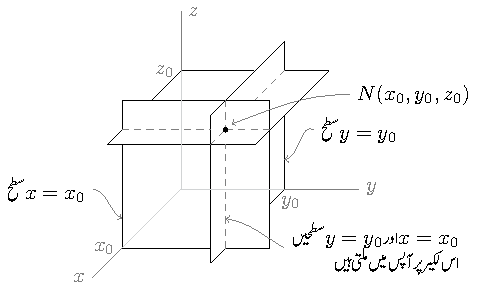
\includegraphics{figLinearAlgebraLineAsSurfacesTouching}
\caption{آپس میں غیر متوازی سطحیں ایک نقطے پر ملتی ہیں}
\label{شکل_خطی_الجبرا_سطح_نقطے_پر_ملتی_ہیں}
\end{figure}
\انتہا{مثال}
%=======================================
مثال \حوالہ{مثال_الجبرا_وجودیت_یکتائی_حل_الف} میں ہم نے دیکھا کہ عین ممکن ہے کہ نظام کا کوئی حل ممکن نہ ہو۔یوں کسی بھی نظام کے بارے میں ہم جاننا چاہیں گے کہ آیا اس کا حل موجود ہے اور آیا ایسا حل یکتا ہے۔آئیں اب خطی نظام کو حل کرنے کا منظم طریقہ سیکھیں۔
%========================

\جزوحصہء{گاوسی اسقاط}
ہم درج ذیل خطی نظام پر غور کرتے ہیں۔
\begin{align*}
2x_1+x_2&=7\\
4x_2&=12
\end{align*}
اس نظام کے عددی سر قالب میں غیر صفر قیمتیں، مرکزی وتر اور اس سے اوپر ہیں لہٰذا یہ \اصطلاح{بالائی تکونی نظام} ہے۔اس نظام کی نچلی مساوات کو حل کرتے ہوئے \عددی{x_2=\tfrac{12}{4}=3} ملتا ہے جس کو پہلی مساوات میں واپس پر کرتے ہوئے \عددی{x_1=\tfrac{7-x_2}{2}=\tfrac{7-3}{2}=2} حاصل ہوتا ہے۔اس عمل سے ہم دیکھتے ہیں کہ تکونی نظام کو با آسانی حل کیا جا سکتا ہے۔یوں ہم  کسی بھی نظام کو تکونی صورت میں لکھنا چاہیں گے۔

کسی بھی نظام کو تکونی صورت میں لانے کے عمل کو درج ذیل نظام کی مدد سے سیکھتے ہیں جس کا افزودہ قالب بھی دیا گیا ہے۔افزودہ قالب کی پہلی صف کو \عددی{S_1} اور دوسری صف کو \عددی{S_2} کہا گیا ہے۔
\begin{gather*}
\begin{matrix} S_1\\S_2 \end{matrix}\begin{bmatrix*}[r]2&3&&12\\ 4&-2&&8  \end{bmatrix*}\quad \quad\quad 
\begin{aligned}
2x_1+3x_2&=12\\
4x_1-2x_2&=8
\end{aligned}
\end{gather*} 
اس کو تکونی صورت میں لکھنے کی خاطر نچلی مساوات سے \عددی{x_1} حذف کرنا ہو گا۔ایسا کرنے کے لئے بالائی مساوات کو \عددی{2} سے ضرب دے کر 
\عددی{4x_1+6x_2=24} حاصل کرتے ہوئے اس کو  نچلی مساوات سے منفی کرتے ہیں جس سے \عددی{-8x_2=-16} ملتا ہے۔یوں درج بالا نظام درج ذیل لکھا جائے گا جو بالائی تکونی صورت ہے۔افزودہ قالب پر بھی یہی عمل کیا گیا ہے جہاں نچلی صف کے  ساتھ الجبرائی عمل \عددی{(S_2-2S_1)} لکھا گیا ہے۔
\begin{gather*}
\begin{bmatrix*}[r] 2&3&&12\\0 &-8&&-16 \end{bmatrix*}\begin{matrix} \\ S_2-2S_1 \end{matrix}\quad \quad
 \begin{aligned}
2x_1+3x_2&=12\\
-8x_2&=-16
\end{aligned} 
\end{gather*} 
تکونی صورت حاصل کرنے کی اس عمل کو \اصطلاح{گاوسی اسقاط}\فرہنگ{گاوسی اسقاط}\حاشیہب{Gaussian elimination}\فرہنگ{Gauss elimination} کہتے ہیں۔گاوسی اسقاط کی ترکیب وسیع تر نظام پر قابل استعمال ہے۔یوں نچلی مساوات سے \عددی{x_2=2} حاصل کرتے ہوئے پہلی مساوات میں واپس پر کرتے ہوئے \عددی{x_1=3} ملتا ہے۔
%=================
\ابتدا{مثال}\شناخت{مثال_الجبرا_گاوسی_اسقاط_الف}\quad گاوسی اسقاط\\
درج ذیل نظام کو گاوسی اسقاط سے بالائی تکونی صورت میں لائیں۔نظام کا افزودہ قالب بھی دیا گیا ہے۔
\begin{gather*}
\begin{bmatrix*}[r]
1&2&-1&&5\\
2&-3&1&&0\\
-1&2&3&&-3
\end{bmatrix*}\quad \quad \quad
\begin{aligned}
x_1+2x_2-x_3&=5\\
2x_1-3x_2+x_3&=0\\
-x_1+2x_2+3x_3&=-3
\end{aligned}
\end{gather*}
حل:بالائی تکونی صورت کے لئے درمیانی مساوات سے \عددی{x_1} حذف کرنا ہو گا جبکہ نچلی مساوات سے \عددی{x_1} اور \عددی{x_2} حذف کرنے ہوں گے۔

پہلی قدم میں ہم بالائی مساوات  کو استعمال کرتے ہوئے نچلی دونوں مساواتوں سے \عددی{x_1} حذف کرتے ہیں۔پہلی مساوات کو \عددی{2} سے ضرب دے کر دوسری مساوات سے منفی کرنے سے دوسری مساوات سے \عددی{x_1} حذف ہو گا۔اسی طرح پہلی مساوات کو تیسری مساوات کے ساتھ جمع کرتے ہوئے تیسری مساوات سے \عددی{x_1} حذف ہوتا ہے۔اس عمل کو افزودہ قالب کے لئے بیان کرتے ہیں۔ہم ہر قدم پر گزشتہ قالب کی پہلی صف کو \عددی{S_1}، دوسری کو \عددی{S_2} اور تیسری کو \عددی{S_3} کہیں گے۔ یوں درج ذیل میں \عددی{S_1} سے مراد درج بالا قالب کی پہلی صف \عددی{\begin{bmatrix}1&2&-1&&5 \end{bmatrix}} ہے۔

 پہلی صف کو \عددی{2} سے ضرب دیتے ہوئے دوسری صف سے منفی کریں یعنی \عددی{S_2-2S_1}\\
پہلی صف کو تیسری صف کے ساتھ جمع کریں یعنی \عددی{S_3+S_1}

ان عمل صف (یعنی \عددی{S_2-2S_1} اور \عددی{S_3+S_1}) کو درج ذیل قالب کے دائیں جانب مطابقتی صف کے سامنے لکھا گیا ہے۔

\begin{gather*}
\begin{bmatrix*}[r] 1&2&-1&&5\\0&-7&3&&-10\\0&4&2&&2  \end{bmatrix*}\begin{matrix*}[l]  \\ S_2-2S_1\\S_3+S_1\end{matrix*}
\begin{aligned}\quad \quad \quad
x_1+2x_2-x_3&=5\\
-7x_2+3x_3&=-10\\
4x_2+2x_3&=2
\end{aligned}
\end{gather*}
صف پر عمل کو الجبرائی صورت میں قالب کے دائیں جانب لکھا گیا ہے جہاں \عددی{S_1}، \عددی{S_2}، \نقطے  گزشتہ قالب کے صف ہیں۔درج بالا تبدیل شدہ افزودہ قالب ہے۔

دوسری قدم میں (درج بالا حاصل کردہ کی) نچلی مساوات سے \عددی{x_2} حذف کرتے ہیں۔

تبدیل شدہ افزودہ قالب کی دوسری صف کو \عددی{\tfrac{4}{7}} سے ضرب دیتے ہوئے اسی قالب کی تیسری صف کے ساتھ جمع \عددی{(S_3+\tfrac{4}{7}S_2)} کریں۔یہاں \عددی{S_2} اور \عددی{S_3} سے مراد درج بالا قالب کی دوسری اور تیسری صف ہے۔یوں \عددی{S_2} سے مراد \عددی{\begin{bmatrix}0&-7&3&&-10  \end{bmatrix}} ہے۔
\begin{gather}\label{مساوات_الجبرا_مثال_گاوسی_اسقاط_الف}
\begin{bmatrix*}[r] 1&2&-1&&5\\0&-7&3&&-10\\0&0&\frac{26}{7}&&-\frac{26}{7}  \end{bmatrix*}\begin{matrix*}[l]  \\ \\S_3+\frac{4}{7}S_2\end{matrix*}\quad \quad\quad
\begin{aligned}
x_1+2x_2-x_3&=5\\
-7x_2+3x_3&=-10\\
\frac{26}{7}x_3&=-\frac{26}{7}
\end{aligned}
\end{gather}
تکونی قالب کے حصول کے بعد حل حاصل کرتے ہیں۔نظام \حوالہ{مساوات_الجبرا_مثال_گاوسی_اسقاط_الف} کی نچلی مساوات سے \عددی{x_3=-1} ملتا ہے جس کو نظام \حوالہ{مساوات_الجبرا_مثال_گاوسی_اسقاط_الف} کی درمیانی مساوات میں واپس پر کرتے ہوئے \عددی{x_2=1} ملتا ہے۔ان دونوں جوابات کو پہلی مساوات میں پر کرتے ہوئے \عددی{x_1=2} ملتا ہے۔

اگر دوسری قدم پر آپ پہلی مساوات کو \عددی{2} سے ضرب دے کر تیسری مساوات سے منفی کریں تو حاصل مساوات میں \عددی{x_1} دوبارہ حاضر ہو جائے گا جو پہلی قدم کی محنت کو ضائع کر دے گا۔ہم ایسا نہیں چاہتے ہیں۔یوں آپ دیکھ سکتے ہیں کہ کسی بھی جسامت کی نظام کو حل کرتے ہوئے  پہلی قدم پر، نظام کی پہلی مساوات کو استعمال کرتے ہوئے، اس سے نیچے تمام مساوات سے \عددی{x_1} حذف کیا جاتا ہے۔ دوسری قدم پر، پہلی قدم کی حاصل نظام کی دوسری مساوات کو استعمال کرتے ہوئے، اس سے نیچے تمام مساواتوں سے \عددی{x_2} حذف کیا جاتا ہے۔اسی طرح تیسری قدم پر، تیسری مساوات کو استعمال کرتے ہوئے، اس سے نیچے تمام مساواتوں سے \عددی{x_3} حذف کیا جائے گا۔یہی سلسلہ آخر تک دہرایا جائے گا۔

اس نظام کو افزودہ قالب استعمال کرتے ہوئے حل کیا جا سکتا تھا۔ بار بار مکمل مساوات لکھنے کی کوئی ضرورت نہیں تھی۔ہم عموماً ایسا ہی کرتے ہوئے ،نظام کو افزودہ قالب کی صورت میں لکھ کر، اس کی تکونی صورت گاوسی اسقاط کی مدد سے حاصل کریں گے۔  
\انتہا{مثال}
%=====================
\ابتدا{مثال}\شناخت{مثال_الجبرا_دور_گاوسی_اسقاط}
برقی دور کو شکل \حوالہ{شکل_مثال_الجبرا_دور_گاوسی_اسقاط} میں دکھایا گیا ہے۔اس کو حل کریں۔
\begin{figure}
\centering
\begin{tikzpicture}
\draw (0,0) to [american voltage source,l={$\SI{10}{\volt}$}]++(0,\y) to [resistor,l={$\SI{2}{\ohm}$},i>^={$I_1$}]++(\x,0) to [resistor,l={$\SI{8}{\ohm}$},i={$I_2$}]++(0,-\y) to [short]++(-\x,0);
\draw(\x,0) to [short,*-]++(\x,0) to [american voltage source,l_={$\SI{8}{\volt}$}]++(0,\y) to [resistor,l_={$\SI{4}{\ohm}$},i>_={$I_3$},-*]++(-\x,0);
\end{tikzpicture}
\caption{برقی دور۔ مثال \حوالہ{مثال_الجبرا_دور_گاوسی_اسقاط}}
\label{شکل_مثال_الجبرا_دور_گاوسی_اسقاط}
\end{figure}
حل:کرخوف قانون دباو سے درج ذیل لکھا جا سکتا ہے
\begin{align*}
2I_1+8I_3&=10\\
4I_3+8I_2&=8
\end{align*}
جبکہ کرخوف قانون رو سے درج ذیل لکھا جا سکتا ہے۔
\begin{align*}
I_1+I_3&=I_2
\end{align*}
ان تینوں مساوات کو ترتیب دیتے ہوئے ایک ساتھ لکھتے ہیں۔ ساتھ ہی بائیں جانب اس نظام کا افزودہ قالب بھی لکھتے ہیں۔
\begin{gather*}
\begin{bmatrix*}[r]2&0&8&&10\\0&8&4&&8\\
1&-1&1&&0  \end{bmatrix*}\quad \quad \quad 
\begin{aligned}
2I_1+8I_3&=10\\
8I_2+4I_3&=8\\
I_1-I_2+I_3&=0
\end{aligned}
\end{gather*}
پہلا قدم: چونکہ دوسری صف کا پہلا رکن صفر ہے لہٰذا اس کو کچھ کرنے کی ضرورت نہیں ہے البتہ تیسرے صف کے پہلے رکن \عددی{I_1} کو حذف کرنا ہو گا۔

پہلی صف کو \عددی{\tfrac{1}{2}} سے ضرب دے کر تیسری صف سے منفی کرتے ہیں۔درج ذیل میں \عددی{S_3} سے مراد درج بالا قالب کی تیسری صف
 \عددی{\begin{bmatrix}1&-1&1&&0  \end{bmatrix}} ہے۔
\begin{gather*}
\begin{bmatrix*}[r]2&0&8&&10\\0&8&4&&8\\
0&-1&-3&&-5  \end{bmatrix*}\begin{matrix} \\ \\ S_3-\frac{1}{2}S_1 \end{matrix} \quad \quad 
\begin{aligned}
2I_1+8I_3&=10\\
8I_2+4I_3&=8\\
-I_2-3I_3&=-5
\end{aligned}
\end{gather*}
دوسرا قدم: درج بالا کے تیسرے صف سے \عددی{I_2} حذف کرتے ہیں۔

دوسرے صف کو \عددی{\tfrac{1}{8}} سے ضرب دے کر تیسرے صف کے ساتھ جمع کرتے ہیں۔ 

درج ذیل لکھتے ہوئے \عددی{S_3} سے مراد گزشتہ (درج بالا) قالب کی تیسری صف \عددی{\begin{bmatrix}0&-1&-3&&-5  \end{bmatrix}} ہے۔
\begin{gather*}
\begin{bmatrix*}[r]2&0&8&&10\\0&8&4&&8\\
0&0&-\frac{5}{2}&&-4  \end{bmatrix*}\begin{matrix} \\ \\ S_3+\frac{1}{8}S_2 \end{matrix} \quad \quad 
\begin{aligned}
2I_1+8I_3&=10\\
8I_2+4I_3&=8\\
-\frac{5}{2}I_3&=-4
\end{aligned}
\end{gather*}
تیسرا قدم: آخری صف یا آخری مساوات سے \عددی{I_3=\tfrac{8}{5}} ملتا ہے۔اس قیمت کو درج بالا پہلی اور  اور درمیانی مساوات  میں پر کرتے ہوئے بقایا برقی رو حاصل کرتے ہیں۔
\begin{align*}
2I_1+8\left(\frac{8}{5}\right)&=10\quad \implies \quad I_1=-\frac{7}{5}\\
8I_2+4\left(\frac{8}{5}\right)&=8\quad \implies \quad I_2=\frac{1}{5}
\end{align*}
\انتہا{مثال}
%==========================================
\ابتدا{مثال}\شناخت{مثال_الجبرا_یکتا_حل_گاوسی_اسقاط}
درج ذیل نظام کو گاوسی اسقاط سے حل کریں۔
\begin{gather*}
\begin{bmatrix*}[r]
2&-1&1&&5\\
1&1&1&&2\\
1&2&-1&&-3\\
1&-1&-1&&0
\end{bmatrix*}\quad\quad\quad \quad
\begin{aligned}
2x_1-x_2+x_3&=5\\
x_1+x_2+x_3&=2\\
x_1+2x_2-x_3&=-3\\
x_1-x_2-x_3&=0
\end{aligned}
\end{gather*}
حل:پہلی قدم میں دوسری، تیسری اور چوتھی صف سے \عددی{x_1} حذف کرتے ہیں۔
\begin{gather*}
\begin{bmatrix*}[r]
2&-1&1&&5\\[0.5ex]
0&\frac{3}{2}&\frac{1}{2}&&-\frac{1}{2}\\[0.5ex]
0&\frac{5}{2}&-\frac{3}{2}&&-\frac{11}{2}\\[0.5ex]
0&-\frac{1}{2}&-\frac{3}{2}&&-\frac{5}{2}
\end{bmatrix*}
\begin{matrix}
\\[0.5ex]
S_2-\frac{1}{2}S_1\\[0.5ex]
S_3-\frac{1}{2}S_1\\[0.5ex]
S_4-\frac{1}{2}S_1\\
\end{matrix}
\quad\quad \quad
\begin{aligned}
2x_1-x_2+x_3&=5\\
\frac{3}{2}x_2+\frac{1}{2}x_3&=-\frac{1}{2}\\
\frac{5}{2}x_2-\frac{3}{2}x_3&=-\frac{11}{2}\\
-\frac{1}{2}x_2-\frac{3}{2}x_3&=-\frac{5}{2}
\end{aligned}
\end{gather*}
دوسری قدم میں تیسری اور چوتھی مساوات سے \عددی{x_2} حذف کرتے ہیں۔
\begin{gather*}
\begin{bmatrix*}[r]
2&-1&1&&5\\[0.5ex]
0&\frac{3}{2}&\frac{1}{2}&&-\frac{1}{2}\\[0.5ex]
0&0&-\frac{7}{3}&&-\frac{14}{3}\\[0.5ex]
0&0&-\frac{4}{3}&&-\frac{8}{3}
\end{bmatrix*}
\begin{matrix}
\\[0.5ex]
\\[0.5ex]
S_3-\frac{5}{3}S_2\\[0.5ex]
S_4+\frac{1}{3}S_2\\
\end{matrix}
\quad\quad \quad
\begin{aligned}
2x_1-x_2+x_3&=5\\
\frac{3}{2}x_2+\frac{1}{2}x_3&=-\frac{1}{2}\\
-\frac{7}{3}x_3&=-\frac{14}{3}\\
-\frac{4}{3}x_3&=-\frac{8}{3}
\end{aligned}
\end{gather*}
ہم تیسرے قدم پر تیسری یا چوتھی مساوات سے \عددی{x_3=2} حاصل کرتے ہیں جس کو دوسری مساوات میں پر کرتے ہوئے \عددی{x_2=-1} ملتا ہے۔انہیں پہلی مساوات میں پر کرتے ہوئے \عددی{x_1=1} ملتا ہے۔
\انتہا{مثال}
%===================================

%===========================================
\جزوحصہء{بنیادی اعمال صف}
قالب کی صفوں پر درج ذیل تین عمل سے نظام تبدیل نہیں ہوتا ہے۔گاوسی اسقاط پہلی دو اعمال سے حاصل ہوتا ہے۔
\begin{itemize}
\item
دو صفوں کا آپس میں تبادلہ
\item
صف کو کسی مستقل قیمت سے ضرب دے کر کسی دوسرے (یا اسی) صف کے ساتھ جمع کرنا
\item
کسی صف کو \موٹا{غیر صفر} مستقل قیمت \عددی{c} کے ساتھ ضرب دینا
\end{itemize} 
دھیان رہے کہ یہ اعمال افزودہ قالب کے صفوں پر قابل اطلاق ہیں نہ کہ قطاروں پر۔یہ اعمال، نظام کی مساوات پر درج ذیل کے مترادف ہیں۔
\begin{itemize}
\item
دو مساواتوں کی جگہ آپس میں تبدیل کرنا۔
\item
ایک مساوات کو کسی مستقل سے ضرب دے کر دوسری (یا اسی) مساوات کے ساتھ جمع کرنا۔
\item
نظام کی مساوات کو \موٹا{غیر صفر} مستقل \عددی{c} سے ضرب دینا۔
\end{itemize}

اب ظاہر ہے کہ ہمزاد مساواتوں کو آگے پیچھے لکھنے سے ان کا حاصل حل تبدیل نہیں ہوتا۔اسی طرح کسی مساوات کو مستقل قیمت سے ضرب دے کر دوسری مساوات کے ساتھ جمع کرنے سے بھی حل تبدیل نہیں ہوتا اور نہ ہی کسی مساوات کو \موٹا{غیر صفر} مستقل سے ضرب دینے سے حل تبدیل ہوتا ہے۔(کسی مساوات کو \موٹا{صفر} سے ضرب دینے سے  مساواتوں کی تعداد کم ہو گی جس سے عین ممکن ہے کہ ان کا حل ممکن نہ رہے۔)

دو عدد خطی نظام \عددی{N_1} اور \عددی{N_2} اس صورت \اصطلاح{صف برابر}\فرہنگ{صف برابر}\حاشیہب{row equivalent}\فرہنگ{row equivalent} کہلاتے ہیں جب \عددی{N_1} پر محدود عمل صف کے ذریعہ \عددی{N_2} حاصل کرنا ممکن ہو۔ یہ حقیقت جسے درج ذیل طور پر بیان کیا جا سکتا ہے، گاوسی اسقاط کی جواز ہے۔
%===========================

\ابتدا{مسئلہ}\quad صف برابر نظام\\
صف برابر خطی نظام کے \اصطلاح{سلسلہ حل}\فرہنگ{سلسلہ!حل}\فرہنگ{حل!سلسلہ}\حاشیہب{solution set}\فرہنگ{solution set} یکساں ہوں گے۔
\انتہا{مسئلہ}
%==========================

اس مسئلے کی بنا اگر ایک نظام کا سلسلہ حل دوسرے نظام کے سلسلہ حل کے عین مطابق ہو، تب انہیں \اصطلاح{صف برابر نظام} کہتے ہیں۔یاد رہے کہ یہاں \اصطلاح{عمل صف} کی بات کی جا رہی ہے۔افزودہ قالب کے قطار تبدیل کرنے سے نظام تبدیل ہو گا اور اس کا حل بھی تبدیل ہو گا لہٰذا افزودہ قالب پر کسی بھی عمل قطار کی اجازت نہیں ہے۔  

ایسا نظام جس کی نا معلوم متغیرات سے مساواتوں کی تعداد زیادہ ہو \اصطلاح{زائد معلوم}\فرہنگ{زائد معلوم}\حاشیہب{overdetermined}\فرہنگ{overdetermined} کہلاتا ہے۔ نظام  کی نا معلوم متغیرات اور مساواتوں کی تعداد برابر ہونے کی صورت میں اس کو \اصطلاح{معلوم}\فرہنگ{معلوم}\حاشیہب{determined}\فرہنگ{determined} کہتے ہیں جبکہ  نظام  کی نا معلوم متغیرات سے مساواتوں کی تعداد کم ہونے کی صورت میں اس کو  \اصطلاح{کم معلوم}\فرہنگ{کم معلوم}\حاشیہب{underdetermined}\فرہنگ{underdetermined} کہتے ہیں۔

ایسا نظام جس کا کوئی حل نہ ہو \اصطلاح{متضاد}\فرہنگ{متضاد}\حاشیہب{inconsistent}\فرہنگ{inconsistent} نظام کہلاتا ہے جبکہ ایسا نظام جس کا ایک یا ایک سے زیادہ حل ممکن ہوں \اصطلاح{بلا تضاد}\فرہنگ{بلا تضاد}\حاشیہب{consistent}\فرہنگ{consistent} نظام کہلاتا ہے۔
%===================

\جزوحصہء{گاوسی اسقاط۔ نظام کی تین ممکنہ صورتیں}
یکتا حل کا نظام مثال \حوالہ{مثال_الجبرا_گاوسی_اسقاط_الف} میں دیکھا گیا۔آئیں اب لامتناہی تعداد کے حل والے نظام (مثال \حوالہ{مثال_الجبرا_لامتناہی_حل_الف}) کو اور بغیر کسی حل والے نظام (مثال \حوالہ{مثال_الجبرا_لامتناہی_حل_ب}) کو گاوسی اسقاط سے حل کرنے کی کوشش کریں۔   

%===================
\ابتدا{مثال}\شناخت{مثال_الجبرا_لامتناہی_حل_الف}\quad لامتناہی تعداد کے حل والا نظام\\
درج ذیل نظام جو تین مساوات پر مبنی ہے میں چار متغیرات پائے جاتے ہیں۔ اس کو گاوسی اسقاط سے حل کریں۔
\begin{gather*}
\begin{bmatrix*}[r]2&1&2&-1&&6\\4&-2&1&2&&2\\8&-4&2&4&&4  \end{bmatrix*}\quad\quad \quad
\begin{aligned}
2x_1+x_2+2x_3-x_4&=6\\
4x_1-2x_2+x_3+2x_4&=2\\
8x_1-4x_2+2x_3+4x_4&=4
\end{aligned}
\end{gather*}
حل:پہلی قدم میں نچلی دو مساواتوں سے \عددی{x_1} حذف کرتے ہیں۔

پہلی صف کو \عددی{2} سے ضرب کرتے ہوئے دوسری صف سے منفی \عددی{(S_2-2S_1)} کریں۔\\
پہلی صف کو \عددی{4} سے ضرب کرتے ہوئے تیسری صف سے منفی \عددی{(S_3-4S_1)} کریں۔
\begin{gather*}
\begin{bmatrix*}[r]2&1&2&-1&&6\\0&-4&-3&4&&-10 \\0&-8&-6&8&&-20\end{bmatrix*}\begin{matrix*}[r]  \\S_2-2S_1\\S_3-4S_1  \end{matrix*}\quad\quad \quad
\begin{aligned}
2x_1+x_2+2x_3-x_4&=6\\
-4x_2-3x_3+4x_4&=-10\\
-8x_2-6x_3+8x_4&=-20
\end{aligned}
\end{gather*}
دوسری قدم میں درج بالا تبدیل شدہ افزودہ قالب استعمال کرتے ہوئے، دوسرے صف کی مدد سے تیسری صف سے \عددی{x_2} حذف کرتے ہیں۔دوسری صف کو دو سے ضرب دیتے ہوئے تیسری صف سے منفی کرتے ہیں۔
\begin{gather*}
\begin{bmatrix*}[r]2&1&2&-1&&6\\0&-4&-3&4&&-10 \\0&0&0&0&&0\end{bmatrix*}\begin{matrix*}[r]  \\\\S_3-2S_2  \end{matrix*}\quad\quad \quad
\begin{aligned}
2x_1+x_2+2x_3-x_4&=6\\
-4x_2-3x_3+4x_4&=-10\\
0&=0
\end{aligned}
\end{gather*}
دوسری مساوات سے \عددی{x_2=\tfrac{5}{2}-\tfrac{3}{4}x_3+x_4} اور یوں پہلی مساوات سے \عددی{x_1=\tfrac{7}{4}-\tfrac{5}{8}x_3} ملتا  ہے۔اب \عددی{x_3} اور \عددی{x_4} کی لامحدود مختلف قیمتیں پر کرتے ہوئے \عددی{x_1} اور \عددی{x_2} حاصل کیے جا سکتے ہیں۔

عموماً اختیاری مستقل کو \عددی{t_1}، \عددی{t_2}، \نقطے لکھا جاتا ہے۔یوں \عددی{x_3} اور \عددی{x_4} کو بالترتیب \عددی{t_1} اور \عددی{t_2} لکھتے ہوئے درج ذیل لکھا جائے گا۔
\begin{align*}
x_1&=\tfrac{7}{4}-\tfrac{5}{8}t_1\\
x_2&=\tfrac{5}{2}-\tfrac{3}{4}t_1+t_2
\end{align*}
\انتہا{مثال}
%========================
\ابتدا{مثال}\شناخت{مثال_الجبرا_لامتناہی_حل_ب}\quad گاوسی اسقاط۔بلا حل نظام\\
ایسا نظام جس کا حل ممکن نہ ہو کو گاوسی اسقاط سے حل کرتے ہوئے \ترچھا{تضاد} کی صورت حاصل ہو گی۔آئیں درج ذیل نظام حل کرنے کی کوشش کرتے ہیں۔
\begin{gather*}
\begin{bmatrix*}[r] 4&-2&2&&6\\2&4&-2&&6\\-2&16&-10&&14  \end{bmatrix*}\quad \quad \quad 
\begin{aligned}
4x_1-2x_2+2x_3&=6\\
2x_1+4x_2-2x_3&=6\\
-2x_1+16x_2-10x_3&=14
\end{aligned}
\end{gather*}
دوسری اور تیسری مساوات سے \عددی{x_1} حذف کرتے ہیں۔

پہلی صف کو \عددی{\tfrac{1}{2}} سے ضرب دے کر دوسری صف سے منفی کرتے ہیں۔\\
پہلی صف کو \عددی{\tfrac{1}{2}} سے ضرب دے کر تیسری صف کے ساتھ جمع کرتے ہیں۔
\begin{gather*}
\begin{bmatrix*}[r] 4&-2&2&&6\\0&5&-3&&3\\0&15&-9&&17  \end{bmatrix*}\begin{matrix}\\S_2-\frac{1}{2}S_1\\S_3+\frac{1}{2}S_1  \end{matrix}\quad \quad \quad 
\begin{aligned}
4x_1-2x_2+2x_3&=6\\
5x_2-3x_3&=3\\
15x_2-9x_3&=17
\end{aligned}
\end{gather*}
آخری صف سے \عددی{x_2} حذف کرتے ہیں۔
\begin{gather*}
\begin{bmatrix*}[r] 4&-2&2&&6\\0&5&-3&&3\\0&0&0&&8  \end{bmatrix*}\begin{matrix}\\\\S_3-3S_2  \end{matrix}\quad \quad \quad 
\begin{aligned}
4x_1-2x_2+2x_3&=6\\
5x_2-3x_3&=3\\
0&=8
\end{aligned}
\end{gather*}
آخری مساوات کے تحت \عددی{0=8} ہے جو \ترچھا{تضاد} کی صورت ہے۔بلا حل نظام کی گاوسی اسقاط \ترچھا{تضاد} کی صورت دے گی۔
\انتہا{مثال}
%========================

\جزوحصہ{صف زینہ دار صورت}
گاوسی اسقاط کے بعد حاصل عددی سر قالب، افزودہ قالب اور نظام  \اصطلاح{صف زینہ دار}\فرہنگ{صف زینہ دار}\حاشیہب{echelon form}\فرہنگ{echelon form} کہلاتے ہیں جن میں صفر کے صف، اگر موجود ہوں تو یہ،  آخر پر پائے جاتے ہیں اور صف میں بائیں جانب پہلی غیر صفر اندراج، ہر اگلے صف میں، مزید دور ہو گی۔ مثال \حوالہ{مثال_الجبرا_لامتناہی_حل_ب} میں عددی سر قالب اور افزودہ قالب کی زینہ دار صورت درج ذیل ہیں۔
\begin{align*}
\begin{bmatrix*}[r] 3&2&1&&3\\0&-\frac{1}{3}&\frac{1}{3}&&-2\\0&0&0&&12  \end{bmatrix*} \quad \quad \begin{bmatrix*}[r] 3&2&1\\0&-\frac{1}{3}&\frac{1}{3}\\0&0&0 \end{bmatrix*}
\end{align*}
دھیان رہے کہ ہم بائیں ترین اندراج کو اکائی \عددی{(1)} کی صورت میں لانے کی کوشش نہیں کرتے ہیں چونکہ اس سے کوئی فائدہ حاصل نہیں ہو گا۔  (\اصطلاح{سادہ زینہ دار صورت}\فرہنگ{زینہ دار صورت!سادہ}\حاشیہب{reduced echelon form}\فرہنگ{echelon form!reduced} جس میں بائیں ترین اندراج اکائی ہو گی پر بعد میں بحث کی جائے گی۔)

\عددی{m} مساوات اور \عددی{n} متغیرات کے نظام کا افزودہ قالب \عددی{\begin{bmatrix}\bM{A}\,|\, \bM{b}  \end{bmatrix}} ہے جس سے  زینہ دار صورت
 \عددی{\begin{bmatrix}\bM{R}\,|\,\bM{f}  \end{bmatrix}} حاصل کی جاتی ہے۔ نظام \عددی{\bM{a}\bM{x}=\bM{b}} اور \عددی{\bM{R}\bM{x}=\bM{f}} ایک ہی نظام کو لکھنے کے دو طریقے ہیں۔اگر ان میں کسی ایک نظام کا حل موجود ہو، تب یہی حل دوسرے نظام کا  بھی حل ہو گا۔

گاوسی اسقاط سے  \ترچھا{زینہ دار افزودہ قالب} کی درج ذیل عمومی صورت حاصل ہو گی۔
\begin{align*}
\begin{bmatrix}
r_{11}&r_{12}&r_{13}&\cdots&\cdots&r_{1n}&&f_1\\
0&r_{22}&r_{23}&\cdots&\cdots&r_{2n}&&f_2\\
\vdots\\
0&0&\cdots&r_{rr}&\cdots&r_{rn}&&f_r\\
0&0&0&\cdots&\cdots&0&&f_{r+1}\\
\vdots\\
0&0&0&\cdots&\cdots&0&&f_m
\end{bmatrix}
\end{align*} 
درج بالا زینہ دار افزودہ قالب میں \عددی{r \le m}، \عددی{r_{rr} \ne 0}  جبکہ  \عددی{f_{r+1}} تا \عددی{f_m} اندراج والے صف میں تمام \عددی{r_{ij}=0} ہوں گے۔

\ترچھا{زینہ دار عددی سر قالب} \عددی{\bM{R}} میں غیر صفر صفوں کی تعداد \عددی{r} کو \عددی{\bM{A}} کا \اصطلاح{درجہ}\فرہنگ{درجہ قالب}\حاشیہب{rank of matrix}\فرہنگ{rank} کہتے ہیں جو \عددی{\bM{A}} کا بھی \اصطلاح{درجہ} ہو گا۔یہ جاننا کہ نظام \عددی{\bM{A}\bM{x}=\bM{b}} کا حل موجود ہے یا نہیں اور اس حل کو حاصل کرنا درج ذیل طریقے سے ممکن ہے۔
%====================
\begin{itemize}
\item{(الف) بلا حل:}
اگر \عددی{r<m} ہو (جس کا مطلب ہے کہ \عددی{\bM{R}} میں کم از کم ایک صف ایسا ہے جس کے تمام اندراجات صفر \عددی{(0)} ہیں) اور \عددی{f_{r+1}} تا \عددی{f_m} میں سے کم از کم ایک مقدار غیر صفر ہو تب \عددی{\bM{R}\bM{x}=\bM{f}} \اصطلاح{متضاد} نظام ہو گا جس کا کوئی حل ممکن نہیں ہے۔یوں \عددی{\bM{A}\bM{x}=\bM{b}} بھی \ترچھا{متضاد} نظام ہو گا جس کا کوئی حل نہیں پایا جاتا ہے۔ 
\end{itemize}
\اصطلاح{بلا تضاد} نظام (جس میں یا \عددی{r= m} ہو اور یا \عددی{r<m} کے ساتھ ساتھ \عددی{f_{r+1}} تا \عددی{f_m} صفر کے برابر ہوں) تب نظام کا حل درج ذیل ہو گا۔
\begin{itemize}
\item{(ب) یکتا حل:}
اگر \عددی{r=n} ہو تب نظام کا حل یکتا ہو گا جس کو گاوسی اسقاط سے حاصل کیا جا سکتا ہے۔(مثال \حوالہ{مثال_الجبرا_گاوسی_اسقاط_الف} کی طرح۔) 
\item{(پ) بے انتہا تعداد کے حل:}
ایسی صورت میں \عددی{x_{r+1}} تا \عددی{x_n} کی  قیمتیں چن کر \عددی{x_1} تا \عددی{x_{r-1}} حاصل کریں۔(مثال \حوالہ{مثال_الجبرا_لامتناہی_حل_الف} کی طرح۔)
\end{itemize}
%================================

\حصہء{سوالات}
سوال \حوالہ{سوال_الجبرا_گاوسی_اسقاط_الف} تا سوال \حوالہ{سوال_الجبرا_گاوسی_اسقاط_ب} کو گاوسی اسقاط سے حل کریں۔

%================
\ابتدا{سوال}\شناخت{سوال_الجبرا_گاوسی_اسقاط_الف}
\begin{align*}
2x-3y&=-4\\
x+y&=3
\end{align*}
جوابات:\عددی{x=1,\, y=2}
\انتہا{سوال}
%============================
\ابتدا{سوال}
\begin{align*}
\begin{bmatrix*}[r] 1&-2&&-3\\2&1&&-1 \end{bmatrix*}
\end{align*}
جوابات:\عددی{x_1=-1,\,x_2=1}
\انتہا{سوال}
%=============================
\ابتدا{سوال}
\begin{align*}
x-2y+z&=-1\\
y-z&=-1\\
2x+y+z&=1
\end{align*}
جوابات:\عددی{x=-1,\, y=1,\,z=2}
\انتہا{سوال}
%============================
\ابتدا{سوال}
\begin{align*}
\begin{bmatrix*}[r]
1&2&-1&&-2\\0&2&1&&-1\\2&-1&2&&5
\end{bmatrix*}
\end{align*}
جوابات:\عددی{x_1=1,\,x_2=-1,\,x_3=1}
\انتہا{سوال}
%=============================
\ابتدا{سوال}
\begin{align*}
\begin{bmatrix*}[r] 
3&-2&&4\\
2&-1&&3\\
1&1&&3
\end{bmatrix*}
\end{align*}
جوابات:\عددی{x_1=2,\,x_2=1}
\انتہا{سوال}
%===================
\ابتدا{سوال}
\begin{align*}
\begin{bmatrix*}[r]  
4&-8&3&&16\\
-1&2&-5&&-21\\
3&-6&1&&7
\end{bmatrix*}
\end{align*}
جوابات:\عددی{x_3=4,\, x_2=t,\, x_1=2t+1} جہاں \عددی{t} اختیاری مستقل ہے۔
\انتہا{سوال}
%===========================
\ابتدا{سوال}
\begin{align*}
\begin{bmatrix*}[r]
2&4&1&&0\\
-1&1&-2&&0\\
4&0&6&&0
\end{bmatrix*}
\end{align*}
جوابات:\عددی{x_3=t,\, x_2=\tfrac{t}{2},\,x_1=-\tfrac{3}{2}t}  جہاں \عددی{t} اختیاری مستقل ہے۔
\انتہا{سوال}
%============================
\ابتدا{سوال}
\begin{align*}
x-y&=1\\
y+z&=-1\\
2x-y&=6
\end{align*}
جوابات:\عددی{x=2,\, y=-2,\,z=1}
\انتہا{سوال}
%============================
\ابتدا{سوال}
\begin{align*}
2x+y-3z&=-1\\
x+y+z&=1
\end{align*}
جوابات:\عددی{z=t,y=3-5t,x=4t-2}  جہاں \عددی{t} اختیاری مستقل ہے۔
\انتہا{سوال}
%=========================
\ابتدا{سوال}
\begin{align*}
\begin{bmatrix*}[r]
1&2&3&&1\\
1&-1&-1&&3
\end{bmatrix*}
\end{align*}
جوابات:\عددی{x=\tfrac{1}{3}(7-t), \, y=-\tfrac{1}{3}(4t+2),\, z=t}  جہاں \عددی{t} اختیاری ہے۔ 
\انتہا{سوال}
%===========================
\ابتدا{سوال}
\begin{align*}
\begin{bmatrix*}[r]
1&-1&2&3&&0\\
2&1&-1&1&&0\\
1&1&1&1&&0
\end{bmatrix*}
\end{align*}
جوابات:\عددی{x_4=t,\, x_3=-\tfrac{4}{7}t,\, x_2=\tfrac{5}{7}t,\, x_1=-\tfrac{8}{7}t}  جہاں \عددی{t} اختیاری مستقل ہے۔
\انتہا{سوال}
%===========================
\ابتدا{سوال}
\begin{align*}
\begin{bmatrix*}[r]
0&1&-2&-3&&6\\
2&1&-1&1&&1\\
1&-1&-1&1&&-1
\end{bmatrix*}
\end{align*}
جوابات:\عددی{x_1=-\tfrac{10}{7}(t+1),\, x_2=\tfrac{1}{7}(5t+12),\, x_3=-\tfrac{1}{7}(8t+15)}  جہاں \عددی{t} اختیاری مستقل ہے۔بالائی صف کی جگہ تبدیل کرتے ہوئے حل کریں اور یا نچلی تکونی صورت حاصل کرتے ہوئے حل کریں۔
\انتہا{سوال}
%======================================
\ابتدا{سوال}
\begin{align*}
3x_1+x_2-2x_3-3x_4&=7\\
2x_1+x_2-x_3+x_4&=0\\
x_1-x_2-x_3+x_4&=-5\\
x_1+x_2+x_3-x_4&=7
\end{align*}
جوابات:\عددی{x_1=1,\,x_2=x_3=2,\,x_4=-2}
\انتہا{سوال}
%===================================
\ابتدا{سوال}\شناخت{سوال_الجبرا_گاوسی_اسقاط_ب}
\begin{align*}
\begin{bmatrix*}[r]
1&2&1&-2&&-1\\
2&2&1&1&&4\\
3&-6&-4&6&&16\\
1&1&1&-4&&-3
\end{bmatrix*}
\end{align*}
جوابات:\عددی{x_1=2,\,x_2=0,\,x_3=-1,\,x_4=1}
\انتہا{سوال}
%================================
سوال \حوالہ{سوال_الجبرا_نمونہ_نظام_الف} تا سوال \حوالہ{سوال_الجبرا_نمونہ_نظام_ب} برقی ادوار کے نظام ہیں۔

%======================
\ابتدا{سوال}\شناخت{سوال_الجبرا_نمونہ_نظام_الف}
شکل \حوالہ{شکل_سوال_الجبرا_نمونہ_نظام_الف}-الف میں برقی دور دکھایا گیا ہے۔اس کو حل کریں۔
\begin{figure}
\centering
\begin{subfigure}{0.5\textwidth}
\centering
\begin{tikzpicture}
\draw(0,0) to [american voltage source,l={$\SI{2}{\volt}$}]++(0,\y) to [resistor,l={$\SI{4}{\ohm}$},i={$I_1$}]++(0,\y) to [resistor,l={$\SI{2}{\ohm}$}]++(\x,0) to [resistor,l={$\SI{7}{\ohm}$}]++(\x,0) to [resistor,l={$\SI{1}{\ohm}$},i>^={$I_3$}]++(0,-\y) to [american voltage source,l={$\SI{6}{\volt}$}]++(0,-\y) to [short]++(-2*\x,0);
\draw(\x,0) to [american voltage source,l={$\SI{4}{\volt}$},i={$I_2$},*-]++(0,\y) to [resistor,l={$\SI{6}{\ohm}$},-*]++(0,\y);
\end{tikzpicture}
\caption*{(الف)}
\end{subfigure}%
\begin{subfigure}{0.5\textwidth}
\centering
\begin{tikzpicture}
\draw(0,0) to [american voltage source,l={$\SI{20}{\volt}$}]++(0,\y) to [resistor,l_={$\SI{4}{\ohm}$},i_>={$I_2$}]++(-\x,0) to [resistor,l_={$\SI{16}{\ohm}$},i={$I_4$}]++(0,-\y) to [short,-*]++(\x,0);
\draw(0,\y) to [resistor,*-,l={$\SI{6}{\ohm}$},i={$I_3$}]++(\x,0) to [resistor,l_={$\SI{12}{\ohm}$},i={$I_5$}]++(0,-\y) to [short]++(-\x,0);
\draw(-\x,\y) to [short,*-]++(0,\y/2) to [resistor,l={$\SI{8}{\ohm}$},i={$I_1$}]++(2*\x,0) to [short,-*]++(0,-\y/2);
\end{tikzpicture}
\caption*{(ب)}
\end{subfigure}%
\caption{برقی دور۔ سوال \حوالہ{سوال_الجبرا_نمونہ_نظام_الف} اور سوال \حوالہ{سوال_الجبرا_دور_دوسرا_الف}}
\label{شکل_سوال_الجبرا_نمونہ_نظام_الف}
\end{figure}

جوابات: \عددی{I_1=\tfrac{8}{33}\,\si{\ampere}}،  \عددی{I_2=\tfrac{19}{33}\,\si{\ampere}}،  \عددی{I_3=\tfrac{9}{11}\,\si{\ampere}}
\انتہا{سوال}
%========================
\ابتدا{سوال}\شناخت{سوال_الجبرا_دور_دوسرا_الف}
شکل \حوالہ{شکل_سوال_الجبرا_نمونہ_نظام_الف}-ب میں دکھائے گئے دور کو حل کریں۔


جوابات:\عددی{I_1=\tfrac{10}{57}\,\si{\ampere}}، \عددی{I_2=\tfrac{65}{57}\,\si{\ampere}}، \عددی{I_3=\tfrac{170}{171}\,\si{\ampere}}، \عددی{I_4=\tfrac{55}{57}\,\si{\ampere}}، \عددی{I_5=\tfrac{200}{171}\,\si{\ampere}}
\انتہا{سوال}
%=======================
\ابتدا{سوال}\شناخت{سوال_الجبرا_تقسیم_رو}
شکل \حوالہ{شکل_سوال_الجبرا_تقسیم_رو}-الف میں تینوں برقی رو دریافت کریں۔برقی  رو \عددی{I_2} کی قیمت منفی ہے۔اس کا کیا مطلب ہے؟
\begin{figure}
\centering
\begin{subfigure}{0.5\textwidth}
\centering
\begin{tikzpicture}
\draw(0,0) to [american voltage source,l={$\SI{20}{\volt}$}]++(0,\y) to [resistor,l={$\SI{2}{\ohm}$},i={$I_3$}]++(\x,0) to [short]++(\x,0) to [resistor,l={$\SI{6}{\ohm}$},i<_={$I_2$}]++(0,-\y) to [short]++(-2*\x,0);
\draw(\x,0) to [resistor,*-*,l={$\SI{4}{\ohm}$},i<_={$I_1$}]++(0,\y);
\end{tikzpicture}
\caption*{(الف)}
\end{subfigure}%
\begin{subfigure}{0.5\textwidth}
\centering
\begin{tikzpicture}[american voltages]
\draw(0,0) to [american voltage source,l={$V_s$}]++(0,\y) to [resistor,l={$R_1$},i={$I$}]++(\x,0) to [resistor,l={$R_2$},v={$V_2$}]++(0,-\y) to [short]++(-\x,0);
\end{tikzpicture}
\caption*{(ب) تقسیم دباو کا دور۔}
\end{subfigure}%
\caption{ادوار برائے سوال \حوالہ{سوال_الجبرا_تقسیم_رو} اور سوال \حوالہ{سوال_الجبرا_تقسیم_دباو}}
\label{شکل_سوال_الجبرا_تقسیم_رو}
\end{figure}
جوابات:\عددی{I_1=\tfrac{30}{11}\,\si{\ampere}}، \عددی{I_2=-\tfrac{20}{11}\,\si{\ampere}}، \عددی{I_3=\tfrac{50}{11}\,\si{\ampere}} منفی برقی رو کا مطلب ہے کہ رو کی سمت دکھائی گئی سمت کے الٹ ہے۔
\انتہا{سوال}
%=======================
\ابتدا{سوال}\شناخت{سوال_الجبرا_تقسیم_دباو}
تقسیم دباو کا دور شکل \حوالہ{شکل_سوال_الجبرا_تقسیم_رو}-ب میں دکھایا گیا ہے۔ کرخوف قانون دباو سے \عددی{V_s}، \عددی{I}، \عددی{R_1} اور \عددی{R_2} کا تعلق لکھیں۔اسی طرح \عددی{V_2} اور \عددی{I} کا تعلق لکھیں۔اس نظام کو حل کرتے ہوئے \عددی{V_2} حاصل کریں۔حاصل کلیہ \اصطلاح{تقسیم دباو}\فرہنگ{کلیہ!تقسیم دباو}\فرہنگ{تقسیم دباو!کلیہ}\حاشیہب{voltage division formula}\فرہنگ{voltage division} کا کلیہ کہلاتا ہے۔
جواب:\عددی{V_2=\left(\tfrac{R_2}{R_1+R_2}\right)V_s}
\انتہا{سوال}
%===========================
\ابتدا{سوال}\شناخت{سوال_الجبرا_نمونہ_نظام_ب}\quad ویٹ سٹون پل\\
مزاحمتوں کی پیمائش کے لئے استعمال ہونے والا\حاشیہد{برطانوی سائنسدان چارلس ویٹ سٹون [1802-1875] سے اس دور کا نام منسوب ہے۔} \اصطلاح{ویٹ سٹون پل}\فرہنگ{ویٹ سٹون پل}\حاشیہب{wheatstone bridge}\فرہنگ{wheatstone bridge} شکل میں دکھایا گیا ہے۔ ایک ہاتھ  \عددی{R_1} اور \عددی{R_x} نسب ہیں اور دوسرے ہاتھ \عددی{R_2} اور \عددی{R_3} نسب ہیں۔ دونوں ہاتھ آپس میں متوازی جڑے ہیں۔ایک ہاتھ کے درمیانے نقطے سے دوسرے ہاتھ کے درمیانے نقطے تک \اصطلاح{ایمپیئر پیما}\فرہنگ{ایمپیئر پیما}\حاشیہب{ammeter}\فرہنگ{ammeter}  بطور \موٹا{پُل}\حاشیہب{bridge} نسب کیا گیا ہے جس کی مزاحمت \عددی{R_0} ہے۔ویٹ سٹون پل سے نا معلوم مزاحمت \عددی{R_x} ناپی جاتی ہے۔ متغیر مزاحمت \عددی{R_3} کو تبدیل کیا جاتا ہے حتٰی کہ  ایمپیئر پیما \عددی{I_0=0} ناپے۔اس حالت میں ثابت کریں کہ \عددی{R_x=\tfrac{R_1R_3}{R_2}} ہو گا۔  
\begin{figure}
\centering
\begin{tikzpicture}
\pgfmathsetmacro{\kL}{\xx*cos(45)};
\draw(0,0) to [resistor,l={$R_x$}]++(-\kL,\kL)coordinate(mL) to [resistor,l={$R_1$},-*]++(\kL,\kL)coordinate(T) to [resistor,l={$R_2$}]++(\kL,-\kL)coordinate(mR) to [resistor,l={$R_3$}]++(-\kL,-\kL);
\draw(mL) to [european resistor,*-*,l={$R_0$}] (mR);
\draw(0,0) to [short,*-]++(-1.25*\xx,0) to [american voltage source,l={$V_s$}]++(0,1.25*\yy) |-(T);
\end{tikzpicture}
\caption{ویٹ سٹون پل۔ سوال \حوالہ{سوال_الجبرا_نمونہ_نظام_ب}}
\label{شکل_سوال_الجبرا_ویٹ_سٹون_پل}
\end{figure}
جواب:ایمپیئر پیما اس صورت صفر برقی رو ناپے گی جب \عددی{R_0} کے دونوں اطراف برقی دباو کی قیمت عین برابر ہو۔اگر \عددی{R_0} میں برقی رو صفر کے برابر ہو تب \عددی{R_0} کو دور سے ہٹانے سے دور پر کوئی اثر نہیں ہو گا۔ہم ایسا ہی کرتے ہوئے \عددی{R_0} کو ہٹاتے ہوئے حل کرتے ہیں۔سوال \حوالہ{سوال_الجبرا_تقسیم_دباو} کے تحت \عددی{R_x} پر دباو \عددی{V_x=\left(\tfrac{R_x}{R_1+R_x}\right)V_s} اور \عددی{R_3} پر دباو \عددی{V_3=\left(\tfrac{R_3}{R_2+R_3}\right)V_s} ہو گا۔چونکہ یہ دونوں دباو برابر ہیں لہٰذا \عددی{\left(\tfrac{R_x}{R_1+R_x}\right)V_s=\left(\tfrac{R_3}{R_2+R_3}\right)V_s} ہو گا جس سے درکار جواب حاصل ہوتا ہے۔
\انتہا{سوال}
%======================
\ابتدا{سوال}\شناخت{سوال_الجبرا_آمدورفت}\quad آمد و رفت\\
برقی ادوار حل کرنے کے طریقے دیگر شعبوں میں بھی استعمال کیے جا سکتے ہیں۔شکل \حوالہ{شکل_سوال_الجبرا_آمدورفت} میں شہر کی سڑکوں پر فی گھنٹہ گاڑیوں کی آمد و رفت دکھائی گئی ہے۔کرخوف قانون رو کی مماثل استعمال کرتے ہوئے فی گھنٹہ نا معلوم آمد و رفت \عددی{x_1} تا \عددی{x_4} حاصل کریں۔ کیا حل یکتا حل ہے؟ 
\begin{figure}
\centering
\begin{tikzpicture}
\draw(0,0) to [short,-*,i={$150$}]++(\x,0) to [short,-*,i={$x_4$}]++(\x,0) to [short,i={$100$}]++(\x,0);
\draw(0,\y) to [short,-*,i={$300$}]++(\x,0) to [short,-*,i<={$x_1$}]++(\x,0) to [short,i={$50$}]++(\x,0);
\draw(\x,-\y) to [short,i={$50$}]++(0,\y) to [short,i<={$x_2$}]++(0,\y) to [short,i={$200$}]++(0,\y);
\draw(2*\x,-\y) to [short,i<={$50$}]++(0,\y) to [short,i<={$x_3$}]++(0,\y) to [short,i={$100$}]++(0,\y);
\end{tikzpicture}
\caption{آمد و رفت۔ سوال \حوالہ{سوال_الجبرا_آمدورفت}}
\label{شکل_سوال_الجبرا_آمدورفت}
\end{figure}
جوابات:\عددی{x_2=x_1+100}، \عددی{x_3=-x_1-150} اور \عددی{x_4=x_1+300}؛ حل یکتا نہیں ہے۔
\انتہا{سوال}
%=========================
\ابتدا{سوال}\quad منڈی کی رسد و طلب\\
اشیاء کی مانگ، قیمت اور دستیابی  کو بالترتیب \عددی{M}، \عددی{Q} اور \عددی{D} سے ظاہر کرتے ہیں۔دو شہروں میں رسد و طلبی کی متوازن مساوات
 \عددی{(M_1=D_1,\, M_2=D_2)} کا حل درج ذیل خطی تعلقات سے حاصل کریں، جہاں زیر نوشت میں \عددی{1} پہلے شہر اور \عددی{2} دوسرے شہر کو ظاہر کرتے ہیں۔
\begin{align*}
M_1&=30-3Q_1-2Q_2,\quad D_1=5Q_1-2Q_2+6\\
M_2&=4Q_1-Q_2+10,\quad D_2=3Q_2-6
\end{align*}
جوابات:\عددی{M_1=D_1=7}، \عددی{M_2=D_2=15}، \عددی{Q_1=3}، \عددی{Q_2=7} 
\انتہا{سوال}
%========================
\ابتدا{سوال}\quad ضیائی تالیف\\
روشنی کی توانائی استعمال کرتے ہوئے پودے، پانی \عددی{\ce{H2O}} اور کاربن ڈائی آکسائڈ \عددی{\ce{CO2}} سے آکسیجن \عددی{\ce{O2}} اور گلوکوز \عددی{\ce{C6H12O6}} حاصل کرتے ہیں۔  یہ عمل، جسے درج ذیل کیمیائی مساوات میں پیش کیا گیا ہے، \اصطلاح{ضیائی تالیف}\فرہنگ{ضیائی تالیف}\حاشیہب{photosynthesis}\فرہنگ{photosynthesis} کہلاتی ہے۔
\begin{align*}
x_1\ce{CO2}+x_2\ce{H2O}\ce{->[\text{شعاع}]} x_3\ce{C6H12O6}+x_4\ce{O2}
\end{align*}
کیمیائی مساوات متوازن کرنے سے مراد \عددی{x_1}، \عددی{x_2}، \نقطے کی ایسی کمتر قیمتیں دریافت کرنا ہے کہ مساوات کے بائیں ہاتھ ہر قسم کی ایٹم کی تعداد دائیں ہاتھ اسی ایٹم کی تعداد کے برابر ہو۔ضیائی تالیف کی مساوات کو متوازن کریں۔

جوابات:\عددی{x_1=6}، \عددی{x_2=6}، \عددی{x_3=1}، \عددی{x_4=6}
\انتہا{سوال}
%==========================

\حصہ{خطی غیر تابعیت۔ درجہ قالب۔ سمتی فضا}\شناخت{حصہ_الجبرا_تابعیت_غیر_تابعیت}
ہم خطی نظام کے خصوصیات کو مکمل طور پر حل کی موجودگی اور یکتائی کی نقطہ نظر سے دیکھنا چاہتے ہیں۔ ایسا کرنے کی خاطر ہم خطی الجبرا کے نئے اور  بنیادی تصورات متعارف کرتے ہیں۔ ان میں \اصطلاح{خطی غیر تابعیت} اور \اصطلاح{درجہ قالب} زیادہ اہم ہیں۔ یاد رہے کہ گاوسی اسقاط انہیں پر منحصر ہے۔ 

%==========
\جزوحصہء{سمتیات کی خطی تابعیت اور غیر تابعیت}
\عددی{m} عدد سمتیات \عددی{\bM{a}_{(1)}}، \نقطے، \عددی{\bM{a}_{(m)}} (جن میں ارکان کی تعداد یکساں ہے) کی \اصطلاح{خطی مجموعہ}\فرہنگ{خطی مجموعہ}\حاشیہب{linear combination}\فرہنگ{linear combination} درج ذیل مساوات دیتی ہے،
\begin{align*}
c_1\bM{a}_{(1)}+c_2\bM{a}_{(2)}+\cdots+c_m\bM{a}_{(m)}
\end{align*}
جہاں \عددی{c_1} تا \عددی{c_m} غیر سمتی قیمتیں ہیں۔اب درج ذیل مساوات پر غور کریں۔
\begin{align}\label{مساوات_الجبرا_خطی_غیر_تابعیت_الف}
c_1\bM{a}_{(1)}+c_2\bM{a}_{(2)}+\cdots+c_m\bM{a}_{(m)}=\bM{0}
\end{align}
ظاہر ہے کہ تمام \عددی{c_j} کی قیمت صفر ہونے کی صورت میں مساوات \حوالہ{مساوات_الجبرا_خطی_غیر_تابعیت_الف} درست ہو گا چونکہ ایسی صورت میں \عددی{\bM{0}=\bM{0}} حاصل ہوتا ہے۔ اگر \عددی{m} عدد \عددی{c_j} کی یہ واحد قیمت ہو جس کے لئے مساوات \حوالہ{مساوات_الجبرا_خطی_غیر_تابعیت_الف} درست ہو تب \عددی{\bM{a}_{(1)}} تا \عددی{\bM{a}_{(m)}} سمتیات \اصطلاح{خطی طور غیر تابع}\فرہنگ{خطی طور غیر تابع}\حاشیہب{linear independent}\فرہنگ{linear independent} کہلاتے ہیں اور ہم کہتے ہیں کہ  \عددی{\bM{a}_{(1)}} تا \عددی{\bM{a}_{(m)}} سمتیات کا \اصطلاح{خطی طور غیر تابع  سلسلہ}\فرہنگ{خطی طور غیر تابع سلسلہ}\حاشیہب{linearly independent set}\فرہنگ{linearly independent set} ہے۔اس کے برعکس اگر کسی ایک یا ایک سے زیادہ \عددی{c_j} کی قیمت غیر صفر ہونے کی صورت میں بھی مساوات \حوالہ{مساوات_الجبرا_خطی_غیر_تابعیت_الف} درست ہو تب \عددی{\bM{a}_{(1)}} تا \عددی{\bM{a}_{(m)}} سمتیات \اصطلاح{خطی طور تابع}\فرہنگ{خطی طور تابع}\حاشیہب{linearly dependent}\فرہنگ{linear dependent} کہلاتے ہیں۔خطی طور غیر تابع صورت میں کم از کم ایک عدد سمتیہ کو بقایا سمتیات کی صورت میں لکھا جا سکتا ہے مثلاً \عددی{c_1 \ne 0} کی صورت میں ہم مساوات \حوالہ{مساوات_الجبرا_خطی_غیر_تابعیت_الف} کو \عددی{c_1} سے تقسیم کرتے ہوئے ترتیب دے کر درج ذیل لکھ سکتے ہیں
\begin{align*}
\bM{a}_{(1)}=k_2\bM{a}_{(2)}+\cdots-k_m\bM{a}_{(m)}   \quad \quad\quad (k_j=-\frac{c_j}{c_1})
\end{align*}
جہاں چند \عددی{k_j} صفر ہو سکتے ہیں (\عددی{\bM{a}_{(1)}=\bM{0}} کی صورت میں تمام \عددی{k_j} صفر ہو سکتے ہیں)۔

خطی طور تابع سمتیات کے سلسلہ سے کم از کم ایک عدد سمتیہ، اور عین ممکن ہے کہ ایک سے زیادہ سمتیات، خارج کرتے ہوئے خطی طور غیر تابع سلسلہ حاصل کیا جا سکتا ہے۔خطی طور غیر تابع سمتیات کا سلسلہ وہ کمتر تعداد کے سمتیات ہیں جن کے ساتھ ہم کام کر سکتے ہیں۔
%====================
\ابتدا{مثال}\شناخت{مثال_الجبرا_غیر_تابع_سمتیات_الف}\quad خطی طور غیر تابع اور خطی طور تابع سمتیات\\
درج ذیل سمتیات 
\begin{align*}
\bM{a}_{(1)}&=\begin{bmatrix*}[r] 1&2&0&-3  \end{bmatrix*}\\
\bM{a}_{(2)}&=\begin{bmatrix*}[r] 4&-2&2&6  \end{bmatrix*}\\
\bM{a}_{(3)}&=\begin{bmatrix*}[r] 1&-3&1&6  \end{bmatrix*}
\end{align*}
خطی طور تابع ہیں چونکہ انہیں استعمال کرتے ہوئے مساوات \حوالہ{مساوات_الجبرا_خطی_غیر_تابعیت_الف} کی طرح  درج ذیل لکھا جا سکتا ہے۔
\begin{align*}
2\bM{a}_{(1)}-\bM{a}_{(2)}+2\bM{a}_{(3)}=\bM{0}
\end{align*}
درج بالا کو با آسانی الجبرا سے ثابت کیا جا سکتا ہے البتہ اس تعلق کو حاصل کرنے اتنا آسان نہیں ہے۔ تابعیت ثابت کرنے کا منظم طریقہ نیچے دیا گیا ہے۔ 

اس مثال کے پہلے دو عدد سمتیات خطی طور غیر تابع ہیں۔
\انتہا{مثال}
%========================

\جزوحصہء{قالب کا درجہ}
\ابتدا{تعریف}
قالب \عددی{\bM{A}} میں خطی طور غیر تابع صفوں کی زیادہ سے زیادہ تعداد  کو \عددی{\bM{A}} کا \اصطلاح{درجہ}\فرہنگ{درجہ}\حاشیہب{rank}\فرہنگ{rank} کہتے ہیں۔ 
\انتہا{تعریف}
%======================

قالبوں  اور خطی مساوات کے نظاموں کی عمومی خصوصیات سمجھنے  میں \اصطلاح{درجہ قالب} کا تصور  کار آمد ثابت ہو گا۔ 
%===============
\ابتدا{مثال}\شناخت{مثال_الجبرا_درجہ_قالب_الف}\quad درجہ قالب\\
جیسا گزشتہ مثال میں دیکھا گیا، درج ذیل قالب میں دو عدد صف خطی طور غیر تابع ہیں لہٰذا اس قالب  کا درجہ \عددی{2} ہے۔
\begin{align*}
\bM{A}=\begin{bmatrix*}[r] 1&2&0&-3\\4&-2&2&6\\1&-3&1&6 \end{bmatrix*}
\end{align*}
دھیان رہے کہ درج \عددی{\bM{A}} اس صورت \عددی{0} ہو گا جب \عددی{\bM{A}=\bM{0}} ہو۔یہ حقیقت درجہ قالب کی تعریف سے اخذ ہوتی ہے۔ 
\انتہا{مثال}
%======================

دو عدد قالب \عددی{\bM{A}_1} اور  \عددی{\bM{A}_2} اس صورت \اصطلاح{صف برابر}\فرہنگ{صف برابر}\حاشیہب{row equivalent}\فرہنگ{row equivalent} کہلاتے ہیں جب \عددی{\bM{A}_1} پر محدود عمل صف کے ذریعہ \عددی{\bM{A}_2} حاصل کرنا ممکن ہو۔

اب قالب میں خطی طور غیر تابع صفوں کی تعداد، صفوں کی جگہ تبدیل کرنے سے  تبدیل نہیں ہوتی اور نا ہی کسی صف کو غیر صفر قیمت \عددی{c} سے ضرب دینے اور نہ ہی صفوں کے خطی ملاپ سے  ہوتی ہے۔یوں اعمال صف کی صورت میں کسی بھی قالب کا درجہ مستقل قیمت ہو گا۔
%=============

\ابتدا{مسئلہ}\شناخت{مسئلہ_الجبرا_صف_برابر_قالب_یکساں_درجہ}\quad صف برابر قالب\\
صف برابر قالبوں کا درجہ ایک جیسا ہو گا۔
\انتہا{مسئلہ}
%=========================

یوں گاوسی اسقاط (حصہ \حوالہ{حصہ_الجبرا_گاوسی_اسقاط}) سے  تکونی قالب حاصل کرتے ہوئے درجہ قالب حاصل کیا جا سکتا ہے۔تکونی قالب میں غیر صفر صفوں کی تعداد درجہ قالب ہو گی۔  
%===============
\ابتدا{مثال}\شناخت{مثال_الجبرا_درجہ_قالب_بذریعہ_تکونی_قالب}
مثال \حوالہ{مثال_الجبرا_درجہ_قالب_الف} میں دیے گئے قالب کا درجہ، اس کی تکونی قالب کی مدد سے دریافت کرتے ہیں۔قالب کے دائیں جانب عمل صف لکھے گئے ہیں جہاں \عددی{S_1}، \عددی{S_2}، \نقطے  گزشتہ قدم کے قالب کی پہلی، دوسری، \نقطے  صف کو ظاہر کرتے ہیں۔
\begin{align*}
\bM{A}&=\begin{bmatrix*}[r] 1&2&0&-3\\4&-2&2&6\\1&-3&1&6 \end{bmatrix*}\\
&=\begin{bmatrix*}[r] 1&2&0&-3\\0&-10&2&18\\0&-5&1&9 \end{bmatrix*}\begin{matrix}\\ S_2-4S_1\\
S_3-S_1 \end{matrix}\\
&=\begin{bmatrix*}[r] 1&2&0&-3\\0&-10&2&18\\0&0&0&0 \end{bmatrix*}\begin{matrix}\\   \\
S_3-\frac{1}{2}S_2 \end{matrix}
\end{align*}
آخری قالب تکونی ہے جس کے آخری صف کے تمام اندراجات صفر کے برابر ہیں لہٰذا یہ صفر صف ہے۔غیر صفر صفوں کی تعداد \عددی{2} ہے لہٰذا \عددی{\bM{A}} کا درجہ بھی \عددی{2} ہے۔
\انتہا{مثال}
%========================

مثال \حوالہ{مثال_الجبرا_غیر_تابع_سمتیات_الف} تا مثال \حوالہ{مثال_الجبرا_درجہ_قالب_بذریعہ_تکونی_قالب} میں \عددی{p=3}، \عددی{n=3} اور درجی قالب \عددی{2} لیتے ہوئے  درج ذیل مسئلے  کو پڑھیں۔ 
%===================
\ابتدا{مسئلہ}\شناخت{مسئلہ_الجبرا_تابعیت_غیر_تابعیت}\quad سمتیات کی  تابعیت اور غیر تابعیت\\
ایسے \عددی{p} عدد سمتیات جن میں ہر سمتیہ کے \عددی{n} عدد ارکان ہوں کو بطور قالب کے صف لکھیں۔ اگر حاصل قالب کا درجہ \عددی{p} ہو تب یہ سمتیات خطی طور غیر تابع ہوں گے۔اس کے برعکس اگر اس قالب کا درجہ \عددی{p} سے کم ہو تب یہ سمتیات خطی طور تابع ہوں گے۔
\انتہا{مسئلہ}
%=========================

دیگر اہم خصوصیات درج ذیل مسئلے سے حاصل ہوں گے۔

%===============
\ابتدا{مسئلہ}\شناخت{مسئلہ_الجبرا_درجہ_بذریعہ_قطار}\quad سمتیات قطار کی صورت میں درجہ قالب\\
قالب \عددی{\bM{A}} کا درجہ \عددی{r}، اس قالب میں غیر تابع سمتیہ قطار کی تعداد کے برابر ہو گا۔

یوں قالب \عددی{\bM{A}} اور تبدیل محل قالب \عددی{\bM{A}^T} کا درجہ ایک دونوں کے  برابر ہو گا۔ 
\انتہا{مسئلہ}
%================

\ابتدا{ثبوت}
فرض کریں کہ \عددی{m\times n} قالب \عددی{\bM{A}} کا درجہ \عددی{r} ہے۔درجہ قالب کی تعریف سے یوں \عددی{\bM{A}} کے \عددی{r} عدد خطی طور غیر تابع صف ہوں گے جنہیں ہم \عددی{\bM{v}_{(1)}}، \نقطے، \عددی{\bM{v}_{(r)}} کہتے ہیں اور \عددی{\bM{A}} کے تمام صف \عددی{\bM{a}_{(1)}} تا \عددی{\bM{a}_{(m)}} کو ان خطی طور غیر تابع کی صورت میں درج ذیل لکھا جا سکتا ہے۔
\begin{align*}
\bM{a}_{(1)}&=c_{11}\bM{v}_{(1)}+c_{12}\bM{v}_{(2)}+\cdots+c_{1r}\bM{v}_{(r)}\\
\bM{a}_{(2)}&=c_{21}\bM{v}_{(1)}+c_{22}\bM{v}_{(2)}+\cdots+c_{2r}\bM{v}_{(r)}\\
\vdots\\
\bM{a}_{(m)}&=c_{m1}\bM{v}_{(1)}+c_{m2}\bM{v}_{(2)}+\cdots+c_{mr}\bM{v}_{(r)}
\end{align*}
یہ مساوات سمتیات ہیں جن میں سے ہر \عددی{n} عدد مساوات پر مشتمل ہے۔\عددی{\bM{v}_{(1)}} کے ارکان کو \عددی{v_{11}}،\نقطے،\عددی{v_{1n}} لکھتے ہوئے اور اسی طرح بائیں ہاتھ کے سمتیات کے ارکان کو بھی لکھتے ہوئے درج ذیل ملتا ہے جہاں \عددی{k=1,\cdots ,n} ہے۔
\begin{align*}
a_{1k}&=c_{11}v_{1k}+c_{12}v_{2k}+\cdots+c_{1r}v_{rk}\\
a_{2k}&=c_{21}v_{1k}+c_{22}v_{2k}+\cdots+c_{2r}v_{rk}\\
\vdots\\
a_{mk}&=c_{m1}v_{1k}+c_{m2}v_{2k}+\cdots+c_{mr}v_{rk}
\end{align*} 
اس کو درج ذیل لکھا جا سکتا ہے۔
\begin{align*}
\begin{pmatrix}a_{1k}\\a_{2k}\\ \vdots\\ a_{mk}\end{pmatrix}=
v_{1k}\begin{pmatrix}c_{11}\\ c_{21} \\ \vdots\\ c_{m1}   \end{pmatrix}+v_{2k}\begin{pmatrix}c_{12}\\ c_{22} \\ \vdots\\ c_{m2}   \end{pmatrix}+\cdots+v_{rk}\begin{pmatrix}c_{1r}\\ c_{2r} \\ \vdots\\ c_{mr}   \end{pmatrix}
\end{align*}
بائیں ہاتھ سمتیہ \عددی{\bM{A}} قالب کا \عددی{k} شمار پر قطار ہے۔یوں درج بالا مساوات کے تحت \عددی{\bM{A}} کا ہر قطار، دائیں ہاتھ کے \عددی{r} عدد سمتیات کا خطی مجموعہ ہے لہٰذا \عددی{\bM{A}} کے خطی طور غیر تابع قطاروں کی تعداد \عددی{r} سے تجاوز نہیں کر سکتی ہے جو خطی طور غیر تابع صفوں کی تعداد ہے۔

اب یہی کچھ تبدیل محل قالب \عددی{\bM{A}^T} کے بارے میں بھی کہا جا سکتا ہے۔چونکہ \عددی{\bM{A}^T} کے سمتیات صف \عددی{\bM{A}} کے سمتیات قطار، اور  \عددی{\bM{A}^T} کے سمتیات قطار \عددی{\bM{A}} کے سمتیات صف ہیں، لہٰذا (درج بالا نتیجے کے تحت) \عددی{\bM{A}} کی خطی طور غیر تابع صف سمتیات کی زیادہ سے زیادہ تعداد (جو \عددی{r} کے برابر ہے)، \عددی{\bM{A}} کی خطی طور غیر تابع سمتیات قطار کی تعداد سے تجاوز نہیں کر سکتی ہے۔اس طرح یہ تعداد \عددی{r} ہی ممکن ہے۔ یوں ثبوت مکمل ہوتا ہے۔
\انتہا{ثبوت}
%===========================

مثال \حوالہ{مثال_الجبرا_درجہ_قالب_بذریعہ_تکونی_قالب} میں قالب \عددی{\bM{A}} کا درجہ \عددی{2} ہے۔یوں\عددی{\bM{A}} کے دو قطار خطی طور غیر تابع ہوں گے۔بائیں جانب سے پہلی اور دوسری قطار  کو خطی طور غیر تابع لیتے ہوئے تیسرے اور چوتھے قطار کو درج ذیل لکھا جا سکتا ہے۔
\begin{align*}
\begin{pmatrix*}[r]
0\\2\\1
\end{pmatrix*}=\frac{2}{5}\begin{pmatrix*}[r]1\\4\\1  \end{pmatrix*}-\frac{1}{5}\begin{pmatrix*}[r] 2\\-2\\3 \end{pmatrix*},\quad 
\begin{pmatrix*}[r] -3\\6\\6 \end{pmatrix*}=\frac{3}{5}\begin{pmatrix*}[r]1\\4\\1  \end{pmatrix*}-\frac{9}{5}\begin{pmatrix*}[r] 2\\-2\\-3 \end{pmatrix*}
\end{align*}

مسئلہ \حوالہ{مسئلہ_الجبرا_تابعیت_غیر_تابعیت} اور مسئلہ \حوالہ{مسئلہ_الجبرا_درجہ_بذریعہ_قطار} کی مدد سے درج ذیل مسئلہ اخذ ہوتا ہے۔
%=======================
\ابتدا{مسئلہ}\quad سمتیات کی خطی طور تابعیت\\
فرض کریں کہ  \عددی{p} سمتیات کا ہر رکن \عددی{n} ارکان پر مشتمل ہے۔اگر \عددی{n<p} ہو تب یہ سمتیات خطی طور تابع ہوں گے۔
\انتہا{مسئلہ}
%========================
\ابتدا{ثبوت}
ایسا قالب \عددی{\bM{A}} جس کے  صف یہی \عددی{p} سمتیات ہوں اور جس کی قطاروں کی تعداد \عددی{n} (جہاں \عددی{n<p} ہے۔) ہو کا مسئلہ \حوالہ{مسئلہ_الجبرا_درجہ_بذریعہ_قطار} کے تحت
\begin{align*}
\text{درجہ}\, \bM{A} \le n <p
\end{align*}
ہو گا جو مسئلہ \حوالہ{مسئلہ_الجبرا_تابعیت_غیر_تابعیت} کے تحت خطی تابعیت کو ظاہر کرتی ہے۔ 
\انتہا{ثبوت}
%=======================

\جزوحصہء{سمتی فضا}
فرض کریں کہ \عددی{V} سمتیات کا ایسا \اصطلاح{غیر خالی سلسلہ}\فرہنگ{سلسلہ!غیر خالی}\حاشیہب{nonempty set}\فرہنگ{set!nonempty} ہے جس کے تمام سمتیات میں ارکان کی تعداد یکساں ہے۔اگر \عددی{V} میں موجود  کسی بھی دو سمتیات \عددی{\bM{a}} اور \عددی{\bM{b}}  کے تمام ممکنہ مجموعے \عددی{\alpha \bM{a}+\beta \bM{b}} (جہاں \عددی{\alpha} اور \عددی{\beta} حقیقی اعداد ہیں۔) بھی \عددی{V} کے ارکان ہوں، اور مزید یہ کہ، \عددی{\bM{a}} اور \عددی{\bM{b}} مساوات \حوالہ{مساوات_الجبرا_قواعد_غیر_سمتی_مجموعہ}-الف، پ، ت اور مساوات \حوالہ{مساوات_الجبرا_قواعد_ضرب} پر پورا اترتے ہوں، اور \عددی{V} میں کوئی بھی سمتیات \عددی{\bM{a}}، \عددی{\bM{b}}، \عددی{\bM{c}} مساوات \حوالہ{مساوات_الجبرا_قواعد_غیر_سمتی_مجموعہ}-ب پر پورا اترتے ہوں، تب \عددی{V} \اصطلاح{سمتی فضا}\فرہنگ{سمتی فضا}\حاشیہب{vector space}\فرہنگ{vector space} کہلائے گا۔

\عددی{V} میں خطی طور غیر تابع سمتیات کی تعداد کو \عددی{V} کی \اصطلاح{بُعد}\فرہنگ{بُعد}\حاشیہب{dimension}\فرہنگ{dimension} کہتے ہیں۔یہاں ہم فرض کرتے ہیں کہ \عددی{V} کی بُعد محدود ہے۔ لامتناہی بُعد کے سلسلے پر بعد میں غور کیا جائے گا۔

\عددی{V} میں موجود خطی طور غیر تابع سمتیات کی زیادہ سے زیادہ تعداد پر مبنی سلسلے کو \عددی{V} کا \اصطلاح{اساس}\فرہنگ{اساس}\حاشیہب{basis}\فرہنگ{basis} کہتے ہیں۔  اس (اساسی) سلسلے میں کسی بھی ایک یا ایک سے زیادہ سمتیات کو شامل کرنے سے یہ سلسلہ خطی طور تابع ہو جائے گا۔یوں \عددی{V} کی اساس میں سمتیات کی تعداد، \عددی{V} کی بُعد کے برابر ہو گی۔

کسی بھی دیے گئے، یکساں تعداد کے ارکان والے سمتیات \عددی{\bM{a}_{(1)}}، \نقطے،\عددی{\bM{a}_{(p)}} کے تمام ممکنہ مجموعوں کا سلسلہ،  ان سمتیات کا \اصطلاح{احاطہ}\فرہنگ{احاطہ}\حاشیہب{span}\فرہنگ{span} کہلاتا ہے۔ ظاہر ہے کہ احاطہ از خود سمتی فضا ہے۔اگر  \عددی{\bM{a}_{(1)}}، \نقطے،\عددی{\bM{a}_{(p)}} خطی طور غیر تابع ہوں تب اس سمتی فضا کی اساس یہی سمتیات ہوں گے۔

اس سے اساس کی نئی تعریف ملتی ہے۔سمتیات کا سلسلہ اس صورت سمتی فضا \عددی{V} کا اساس ہو گا  (الف) اگر اس سلسلے میں سمتیات خطی طور غیر تابع ہوں اور (ب) اگر \عددی{V} میں کسی بھی سمتیہ کو سلسلے کے سمتیات کا خطی مجموعہ لکھنا ممکن ہو۔

سمتی فضا کی \اصطلاح{ذیلی فضا}\فرہنگ{فضا!ذیلی}\حاشیہب{subspace}\فرہنگ{subspace} سے مراد \عددی{V} کا وہ غیر خالی \اصطلاح{ذیلی سلسلہ}\فرہنگ{سلسلہ!ذیلی}\حاشیہب{subset}\فرہنگ{subset} ہے (جو پورے \عددی{V} پر بھی مشتمل ہو سکتا ہے۔) جو \عددی{V} کی سمتیات پر لاگو جمع اور غیر سمتی ضرب کے قواعد پر پورا اترتا ہوا سمتی فضا ہو۔
%=========================
\ابتدا{مثال}\quad سمتی فضا، بُعد، اساس\\
مثال \حوالہ{مثال_الجبرا_غیر_تابع_سمتیات_الف} کے تین سمتیات کے احاطے کی بُعد \عددی{2} ہے۔ اس سمتی فضا کی اساس ان میں سے کسی بھی دو سمتیات پر مشتمل ہو گا مثلاً \عددی{\bM{a}_{(1)}} اور \عددی{\bM{a}_{(2)}} یا \عددی{\bM{a}_{(1)}} اور \عددی{\bM{a}_{(3)}} اور یا \عددی{\bM{a}_{(2)}} اور \عددی{\bM{a}_{(3)}}۔
\انتہا{مثال}
%========================

\ابتدا{مسئلہ}\quad سمتی فضا \عددی{R^n}\\
\عددی{n} سمتیات (حقیقی اعداد) پر مشتمل سمتی فضا \عددی{R^n} کی بُعد \عددی{n} ہو گی۔
\انتہا{مسئلہ}
%==========================
\ابتدا{ثبوت}
\عددی{n} سمتیات کی اساس درج ذیل ہے۔
\begin{align*}
\bM{a}_{(1)}&=\begin{bmatrix} 1&0&\cdots&0 \end{bmatrix}\\
\bM{a}_{(2)}&=\begin{bmatrix} 0&1&\cdots&0 \end{bmatrix}\\
\vdots\\
\bM{a}_{(n)}&=\begin{bmatrix} 0&0&\cdots&1 \end{bmatrix}
\end{align*}
\انتہا{ثبوت}
%========================

قالب \عددی{\bM{A}} کے  سمتیات صف کے احاطے کو \عددی{\bM{A}} کا \اصطلاح{صف فضا}\فرہنگ{صف فضا}\حاشیہب{row space}\فرہنگ{row space} کہتے ہیں۔ اسی طرح قالب \عددی{\bM{A}} کے  سمتیات قطار کے احاطے کو \عددی{\bM{A}} کا \اصطلاح{قطار فضا}\فرہنگ{قطار فضا}\حاشیہب{column space}\فرہنگ{column space} کہتے ہیں۔

اب مسئلہ \حوالہ{مسئلہ_الجبرا_درجہ_بذریعہ_قطار} کے تحت قالب کے خطی طور غیر تابع قطاروں کی تعداد اس کے خطی طور غیر تابع صفوں کی تعداد کے برابر ہوتی ہے۔بُعد کی تعریف کی رو سے، یہ عدد صف فضا یا قطار فضا کی بُعد ہو گا۔اس سے درج ذیل مسئلہ ثابت ہوتا ہے۔
%======================

\ابتدا{مسئلہ}\quad صف فضا اور قطار فضا\\
قالب \عددی{\bM{A}} کی قطار فضا  کی بُعد، اس کی صف فضا کی بُعد اور  درجہ \عددی{\bM{A}} عین برابر ہوں گے۔
\انتہا{مسئلہ}
%=============================

آخر میں کسی بھی قالب \عددی{\bM{A}} کی غیر متجانس مساوات \عددی{\bM{A}\bM{x}=\bM{0}} کا سلسلہ حل،  سمتی فضا ہو گا جس کو \عددی{\bM{A}} کی \اصطلاح{معدوم فضا}\فرہنگ{فضا!معدوم}\فرہنگ{معدوم!فضا}\حاشیہب{null set}\فرہنگ{set!null}\فرہنگ{null!set} کہتے ہیں، اور جس کی بُعد کو \عددی{\bM{A}} کی \اصطلاح{معدومیت}\فرہنگ{معدومیت}\حاشیہب{nullity}\فرہنگ{nullity} کہتے ہیں۔ اگلے حصے میں درج ذیل بنیادی تعلق کو ثابت کیا جائے گا۔
\begin{align}
\bM{A}\,\text{درجہ}=\bM{A}\,\text{معدومیت}=\text{\RL{کی تعداد قطار}}\,\bM{A}
\end{align}
%=========================
\حصہء{سوالات}
سوال \حوالہ{سوال_الجبرا_صف_فضا_قطار_فضا_الف} تا سوال \حوالہ{سوال_الجبرا_صف_فضا_قطار_فضا_ب} کی تکونی صورت گاوسی اسقاط سے حاصل کرتے ہوئے درجہ قالب حاصل کریں۔ صف فضا اور قطار فضا کی اساس بھی حاصل کریں۔\\

%==============
\ابتدا{سوال}\شناخت{سوال_الجبرا_صف_فضا_قطار_فضا_الف}
\begin{align*}
\begin{bmatrix*}[r]   
6&-2&8\\
-3&1&-4
\end{bmatrix*}
\end{align*}
جوابات: درجہ =\عددی{1}؛ \عددی{[\begin{smallmatrix} 6&-2&8 \end{smallmatrix}]}؛ \عددی{[\begin{smallmatrix} 2&-1 \end{smallmatrix}]^T}۔ آخری سمتیہ کو \عددی{[\begin{smallmatrix} 6&-3 \end{smallmatrix}]^T} کی جگہ \عددی{[\begin{smallmatrix} 2&-1 \end{smallmatrix}]^T} لکھا گیا ہے۔بقایا سوالات کے جوابات میں بھی بعض اوقات سمتیہ کی سادہ ترین صورت دی گئی ہے۔
\انتہا{سوال}
%================================
\ابتدا{سوال}
\begin{align*}
\begin{bmatrix*}[r]   
0&1&2\\
1&2&0\\
1&0&2
\end{bmatrix*}
\end{align*}
جوابات: \عددی{3}؛
 \عددیء{[\begin{smallmatrix} 1&2&0 \end{smallmatrix}]}،  \عددیء{[\begin{smallmatrix} 0&1&2 \end{smallmatrix}]}،  
\عددیء{[\begin{smallmatrix}0&0&1 \end{smallmatrix}]}؛
 \عددیء{[\begin{smallmatrix} 1&2&0 \end{smallmatrix}]^T}،  \عددیء{[\begin{smallmatrix} 0&1&1 \end{smallmatrix}]^T}،
  \عددیء{[\begin{smallmatrix}0&0&1 \end{smallmatrix}]^T}
\انتہا{سوال}
%================================
\ابتدا{سوال}
\begin{align*}
\begin{bmatrix*}[r]   
8&0&4&0\\
0&2&0&4\\
4&0&2&0
\end{bmatrix*}
\end{align*}
جوابات: \عددی{2}؛
 \عددیء{[\begin{smallmatrix} 8&0&4&0 \end{smallmatrix}]}،  \عددیء{[\begin{smallmatrix} 0&1&0&2 \end{smallmatrix}]}؛
 \عددیء{[\begin{smallmatrix} 8&0&4 \end{smallmatrix}]^T}،  \عددیء{[\begin{smallmatrix} 0&1&0 \end{smallmatrix}]^T}
\انتہا{سوال}
%================================
\ابتدا{سوال}
\begin{align*}
\begin{bmatrix*}[r]   
2&0&4&0\\
0&0&2&0\\
1&1&1&1\\
1&-1&5&-1
\end{bmatrix*}
\end{align*}
جوابات: \عددی{3}؛
 \عددیء{[\begin{smallmatrix} 2&0&4&0 \end{smallmatrix}]}،  \عددیء{[\begin{smallmatrix} 0&1&-1&1 \end{smallmatrix}]}، 
\عددیء{[\begin{smallmatrix} 0&0&1&0 \end{smallmatrix}]}؛ \عددیء{[\begin{smallmatrix} 2&0&1&1 \end{smallmatrix}]^T}، 
 \عددیء{[\begin{smallmatrix} 0&2&-1&3 \end{smallmatrix}]^T}،  \عددیء{[\begin{smallmatrix} 0&0&1&-1 \end{smallmatrix}]^T}
\انتہا{سوال}
%================================
\ابتدا{سوال}
\begin{align*}
\begin{bmatrix*}[r]   
2&3&1\\
3&0&2\\
2&2&3
\end{bmatrix*}
\end{align*}
جوابات: \عددی{3}؛
 \عددیء{[\begin{smallmatrix} 3&0&2 \end{smallmatrix}]}،  \عددیء{[\begin{smallmatrix} 0&9&-1 \end{smallmatrix}]}،  
\عددیء{[\begin{smallmatrix}0&0&1 \end{smallmatrix}]}؛
 \عددیء{[\begin{smallmatrix} 1&2&0 \end{smallmatrix}]^T}،   \عددیء{[\begin{smallmatrix} 0&9&2 \end{smallmatrix}]}،  
\عددیء{[\begin{smallmatrix}0&0&1 \end{smallmatrix}]}
\انتہا{سوال}
%============================
\ابتدا{سوال}
\begin{align*}
\begin{bmatrix*}[r]   
a&b\\
b&a
\end{bmatrix*}
\end{align*}
جوابات: \عددی{2}؛
 \عددیء{[\begin{smallmatrix} a&b \end{smallmatrix}]}،  \عددیء{[\begin{smallmatrix} 0&a^2-b^2 \end{smallmatrix}]}؛
 \عددیء{[\begin{smallmatrix} a&b \end{smallmatrix}]^T}،  \عددیء{[\begin{smallmatrix} 0&a^2-b^2 \end{smallmatrix}]^T}
\انتہا{سوال}
%===============================================
\ابتدا{سوال}
\begin{align*}
\begin{bmatrix*}[r]   
1&2&4&8\\
2&1&8&4\\
4&-1&16&-4\\
8&1&32&4
\end{bmatrix*}
\end{align*}
جوابات: \عددی{2}؛
 \عددیء{[\begin{smallmatrix} 1&2&4&8 \end{smallmatrix}]}،  \عددیء{[\begin{smallmatrix} 0&1&0&4 \end{smallmatrix}]}؛
 \عددیء{[\begin{smallmatrix} 1&2&4&8 \end{smallmatrix}]^T}،  \عددیء{[\begin{smallmatrix} 0&1&3&5 \end{smallmatrix}]^T}
\انتہا{سوال}
%========================================
\ابتدا{سوال}
\begin{align*}
\begin{bmatrix*}[r]   
8&4&8&2\\
16&8&4&4\\
8&4&-4&2\\
2&8&8&4
\end{bmatrix*}
\end{align*}
جوابات: \عددی{3}؛
 \عددیء{[\begin{smallmatrix} 8&4&8&2 \end{smallmatrix}]}،  \عددیء{[\begin{smallmatrix} 0&56&48&28 \end{smallmatrix}]}،  \عددیء{[\begin{smallmatrix} 0&0&1&0 \end{smallmatrix}]}؛
 \عددیء{[\begin{smallmatrix} 8&16&8&2 \end{smallmatrix}]^T}،  \عددیء{[\begin{smallmatrix} 0&2&2&-1 \end{smallmatrix}]^T}، \عددیء{[\begin{smallmatrix} 0&0&0&1 \end{smallmatrix}]^T}
\انتہا{سوال}
%=====================================
\ابتدا{سوال}
\begin{align*}
\bM{A}=[a_{jk}]=
\begin{bmatrix*}[r]   
2&3&4&5\\
3&4&5&6\\
4&5&6&7\\
5&6&7&8
\end{bmatrix*}\quad \quad (a_{jk}=j+k)
\end{align*}
جوابات: \عددی{2}؛
 \عددیء{[\begin{smallmatrix} 2&3&4&5 \end{smallmatrix}]}،  \عددیء{[\begin{smallmatrix} 0&1&2&3 \end{smallmatrix}]}؛ \عددیء{[\begin{smallmatrix} 2&3&4&5 \end{smallmatrix}]^T}،  \عددیء{[\begin{smallmatrix} 0&1&2&3 \end{smallmatrix}]^T}
\انتہا{سوال}
%=====================================
\ابتدا{سوال}\شناخت{سوال_الجبرا_صف_فضا_قطار_فضا_ب}
\begin{align*}
\bM{A}=[a_{jk}]=
\begin{bmatrix*}[r]   
1&2&3&4\\
2&3&4&5\\
3&4&5&6\\
4&5&6&7
\end{bmatrix*}\quad \quad (a_{jk}=j+k-1)
\end{align*}
جوابات: \عددی{2}؛
 \عددیء{[\begin{smallmatrix} 1&2&3&4 \end{smallmatrix}]}،  \عددیء{[\begin{smallmatrix} 0&1&2&3 \end{smallmatrix}]}؛ \عددیء{[\begin{smallmatrix} 1&2&3&4 \end{smallmatrix}]^T}،  \عددیء{[\begin{smallmatrix} 0&1&2&3 \end{smallmatrix}]^T}
\انتہا{سوال}
%=====================================
\ابتدا{سوال}
قالب \عددی{\bM{A}=[a_{jk}]}، جہاں \عددی{a_{jk}=j+k-1} کے برابر ہے، کا درجہ \عددی{n} کے برابر ہے۔اس حقیقت کو \عددی{n=5} لیتے ہوئے ثابت کریں۔سوال \حوالہ{سوال_الجبرا_صف_فضا_قطار_فضا_ب} میں \عددی{n=4} کے لئے اس حقیقت کو ثابت کیا گیا ہے۔
\انتہا{سوال}
%====================================
\ابتدا{سوال}
قالب \عددی{\bM{A}=[a_{jk}]}، جہاں \عددی{a_{jk}=j+k+c} کے برابر ہے (\عددی{c} مثبت عدد ہے)، کا درجہ \عددی{n} کے برابر ہے۔اس حقیقت کو \عددی{n=4} لیتے ہوئے ثابت کریں۔
\انتہا{سوال}
%====================================
\ابتدا{سوال}
قالب \عددی{\bM{A}=[a_{jk}]}، جہاں \عددی{a_{jk}=2^{j+k-2}} کے برابر ہے، کا درجہ \عددی{1} کے برابر ہے۔اس حقیقت کو \عددی{n=3} لیتے ہوئے ثابت کریں۔
\انتہا{سوال}
%====================================
سوال \حوالہ{سوال_الجبرا_عمومی_خصوصیات_الف} تا سوال \حوالہ{سوال_الجبرا_عمومی_خصوصیات_ب} میں قالبوں کی عمومی خصوصیات پر غور کیا گیا ہے۔دیے گئے تعلق ثابت کریں۔

%=====================
\ابتدا{سوال}\شناخت{سوال_الجبرا_عمومی_خصوصیات_الف}
\begin{align*}
\bM{A}\bM{B}\, \text{درجہ}=\bM{B}^T\bM{A}^T\,\text{درجہ}
\end{align*}
\انتہا{سوال}
%=======================
\ابتدا{سوال}
اگر \عددی{\bM{B}\, \text{درجہ}=\bM{A}\,\text{درجہ}} ہو تب ضروری نہیں ہے کہ \عددی{\bM{B}^2\, \text{درجہ}=\bM{A}^2\,\text{درجہ}} ہو گا۔
\انتہا{سوال}
%=========================
\ابتدا{سوال}
غیر چکور قالب \عددی{\bM{A}} کے یا تو صف خطی طور غیر تابع ہوں گے اور یا اس کے قطار خطی طور غیر تابع ہوں گے۔
\انتہا{سوال}
%==========================
\ابتدا{سوال}
اگر چکور قالب کے صف خطی طور غیر تابع ہوں، تب اس کے قطار بھی خطی طور غیر تابع ہوں گے۔اسی طرح اگر اس قالب کے قطر خطی طور غیر تابع ہوں، تب اس کے صف بھی خطی طور غیر تابع ہوں گے۔
\انتہا{سوال}
%=============================
\ابتدا{سوال}\شناخت{سوال_الجبرا_عمومی_خصوصیات_ب}
مثال دے کر ثابت کریں درجہ \عددی{\bM{A}\bM{B}} کسی صورت درجہ \عددی{\bM{A}} یا درجہ \عددی{\bM{B}} سے زیادہ نہیں ہو گا۔ 
\انتہا{سوال}
%===============================

سوال \حوالہ{سوال_الجبرا_تابعیت_الف} تا سوال \حوالہ{سوال_الجبرا_تابعیت_ب} میں ثابت کریں کہ آیا دیے گئے سمتیات خطی طور تابع ہیں یا خطی طور غیر تابع ہیں۔

%=============================
\ابتدا{سوال}\شناخت{سوال_الجبرا_تابعیت_الف}
\begin{align*}
\begin{bmatrix*}[r] 
1&2&0&1
\end{bmatrix*},\quad \begin{bmatrix*}[r] 
2&0&-3&2
\end{bmatrix*},\quad \begin{bmatrix*}[r] 
0&4&3&0
\end{bmatrix*}
\end{align*}
جواب:خطی طور تابع
\انتہا{سوال}
%======================
\ابتدا{سوال}
\begin{align*}
\begin{bmatrix*}[r] 
1&0&2&1
\end{bmatrix*},\quad \begin{bmatrix*}[r] 
0&1&1&2
\end{bmatrix*},\quad \begin{bmatrix*}[r] 
1&2&1&2
\end{bmatrix*}
\end{align*}
جواب:خطی طور غیر تابع۔ سمتیات کو بطور قالب کے صف سمتیہ لکھتے ہوئے گاوسی اسقاط سے قالب کا درجہ حاصل کرتے ہوئے سمتیات کی تابعیت یا غیر تابعیت دریافت کی جا سکتی ہے۔
\انتہا{سوال}
%======================
\ابتدا{سوال}
\begin{align*}
\begin{bmatrix*}[r] 
1&0&2&1
\end{bmatrix*},\quad\begin{bmatrix*}[r] 
0&1&1&2
\end{bmatrix*},\quad\begin{bmatrix*}[r] 
1&2&1&2
\end{bmatrix*},\quad\begin{bmatrix*}[r] 
2&1&1&2
\end{bmatrix*}
\end{align*}
جواب:خطی طور غیر تابع
\انتہا{سوال}
%======================
\ابتدا{سوال}
\begin{align*}
\begin{bmatrix*}[r] 
1&0&2&1
\end{bmatrix*},\quad \begin{bmatrix*}[r] 
0&1&1&2
\end{bmatrix*},\quad \begin{bmatrix*}[r] 
1&2&1&2
\end{bmatrix*},\quad \begin{bmatrix*}[r] 
3&1&4&2
\end{bmatrix*}
\end{align*}
جواب:خطی طور تابع
\انتہا{سوال}
%======================
\ابتدا{سوال}
\begin{align*}
\begin{bmatrix*}[r] 
0.2&0.0&0.1&0.6
\end{bmatrix*},\quad \begin{bmatrix*}[r] 
0.1&0.2&0.1&0.0
\end{bmatrix*},\\
 \begin{bmatrix*}[r] 
0.4&0.2&0.1&0.4
\end{bmatrix*},\quad \begin{bmatrix*}[r] 
0.0&0.1&0.1&0.4
\end{bmatrix*}
\end{align*}
جواب:خطی طور غیر تابع
\انتہا{سوال}
%======================
\ابتدا{سوال}
\begin{align*}
\begin{bmatrix*}[r] 
0.4&0.0&0.1&0.2
\end{bmatrix*},\quad \begin{bmatrix*}[r] 
0.2&0.2&0.1&0.4
\end{bmatrix*},\quad \begin{bmatrix*}[r] 
0.0&0.2&0.1&0.4
\end{bmatrix*}
\end{align*}
جواب:خطی طور غیر تابع
\انتہا{سوال}
%======================
\ابتدا{سوال}
\begin{align*}
\begin{bmatrix*}[r] 
0.2&-0.2&0.1&0.4
\end{bmatrix*},\quad \begin{bmatrix*}[r] 
0.4&0.0&0.1&-0.2
\end{bmatrix*}\\
\begin{bmatrix*}[r] 
0.0&0.2&0.1&0.4
\end{bmatrix*},\quad \begin{bmatrix*}[r] 
0.1&0.2&0.4&0.4
\end{bmatrix*}
\end{align*}
جواب:خطی طور غیر تابع
\انتہا{سوال}
%======================
\ابتدا{سوال}
\begin{align*}
\begin{bmatrix*}[r] 
\frac{1}{2}&-\frac{2}{3}&0&\frac{3}{2}
\end{bmatrix*},\quad \begin{bmatrix*}[r] 
\frac{1}{5}&1&-\frac{1}{2}&-\frac{1}{3}
\end{bmatrix*}\\
\begin{bmatrix*}[r] 
1&2&\frac{2}{3}&-\frac{1}{2}
\end{bmatrix*},\quad \begin{bmatrix*}[r] 
\frac{9}{5}&-\frac{1}{3}&\frac{7}{6}&\frac{17}{6}
\end{bmatrix*}
\end{align*}
جواب:خطی طور تابع
\انتہا{سوال}
%=============
\ابتدا{سوال}\شناخت{سوال_الجبرا_تابعیت_ب}
\begin{align*}
\begin{bmatrix*}[r] 
-\frac{1}{2}&-\frac{3}{2}&0
\end{bmatrix*},\quad \begin{bmatrix*}[r] 
\frac{2}{5}&-\frac{1}{2}&\frac{1}{2}
\end{bmatrix*},\quad \begin{bmatrix*}[r] 
1&2&\frac{2}{3}
\end{bmatrix*}
\end{align*}
جواب:خطی طور غیر تابع
\انتہا{سوال}
%=============
\ابتدا{سوال}\quad خطی طور غیر تابع ذیلی سلسلہ\\
درج ذیل سمتیات کے دائیں ترین سمتیہ \عددی{[\begin{smallmatrix}  10&-1&4&10\end{smallmatrix}]} سے شروع کرتے ہوئے باری باری ایک ایک سمتیہ کم کرتے ہوئے خطی طور غیر تابع ذیلی سلسلہ دریافت کریں۔
\begin{align*}
\begin{bmatrix*}[r] 
4&1&2&6
\end{bmatrix*},\quad \begin{bmatrix*}[r] 
1&2&1&4
\end{bmatrix*},\quad \begin{bmatrix*}[r] 
5&-4&1&0
\end{bmatrix*},\quad \begin{bmatrix*}[r] 
10&-1&4&10
\end{bmatrix*}
\end{align*}
جوابات:\عددی{[\begin{smallmatrix} 4&1&2&6 \end{smallmatrix}]} اور \عددی{[\begin{smallmatrix} 1&2&1&4 \end{smallmatrix}]}
\انتہا{سوال}
%======================
سوال \حوالہ{سوال_الجبرا_سمتی_فضا_الف} تا سوال \حوالہ{سوال_الجبرا_سمتی_فضا_الف}: کیا دیے گئے سمتیات، سمتی فضا ہیں۔ سمتی فضا ہونے کی صورت میں اس کی بُعد اور اساس  (\عددی{\bM{v}_1}، \عددی{\bM{v}_2}، \نقطے ) دریافت کریں ۔

%======================
\ابتدا{سوال}\شناخت{سوال_الجبرا_سمتی_فضا_الف}\\
\عددی{R^3} کے تمام سمتیات جہاں \عددی{\bM{v}_1-\bM{v}_2+2\bM{v}_3=0} ہے۔

جوابات:\عددی{2}؛ \عددی{[\begin{smallmatrix}-2&0&1  \end{smallmatrix}]}، \عددی{[\begin{smallmatrix}0&2&1  \end{smallmatrix}]}
\انتہا{سوال}
%=========================
\ابتدا{سوال}
\عددی{R^2} کے تمام سمتیات جہاں \عددی{\bM{v}_1 \ge \bM{v}_2} ہے۔

جواب: سمتی فضا نہیں ہے۔
\انتہا{سوال}
%========================
\ابتدا{سوال}
\عددی{R^5} کے تمام  مثبت ارکان۔

جواب:سمتی فضا نہیں ہے۔
\انتہا{سوال}
%=========================
\ابتدا{سوال}
\عددی{R^3} کے تمام ارکان جہاں \عددی{3\bM{v}_1-\bM{v}_3=0} اور \عددی{2\bM{v}_1+3\bM{v}_2-4\bM{v}_3=0} ہے۔

جوابات:\عددی{1}؛ حل \عددی{c[\begin{smallmatrix}1&\tfrac{10}{3} &3  \end{smallmatrix}]} اور اساس \عددی{[\begin{smallmatrix}1&\tfrac{10}{3}&3  \end{smallmatrix}]}
\انتہا{سوال}
%===========================
\ابتدا{سوال}
\عددی{R^4} کے تمام سمتیات جہاں \عددی{v_1=2v_2=3v_3=4v_4} ہے۔

جوابات:\عددی{1}؛ \عددی{[\begin{smallmatrix} 4&2&\tfrac{4}{3}&1 \end{smallmatrix}]}
\انتہا{سوال}
%===========================

\حصہ{خطی نظام کے حل: وجودیت، یکتائی}
خطی نظام کے حل کی وجودیت، یکتائی اور عمومی ساخت کی مکمل معلومات اس کی \اصطلاح{درجہ} سے حاصل ہوتی ہے۔ اس پر غور کرتے ہیں۔

اگر \عددی{n} متغیرات پر مبنی مساوات کے خطی نظام کی عددی سر قالب اور افزودہ قالب کا درجہ یکساں \عددی{n} کے برابر ہو تب اس نظام کا حل یکتا ہو گا۔البتہ اگر ان کا یکساں درجہ \عددی{n} سے کم ہو تب نظام کے لامتناہی تعداد میں حل ممکن ہوں گے۔ اگر ان قالبوں کے درجہ آپس میں مختلف ہوں تب نظام کا کوئی حل ممکن نہ ہو گا۔

اس حقیقت کو ثابت کرتے ہیں۔ایسا کرنے کی خاطر ہم \عددی{\bM{A}} کا \اصطلاح{ذیلی قالب}\فرہنگ{ذیلی قالب}\حاشیہب{submatrix}\فرہنگ{submatrix} بروئے کار لائیں گے۔\عددی{\bM{A}} سے چند صف یا چند قطار (یا دونوں) خارج کرتے ہوئے اس کا ذیلی قالب حاصل ہوتا ہے۔ \عددی{\bM{A}} سے صفر صف اور صفر قطار خارج کرتے ہوئے بھی اس کا ذیلی قالب حاصل کیا جا سکتا ہے جو ظاہر ہے کہ \عددی{\bM{A}} ہی ہو گا۔

%===================
\ابتدا{مسئلہ}\شناخت{مسئلہ_الجبرا_خطی_نظام_بنیادی_مسئلہ}\quad خطی نظام کا بنیادی مسئلہ\\
(الف) \اصطلاح{وجودیت}\فرہنگ{وجودیت}\حاشیہب{existence}\فرہنگ{existence}۔ ایسا خطی نظام جو \عددی{n} متغیرات \عددی{x_1}،\نقطے،\عددی{x_n} کے درج ذیل \عددی{m} مساوات پر مبنی ہو،
\begin{gather}
\begin{aligned}\label{مساوات_الجبرا_نظام_وجودیت_یکتائی_حل_الف}
a_{11}x_1+a_{12}x_2+\cdots+a_{1n}x_n&=b_1\\
a_{21}x_1+a_{22}x_2+\cdots+a_{2n}x_n&=b_2\\
\vdots\\
a_{m1}x_1+a_{m2}x_2+\cdots+a_{mn}x_n&=b_m
\end{aligned}
\end{gather}
صرف اور صرف اس صورت \اصطلاح{بلا تضاد} ہو گا، یعنی اس کے حل ممکن ہوں گے، جب  نظام کے عددی سر قالب \عددی{\bM{A}} کا درجہ اس نظام کے افزودہ قالب \عددی{\tilde{\bM{A}}} کے درجے کے برابر ہو۔ عددی سر قالب اور افزودہ قالب درج ذیل ہیں۔
\begin{align*}
\bM{A}=
\begin{bmatrix} 
a_{11}&a_{12}&\cdots & a_{1n}\\
a_{21}&a_{22}&\cdots & a_{2n}\\
\vdots\\
a_{m1}&a_{m2}&\cdots & a_{mn}
\end{bmatrix},\quad \quad \tilde{\bM{A}}=
\begin{bmatrix} 
a_{11}&a_{12}&\cdots & a_{1n}&& b_1\\
a_{21}&a_{22}&\cdots & a_{2n}&& b_2\\
\vdots\\
a_{m1}&a_{m2}&\cdots & a_{mn}&&b_m
\end{bmatrix}
\end{align*}
(ب) \اصطلاح{یکتائی}\فرہنگ{یکتائی}\حاشیہب{uniqueness}\فرہنگ{uniqueness}۔ نظام \حوالہ{مساوات_الجبرا_نظام_وجودیت_یکتائی_حل_الف} کا حل اس صورت یکتا ہو گا جب \عددی{\bM{A}} کا درجہ اور \عددی{\tilde{\bM{A}}} کا درجہ، \عددی{n} کے برابر ہو۔ 

(پ) \اصطلاح{لا متناہی تعداد کے حل}۔اگر \عددی{\bM{A}} اور \عددی{\tilde{\bM{A}}} کا یکساں درجہ \عددی{r}، نا معلوم متغیرات کی تعداد \عددی{n} سے کم ہو تب نظام \حوالہ{مساوات_الجبرا_نظام_وجودیت_یکتائی_حل_الف} کے لامتناہی تعداد میں حل ممکن ہوں گے۔ایسے تمام حل، \عددی{r} موزوں متغیرات (جس کے ذیلی عددی سر قالب کا درجہ لازمی طور پر\عددی{r} ہو۔) کو بقایا \عددی{n-r} اختیاری متغیرات  کی صورت میں معلوم کرتے ہوئے حاصل کیے جا سکتے ہیں۔اختیاری متغیرات کی قیمتیں چنتے ہوئے مختلف حل حاصل ہوں گے۔(مثال \حوالہ{مثال_الجبرا_لامتناہی_حل_الف} دیکھیں۔)

(ت) \اصطلاح{گاوسی اسقاط} (حصہ \حوالہ{حصہ_الجبرا_گاوسی_اسقاط})۔ گاوسی اسقاط سے تمام حل حاصل کیے جا سکتے ہیں۔(جیسا حصہ \حوالہ{حصہ_الجبرا_گاوسی_اسقاط} میں بتلایا گیا ہے، گاوسی اسقاط سے  خود بخود حل کی موجودگی کا پتہ لگے گا۔)
\انتہا{مسئلہ}
%========================
\ابتدا{ثبوت}

(الف) \quad نظام \حوالہ{مساوات_الجبرا_نظام_وجودیت_یکتائی_حل_الف} کو سمتی مساوات \عددی{\bM{A}\bM{x}=\bM{b}}  یا \عددی{\bM{A}} کی سمتیات قطار \عددی{\bM{c}_{(1)}}، \نقطے، \عددی{\bM{c}_{(n)}} کی مدد سے 
\begin{align}\label{مساوات_الجبرا_نظام_وجودیت_یکتائی_حل_ب}
\bM{c}_{(1)}x_1+\bM{c}_{(2)}x_2+\cdots+\bM{c}_{(n)}x_n=\bM{b}
\end{align}
لکھا جا سکتا ہے۔\عددی{\bM{A}} کے ساتھ \عددی{\bM{b}} کی  قطار شامل کرتے ہوئے افزودہ قالب \عددی{\tilde{\bM{A}}} حاصل ہوتا ہے۔مسئلہ \حوالہ{مسئلہ_الجبرا_درجہ_بذریعہ_قطار} کے تحت درج ذیل ہو گا۔
\begin{align*}
\tilde{\bM{A}}\,\text{درجہ}=\bM{A}\, \text{درجہ}\quad \quad \text{یا}\quad \quad  \tilde{\bM{A}}\,\text{درجہ}=1+\bM{A}\,\text{درجہ}
\end{align*}
اب اگر نظام \حوالہ{مساوات_الجبرا_نظام_وجودیت_یکتائی_حل_الف} کا حل \عددی{\bM{x}} ہو تب مساوات \حوالہ{مساوات_الجبرا_نظام_وجودیت_یکتائی_حل_ب} کے تحت \عددی{\bM{b}} کو قطار \عددی{\bM{c}_{(1)}}، \نقطے، \عددی{\bM{c}_{(n)}}  کی صورت میں بطور خطی مجموعہ لکھا جا سکتا ہے (یعنی\عددی{\bM{b}} خطی طور غیر تابع نہیں ہو گا) لہٰذا\عددی{\tilde{\bM{A}}} اور \عددی{\bM{A}} میں خطی طور غیر تابع سمتیات قطار کی تعداد ایک جیسی ہو گی اور یوں ان قالبوں کا درجہ بھی ایک جیسا ہو گا۔

ساتھ ہی ساتھ اگر 
\begin{math}
\tilde{\bM{A}}\,\text{درجہ}=\bM{A}\,\text{درجہ}
\end{math}
ہو تب \عددی{\bM{b}} لازماً \عددی{\bM{A}} کے سمتیات قطار کا خطی مجموعہ ہو گا یعنی
\begin{align}\label{مساوات_الجبرا_نظام_وجودیت_یکتائی_حل_پ}
\bM{b}=\alpha_1\bM{c}_{(1)}+\cdots+\alpha_{n}\bM{c}_{(n)}
\end{align}
ورنہ 
\begin{align*}
\tilde{\bM{A}}\,\text{درجہ}=1+\bM{A}\,\text{درجہ}
\end{align*}
ہو گا۔اب مساوات \حوالہ{مساوات_الجبرا_نظام_وجودیت_یکتائی_حل_پ} کا مطلب ہے کہ نظام \حوالہ{مساوات_الجبرا_نظام_وجودیت_یکتائی_حل_الف} کا حل موجود ہے یعنی \عددی{x_1=\alpha_1}، \نقطے، \عددی{x_n=\alpha_n} جو مساوات \حوالہ{مساوات_الجبرا_نظام_وجودیت_یکتائی_حل_ب} اور مساوات \حوالہ{مساوات_الجبرا_نظام_وجودیت_یکتائی_حل_پ} کو دیکھ کر لکھا جا سکتا ہے۔

(ب) \quad اگر 
\begin{math}
n=\bM{A}\,\text{درجہ}
\end{math}
ہو تب مسئلہ \حوالہ{مسئلہ_الجبرا_درجہ_بذریعہ_قطار} کے تحت مساوات \حوالہ{مساوات_الجبرا_نظام_وجودیت_یکتائی_حل_ب} کے \عددی{n} عدد سمتیات قطار، خطی طور غیر تابع ہوں گے۔ ہم دعویٰ کرتے ہیں کہ مساوات \حوالہ{مساوات_الجبرا_نظام_وجودیت_یکتائی_حل_ب} میں  \عددی{\bM{b}} کا دیا گیا تعلق یکتا ہے ورنہ درج ذیل لکھنا ممکن ہو گا
\begin{align*}
\bM{c}_{(1)}x_1+\bM{c}_{(2)}x_2+\cdots+\bM{c}_{(n)}x_n=\bM{c}_{(1)}\tilde{x}_1+\bM{c}_{(2)}\tilde{x}_2+\cdots+\bM{c}_{(n)}\tilde{x}_n
\end{align*}
 جس کو ترتیب دیتے ہوئے
\begin{align*}
(x_1-\tilde{x}_1)\bM{c}_{(1)}+(x_2-\tilde{x}_2)\bM{c}_{(2)}+\cdots+(x_n-\tilde{x}_n)\bM{c}_{(n)}=\bM{0}
\end{align*}
لکھا جا سکتا ہے اور خطی طور غیر تابعیت کی بنا اس سے مراد \عددی{x_1-\tilde{x}_1=0}، \نقطے، \عددی{x_n-\tilde{x}_n=0} ہے۔ لیکن اس کا مطلب ہے کہ مساوات \حوالہ{مساوات_الجبرا_نظام_وجودیت_یکتائی_حل_ب} میں \عددی{x_1} تا \عددی{x_n} غیر سمتی مقدار یکتا ہیں اور یوں نظام \حوالہ{مساوات_الجبرا_نظام_وجودیت_یکتائی_حل_الف} کا حل یکتا ہو گا۔

(پ) \quad اگر
\begin{math}
n>r=\bM{A}\,\text{درجہ}=\tilde{\bM{A}}\,\text{درجہ}
\end{math}
ہو تب مسئلہ \حوالہ{مسئلہ_الجبرا_درجہ_بذریعہ_قطار} کے تحت \عددی{\bM{A}} کے ایسے \عددی{r} عدد قطاروں پر مشتمل سلسلہ \عددی{K} پایا جاتا ہے جن کی خطی مجموعے کی صورت میں  \عددی{\bM{A}} کے بقایا \عددی{n-r} قطاروں کو لکھا جا سکتا ہے۔ ہم قطاروں اور متغیرات کو نئی علامتوں سے ظاہر کرتے ہیں جہاں نئی علامتوں پر \عددی{\hat{}} کا نشان ہو گا۔یوں سلسلہ \عددی{K} کی خطی طور غیر تابع  قطاروں کو اب \عددی{\hat{\bM{c}}_{(1)}}، \نقطے، \عددی{\hat{\bM{c}}_{(r)}} لکھا جائے گا۔ مساوات \حوالہ{مساوات_الجبرا_نظام_وجودیت_یکتائی_حل_ب} اب درج ذیل لکھی جائے گی
\begin{align*}
\hat{\bM{c}}_{(1)}\hat{x}_1+\cdots+\hat{\bM{c}}_{(r)}x_r+\hat{\bM{c}}_{(r+1)}\hat{x}_{r+1}+\cdots+\hat{\bM{c}}_{(n)}\hat{x}_n=\bM{b}
\end{align*}
جہاں \عددی{\hat{\bM{c}}_{(r+1)}}، \نقطے، \عددی{\hat{\bM{c}}_{(n)}} کو \عددی{K} کے قطاروں کا مجموعہ لکھا جا سکتا ہے اور اسی طرح  \عددی{\hat{\bM{c}}_{(r+1)}\hat{x}_{r+1}}، \نقطے، \عددی{\hat{\bM{c}}_{(n)}\hat{x}_n} کو بھی \عددی{K} کے قطاروں کا مجموعہ لکھا جا سکتا ہے۔ایسا ہی کرتے ہوئے انہیں \عددی{K} کی قطاروں کے مجموعے لکھتے ہوئے  اجزاء اکٹھے کر کے درج ذیل حاصل ہو  گا
\begin{align}\label{مساوات_الجبرا_نظام_وجودیت_یکتائی_حل_ت}
\hat{\bM{c}}_{(1)}\hat{y}_1+\cdots+\hat{\bM{c}}_{(r)}y_r=\bM{b}
\end{align}
جہاں \عددی{y_j=x_j+\beta_j} ہو گا اور \عددی{\beta_j} از خود \عددی{n-r} اجزاء \عددی{\hat{\bM{c}}_{(r+1)}\hat{x}_{r+1}}، \نقطے، \عددی{\hat{\bM{c}}_{(n)}\hat{x}_n} سے حاصل ہوں گے۔یہاں \عددی{j=1,\cdots, r} ہے۔چونکہ اس نظام کا حل موجود ہے لہٰذا ایسے \عددی{y_1}  تا \عددی{y_r} موجود ہیں جو مساوات \حوالہ{مساوات_الجبرا_نظام_وجودیت_یکتائی_حل_ت} پر پورا اترتے ہیں۔ چونکہ \عددی{K} خطی طور غیر تابع ہے لہٰذا غیر سمتی مقدار \عددی{y_1}  تا \عددی{y_r} یکتا ہیں۔ \عددی{\hat{x}_{r+1}} تا \عددی{\hat{x}_n} کی قیمتیں چننے سے \عددی{\beta_j} اور مطابقتی \عددی{\hat{x}_j=y_j-\beta_j} کی قیمتیں قطعی طور تعین ہوتی ہیں، جہاں  \عددی{j=1,\cdots, r} ہے۔

(ت) \quad حصہ \حوالہ{حصہ_الجبرا_گاوسی_اسقاط} میں اس پر بحث کی گئی ہے لہٰذا اس پر دوبارہ بات نہیں کی جائے گی۔
\انتہا{ثبوت}
%=====================

درج بالا مسئلے کا استعمال حصہ \حوالہ{حصہ_الجبرا_گاوسی_اسقاط}  میں کیا گیا ہے جہاں مثال \حوالہ{مثال_الجبرا_یکتا_حل_گاوسی_اسقاط} کے آخر میں \عددی{S_4''-\tfrac{4}{7}S_3''} کے عمل سے آخری صف، صفر کے برابر  حاصل ہوتا ہے اور یوں درجہ قالب \عددی{3} حاصل ہوتا ہے جو نظام میں متغیرات کی تعداد کے برابر
 ہے
\begin{math}
(\tilde{\bM{A}}\,\text{درجہ}=\bM{A}\,\text{درجہ}=n=3)
\end{math}
 لہٰذا نظام کا یکتا حل پایا گیا۔

 مثال \حوالہ{مثال_الجبرا_لامتناہی_حل_الف} میں 
\begin{math}
(\tilde{\bM{A}}\,\text{درجہ}=\bM{A}\,\text{درجہ}= 2<n=4)
\end{math}
 ہے لہٰذا اس مثال کی نظام کے یوں لامتناہی تعداد میں حل ممکن ہیں۔ \عددی{x_3} اور \عددی{x_4} اختیاری متغیرات کی قیمتیں چنتے ہوئے \عددی{x_1} اور \عددی{x_2} حاصل کیے جاتے ہیں۔

مثال \حوالہ{مثال_الجبرا_لامتناہی_حل_ب} میں
\begin{math}
(\bM{A}\,\text{درجہ}=2<\tilde{\bM{A}}\,\text{درجہ}=3)
\end{math}
ہے لہٰذا اس نظام  کا کوئی بھی حل ممکن نہیں ہے۔
%=======================

\جزوحصہء{متجانس خطی نظام}
جیسا حصہ \حوالہ{حصہ_الجبرا_گاوسی_اسقاط} میں بتلایا گیا ہے،  نظام \حوالہ{مساوات_الجبرا_نظام_وجودیت_یکتائی_حل_الف} میں تمام \عددی{b_j} صفر ہونے کی صورت میں یہ  \اصطلاح{متجانس}\فرہنگ{متجانس!نظام}\فرہنگ{homogeneous!system} کہلائے گا۔  اگر ایک یا ایک سے زیادہ \عددی{b_j} غیر صفر ہوں تب یہ \اصطلاح{غیر متجانس}\فرہنگ{غیر متجانس!نظام}\فرہنگ{nonhomogeneous!system} نظام کہلائے گا۔ مسئلہ \حوالہ{مسئلہ_الجبرا_خطی_نظام_بنیادی_مسئلہ} سے متجانس نظام کے لئے درج ذیل حاصل ہوتا ہے۔

%=============================
\ابتدا{مسئلہ}\شناخت{مسئلہ_الجبرا_متجانس_نظام_معدومیت}\quad متجانس خطی نظام\\
متجانس نظام
\begin{gather}
\begin{aligned}\label{مساوات_الجبرا_متجانس_نظام_مسئلہ_الف}
a_{11}x_1+a_{12}x_2+\cdots+a_{1n}x_n&=0\\
a_{21}x_1+a_{22}x_2+\cdots+a_{2n}x_n&=0\\
\vdots\\
a_{m1}x_1+a_{m2}x_2+\cdots+a_{mn}x_n&=0
\end{aligned}
\end{gather}
کا ہر صورت ایک عدد \اصطلاح{غیر اہم صفر حل}\فرہنگ{غیر اہم صفر حل}\فرہنگ{trivial solution} \عددی{x_1=0}، \نقطے، \عددی{x_n=0} ہو گا۔ \اصطلاح{غیر صفر اہم حل}\فرہنگ{غیر صفر اہم حل}\فرہنگ{nontrivial solutions} صرف اور صرف اس صورت موجود ہوں گے جب درجہ \عددی{n>\bM{A}} ہو۔ اگر درجہ \عددی{n>r=\bM{A}} ہو تب، یہ حل اور غیر اہم حل مل کر \عددی{n-r} بُعد کی سمتی فضا (حصہ \حوالہ{حصہ_الجبرا_تابعیت_غیر_تابعیت} دیکھیں۔) بناتے ہیں جو نظام \حوالہ{مساوات_الجبرا_متجانس_نظام_مسئلہ_الف} کی \اصطلاح{حل فضا}\فرہنگ{حل فضا}\حاشیہب{solution space}\فرہنگ{space!solution}\فرہنگ{solution!space} کہلاتا ہے۔ 

خاص کر اگر \عددی{\bM{x}_{(1)}} اور \عددی{\bM{x}_{(2)}} نظام \حوالہ{مساوات_الجبرا_متجانس_نظام_مسئلہ_الف} کے حل سمتیات ہوں تب \عددی{\bM{x}=c_1\bM{x}_{(1)}+c_2\bM{x}_{(2)}}، جہاں \عددی{c_1} اور \عددی{c_2} کوئی بھی غیر سمتی مقدار ہیں،  بھی نظام \حوالہ{مساوات_الجبرا_متجانس_نظام_مسئلہ_الف} کا حل سمتیہ ہو گا۔ (دھیان رہے کہ یہ غیر متجانس نظام کے لئے درست نہیں ہے۔مزید یہ کہ حل فضا کی اصطلاح صرف متجانس نظام کے لئے استعمال کی جاتی ہے۔)
\انتہا{مسئلہ}
%================================

\ابتدا{ثبوت}
پہلا دعویٰ نظام کو دیکھ کر سمجھا جا سکتا ہے۔یہ اس حقیقت کے عین مطابق ہے کہ \عددی{\bM{b}=\bM{0}} سے مراد 
\begin{math}
\tilde{\bM{A}}\,\text{درجہ}=\bM{A}\,\text{درجہ}
\end{math}
ہے لہٰذا متجانس نظام ہر صورت \اصطلاح{بلا تضاد}\فرہنگ{بلا تضاد} ہو گا۔اگر
\begin{math}
n=\bM{A}\,\text{درجہ}
\end{math}
ہو تب مسئلہ \حوالہ{مسئلہ_الجبرا_خطی_نظام_بنیادی_مسئلہ}-ب کے تحت \اصطلاح{غیر اہم صفر حل} اس نظام کا یکتا حل ہو گا۔ اگر
\begin{math}
n>\bM{A}\,\text{درجہ}
\end{math}
ہو تب مسئلہ \حوالہ{مسئلہ_الجبرا_خطی_نظام_بنیادی_مسئلہ}-پ کے تحت  \اصطلاح{غیر صفر اہم حل} موجود ہوں گے۔یہ حل مل کر \اصطلاح{حل فضا} بناتے ہیں چونکہ اگر \عددی{\bM{x}_{(1)}} اور \عددی{\bM{x}_{(2)}} ان میں سے کوئی دو عدد حل ہوں تب \عددی{\bM{A}\bM{x}_{(1)}=\bM{0}} اور \عددی{\bM{A}\bM{x}_{(2)}=\bM{0}} ہو گا جس سے مراد 
\begin{align*}
\bM{A}(\bM{x}_{(1)}+\bM{x}_{(2)})=\bM{A}\bM{x}_{(1)}+\bM{A}\bM{x}_{(2)}=\bM{0}\quad \text{اور}\quad \bM{A}(c\bM{x}_{(1)})=c\bM{A}\bM{x}_{(1)}=\bM{0}
\end{align*}
ہے جہاں \عددی{c} اختیاری مستقل ہے۔اگر 
\begin{math}
n>r=\bM{A}\,\text{درجہ}
\end{math}
ہو تب مسئلہ \حوالہ{مسئلہ_الجبرا_خطی_نظام_بنیادی_مسئلہ}-پ کے تحت ہم  کسی بھی ترتیب سے  \عددی{n-r} موزوں متغیرات، جنہیں ہم \عددی{x_{r+1}}، \نقطے، \عددی{x_n} کہتے ہیں، چن کر ان کی قیمتیں مقرر کرتے ہوئے ہر حل حاصل کر سکتے ہیں۔ یوں نظام \حوالہ{مساوات_الجبرا_متجانس_نظام_مسئلہ_الف} کے حل فضا کی اساس، جس کو ہم مختصراً \اصطلاح{اساس حل}\فرہنگ{اساس!حل}\فرہنگ{basis!of solution} کہیں گے، \عددی{\bM{y}_{(1)}}، \نقطے، \عددی{\bM{y}_{(n-r)}} ہوں گے جہاں \عددی{x_{r+j}=1} اور  \عددی{x_{r+1}} تا \عددی{x_n} میں بقایا کو صفر چنتے ہوئے اساسی سمتیہ \عددی{\bM{y}_{(j)}} حاصل کیا جاتا ہے۔ یوں اس حل سمتیہ کے پہلے \عددی{r} مطابقتی  ارکان حاصل ہوتے ہیں۔ یوں نظام \حوالہ{مساوات_الجبرا_متجانس_نظام_مسئلہ_الف} کے اساس حل کی بُعد \عددی{n-r} ہو گی جس سے مسئلے کا ثبوت مکمل ہوتا ہے۔
\انتہا{ثبوت}
%===============================

چونکہ نظام \حوالہ{مساوات_الجبرا_متجانس_نظام_مسئلہ_الف} کی حل فضا میں ہر \عددی{\bM{x}} کے لئے \عددی{\bM{A}\bM{x}=\bM{0}} ہے لہٰذا 
نظام \حوالہ{مساوات_الجبرا_متجانس_نظام_مسئلہ_الف} کے حل فضا کو \اصطلاح{معدوم فضا}\فرہنگ{معدوم!فضا}\فرہنگ{فضا!معدوم}\حاشیہب{null space}\فرہنگ{null space} بھی کہتے ہیں اور اس کی بُعد کو \عددی{\bM{A}} کی \اصطلاح{معدومیت}\فرہنگ{معدومیت}\حاشیہب{nullity}\فرہنگ{nullity} کہتے ہیں۔ یوں مسئلہ \حوالہ{مسئلہ_الجبرا_متجانس_نظام_معدومیت} درج ذیل کہتا ہے
\begin{align}\label{مساوات_الجبرا_درجہ_معدومیت}
\bM{A}\,\text{درجہ}+\bM{A}\,\text{معدومیت}=n
\end{align}
جہاں نا معلوم متغیرات کی تعداد (\عددی{\bM{A}} میں قطاروں کی تعداد) \عددی{n} ہے۔

مزید تعریف درجہ کے تحت نظام \حوالہ{مساوات_الجبرا_متجانس_نظام_مسئلہ_الف} کا
\begin{math}
m \ge \bM{A}\,\text{درجہ} 
\end{math}
ہو گا۔یوں \عددی{m<n} کی صورت میں
\begin{math}
n>\bM{A}\,\text{درجہ}
\end{math}
ہو گا۔اس طرح مسئلہ \حوالہ{مسئلہ_الجبرا_متجانس_نظام_معدومیت} سے درج ذیل مسئلہ اخذ ہوتا ہے۔
%====================

\ابتدا{مسئلہ}\quad متغیرات کی تعداد سے کم مساوات کا متجانس نظام\\
ایسا متجانس نظام جس میں مساوات کی تعداد، متغیرات کی تعداد سے کم ہو کے ہر صورت غیر صفر اہم حل موجود ہوں گے۔
\انتہا{مسئلہ}
%=======================

\جزوحصہء{غیر متجانس خطی نظام}
نظام \حوالہ{مساوات_الجبرا_نظام_وجودیت_یکتائی_حل_الف} کے تمام حل درج ذیل ہوں گے۔

%===============
\ابتدا{مسئلہ}\quad غیر متجانس خطی نظام\\
اگر غیر متجانس نظام \حوالہ{مساوات_الجبرا_نظام_وجودیت_یکتائی_حل_الف} \اصطلاح{بلا تضاد}\فرہنگ{بلا تضاد}\فرہنگ{consistent} ہو تب اس کے تمام حل درج ذیل ہوں گے
\begin{align}
\bM{x}=\bM{x}_0+\bM{x}_h
\end{align}
جہاں \عددی{\bM{x}_0} نظام \حوالہ{مساوات_الجبرا_نظام_وجودیت_یکتائی_حل_الف}  کا کوئی بھی (معین) حل ہے جبکہ \عددی{\bM{x}_h}، مطابقتی متجانس نظام \حوالہ{مساوات_الجبرا_متجانس_نظام_مسئلہ_الف} کا،  باری باری ہر حل ہو گا۔
\انتہا{مسئلہ}
%=================
\ابتدا{ثبوت}
چونکہ
\begin{math}\label{مساوات_الجبرا_غیر_متجانس_حل_الف}
\bM{A}\bM{x}_h=\bM{A}(\bM{x}-\bM{x}_0)=\bM{A}\bM{x}-\bM{A}\bM{x}_0=\bM{b}-\bM{b}=\bM{0}
\end{math}
ہے  لہٰذا نظام \حوالہ{مساوات_الجبرا_نظام_وجودیت_یکتائی_حل_الف} کے کسی بھی دو عدد حل کا فرق \عددی{\bM{x}_h=\bM{x}-\bM{x}_0} مطابقتی نظام \حوالہ{مساوات_الجبرا_متجانس_نظام_مسئلہ_الف} کا بھی حل ہو گا۔چونکہ \عددی{\bM{x}} نظام \حوالہ{مساوات_الجبرا_نظام_وجودیت_یکتائی_حل_الف} کا کوئی بھی حل  ہو سکتا ہے لہٰذا
ہم مساوات \حوالہ{مساوات_الجبرا_غیر_متجانس_حل_الف} میں نظام \حوالہ{مساوات_الجبرا_نظام_وجودیت_یکتائی_حل_الف} کا کوئی بھی حل \عددی{\bM{x}_0} اور نظام \حوالہ{مساوات_الجبرا_متجانس_نظام_مسئلہ_الف} کے تمام حل باری باری لیتے ہوئے نظام \حوالہ{مساوات_الجبرا_نظام_وجودیت_یکتائی_حل_الف} کے تمام حل حاصل کر سکتے ہیں۔ 
\انتہا{ثبوت}
%==================

\حصہ{دو درجی اور تین درجی مقطع قالب}
دو درجی \اصطلاح{مقطع قالب}\فرہنگ{مقطع!قالب}\فرہنگ{قالب!مقطع}\حاشیہب{determinant}\فرہنگ{determinant} درج ذیل ہے۔
\begin{align}\label{مساوات_الجبرا_مقطع_دو_درجی}
D=\bM{A}\,\text{مقطع}=\begin{vmatrix}a_{11} &a_{12}\\a_{21}&a_{22}  \end{vmatrix}=a_{11}a_{22}-a_{12}a_{21}
\end{align} 
دھیان رہے کہ قالب چکور قوسین میں لکھا جاتا ہے جبکہ مقطع کو سیدھی عمودی لکیروں میں لپیٹ کر لکھا جاتا ہے۔مقطع \عددی{\bM{A}} کو \عددی{\abs{\bM{A}}} سے بھی ظاہر کیا جاتا ہے۔
%============
\جزوحصہء{قاعدہ کریمر برائے دو مساوات کا خطی نظام}
دو عدد متجانس مساوات
\begin{gather}
\begin{aligned}\label{مساوات_الجبرا_کریمر_دو_درجی_الف}
\text{(الف)}\quad a_{11}x_1+a_{12}x_2&=b_1\\
\text{(ب)}\quad a_{21}x_1+a_{22}x_2&=b_2
\end{aligned}
\end{gather}
کا حل
\begin{align*}
D\ne 0
\end{align*}
 کی صورت میں بذریعہ \اصطلاح{قاعدہ کریمر}\فرہنگ{قاعدہ کریمر}\حاشیہب{Cramer's rule}\فرہنگ{Cramer's rule} درج ذیل ہے
\begin{gather}
\begin{aligned}\label{مساوات_الجبرا_کریمر_دو_درجی_ب}
x_1&=\frac{\begin{vmatrix}b_1&a_{12}\\b_2&a_{22}  \end{vmatrix}}{D}=\frac{b_1a_{22}-a_{12}b_2}{D},\\
x_2&=\frac{\begin{vmatrix}a_{11}&b_1\\a_{21}&b_2  \end{vmatrix}}{D}=\frac{a_{11}b_2-b_1a_{21}}{D}
\end{aligned}
\end{gather} 
جہاں مساوات \حوالہ{مساوات_الجبرا_مقطع_دو_درجی} مقطع \عددی{D} دیتی ہے۔غیر صفر اہم حل والے متجانس نظام کی صورت میں \عددی{D=0} پایا جاتا ہے۔

%============
\ابتدا{ثبوت}
ہم مساوات \حوالہ{مساوات_الجبرا_کریمر_دو_درجی_ب} کو ثابت کرتے ہیں۔ \عددی{x_2}  حذف کرنے کی خاطر مساوات \حوالہ{مساوات_الجبرا_کریمر_دو_درجی_الف}-الف کو \عددی{a_{22}} اور مساوات \حوالہ{مساوات_الجبرا_کریمر_دو_درجی_الف}-ب کو \عددی{-a_{12}} سے ضرب دے کر جمع کرتے ہیں۔
\begin{align*}
(a_{11}a_{22}-a_{12}a_{21})x_1=b_1a_{22}-a_{12}b_2
\end{align*} 
اسی طرح \عددی{x_1} حذف کرنے کی خاطر  مساوات \حوالہ{مساوات_الجبرا_کریمر_دو_درجی_الف}-الف کو \عددی{-a_{21}} اور مساوات \حوالہ{مساوات_الجبرا_کریمر_دو_درجی_الف}-ب کو \عددی{a_{11}} سے ضرب دے کر جمع کرتے ہیں۔
\begin{align*}
(a_{11}a_{22}-a_{12}a_{21})x_2=a_{11}b_2-b_1a_{21}
\end{align*}
اب \عددی{a_{11}a_{22}-a_{12}a_{21}=D\ne 0} کی صورت میں درج بالا دونوں مساوات کو \عددی{a_{11}a_{22}-a_{12}a_{21}} سے  تقسیم کرتے ہوئے، دائیں اطراف کو قالبوں کی صورت میں لکھ کر،  مساوات \حوالہ{مساوات_الجبرا_کریمر_دو_درجی_ب} حاصل ہوتے ہیں۔
\انتہا{ثبوت}
%======================
\ابتدا{مثال}\شناخت{مثال_الجبرا_کریمر_دو_متغیرات}
درج ذیل کو قاعدہ کریمر کی مدد سے حل کریں۔
\begin{align*}
2x_1+x_2&=1\\
x_1-x_2&=5
\end{align*}
حل:قاعدہ کریمر سے درج ذیل ملتا ہے۔
\begin{gather*}
\begin{aligned}
x_1=\frac{\begin{vmatrix*}[r] 1&1\\5&-1 \end{vmatrix*}}{\begin{vmatrix*}[r] 2&1\\1&-1 \end{vmatrix*}}=\frac{-1-5}{-2-1}=2
\end{aligned},\quad
x_2=\frac{\begin{vmatrix*}[r] 2&\phantom{-}1\\1&5 \end{vmatrix*}}{\begin{vmatrix*}[r]  2&1\\1&-1\end{vmatrix*}}=\frac{10-1}{-2-1}=-3
\end{gather*} 
\انتہا{مثال}
%======================
\جزوحصہء{تین درجی مقطع}
تین درجی \اصطلاح{مقطع قالب} کی تعریف درج ذیل ہے۔
\begin{align}\label{مساوات_الجبرا_تین_درجی_مقطع_الف}
D=
\begin{vmatrix}
a_{11}&a_{12}&a_{13}\\
a_{21}&a_{22}&a_{23}\\
a_{31}&a_{32}&a_{33}
\end{vmatrix}
=a_{11}
\begin{vmatrix}
a_{22}&a_{23}\\
a_{32}&a_{33}
\end{vmatrix}
-a_{21}
\begin{vmatrix}
a_{12}&a_{13}\\
a_{32}&a_{33}
\end{vmatrix}
+a_{31}
\begin{vmatrix}
a_{12}&a_{13}\\
a_{22}&a_{23}
\end{vmatrix}
\end{align}
درج بالا میں دائیں ہاتھ علامتوں کی ترتیب \عددی{+-+} ہے۔دائیں ہاتھ مقطع کے عددی سر بالترتیب بائیں ہاتھ مقطع کی پہلی قطار کے ارکان (ضرب \عددی{+-+}) ہیں۔ بائیں ہاتھ مقطع سے پہلی صف اور پہلی قطار حذف کرنے سے دائیں ہاتھ کا پہلا مقطع ملتا ہے۔اسی طرح دوسری صف اور پہلی قطار حذف کرنے سے دوسرا مقطع ملتا ہے اور تیسری صف اور پہلی قطار حذف کرنے سے تیسرا مقطع ملتا ہے۔دائیں ہاتھ کے تین مقطع بالترتیب \عددی{D} میں \عددی{a_{11}}، \عددی{a_{21}} اور \عددی{a_{31}} کے \اصطلاح{اصغر}\فرہنگ{اصغر}\حاشیہب{minor}\فرہنگ{minor} کہلاتے ہیں۔اصغر کو \عددی{M} سے ظاہر کیا جاتا ہے۔

مساوات \حوالہ{مساوات_الجبرا_تین_درجی_مقطع_الف} میں دائیں ہاتھ \اصطلاح{اصغر} کو پھیلا کر درج ذیل ملتا ہے۔
\begin{align}\label{مساوات_الجبرا_تین_درجی_مقطع_ب}
D=a_{11}a_{22}a_{33}-a_{11}a_{23}a_{32}+a_{21}a_{13}a_{32}-a_{21}a_{12}a_{33}+a_{31}a_{12}a_{23}-a_{31}a_{13}a_{22}
\end{align}

\جزوحصہء{قاعدہ کریمر برائے تین مساوات کا خطی نظام}
تین مساوات کے خطی نظام
\begin{gather}
\begin{aligned}\label{مساوات_الجبرا_تین_درجی_خطی_کریمر}
a_{11}x_1+a_{12}x_2+a_{13}x_3&=b_1\\
a_{21}x_1+a_{22}x_2+a_{23}x_3&=b_2\\
a_{31}x_1+a_{32}x_2+a_{33}x_3&=b_3
\end{aligned}
\end{gather}
کا حل بذریعہ قاعدہ کریمر درج ذیل ہے
 \begin{align}
x_1=\frac{D_1}{D},\quad x_2=\frac{D_2}{D},\quad x_3=\frac{D_3}{D},\quad \quad (D\ne 0)
\end{align}
جہاں مساوات \حوالہ{مساوات_الجبرا_تین_درجی_مقطع_الف} اور مساوات \حوالہ{مساوات_الجبرا_تین_درجی_مقطع_ب} نظام کا مقطع \عددی{D}  دیتے ہیں جبکہ 
\begin{align*}
D_1=
\begin{vmatrix}
b_1&a_{12}&a_{13}\\
b_2&a_{22}&a_{23}\\
b_3&a_{32}&a_{33}
\end{vmatrix},\quad
D_2=
\begin{vmatrix}
a_{11}&b_1&a_{13}\\
a_{21}&b_2&a_{23}\\
a_{31}&b_3&a_{33}
\end{vmatrix},\quad
D_3=
\begin{vmatrix}
a_{11}&a_{12}&b_1\\
a_{21}&a_{22}&b_2\\
a_{31}&a_{32}&b_3
\end{vmatrix}
\end{align*}
ہیں۔دھیان رہے کہ \عددی{D} کی پہلی، دوسری اور تیسری قطار کی جگہ مساوات \حوالہ{مساوات_الجبرا_تین_درجی_خطی_کریمر} کا دایاں ہاتھ پر کرنے سے بالترتیب \عددی{D_1}، \عددی{D_2} اور \عددی{D_3} ملتے ہیں۔

درج بالا قاعدہ کریمر کو بھی اسقاط کی ترکیب سے حاصل کیا جا سکتا ہے۔  مسئلہ \حوالہ{مساوات_الجبرا_مسئلہ_کریمر_عمومی} سے بھی اس کو حاصل کیا جا سکتا ہے۔
 
%===========================
\حصہ{مقطع۔ قاعدہ کریمر}\شناخت{حصہ_الجبرا_قاعدہ_کریمر}
ابتدائی طور پر مقطع قالب، خطی نظام کے حل کے لئے استعمال کیا جاتا رہا۔ اب یہ انجینئری کے دیگر مسائل، مثلاً امتیازی مسائل (آئگنی مسائل)، تفرقی مساوات اور سمتی الجبرا، میں بھی اہم کردار ادا کرتا ہے۔اس کو کئی طریقوں سے متعارف کرایا جا سکتا ہے۔ہم اس کو خطی نظام کے نقطہ نظر سے  متعارف کرتے ہیں۔

 \اصطلاح{درجہ \عددی{n} مقطع قالب}\فرہنگ{مقطع!بلند درجی}\فرہنگ{determinant!higher order} سے مراد ایسی غیر سمتی مقدار ہے جو \عددی{n\times n} (چکور) قالب \عددی{\bM{A}=[a_{jk}]} سے منسوب ہے اور جس کو درج ذیل سے ظاہر کیا جاتا ہے۔
\begin{align}
D=\bM{A}\,\text{مقطع}=
\begin{vmatrix}
a_{11}&a_{12}&\cdots&a_{1n}\\
a_{21}&a_{22}&\cdots&a_{2n}\\
\vdots\\
a_{n1}&a_{n2}&\cdots&a_{nn}
\end{vmatrix}
\end{align}
\عددی{n=1} کے لئے مقطع قالب کی تعریف درج ذیل ہے۔
\begin{align}
D=a_{11}
\end{align}
\عددی{n\ge 2} کے لئے  مقطع کی تعریف
\begin{gather}
\begin{aligned}\label{مساوات_الجبرا_بلند_درجی_مقطع_الف}
\text{(الف)}\quad D&=a_{j1}C_{j1}+a_{j2}C_{j2}+\cdots+a_{jn}C_{jn}\quad \quad (j=1\,\text{یا}\, 2\,\cdots\,\text{یا}\,n)\\
\text{یا}\\
\text{(ب)}\quad D&=a_{1k}C_{1k}+a_{2k}C_{2k}+\cdots+a_{nk}C_{nk}\quad \quad (k=1\,\text{یا}\, 2\,\cdots\,\text{یا}\,n)
\end{aligned}
\end{gather}
ہے جہاں 
\begin{align}
C_{jk}=(-1)^{j+k}M_{jk}
\end{align}
ہے اور \عددی{M_{jk}} از خود درجہ \عددی{n-1} مقطع قالب ہے،  جو \عددی{\bM{A}} سے \عددی{a_{jk}} رکن کا صف اور قطار، یعنی \عددی{j} صف اور \عددی{k} قطار،  حذف کرتے ہوئے حاصل ذیلی قالب کا مقطع ہے۔ 

یوں \عددی{D} کی تعریف \عددی{n} عدد، درجہ \عددی{n-1} مقطع کے ذریعہ کی جاتی ہے، جہاں ہر درجہ \عددی{n-1} مقطع کی تعریف از خود \عددی{n-1} عدد درجہ \عددی{n-2} مقطع کے ذریعہ کی جاتی ہے، اور یہی سلسلہ چلتا رہتا ہے حتیٰ کہ آخر کار درجہ \عددی{1} ذیلی قالب آن پہنچے جس کا مقطع، قالب کا واحد رکن ہو گا۔  

مقطع کی تعریف کی رو سے  ہم \عددی{D} کو کسی بھی صف یا قطار سے پھیلا سکتے ہیں۔یوں \عددی{D} کو پہلی قطار سے پھیلانے کی خاطر مساوات 
\حوالہ{مساوات_الجبرا_بلند_درجی_مقطع_الف}-الف میں \عددی{j=1} لیا جائے گا۔اسی طرح تیسری قطار سے \عددی{D} کو پھیلانے کی خاطر مساوات \حوالہ{مساوات_الجبرا_بلند_درجی_مقطع_الف}-ب میں \عددی{k=3} لیا جائے گا۔ہر \عددی{C_{jk}} کو بھی بالکل اسی طرح کسی صف یا قطار سے پھیلایا جا سکتا ہے۔

مقطع کی یہ تعریف غیر مبہم ہے (ثبوت کتاب کے آخر میں ضمیمہ \حوالہ{ضمیمہ_اضافی_ثبوت} میں پیش کیا گیا ہے)۔ کسی بھی صف یا قطار سے \عددی{D} کو پھیلا کر ایک جیسا جواب حاصل ہو گا۔

یہاں یہ بتلانا ضروری ہے کہ بڑے جسامت کے مقطع کو صف یا قطار سے پھیلا کر حاصل کرنا  عملاً نا قابل استعمال ہے۔یہ سمجھنے کی خاطر سوال \حوالہ{سوال_الجبرا_عملاً_نا_قابل_استعمال} دیکھیں۔

مقطع کی بات کرتے ہوئے، قالب کی اصطلاحات ہی استعمال کی جاتی ہیں۔یوں ہم کہیں گے کہ \عددی{D} میں \عددی{n^2} \اصطلاح{ارکان} \عددی{a_{jk}} پائے جاتے ہیں، اس کے \عددی{j} \اصطلاح{صف} اور \عددی{k} \اصطلاح{قطار} ہیں اور اس کی \اصطلاح{مرکزی وتر} پر \عددی{a_{11}}، \نقطے، \عددی{a_{nn}} ارکان ہیں۔دو نئے اصطلاحات درج ذیل ہیں۔

\عددی{M_{jk}} کو \عددی{D} میں \عددی{a_{jk}} کا \اصطلاح{اصغر}\فرہنگ{اصغر}\حاشیہب{minor}\فرہنگ{minor} کہتے ہیں اور \عددی{C_{jk}} کو \عددی{D} میں \عددی{a_{jk}} کا \اصطلاح{ہم ضربی}\فرہنگ{ہم ضربی}\حاشیہب{cofactor}\فرہنگ{cofactor} کہتے ہیں۔

مساوات \حوالہ{مساوات_الجبرا_بلند_درجی_مقطع_الف} کو اصغر کی مدد سے درج ذیل لکھا جا سکتا ہے۔
\begin{gather}
\begin{aligned}\label{مساوات_الجبرا_مقطع_مجموعہ}
\text{(الف)}\quad D&=\sum_{k=1}^{n} (-1)^{j+k}a_{jk}M_{jk}\quad \quad (j=1\,\text{یا}\, 2\,\cdots \,\text{یا}\, n)\\
\text{(ب)}\quad D&=\sum_{j=1}^{n} (-1)^{j+k}a_{jk}M_{jk}\quad \quad (k=1\,\text{یا}\, 2\,\cdots \,\text{یا}\, n)
\end{aligned}
\end{gather}
%==================================

\ابتدا{مثال}\quad تین درجی مقطع کے اصغر اور ہم ضربی\\
مساوات \حوالہ{مساوات_الجبرا_تین_درجی_مقطع_الف} میں مقطع کو پہلی قطار سے پھیلایا گیا ہے۔ہم یہاں دوسری صف کے ارکان کے اصغر اور ہم ضربی لکھتے ہیں۔ اصغر درج ذیل ہیں
\begin{align*}
M_{21}=
\begin{vmatrix}
a_{12}&a_{13}\\a_{32}&a_{33}
\end{vmatrix},\quad
M_{22}=
\begin{vmatrix}
a_{11}&a_{13}\\a_{31}&a_{33}
\end{vmatrix},\quad
M_{23}=
\begin{vmatrix}
a_{11}&a_{12}\\a_{31}&a_{32}
\end{vmatrix}
\end{align*}  
جبکہ ہم ضربی \عددی{C_{21}=-M_{21}}، \عددی{C_{22}=M_{22}} اور \عددی{C_{23}=-M_{23}} ہیں۔بقایا تمام ارکان کے اصغر اور ہم ضربی حاصل کریں۔آپ دیکھیں گے کہ  درج ذیل خانہ دار نقش پیدا ہوتا ہے۔
\begin{align*}
\begin{matrix}
+&-&+\\
-&+&-\\
+&-&+
\end{matrix}
\end{align*}

\انتہا{مثال}
%============================
\ابتدا{مثال}\quad تین درجی مقطع\\
ایک ہی تین درجی مقطع کو پہلی صف اور دوسری صف سے حاصل کرتے ہیں۔
\begin{align*}
D=\begin{vmatrix*}[r] 2&0&-3\\1&2&5\\3&4&1 \end{vmatrix*}&=
2\begin{vmatrix} 2&5\\4&1 \end{vmatrix}-0\begin{vmatrix} 1&5\\3&1 \end{vmatrix}-3\begin{vmatrix} 1&2\\3&4 \end{vmatrix}\\
&=2(2-20)-0(1-15)-3(4-6)=-30
\end{align*}
%
\begin{align*}
D=\begin{vmatrix*}[r] 2&0&-3\\1&2&5\\3&4&1 \end{vmatrix*}&=
-1\begin{vmatrix*}[r] 0&-3\\4&1 \end{vmatrix*}+2\begin{vmatrix*}[r] 2&-3\\3&1 \end{vmatrix*}-5\begin{vmatrix} 2&0\\3&4 \end{vmatrix}\\
&=-1(0+12)+2(2+9)-5(8-0)=-30
\end{align*}
\انتہا{مثال}
%===========================
\ابتدا{مثال}\شناخت{مثال_الجبرا_تکونی_قالب_مقطع}\quad تکونی قالب کا مقطع\\
\begin{align}
D=\begin{vmatrix} a_{11}&a_{12}&a_{13}\\0&a_{22}&a_{23}\\0&0&a_{33} \end{vmatrix}=a_{11}\begin{vmatrix} a_{22}&a_{23}\\0&a_{33} \end{vmatrix}=a_{11}a_{22}a_{33}
\end{align}
\انتہا{مثال}
%=============================
درج بالا مثال میں آپ نے دیکھا کہ تکونی قالب کا مقطع، مرکزی وتر کے تمام اجزاء کا حاصل ضرب ہے۔

%=========================
\جزوحصہء{مقطع کی عمومی خصوصیات}
مقطع کی تعریف (مساوات \حوالہ{مساوات_الجبرا_بلند_درجی_مقطع_الف}) استعمال کرتے ہوئے مقطع حاصل کرنا نہایت لمبا کام ہے۔اعمال صف سے نہایت عمدگی کے ساتھ مقطع حاصل کیا جا سکتا ہے۔ اعمال صف سے بالائی تکونی مقطع کی صورت حاصل کی جاتی ہے، جس کے مرکزی وتر کے اندراجات کا حاصل ضرب درکار مقطع ہو گا۔یہ ترکیب قالب پر لاگو اعمال صف کی طرح ضرور ہے لیکن بالکل اس کی طرح ہرگز نہیں ہے۔بالخصوص، مقطع کے دو صف کی جگہ آپس میں تبدیل کرنے سے مقطع کی قیمت منفی اکائی \عددی{(-1)} سے ضرب ہو گی۔ تفصیل درج ذیل ہے۔

%=======================
\ابتدا{مسئلہ}\شناخت{مسئلہ_الجبرا_مقطع_خصوصیات_بنیادی}\quad بنیادی اعمال صف اور مقطع کی خصوصیات\\
\begin{itemize}
\item{(الف)}
دو صفوں کا آپس میں تبادلہ کرنے سے مقطع کی قیمت \عددی{-1} سے ضرب ہو گی۔
\item{(ب)}
ایک صف کے مضرب کو دوسرے صف کے ساتھ جمع کرنے سے مقطع کی قیمت تبدیل نہیں ہو گی۔
\item{(پ)}
کسی صف کو غیر صفر مستقل \عددی{c} سے ضرب دینے سے مقطع کی قیمت \عددی{c} سے ضرب ہو گی۔(یہ \عددی{c=0} کے لئے بھی درست ہے لیکن ایسا کرنا بنیادی عمل صف نہ ہو گا۔)
\end{itemize}
\انتہا{مسئلہ}
%===================

\ابتدا{ثبوت}\\ 
 (الف) \quad  ہم اس حقیقت کو \اصطلاح{الکراجی ماخوذ}\فرہنگ{الکراجی ماخوذ} سے ثابت کرتے ہیں۔دو درجی \عددی{(n=2)} مقطع  کے لئے (الف) درست ہے  یعنی
\begin{align*}
\begin{vmatrix} a&b\\c&d \end{vmatrix}=ad-bc,\quad \begin{vmatrix} c&d\\a&b \end{vmatrix}=bc-ad
\end{align*}
ہم اب الکراجی ماخوذ کا قیاس کرتے ہوئے کہتے ہیں کہ درجہ \عددی{n-1\ge 2} مقطع کے لئے بھی (الف) درست ہے اور اس کو درجہ \عددی{n} مقطع کے لئے ثابت کرتے ہیں۔فرض کریں کہ \عددی{D} درجہ \عددی{n} مقطع ہے اور اس کے دو صفوں کا آپس میں تبادلہ کرنے سے \عددی{E} مقطع حاصل ہوتا ہے۔\عددی{D} اور \عددی{E} کو کسی ایسی صف سے پھیلائیں جس کی جگہ تبدیل نہ کی گئی ہو۔اس کو ہم \عددی{j} صف کہتے ہیں۔ مساوات \حوالہ{مساوات_الجبرا_مقطع_مجموعہ}-الف سے درج ذیل لکھا جائے گا
\begin{align}\label{مساوات_الجبرا_اصغر_مجموعہ_الف}
D=\sum_{k=1}^{n} (-1)^{j+k} a_{jk} M_{jk},\quad E=\sum_{k=1}^{n} (-1)^{j+k} a_{jk} N_{jk}
\end{align}
جہاں \عددی{E} میں \عددی{a_{jk}} کے اصغر کو \عددی{N_{jk}} لکھا گیا ہے۔اب چونکہ \عددی{M_{jk}} اور \عددی{N_{jk}} درجہ \عددی{n-1} کے اصغر ہیں لہٰذا ہمارے قیاس کے تحت درجہ \عددی{n-1} کے مقطع کے لئے (الف) درست ہے لہٰذا \عددی{N_{jk}=-M_{jk}} ہو گا اور یوں مساوات \حوالہ{مساوات_الجبرا_اصغر_مجموعہ_الف} کے تحت  \عددی{E=-D} ہو گا۔

(ب) \quad صف \عددی{i} کو \عددی{c} سے ضرب کرتے ہوئے صف \عددی{j} کے ساتھ جمع کرنے سے نیا مقطع حاصل کرتے ہیں جس کو ہم \عددی{\tilde{D}} سے ظاہر کرتے ہیں۔\عددی{\tilde{D}} کے صف \عددی{j} کے اندراجات \عددی{a_{jk}+ca_{ik}} ہوں گے۔\عددی{\tilde{D}} کو \عددی{j} صف سے پھیلا کر \عددی{\tilde{D}=D_1+cD_2} ملتا ہے جہاں  \عددی{D_1=D} کے صف \عددی{j} میں \عددی{a_{jk}} اندراجات ہیں جبکہ \عددی{D_2} کے صف \عددی{j} میں \عددی{D} کے صف \عددی{i} والے اندراجات \عددی{a_{ik}} ہیں جبکہ اس کے صف \عددی{i} میں بھی یہی \عددی{a_{ik}} اندراجات ہیں۔یوں \عددی{D_2} کے \عددی{i} اور \عددی{j} صفوں میں ایک جیسے اندراجات ہیں۔\عددی{D_2} کے \عددی{i} اور \عددی{j} صفوں کا آپس میں تبادلہ کرنے سے دوبارہ \عددی{D_2} ہی ملتا ہے جبکہ (الف) کے تحت ایسا کرنے سے مقطع \عددی{-1} سے ضرب ہو گا۔ یوں \عددی{D_2=-D_2} ہو گا جس سے \عددی{D_2=0} ملتا ہے۔اس طرح \عددی{\tilde{D}=D_1=D} ہو گا۔

(پ) \quad مقطع اس صف سے پھیلا کر حاصل کریں جس کو \عددی{c} سے ضرب دیا گیا ہے۔

\موٹا{خبردار!} \عددی{n\times n} قالب کو \عددی{c} سے ضرب دینے سے مقطع \عددی{c^n} سے ضرب ہو گا۔
\انتہا{ثبوت}
%==========================

\ابتدا{مثال}\quad تکونی صورت حاصل کرتے ہوئے مقطع کا حصول\\ 
تکونی صورت حاصل کرتے ہوئے۔قالب کے دائیں جانب عمل صف لکھے گئے ہیں جہاں \عددی{S_1}، \عددی{S_2}، \عددی{S_3}  اور \عددی{S_4} گزشتہ قدم کے قالب کی پہلی، دوسری، تیسری اور چوتھی صف کو ظاہر کرتے ہیں۔
\begin{align*}
D&=
\begin{vmatrix*}[r]
2&6&0&4\\4&2&6&1\\0&1&1&2\\2&4&1&6
\end{vmatrix*}\\
&=
\begin{vmatrix*}[r]
2&6&0&4\\0&-10&6&-7\\0&1&1&2\\0&-2&1&2
\end{vmatrix*}
\begin{matrix}
\\  S_2-2S_1\\  \\ S_4-S_1
\end{matrix}\\
&=
\begin{vmatrix*}[r]
2&6&0&4\\[0.5ex]0&-10&6&-7\\[0.5ex]0&0&\frac{8}{5}&\frac{13}{10}\\[0.5ex]0&0&-\frac{1}{5}&\frac{17}{5}
\end{vmatrix*}
\begin{matrix}
\\[0.5ex]  \\[0.5ex]S_3+\frac{1}{10}S_2  \\[0.5ex] S_4-\frac{1}{5}S_2
\end{matrix}\\
&=
\begin{vmatrix*}[r]
2&6&0&4\\[0.5ex]0&-10&6&-7\\[0.5ex]0&0&\frac{8}{5}&\frac{13}{10}\\[0.5ex]0&0&0&\frac{57}{16}
\end{vmatrix*}
\begin{matrix}
\\[0.5ex]  \\[0.5ex]  \\[0.5ex] S_4+\frac{1}{8}S_3
\end{matrix}
\end{align*}
اب مثال \حوالہ{مثال_الجبرا_تکونی_قالب_مقطع} کی طرح، مرکزی وتر کے اندراجات کا حاصل ضرب، مقطع ہو گا۔
\begin{align*}
D=(2)(-10)\left(\frac{8}{5}\right)\left(\frac{57}{16}\right)=-114
\end{align*}
\انتہا{مثال}
%===========================
\ابتدا{مسئلہ}\شناخت{مسئلہ_الجبرا_مقطع_خصوصیات_مزید}\quad \عددی{n} درجی مقطع کے دیگر خصوصیات\\
\begin{itemize}
\item{(الف، ب ،پ)}
مسئلہ \حوالہ{مسئلہ_الجبرا_مقطع_خصوصیات_بنیادی} کے شق-الف، ب اور پ قطاروں کے لئے بھی درست ہے۔
\item{(ت)}
\اصطلاح{تبدیلی محل} سے مقطع  تبدیل نہیں ہو گا۔
\item{(ٹ)}
صفر صف یا قطار کی صورت میں مقطع صفر ہو گا۔
\item{(ث)}
راست تناسب صف یا قطار کی صورت میں مقطع صفر کے برابر ہو گا۔ بالخصوص دو ایک جیسے صف یا قطار کی صورت میں مقطع کی قیمت صفر ہو گی۔
\end{itemize}
\انتہا{مسئلہ}
%===========================

\ابتدا{ثبوت}
(الف تا ٹ) \quad یہ تمام شق اس حقیقت سے اخذ کیے جا سکتے ہیں کہ مقطع کو کسی بھی صف یا کسی بھی قطار سے پھیلا کر حاصل کیا جا سکتا ہے۔مقطع کی تبدیلی محل بالکل قالب کی تبدیلی محل کی طرح ہو گی۔یوں مقطع کا \عددی{j} صف تبدیل محل کا \عددی{j} قطار ہو گا۔

(ث) \quad اگر صف \عددی{i} ضرب \عددی{c} برابر ہو صف \عددی{j} کے  تب \عددی{D=cD_1} ہو گا جہاں \عددی{D_1} کے صف \عددی{i} اور \عددی{j} ایک جیسے ہوں گے۔یوں \عددی{D_1} کے صف \عددی{i} اور \عددی{j} کا آپس میں تبادلہ کرنے سے دوبارہ \عددی{D_1} حاصل ہوتا ہے جبکہ مسئلہ \حوالہ{مسئلہ_الجبرا_مقطع_خصوصیات_بنیادی}-الف کے تحت اس کی قیمت \عددی{-D_1} ہو گی۔یوں \عددی{D_1=} یا \عددی{D=cD_1=0} حاصل ہوتا ہے۔بالکل اسی طرز کا ثبوت راست تناسب قطاروں کے لئے بھی پیش کیا جا سکتا ہے۔
\انتہا{ثبوت}
%==============================

یہ قابل توجہ ہے کہ درجہ قالب، جو قالب میں زیادہ سے زیادہ خطی طور غیر تابع صفوں یا قطاروں کی تعداد ہے (حصہ \حوالہ{حصہ_الجبرا_تابعیت_غیر_تابعیت} دیکھیں)، اور مقطع کے مابین تعلق پایا جاتا  ہے۔چونکہ صرف صفر قالب کا درجہ صفر کے برابر ہوتا ہے (حصہ \حوالہ{حصہ_الجبرا_تابعیت_غیر_تابعیت} دیکھیں) لہٰذا  ہم یہاں فرض کر سکتے ہیں کہ 
\begin{math}
0<\bM{A}\,\text{درجہ}
\end{math}
ہے۔
%====================

\ابتدا{مسئلہ}\شناخت{مسئلہ_الجبرا_درجہ_قالب_اور_مقطع}\quad درجہ قالب بذریعہ مقطع\\
\عددی{m\times n} جسامت کے قالب \عددی{\bM{A}=[a_{jk}]} کا صرف اور صرف اس صورت  (غیر صفر) درجہ،  \عددی{r} کے برابر  ہو گا جب \عددی{\bM{A}} کا ایسا ذیلی \عددی{r\times r} قالب پایا جاتا ہو جس کا مقطع غیر صفر ہو، جبکہ ایسے ہر ذیلی قالب جس میں \عددی{r+1} یا اس سے زیادہ صف ہوں کا مقطع صفر ہو۔

بالخصوص \عددی{n\times n} چکور قالب \عددی{\bM{A}} کا درجہ صرف اور صرف اس صورت \عددی{n} ہو گا جب
\begin{math}
0\ne \bM{A}\,\text{مقطع}
\end{math} 
 ہو۔
\انتہا{مسئلہ}
%====================
 \ابتدا{ثبوت}
بنیادی اعمال صف (حصہ \حوالہ{حصہ_الجبرا_گاوسی_اسقاط})  درجہ قالب پر اثر انداز نہیں ہوتے (مسئلہ \حوالہ{مسئلہ_الجبرا_صف_برابر_قالب_یکساں_درجہ}) اور  نا ہی مقطع قالب کے  غیر صفر ہونے پر اثر انداز ہوتے ہیں (مسئلہ \حوالہ{مسئلہ_الجبرا_مقطع_خصوصیات_مزید})۔\عددی{\bM{A}} کی زینہ دار صورت (حصہ \حوالہ{حصہ_الجبرا_گاوسی_اسقاط}) کو \عددی{\tilde{\bM{A}}} سے ظاہر کرتے ہوئے  آگے بڑھتے ہیں۔\عددی{\tilde{\bM{A}}} کے (پہلے) \عددی{r} صف، صرف اور صرف اس صورت غیر صفر ہوں گے جب 
\begin{math}
r=\bM{A}\,\text{درجہ}
\end{math}
ہو۔فرض کریں کہ \عددی{\tilde{\bM{A}}} کے بالائی بائیں کونے کا \عددیء{r\times r} ذیلی قالب \عددی{\tilde{R}} ہے (یوں \عددی{\tilde{\bM{A}}} کے پہلے \عددی{r} صفر اور پہلے \عددی{r} قطار پر \عددی{\tilde{R}} مشتمل ہو گا)۔ چونکہ \عددی{\tilde{R}} تکونی ہے اور اس کے مرکزی وتر پر تمام اندراجات غیر صفر ہیں لہٰذا 
\begin{math}
0 \ne \tilde{R}\,\text{مقطع}
\end{math}
ہو گا۔چونکہ \عددی{\bM{A}} سے حاصل کردہ، مطابقتی \عددی{r\times r} ذیلی قالب \عددی{R} سے بنیادی اعمال صف کے ذریعہ \عددی{\tilde{R}} حاصل کیا گیا ہے لہٰذا
\begin{math}
0 \ne R\,\text{مقطع}
\end{math}
ہو گا۔اسی طرح چونکہ \عددی{\tilde{\bM{A}}} کے بالائی بائیں \عددی{r+1} (یا اس سے زیادہ ممکنہ) صف اور  قالب کے چکور ذیلی قالب \عددی{\tilde{S}} میں کم از کم ایک عدد صفر صف ہو گا (ورنہ \عددی{r+1\le \bM{A}\,\text{درجہ}} ہوتا) لہٰذا 
\begin{math}
0=\tilde{S}\,\text{مقطع}
\end{math} 
ہو گا (مسئلہ \حوالہ{مسئلہ_الجبرا_مقطع_خصوصیات_مزید}) اور چونکہ \عددی{\bM{A}}  سے حاصل کردہ مطابقتی \عددی{S} ذیلی قالب سے بذریعہ بنیادی اعمال صف، \عددی{\tilde{S}} کو  حاصل کیا گیا ہے لہٰذا 
\begin{math}
0=S\,\text{مقطع}
\end{math} 
ہو گا۔ یوں مسئلے میں \عددی{m\times n} قالب کی شق کا ثابت مکمل ہوا۔

اگر \عددی{\bM{A}} چکور \عددی{n\times n} قالب ہو تب درج بالا ثبوت کے تحت 
\begin{math}
n=\bM{A}\,\text{درجہ}
\end{math}
 صرف اور صرف اس صورت ہو گا جب \عددی{\bM{A}} کا ایسا \عددی{n\times n} ذیلی قالب پایا جاتا ہو جس کا درجہ غیر صفر ہو یعنی جب 
\begin{math}
0 \ne \bM{A}\,\text{مقطع}
\end{math}
ہو (چونکہ \عددی{\bM{A}} کا \عددی{n\times n} ذیلی قالب \عددی{\bM{A}} ہی ہو گا)۔
\انتہا{ثبوت}

%=======================  
\جزوحصہء{قاعدہ کریمر}
اس مسئلے کو استعمال کرتے ہوئے ہم \اصطلاح{قاعدہ کریمر}\فرہنگ{قاعدہ کریمر}\فرہنگ{کریمر!قاعدہ}\حاشیہب{Cramer's rule}\فرہنگ{Cramer's rule} حاصل کرتے ہیں جو خطی نظام کے حل کو مقطع کی صورت میں پیش کرتا ہے۔ اگرچہ عملاً قاعدہ کریمر\حاشیہد{سوئزرلینڈ کا ریاضی دان، جبرائیل کریمر [1704-1752]} زیادہ مقبول نہیں ہے، اس کی اہمیت تفرقی مساوات کی نظام اور انجینئری کے دیگر مسائل میں پائی جاتی ہے۔

%===============
\ابتدا{مسئلہ}\شناخت{مساوات_الجبرا_مسئلہ_کریمر_عمومی}\quad مسئلہ کریمر (خطی نظام کا حل بذریعہ مقطع)\\
(الف) \quad اگر \عددی{n} عدد مساوات اور \عددی{n} متغیرات \عددی{x_1}، \نقطے، \عددی{x_n} کے نظام
\begin{gather}
\begin{aligned}\label{مساوات_الجبرا_کریمر_نظام_الف}
a_{11}x_1+a_{12}x_2+\cdots+a_{1n}x_n&=b_1\\
a_{21}x_1+a_{22}x_2+\cdots+a_{2n}x_n&=b_2\\
\vdots\\
a_{n1}x_1+a_{n2}x_2+\cdots+a_{nn}x_n&=b_n
\end{aligned}
\end{gather}
کے عددی سر قالب کا غیر صفر
\begin{math}
D= \bM{A}\,\text{مقطع}
\end{math}
ہو تب اس نظام کا واحد ایک حل ہو گا۔یہ حل درج ذیل مساوات دیتے ہیں
\begin{align}\label{مساوات_الجبرا_قاعدہ_کریمر_الف}
x_1=\frac{D_1}{D},\quad x_2=\frac{D_2}{D}, \cdots , \quad x_n=\frac{D_n}{D}\quad \quad \text{\RL{قاعدہ کریمر}}
\end{align}
جہاں \عددی{D_k} وہ مقطع ہے جو \عددی{D} میں قطار \عددی{k} کی جگہ \عددی{b_1}، \نقطے ، \عددی{b_n} پر کرتے ہوئے حاصل ہو گا۔

(ب) \quad یوں اگر نظام \حوالہ{مساوات_الجبرا_کریمر_نظام_الف} متجانس ہو اور \عددی{D\ne 0} ہو تب اس نظام کا صرف غیر اہم صفر حل \عددی{x_1=0}، \عددی{x_2=0}، \نقطے، \عددی{x_n=0} ہو گا۔ البتہ \عددی{D = 0} کی صورت میں نظام کے غیر صفر اہم حل بھی پائے جائیں گے۔
\انتہا{مسئلہ}
%====================

\ابتدا{ثبوت}
افزودہ قالب \عددی{\tilde{\bM{A}}} کی جسامت \عددی{n\times (n+1)} ہے لہٰذا اس کا درجہ زیادہ سے زیادہ \عددی{n} ممکن ہے۔اب اگر
\begin{align}
D=\bM{A}\,\text{مقطع}=
\begin{vmatrix}  
a_{11}&a_{12}&\cdots & a_{1n}\\
a_{21}&a_{22}&\cdots & a_{2n}\\
\vdots\\
a_{n1}&a_{n2}&\cdots & a_{nn}
\end{vmatrix} \ne 0
\end{align}
ہو تب مسئلہ \حوالہ{مسئلہ_الجبرا_درجہ_قالب_اور_مقطع} کے تحت
\begin{math}
n=\bM{A}\,\text{درجہ}
\end{math} 
ہو گا۔یوں 
\begin{math}
n=\bM{A}\,\text{درجہ}=\tilde{\bM{A}}\,\text{درجہ}
\end{math}
ہو گا۔اس طرح مسئلہ \حوالہ{مسئلہ_الجبرا_خطی_نظام_بنیادی_مسئلہ} کے تحت نظام \حوالہ{مساوات_الجبرا_کریمر_نظام_الف} کا حل یکتا ہو گا۔

آئیں اب مساوات \حوالہ{مساوات_الجبرا_قاعدہ_کریمر_الف} کو ثابت کریں۔\عددی{D} کو قطار \عددی{k} سے پھیلاتے ہیں
\begin{align}\label{مساوات_الجبرا_ثبوت_الف}
D=a_{1k}C_{1k}+a_{2k}C_{2k}+\cdots+a_{nk}C_{nk}
\end{align}
جہاں \عددی{D} میں \عددی{a_{ik}} کا ہم ضربی \عددی{C_{ik}} ہے۔ اگر \عددی{D} میں قطار \عددی{k} کی جگہ کوئی اور اعداد بھر دیے جائیں تو ہمیں نیا مقطع ملے گا جس کو ہم \عددی{\hat{D}} کہہ سکتے ہیں۔ ظاہر ہے کہ \عددی{\hat{D}} کو اس \عددی{k} قطار سے پھیلانے سے مساوات  \حوالہ{مساوات_الجبرا_ثبوت_الف} کی طرز کی مساوات ملے گی جس میں \عددی{a_{1k}}، \نقطے، \عددی{a_{nk}} کی جگہ یہی نئے اعداد ہوں گے جبکہ \عددی{C_{ik}} پہلے والے ہی ہوں گے۔بالخصوص اگر ہم \عددی{D} کے قطار \عددی{l}  (جہاں \عددی{l \ne k} ہے)  کے اندراجات \عددی{a_{1l}}، \نقطے، \عددی{a_{nl}} کو  ہی بطور نئے اعداد منتخب کریں تب نئے مقطع \عددی{\hat{D}} میں قطار 
\begin{math}
[\begin{matrix}a_{1l}&\cdots&a_{nl}  \end{matrix}]^T
\end{math}
دو مرتبہ پایا جائے گا، پہلی بار بطور قطار \عددی{l} اور دوسری مرتبہ بطور قطار \عددی{k} جس کی جگہ یہ اعداد پر کیے گئے۔یوں مسئلہ \حوالہ{مسئلہ_الجبرا_مقطع_خصوصیات_مزید}-ث کے تحت \عددی{\hat{D}=0} ہو گا۔ یوں \عددی{\hat{D}} کو قطار \عددی{k} (جس میں \عددی{a_{1l}}،\نقطے \عددی{a_{nl}} پر کیے گئے ہیں) سے پھیلا کر درج ذیل ملتا ہے۔
\begin{align}\label{مساوات_الجبرا_ثبوت_ب}
a_{1l}C_{1k}+a_{2l}C_{2k}+\cdots+a_{nl}C_{nk}=0\quad\quad (l \ne k)
\end{align}
اب ہم نظام \حوالہ{مساوات_الجبرا_کریمر_نظام_الف} کی پہلی مساوات کے دونوں اطراف کو \عددی{C_{1k}}، دوسری مساوات کے دونوں اطراف کو \عددی{C_{2k}}، اور اسی طرح چلتے ہوئے آخری مساوات کے دونوں اطراف کو \عددی{C_{nk}} سے ضرب دیتے ان کا مجموعہ لیتے ہیں۔
\begin{multline}\label{مساوات_الجبرا_ثبوت_پ}
C_{1k}(a_{11}x_1+\cdots+a_{1n}x_n)+\cdots+C_{nk}(a_{n1}x_1+\cdots+a_{nn}x_n)\\
=b_1C_{1k}+\cdots+b_nC_{nk}
\end{multline}
ایک جیسے \عددی{x_j} کے عددی سر اکٹھے کرتے ہوئے اس کے بائیں ہاتھ کو درج ذیل لکھا جا سکتا ہے۔
\begin{align*}
x_1(a_{11}C_{1k}+a_{21}C_{2k}+\cdots+a_{n1}C_{nk})+\cdots+x_n(a_{1n}C_{1k}+a_{2n}C_{2k}+\cdots+a_{nn}C_{nk})
\end{align*}
مساوات \حوالہ{مساوات_الجبرا_ثبوت_الف} کے تحت درج بالا میں  \عددی{a_k} کا جزو ضربی \عددی{D} کے برابر ہے جبکہ \عددی{x_l} (جہاں \عددی{l \ne k} ہے) کا جزو ضربی صفر کے برابر ہے لہٰذا  مساوت \حوالہ{مساوات_الجبرا_ثبوت_پ} کا بایاں ہاتھ \عددی{x_k D} کے برابر ہے اور یوں اس سے درج ذیل ملتا ہے۔
\begin{align*}
x_l D=b_1C_{1k}+\cdots+b_nC_{nk}
\end{align*}
اس مساوات کا دایاں ہاتھ، قطار \عددی{k} سے پھیلایا گیا \عددی{D_k} ہے (\عددی{D_k} کی تعریف اس مسئلے میں دی گئی ہے)۔یوں درج بالا کے دونوں اطراف کو \عددی{D} سے تقسیم کرتے ہوئے قاعدہ کریمر حاصل ہوتا ہے۔

اگر نظام \حوالہ{مساوات_الجبرا_کریمر_نظام_الف} متجانس ہو اور \عددی{D \ne 0} ہو تب ہر \عددی{D_k} میں (\عددی{b_1}، \نقطے، \عددی{b_n} پر مبنی ) قطار صفر کے برابر ہو گا لہٰذا (مسئلہ \حوالہ{مسئلہ_الجبرا_مقطع_خصوصیات_مزید}-ٹ کے تحت) تمام \عددی{D_k} صفر ہوں گے اور مساوات \حوالہ{مساوات_الجبرا_قاعدہ_کریمر_الف} غیر اہم صفر حل دے گا۔

آخر میں اگر  نظام \حوالہ{مساوات_الجبرا_کریمر_نظام_الف} متجانس ہو اور \عددی{D=0} ہو تب مسئلہ \حوالہ{مسئلہ_الجبرا_درجہ_قالب_اور_مقطع} کے تحت 
\begin{math}
n>\bM{A}\,\text{درجہ}
\end{math}
ہو گا لہٰذا مسئلہ \حوالہ{مسئلہ_الجبرا_متجانس_نظام_معدومیت} کے تحت اس کا غیر صفر اہم حل پایا جائے گا۔
\انتہا{ثبوت}
%==========================

\ابتدا{مثال}\quad قاعدہ کریمر (مسئلہ \حوالہ{مساوات_الجبرا_مسئلہ_کریمر_عمومی})
درج ذیل خطی نظام کو قاعدہ کریمر سے حل کریں۔
\begin{align*}
x_1-x_2+x_3&=4\\
x_1+x_2+x_3&=2\\
x_1-2x_2-x_3&=3
\end{align*}
حل:
\begin{align*}
x_1&=\frac{\begin{vmatrix*}[r]4&-1&1\\ 2&1&1\\3&-2&-1   \end{vmatrix*}}{\begin{vmatrix*}[r] 1&-1&1\\ 1&1&1\\1&-2&-1 \end{vmatrix*}}=\frac{-8}{-4}=2, \quad 
x_2=\frac{\begin{vmatrix*}[r]1&4&1\\ 1&2&1\\1&3&-1   \end{vmatrix*}}{\begin{vmatrix*}[r] 1&-1&1\\ 1&1&1\\1&-2&-1 \end{vmatrix*}}=\frac{4}{-4}=-1\\
x_3&=\frac{\begin{vmatrix*}[r]1&-1&4\\ 1&1&2\\1&-2&3  \end{vmatrix*}}{\begin{vmatrix*}[r] 1&-1&1\\ 1&1&1\\1&-2&-1 \end{vmatrix*}}=\frac{-4}{-4}=1
\end{align*}


\انتہا{مثال}
%==============================

\حصہء{سوالات}
سوال \حوالہ{سوال_الجبرا_کریمر_عمومی_الف} تا سوال \حوالہ{سوال_الجبرا_کریمر_عمومی_ب} عمومی نوعیت کے ہیں۔

%============
\ابتدا{سوال}\شناخت{سوال_الجبرا_کریمر_عمومی_الف}\quad مسئلہ \حوالہ{مسئلہ_الجبرا_مقطع_خصوصیات_بنیادی}\\
\عددی{\bM{A}} کے دو قطاروں کی جگہ آپس میں تبدیل کرنے سے قالب \عددی{\bM{B}} حاصل کیا گیا ہے۔اسی طرح \عددی{\bM{B}} میں دو قالب کا آپس میں تبادلہ کرتے ہوئے \عددی{\bM{C}} حاصل کیا گیا ہے۔\عددی{\bM{A}} میں دو مرتبہ تبادلہ سے بھی \عددی{\bM{C}} حاصل ہو گا۔مسئلہ \حوالہ{مسئلہ_الجبرا_مقطع_خصوصیات_بنیادی} استعمال کیے بغیر ان کا مقطع حاصل کریں۔
\begin{align*}
\bM{A}=\begin{vmatrix} 2&1&3\\1&3&2\\1&2&3 \end{vmatrix},\quad \bM{B}=\begin{vmatrix} 3&1&2\\2&3&1\\3&2&1 \end{vmatrix},\quad \bM{C}=\begin{vmatrix}1&3&2\\3&2&1\\2&3&1 \end{vmatrix}
\end{align*}
جوابات:\عددی{\abs{\bM{A}}=6}، \عددی{\bM{B}=-6}، \عددی{\bM{C}=(-1)(-1)6=6}
\انتہا{سوال}
%=======================
\ابتدا{سوال}مسئلہ \حوالہ{مسئلہ_الجبرا_مقطع_خصوصیات_بنیادی}\\
درج ذیل کا مقطع حاصل کریں۔ پہلی صف کے ساتھ دوسری صف جمع کرتے ہوئے نیا قالب حاصل کریں۔مسئلہ \حوالہ{مسئلہ_الجبرا_مقطع_خصوصیات_بنیادی} استعمال کیے بغیر, اس نئے قالب کا مقطع  حاصل کریں۔
\begin{align*}
\begin{vmatrix*}[r]
2&1\\3&-2
\end{vmatrix*}
\end{align*}
جوابات:\عددی{-7}، \عددی{-7}
\انتہا{سوال}
%======================
\ابتدا{سوال}مسئلہ \حوالہ{مسئلہ_الجبرا_مقطع_خصوصیات_بنیادی}\\
\عددی{\bM{A}} کی پہلی صف کو \عددی{2} سے ضرب دیتے ہوئے \عددی{\bM{B}} حاصل ہوتا ہے جس کے تیسری قطار کو \عددی{3} سے ضرب دیتے ہوئے \عددی{\bM{C}} حاصل ہوتا ہے۔ان کے مقطع حاصل کریں۔
\begin{align*}
\bM{A}=\begin{vmatrix*}[r] 1&-1&1\\-1&3&4\\1&2&-3 \end{vmatrix*}, \quad \bM{B}=\begin{vmatrix*}[r] 2&-2&2\\-1&3&4\\1&2&-3 \end{vmatrix*}, \quad \bM{C}=\begin{vmatrix*}[r] 2&-2&6\\-1&3&12\\1&2&-9 \end{vmatrix*}
\end{align*}
جوابات:\عددی{-23}، \عددی{-46}، \عددی{-138}
\انتہا{سوال}
%==========================
\ابتدا{سوال}\quad مسئلہ \حوالہ{مسئلہ_الجبرا_مقطع_خصوصیات_مزید}\\
درج ذیل کا مقطع حاصل کریں۔
\begin{align*}
\bM{A}=\begin{vmatrix*}[r] 2&-1&3\\-1&3&4\\1&2&-3 \end{vmatrix*}, \quad \bM{A}^T=\begin{vmatrix*}[r] 2&-1&1\\-1&3&2\\3&4&-3 \end{vmatrix*}
\end{align*}
جوابات:\عددی{-50}، \عددی{-50}
\انتہا{سوال}
%===================
\ابتدا{سوال}\quad مسئلہ \حوالہ{مسئلہ_الجبرا_مقطع_خصوصیات_مزید}\\
درج ذیل کا مقطع حاصل کریں۔
\begin{align*}
\bM{A}=\begin{vmatrix*}[r] 2&0&3\\-1&0&4\\1&0&-3 \end{vmatrix*}, \quad \bM{B}=\begin{vmatrix*}[r] 2&-1&3\\-1&3&2\\0&0&0 \end{vmatrix*},\quad \bM{C}=\begin{vmatrix*}[r] 2&1&2\\4&1&4\\-1&2&-1 \end{vmatrix*}
\end{align*}
جوابات:\عددی{0}، \عددی{0}، \عددی{0}
\انتہا{سوال}
%=======================
\ابتدا{سوال}
درج ذیل قالب کا مقطع، باری باری، پہلی صف، دوسری صف، پہلی قطار اور دوسری قطار سے پھیلا کر حاصل کریں۔
\begin{align*}
\begin{vmatrix}
2&3\\4&1
\end{vmatrix}
\end{align*}
جواب: \عددی{-10}
\انتہا{سوال}
%====================
\ابتدا{سوال}\شناخت{سوال_الجبرا_عملاً_نا_قابل_استعمال}\quad پھیلا کر مقطع حاصل کرنا عملاً نا قابل استعمال ہے\\
ثابت کریں کہ درجہ \عددی{n} مقطع کے لئے \عددی{n!} ضرب درکار ہوں گے۔یوں اگر ایک ضرب حاصل کرنے کے لئے \عددی{10^{-9}} سیکنڈ درکار ہوں تب درج ذیل وقت درکار ہوں گے۔
\begin{table}[h!]
\centering
\begin{tabular}{ccccc}
n&10&15&20&25\\
\hline
وقت& $0.004$\, سیکنڈ & $22$\, منٹ & $77$ \,سال & $\num{0.5e9}$ \,سال 
\end{tabular}
\end{table} 

\انتہا{سوال}
%=====================
\ابتدا{سوال}\شناخت{سوال_الجبرا_کریمر_عمومی_ب}\quad قالب ضرب غیر سمتی مقدار\\
ثابت کریں کہ 
\begin{math}
k^n \times \bM{A}\,\text{درجہ}=(k\bM{A})\,\text{درجہ}
\end{math}
 ہو گا (نہ کہ 
\begin{math}
k \times \bM{A}\,\text{درجہ}
\end{math}
)۔یہاں \عددی{k} غیر سمتی مقدار ہے۔
\انتہا{سوال}
%=======================
سوال \حوالہ{سوال_الجبرا_مقطع_دریافت_الف} تا سوال \حوالہ{سوال_الجبرا_مقطع_دریافت_ب} میں مقطع دریافت کریں۔

%===============
\ابتدا{سوال}\شناخت{سوال_الجبرا_مقطع_دریافت_الف}
\begin{align*}
\begin{vmatrix*}[r]  
\cos \alpha&\sin \alpha\\
\sin \beta&\cos \beta
\end{vmatrix*}
\end{align*}
جواب:\عددی{\cos(\alpha+\beta)}
\انتہا{سوال}
%================
\ابتدا{سوال}
\begin{align*}
\begin{vmatrix*}[r]  
\cos n\theta&\sin n\theta\\
-\sin n\theta&\cos n\theta
\end{vmatrix*}
\end{align*}
جواب:\عددی{1}
\انتہا{سوال}
%================
\ابتدا{سوال}
\begin{align*}
\begin{vmatrix*}[r]  
\cosh t&\sinh t\\
\sinh t&\cosh t
\end{vmatrix*}
\end{align*}
جواب:\عددی{1}
\انتہا{سوال}
%================
\ابتدا{سوال}
\begin{align*}
A=\begin{vmatrix}
0&1\\
1&0
\end{vmatrix}, \quad
B=\begin{vmatrix}
0&1&1\\
1&0&1\\
1&1&0
\end{vmatrix},\quad 
C=\begin{vmatrix}
0&1&1&1\\
1&0&1&1\\
1&1&0&1\\
1&1&1&0
\end{vmatrix}
\end{align*}
جوابات:\عددی{-1}، \عددی{2}، \عددی{-3}
\انتہا{سوال}
%================
\ابتدا{سوال}
\begin{align*}
A=\begin{vmatrix}
1&0\\
0&1
\end{vmatrix}, \quad
B=\begin{vmatrix}
1&0&0\\
0&1&0\\
0&0&1
\end{vmatrix},\quad 
C=\begin{vmatrix}
1&0&0&0\\
0&1&0&0\\
0&0&1&0\\
0&0&0&1
\end{vmatrix}
\end{align*}
جوابات:\عددی{1}، \عددی{1}، \عددی{1}
\انتہا{سوال}
%========================
\ابتدا{سوال}
\begin{align*}
\begin{vmatrix}
a&b&c\\
c&a&b\\
b&c&a
\end{vmatrix}
\end{align*}
جواب:\عددی{a^3+b^3+c^3-3abc}
\انتہا{سوال}
%==================
\ابتدا{سوال}
\begin{align*}
\begin{vmatrix*}[r]
1&2&1&0\\
0&1&1&-1\\
0&0&1&1\\
1&1&1&1
\end{vmatrix*}
\end{align*}
جواب:\عددی{-1}
\انتہا{سوال}
%==========================
\ابتدا{سوال}\شناخت{سوال_الجبرا_مقطع_دریافت_ب}
\begin{align*}
\begin{vmatrix*}[r]
3&2&1&0\\
1&2&-3&-1\\
2&3&4&-5\\
5&3&2&1
\end{vmatrix*}
\end{align*}
جواب:\عددی{15}
\انتہا{سوال}
%==========================
سوال \حوالہ{سوال_الجبرا_متجانس_خطوط_الف} تا سوال \حوالہ{سوال_الجبرا_متجانس_خطوط_ب} متجانس مساوات کی غیر صفر اہم حل کے سوالات ہیں۔

%===================
\ابتدا{سوال}\شناخت{سوال_الجبرا_متجانس_خطوط_الف}\quad متجانس نظام کا غیر صفر اہم حل۔سیدھا خط\\
متجانس نظام کا \عددی{D=0} کی صورت میں غیر صفر اہم حل پایا جائے گا۔سیدھے خط کی عمومی مساوات \عددی{ax+by=c} ہے۔آئیں نقطہ \عددی{(1,-2)} اور \عددی{(4,3)} سے گزرتے خط کی مساوات دریافت کریں۔اس مسئلے کو بطور درج ذیل نظام لکھا جا سکتا ہے۔
\begin{align*}
xa+yb-c\cdot 1&=0\\
a-2b-c\cdot1&=0\\
4a+3b-c\cdot1&=0
\end{align*} 
\عددی{a}، \عددی{b} اور \عددی{c} کا عددی سر مقطع صفر کے برابر ٹہرا کر اس سیدھے خط کی مساوات حاصل کریں۔

جواب:  \عددی{5x-3y=11}
\انتہا{سوال}
%==========================
\ابتدا{سوال}\quad متجانس نظام کا غیر صفر اہم حل۔سطح مستوی\\
سطح مستوی کی عمومی مساوات \عددی{ax+by+cz=p} ہے۔نقطہ \عددی{(1,1,1)}، \عددی{(3,0,2)} اور \عددی{(0,5,4)} سے گزرتی سطح کا نظام لکھیں۔\عددی{a}، \عددی{b}، \عددی{c} اور \عددی{p} کا عددی سر مقطع \عددی{D} لکھیں۔یوں \عددی{D=0} سے سطح کی مساوات دریافت کریں۔

جواب:

\begin{gather*}
\begin{aligned}
xa+yb+zc-p&=0\\
a+b+c-p&=0\\
3a\phantom{+yb}+2c-p&=0\\
5b+4c-p&=0
\end{aligned},\quad 
D=\begin{vmatrix}
x&y&z&-1\\ 1&1&1&-1\\3&0&2&-1\\0&5&4&-1
\end{vmatrix},\quad x+y-z=-1
\end{gather*}
\انتہا{سوال}
%===============
\ابتدا{سوال}\quad متجانس نظام کا غیر صفر اہم حل۔دائرہ\\
ثابت کریں کہ \عددی{xy} سطح پر دائرے کی عمومی مساوات \عددی{x^2+y^2+ax+by=c} ہے۔نقطہ \عددی{(1,2)}، \عددی{(3,2)} اور \عددی{(5,-1)} سے گزرتے ہوئے دائرے کا نظام لکھیں۔ اس نظام کے عددی سر مقطع سے دائری کی مساوات حاصل کریں۔ 




جواب: دائرے کی عمومی مساوات \عددی{(y-y_0)^2+(x-x_0)^2=r^2}  کو پھیلا کر \عددی{x^2+y^2+2x+by=c} ملتا ہے۔ نظام، عددی سر قالب اور دائرے کی مساوات درج ذیل ہیں۔
\begin{gather*}
\begin{aligned}
x^2+y^2+xa+yb-c&=0\\
5+a+2b-c&=0\\
13+3a+2b-c&=0\\
26+5a-b-c&=0
\end{aligned}\\ 
D=
\begin{vmatrix}
x^2+y^2&x&y&-1\\5&1&2&-1\\13&3&2&-1\\26&5&-1&-1
\end{vmatrix},\quad 
6x^2+6y^2-24x+10y=26
\end{gather*}
\انتہا{سوال}
%==========================
\ابتدا{سوال}\شناخت{سوال_الجبرا_متجانس_خطوط_ب}\quad متجانس نظام کا غیر صفر اہم حل۔کروی سطح\\
کروی سطح کی عمومی مساوات \عددی{(z-z_0)^2+(y-y_0)^2+(x-x_0)^2=r^2} ہے۔ نقطہ \عددی{(0,0,-2)}، \عددی{(0,0,7)}، \عددی{(2,0,5)}  اور \عددی{(0,2,5)} سے گزرتی کروی سطح کی مساوات دریافت کریں۔

جواب:\عددی{x^2+y^2+z^2-10z=-21}
\انتہا{سوال}
%===========================
سوال \حوالہ{سوال_الجبرا_قاعدہ_کریمر_حل_الف} تا سوال \حوالہ{سوال_الجبرا_قاعدہ_کریمر_حل_ب} کو قاعدہ کریمر سے حل کریں۔

%=============
\ابتدا{سوال}\شناخت{سوال_الجبرا_قاعدہ_کریمر_حل_الف}
\begin{align*}
3x_1-2x_2&=8\\
2x_1+x_2&=3
\end{align*}
جوابات:\عددی{x_1=2}، \عددی{x_2=-1}
\انتہا{سوال}
%=====================
\ابتدا{سوال}
\begin{align*}
0.8x_1-1.2x_2&=1.76\\
0.6x_1+0.2x_2&=0.88
\end{align*}
جوابات:\عددی{x_1=1.6}، \عددی{x_2=-0.4}
\انتہا{سوال}
%=====================
\ابتدا{سوال}
\begin{align*}
2x_1+2x_2-x_3&=-1\\
2x_1+x_2+x_3&=-4\\
x_1-2x_2+3x_3&=-7
\end{align*}
جوابات:\عددی{x_1=-2}، \عددی{x_2=1}، \عددی{x_3=-1}
\انتہا{سوال}
%=====================
\ابتدا{سوال}
\begin{align*}
x_1-x_2-x_3&=6\\
2x_2+x_3&=-7\\
x_1\phantom{-2x_2}+3x_3&=-8
\end{align*}
جوابات:\عددی{x_1=1}، \عددی{x_2=-2}، \عددی{x_3=-3}
\انتہا{سوال}
%=====================
\ابتدا{سوال}\شناخت{سوال_الجبرا_قاعدہ_کریمر_حل_ب}
\begin{align*}
x_1+x_2-2x_3\phantom{+x_4}&=5\\
x_2-x_3+x_4&=5\\
x_1\phantom{+2x_2}+3x_3\phantom{-x_4}&=-6\\
x_1+2x_2\phantom{+3x_3}-x_4&=0
\end{align*}
جوابات:\عددی{x_1=0}، \عددی{x_2=1}، \عددی{x_3=-2}،  \عددی{x_4=2}
\انتہا{سوال}
%=====================

\حصہ{معکوس قالب۔ گاوس جارڈن اسقاط}\شناخت{حصہ_الجبرا_گاوس_جارڈن_اسقاط}
اس حصے میں صرف چکور قالبوں پر غور کیا جائے گا۔ 

\عددی{n\times n} قالب \عددی{\bM{A}=[a_{jk}]} کے \اصطلاح{معکوس}\فرہنگ{معکوس!قالب}\فرہنگ{قالب!معکوس}\حاشیہب{inverse}\فرہنگ{matrix!inverse}\فرہنگ{inverse!matrix} جس کو \عددی{\bM{A}^{-1}} سے ظاہر کیا جاتا ہے سے مراد ایسا \عددی{n\times n} قالب ہے جو درج ذیل پر پورا اترتا ہو
\begin{align}\label{مساوات_الجبرا_جارڈن_گاوس_اسقاط}
\bM{A}^{-1}\bM{A}=\bM{A}\bM{A}^{-1}=\bM{I}
\end{align}
جہاں \عددی{\bM{I}} اکائی \عددی{n\times n} قالب ہے (حصہ \حوالہ{حصہ_الجبرا_قالبی_ضرب} دیکھیں)۔

ایسا \عددی{\bM{A}} جس کا معکوس پایا جاتا ہو \اصطلاح{غیر نادر قالب}\فرہنگ{غیر نادر!قالب}\فرہنگ{قالب!غیر نادر}\حاشیہب{nonsingular matrix}\فرہنگ{nonsingular!matrix}\فرہنگ{matrix!nonsingular} کہلاتا ہے جبکہ ایسا  \عددی{\bM{A}} جس کا معکوس نہ پایا جاتا ہو \اصطلاح{نادر قالب}\فرہنگ{نادر!قالب}\فرہنگ{قالب!نادر}\حاشیہب{singular matrix}\فرہنگ{singular!matrix}\فرہنگ{matrix!singular} کہلاتا ہے۔

اگر \عددی{\bM{A}} کا معکوس اگر پایا جاتا ہو، یہ معکوس  یکتا ہو گا۔

یقیناً اگر \عددی{\bM{B}} اور \عددی{\bM{C}} دونوں \عددی{\bM{A}} کے معکوس ہوں تب \عددی{\bM{A}\bM{B}=\bM{I}} اور \عددی{\bM{C}\bM{A}=\bM{I}} ہوں گے جن سے یکتائی کا درج ذیل ثبوت ملتا ہے۔
\begin{align*}
\bM{B}=\bM{I}\bM{B}=(\bM{C}\bM{A})\bM{B}=\bM{C}(\bM{A}\bM{B})=\bM{C}\bM{I}=\bM{C}
\end{align*}

اب ہم ثابت کرتے ہیں کہ \عددی{\bM{A}} کا معکوس< صرف اور صرف< اس صورت میں پایا جائے گا جب \عددی{\bM{A}} کا درجہ \عددی{n} ہو، جو زیادہ سے زیادہ ممکنہ درجہ ہے۔ اسی ثبوت سے  ظاہر ہو گا کہ اگر \عددی{\bM{A}^{-1}} موجود ہو تب \عددی{\bM{A}\bM{x}=\bM{b}} سے مراد \عددی{\bM{x}=\bM{A}^{-1}\bM{b}} ہے۔ یہ ہمیں معکوس کی افادیت  اور اس کا خطی نظام سے تعلق  دکھلائے گا۔ (البتہ جیسا سوال \حوالہ{سوال_الجبرا_عملاً_نا_قابل_استعمال} سے صاف ظاہر ہوتا ہے، اس سے ہمیں خطی نظام حل کرنے کا بہتر طریقہ میسر نہیں ہو گا۔)   

%================
\ابتدا{مسئلہ}\شناخت{مسئلہ_الجبرا_معکوس_موجود}\quad معکوس کی موجودگی\\
\عددی{n\times n} قالب \عددی{\bM{A}} کا معکوس \عددی{\bM{A}^{-1}} صرف اور صرف اس صورت میں موجود ہو گا جب
\begin{math}
n=\bM{A}\,\text{درجہ}
\end{math}
ہو، یعنی (مسئلہ \حوالہ{مسئلہ_الجبرا_درجہ_قالب_اور_مقطع} کے تحت) صرف اور صرف اس صورت جب 
\begin{math}
0 \ne \bM{A}\,\text{مقطع}
\end{math}
ہو۔ یوں 
\begin{math}
n=\bM{A}\,\text{درجہ}
\end{math}
کی صورت میں \عددی{\bM{A}} غیر نادر ہو گا جبکہ 
\begin{math}
n> \bM{A}\,\text{درجہ}
\end{math}
کی صورت میں \عددی{\bM{A}} نادر ہو گا۔
\انتہا{مسئلہ}
%=======================

\ابتدا{ثبوت}
\عددی{n\times n} قالب \عددی{\bM{A}} اور درج ذیل نظام
\begin{align}\label{مساوات_الجبرا_نظام_معکوس_الف}
 \bM{A}\bM{x}=\bM{b}
\end{align}
پر غور کریں۔اگر معکوس \عددی{\bM{A}^{-1}} موجود ہو تب درج بالا کے بائیں جانب کو \عددی{\bM{A}^{-1}} سے  ضرب دیتے ہوئے،  مساوات \حوالہ{مساوات_الجبرا_جارڈن_گاوس_اسقاط} کی مدد سے درج ذیل لکھا جا سکتا ہے
\begin{align}
\bM{A}^{-1} \bM{A}\bM{x}=\bM{x}=\bM{A}^{-1}\bM{b}
\end{align}
جو نظام \حوالہ{مساوات_الجبرا_نظام_معکوس_الف} کا حل \عددی{\bM{x}} دیتا ہے۔اگر دوسرا حل \عددی{\bM{u}} ہو تب 
\begin{math}
\bM{A}\bM{u}=\bM{b}
\end{math}
 ہو گا جس سے \عددی{\bM{u}=\bM{A}^{-1}\bM{b}=\bM{x}} ملتا ہے لہٰذا \عددی{\bM{x}} یکتا حل ہے۔یوں مسئلہ \حوالہ{مسئلہ_الجبرا_خطی_نظام_بنیادی_مسئلہ} کے تحت 
\begin{math}
n=\bM{A}\,\text{درجہ}
\end{math}
ہو گا۔

الٹ چلتے ہوئے، اگر 
\begin{math}
n=\bM{A}\,\text{درجہ}
\end{math}
ہو تب مسئلہ \حوالہ{مسئلہ_الجبرا_خطی_نظام_بنیادی_مسئلہ} کے تحت  کسی بھی \عددی{\bM{b}} کے لئے نظام \حوالہ{مساوات_الجبرا_نظام_معکوس_الف} کا حل یکتا ہو گا۔گاوسی اسقاط کے بعد قیمتیں واپس پر کرتے ہوئے ہم دیکھتے ہیں کہ \عددی{\bM{x}} کے ارکان \عددی{x_j}  از خود \عددی{\bM{b}} کے ارکان کے خطی مجموعے ہیں۔یوں ہم درج ذیل لکھ سکتے ہیں
\begin{align}\label{مساوات_الجبرا_نظام_معکوس_ب}
\bM{x}=\bM{B}\bM{b}
\end{align}
جہاں \عددی{\bM{B}} حاصل کرنا باقی ہے۔مساوات \حوالہ{مساوات_الجبرا_نظام_معکوس_الف} میں پر کرنے سے، کسی بھی \عددی{\bM{b}} کے لئے، درج ذیل ملتا ہے
\begin{align*}
\bM{A}\bM{x}=\bM{A}(\bM{B}\bM{b})=(\bM{A}\bM{B})\bM{b}=\bM{C}\bM{b}\quad \quad (\bM{C}=\bM{A}\bM{B})
\end{align*} 
لہٰذا \عددی{\bM{C}=\bM{A}\bM{B}=\bM{I}} یعنی اکائی قالب ہو گا۔اسی طرح مساوات \حوالہ{مساوات_الجبرا_نظام_معکوس_الف} کو  مساوات \حوالہ{مساوات_الجبرا_نظام_معکوس_ب} میں پر کرنے سے، کسی بھی \عددی{\bM{x}} کے لئے،
\begin{align*}
\bM{x}=\bM{B}\bM{b}=\bM{B}(\bM{A}\bM{x})=(\bM{B}\bM{A})\bM{x}
\end{align*}
ملتا ہے لہٰذا \عددی{\bM{B}\bM{A}\bM{I}} ہو گا۔ان نتائج کو ملا کر ثابت ہوتا ہے کہ معکوس \عددی{\bM{B}=\bM{A}^{-1}} موجود ہے۔
\انتہا{ثبوت}
%============================

\جزوحصہء{گاوس جارڈن اسقاط سے معکوس کا حصول}
غیر نادر \عددی{n\times n} قالب \عددی{\bM{A}}  کا معکوس \عددی{\bM{A}^{-1}}حاصل  کرنے کی خاطر تبدیل شدہ  گاوسی اسقاط کی ترکیب استعمال کی جا سکتی ہے جس کو \اصطلاح{گاوس جارڈن اسقاط}\فرہنگ{گاوس جارڈن اسقاط}\حاشیہب{Gauss-Jordan elimination}\فرہنگ{Gauss-Jordan elimination} کہتے\حاشیہد{ولہلم جارڈن [1842-1899] جرمنی کے ریاضی دان۔} ہیں۔اس ترکیب کی تفصیل درج ذیل ہے۔

\عددی{\bM{A}} استعمال کرتے ہوئے ہم \عددی{n} عدد خطی مساوات
\begin{align*}
\bM{A}\bM{x}_{(1)}=\bM{e}_{(1)},\quad \cdots,\quad  \bM{A}\bM{x}_{(n)}=\bM{e}_{(n)}
\end{align*}
لکھتے ہیں جہاں \عددی{\bM{e}_{(1)}}، \نقطے، \عددی{\bM{e}_{(n)}} اکائی \عددی{n\times n} قالب \عددی{\bM{I}} کے قطار ہیں یعنی:
\begin{align*}
\bM{e}_{(1)}=\begin{bmatrix}1&0&\cdots&0\end{bmatrix}^T,\, \bM{e}_{(2)}=\begin{bmatrix}0&1&\cdots&0\end{bmatrix}^T,\, \cdots,\bM{e}_{(n)}=\begin{bmatrix}0&0&\cdots&1\end{bmatrix}^T
\end{align*} 
ان \عددی{n} عدد سمتی مساوات کے نا معلوم سمتیات \عددی{\bM{x}_{(1)}}، \نقطے، \عددی{\bM{x}_{(n)}} ہیں۔ان تمام مساوات کو ایک ہی قالبی مساوات \عددی{\bM{A}\bM{X}=\bM{I}} میں لکھا جاتا ہے جہاں نا معلوم قالب \عددی{\bM{X}} کے قطار \عددی{\bM{x}_{(1)}}، \نقطے، \عددی{\bM{x}_{(n)}} ہیں۔ ساتھ ہی ساتھ \عددی{n} عدد افزودہ قالب \عددی{\begin{bmatrix}\bM{A}&\bM{e}_{(1)}  \end{bmatrix}}، \نقطے، \عددی{\begin{bmatrix} \bM{A}&\bM{e}_{(n)} \end{bmatrix}}  کو ملا کر ایک ہی \عددی{n\times 2n}  بڑے "افزودہ قالب" \عددی{\tilde{\bM{A}}=\begin{bmatrix} \bM{A}&\bM{I}\end{bmatrix}} میں لکھا جاتا ہے۔ اب \عددی{\bM{A}\bM{X}=\bM{I}} کے بائیں جانب کو \عددی{\bM{A}^{-1}} سے ضرب دے کر \عددی{\bM{X}=\bM{A}^{-1}\bM{I}=\bM{A}^{-1}} لکھا جا سکتا ہے۔  یوں \عددی{\bM{A}\bM{X}=\bM{I}} کو \عددی{\bM{X}} کے لئے حل کرنے کی خاطر ہم \عددی{\tilde{\bM{A}}=\begin{bmatrix} \bM{A}&\bM{I}\end{bmatrix}} پر گاوسی اسقاط لاگو  کر سکتے ہیں۔اس سے \عددی{\begin{bmatrix} \bM{U}&\bM{H} \end{bmatrix}} حاصل ہو گا جہاں گاوسی اسقاط کی بنا \عددی{\bM{U}} بالائی تکونی ہو گا۔ مزید اعمال کے ذریعہ گاوس جارڈن ترکیب \عددی{\bM{U}} کو ایسی وتری صورت میں لے آتی ہے جس کے تمام وتری ارکان اکائی \عددی{(1)} ہوں۔\عددی{\bM{U}} کے وتر کے بالائی جانب ارکان کو حذف کر کے وتری صورت حاصل ہو گی جبکہ وتری ارکان کو موزوں قیمتوں سے ضرب (یا تقسیم) کرتے ہوئے وتر پر اکائی قیمتیں حاصل کی جاتی ہیں (مثال \حوالہ{مثال_الجبرا_گاوس_جارڈن_ترکیب_الف} سے رجوع کریں)۔ چونکہ یہ ترکیب پورے \عددی{\begin{bmatrix}\bM{U}&\bM{H}  \end{bmatrix}} پر لاگو ہو گی لہٰذا \عددی{\bM{H}} سے \عددی{\bM{K}} حاصل ہو گا اور یوں \عددی{\begin{bmatrix} \bM{U}&\bM{H} \end{bmatrix}} سے \عددی{\begin{bmatrix} \bM{I}&\bM{K} \end{bmatrix}} حاصل ہو گا جو \عددی{\bM{I}\bM{X}=\bM{K}} کا "افزودہ قالب" ہو گا۔اب جیسا پہلے بتلایا گیا، \عددی{\bM{I}\bM{X}=\bM{X}=\bM{A}^{-1}} ہے لہٰذا موازنہ کرتے ہوئے \عددی{\bM{K}=\bM{A}^{-1}} لکھا جا سکتا ہے۔یوں \عددی{\bM{A}^{-1}} کو \عددی{\begin{bmatrix} \bM{I}&\bM{K} \end{bmatrix}} سے پڑھا جا سکتا ہے۔

درج ذیل مثال میں گاوس جارڈن کی ترکیب استعمال کی گئی ہے۔

%========================
\ابتدا{مثال}\شناخت{مثال_الجبرا_گاوس_جارڈن_ترکیب_الف}\quad گاوس جارڈن کی ترکیب سے قالب کے معکوس کا حصول\\
درج ذیل قالب \عددی{\bM{A}} کا معکوس \عددی{\bM{A}^{-1}} دریافت کریں۔
\begin{align*}
\bM{A}=\begin{bmatrix*}[r] 1&4&-2\\4&2&1\\-1&-2&6 \end{bmatrix*}
\end{align*}
حل:درج ذیل "افزودہ قالب" پر گاوسی اسقاط کی ترکیب لاگو کرتے ہوئے \عددی{\begin{bmatrix} \bM{U}&\bM{H}  \end{bmatrix}} حاصل کرتے ہیں۔قالب کے دائیں جانب عمل صف لکھے گئے ہیں جہاں \عددی{S_1}، \عددی{S_2} اور \عددی{S_3} گزشتہ قدم کے قالب کی پہلی، دوسری اور تیسری صف کو ظاہر کرتے ہیں۔
\begin{align*}
\begin{bmatrix}\bM{A}&\bM{I}  \end{bmatrix}=&\begin{bmatrix*}[r] 1&4&-2&& 1&0&0\\4&2&1 && 0&1&0\\-1&-2&6 && 0&0&1\end{bmatrix*}\\
&\begin{bmatrix*}[r] 1&4&-2&& 1&0&0\\0&-14&9&&-4&1&0\\0&2&4&&1&0&1\end{bmatrix*}
\begin{matrix} \\S_2-4S_1\\S_3+S_1 \end{matrix}\\
&\begin{bmatrix*}[r] 1&4&-2&& 1&0&0\\0&-14&9&&-4&1&0\\0&0&\frac{37}{7}&&\frac{3}{7}&\frac{1}{7}&1\end{bmatrix*}
\begin{matrix} \\ \\S_3+\frac{1}{7}S_2 \end{matrix}
\end{align*}
حاصل \عددی{\begin{bmatrix} \bM{U}&\bM{H}  \end{bmatrix}} پر گاوس جارڈن اسقاط لاگو کرتے ہیں۔پہلے \عددی{\bM{U}} کے وتر پر اکائی حاصل کی گئی ہے اور بعد میں اس وتر کے بالائی جانب \عددی{\bM{U}} کے ارکان کو صفر کیا گیا ہے۔
 \begin{align*}
&\begin{bmatrix*}[r] 1&4&-2&& 1&0&0\\[0.5ex]0&1&-\frac{9}{14}&&\frac{2}{7}&-\frac{1}{14}&0\\[0.5ex]0&0&1&&\frac{3}{37}&\frac{1}{37}&\frac{7}{37}\end{bmatrix*}
\begin{matrix} \\[0.5ex]-\frac{1}{14}S_2 \\[0.5ex] \frac{7}{37}S_3 \end{matrix}\\
&\begin{bmatrix*}[r] 1&4&0&&-\frac{43}{37}&\frac{2}{37}&\frac{14}{37}\\[0.5ex]0&1&0&&\frac{25}{74}&-\frac{2}{37}&\frac{9}{74}\\[0.5ex]0&0&1&&\frac{3}{37}&\frac{1}{37}&\frac{7}{37}\end{bmatrix*}
\begin{matrix}S_1+2S_3 \\[0.5ex] S_2+\frac{9}{14}S_3  \\[0.5ex] \\  \end{matrix}\\
&\begin{bmatrix*}[r] 1&0&0&&-\frac{7}{37}&\frac{10}{37}&-\frac{4}{37}\\[0.5ex]0&1&0&&\frac{25}{74}&-\frac{2}{37}&\frac{9}{74}\\[0.5ex]0&0&1&&\frac{3}{37}&\frac{1}{37}&\frac{7}{37}\end{bmatrix*}
\begin{matrix}S_1-4S_2 \\ \\ \\  \end{matrix}
\end{align*}
آخری تین قطار معکوس \عددی{\bM{A}^{-1}} ہو گا یعنی:
\begin{align*}
\bM{A}^{-1}=\begin{bmatrix*}[r] -\frac{7}{37}&\frac{10}{37}&-\frac{4}{37}\\[0.5ex]\frac{25}{74}&-\frac{2}{37}&\frac{9}{74}\\[0.5ex]\frac{3}{37}&\frac{1}{37}&\frac{7}{37}\end{bmatrix*}
\end{align*}
آپ اس کو درج ذیل سے ثابت کر سکتے ہیں۔
\begin{align*}
\begin{bmatrix*}[r] -\frac{7}{37}&\frac{10}{37}&-\frac{4}{37}\\[0.5ex]\frac{25}{74}&-\frac{2}{37}&\frac{9}{74}\\[0.5ex]\frac{3}{37}&\frac{1}{37}&\frac{7}{37}\end{bmatrix*}\begin{bmatrix*}[r] 1&4&-2\\4&2&1\\-1&-2&6 \end{bmatrix*}=\begin{bmatrix}1&0&0\\0&1&0\\0&0&1\end{bmatrix}
\end{align*}
یوں \عددی{\bM{A}^{-1}\bM{A}=\bM{I}} ہے اور اسی طرح \عددی{\bM{A}\bM{A}^{-1}=\bM{I}} ہو گا۔
\انتہا{مثال}
%=========================

\جزوحصہء{معکوس کے کلیات}
چونکہ معکوس کا حصول در حقیقت میں خطی مساوات  کے نظام کا حل معلوم کرنا ہے لہٰذا قاعدہ کریمر (مسئلہ \حوالہ{مساوات_الجبرا_مسئلہ_کریمر_عمومی}) یہاں قابل استعمال ہو گا۔ یہاں بھی قاعدہ کریمر نظریاتی مطالعہ کے لئے  مفید ثابت ہوتا ہے مگر اس سے (مسئلہ \حوالہ{مسئلہ_الجبرا_معکوس_مقطع} کی مدد سے)  \عددی{2\times 2} سے زیادہ جسامت کے قالب کی معکوس حاصل کرنا زیادہ مفید ثابت نہیں ہوتا۔   

%================
\ابتدا{مسئلہ}\شناخت{مسئلہ_الجبرا_معکوس_مقطع}\quad معکوس بذریعہ مقطع\\
\عددی{n\times n} قالب \عددی{\bM{A}=[a_{jk}]} کا معکوس درج ذیل ہے
\begin{align}\label{مساوات_الجبرا_معکوس_الف}
\bM{A}^{-1}=\frac{1}{\bM{A}\,\text{مقطع}} [C_{jk}]^T=\frac{1}{\bM{A}\,\text{مقطع}}\begin{bmatrix} C_{11}&C_{21}&\cdots& C_{n1}\\
C_{12}&C_{22}&\cdots&C_{n2}\\
\vdots\\
C_{1n}&C_{2n}&\cdots&C_{nn} \end{bmatrix}
\end{align}
جہاں مقطع \عددی{\bM{A}} میں \عددی{a_{jk}} کا ہم ضربی \عددی{C_{jk}} ہے (حصہ \حوالہ{حصہ_الجبرا_قاعدہ_کریمر} سے رجوع کریں)۔ (یہاں دھیان رہے کہ \عددی{\bM{A}^{-1}} میں، \عددی{C_{jk}} کی جگہ وہ ہے جو \عددی{\bM{A}} میں \عددی{a_{kj}} (نہ کہ \عددی{a_{jk}}) کی جگہ ہے۔)۔ بالخصوص \عددی{2\times 2} قالب اور اس کے معکوس درج ذیل ہیں۔
\begin{align}\label{مساوات_الجبرا_معکوس_ب}
\bM{A}=\begin{bmatrix} a_{11}&a_{12}\\a_{21}&a_{22} \end{bmatrix},\quad \quad \bM{A}^{-1}=\frac{1}{\bM{A}\,\text{مقطع}} 
\begin{bmatrix*}[r]a_{22}&-a_{12}\\-a_{21}&a_{11}  \end{bmatrix*}
\end{align}
\انتہا{مسئلہ}
%============================

\ابتدا{ثبوت}
ہم مساوات \حوالہ{مساوات_الجبرا_معکوس_الف} کے دائیں ہاتھ کو \عددی{\bM{B}} لکھ کر ثابت کرتے ہیں کہ \عددی{\bM{B}\bM{A}=\bM{I}} ہے۔ہم  درج ذیل لکھ کر
\begin{align}\label{مساوات_الجبرا_معکوس_پ}
\bM{B}\bM{A}=\bM{G}=[g_{kl}]
\end{align}
ثابت کرتے ہیں کہ \عددی{\bM{G}=\bM{I}} ہے۔ قالبی ضرب کی تعریف اور  مساوات \حوالہ{مساوات_الجبرا_معکوس_الف} میں \عددی{\bM{B}} کی صورت سے درج ذیل ملتا ہے۔
\begin{align}\label{مساوات_الجبرا_معکوس_ت}
g_{kl}=\sum_{s=1}^{n} \frac{C_{sk}}{\bM{A}\,\text{مقطع}}a_{sl}=\frac{1}{\bM{A}\,\text{مقطع}}(a_{1l}C_{1k}+\cdots+a_{nl}C_{nk})
\end{align}
اب مساوات \حوالہ{مساوات_الجبرا_ثبوت_الف} اور مساوات \حوالہ{مساوات_الجبرا_ثبوت_ب} کے تحت \عددی{l=k} کی صورت میں درج بالا کے دائیں ہاتھ میں قوسین
\begin{math}
D=\bM{A}\,\text{مقطع}
\end{math}
ہو گا جبکہ \عددی{l\ne k} کی صورت میں یہ صفر ہو گا لہٰذا:
\begin{align*}
g_{kk}&=\frac{1}{\bM{A}\,\text{مقطع}}(\bM{A}\,\text{مقطع})=1\\
g_{kl}&=0\quad \quad (l\ne k)
\end{align*}
بالخصوص \عددی{n=2} کی صورت میں مساوات \حوالہ{مساوات_الجبرا_معکوس_ب} حاصل ہوتی ہے۔
\انتہا{ثبوت}
%==============================

جیومیٹری میں \عددی{n=2} کی صورت عموماً پائی جاتی ہے لہٰذا  مساوات \حوالہ{مساوات_الجبرا_معکوس_ب} کو یاد رکھنا مفید ثابت ہو گا۔ 

%====================
\ابتدا{مثال}\quad \عددی{2\times 2} قالب کا معکوس\\
درج ذیل قالب کا معکوس دریافت کریں۔
\begin{align*}
\bM{A}=
\begin{bmatrix*}[r]
2&-3\\
4&5
\end{bmatrix*}
\end{align*}
حل: مساوات \حوالہ{مساوات_الجبرا_معکوس_ب} سے معکوس لکھتے ہیں۔
\begin{align*}
\bM{A}^{-1}=\frac{1}{22}
\begin{bmatrix*}[r]
5&3\\-4&2
\end{bmatrix*}=
\begin{bmatrix*}[r]
\frac{5}{22}&\frac{3}{22}\\[0.5ex]
-\frac{2}{11}&\frac{1}{11}
\end{bmatrix*}
\end{align*}
\انتہا{مثال}
%======================
\ابتدا{مثال}\quad \عددی{3\times 3} قالب کا معکوس\\
درج ذیل قالب کا معکوس مساوات \حوالہ{مساوات_الجبرا_معکوس_الف} کی مدد سے حاصل کریں۔
\begin{align*}
\bM{A}=
\begin{bmatrix*}[r]
2&-3&4\\
1&0&-1\\
4&3&2
\end{bmatrix*}
\end{align*}
حل:پہلی قطار سے پھیلا کر 
\begin{math}
\bM{A}\,\text{مقطع}=2(0+3)-1(-6-12)+4(3-0)=36
\end{math}
ملتا ہے جبکہ \عددی{C_{jk}} درج ذیل ہیں
\begin{align*}
C_{11}&=\begin{bmatrix*}[r] 0&-1\\3&2  \end{bmatrix*}=3,\quad C_{12}=-\begin{bmatrix*}[r] 1&-1\\4&2  \end{bmatrix*}=-6,\quad 
C_{13}=\begin{bmatrix*}[r] 1&0\\4&3  \end{bmatrix*}=3\\
C_{21}&=-\begin{bmatrix*}[r] -3&4\\3&2  \end{bmatrix*}=18,\quad C_{22}=\begin{bmatrix*}[r] 2&4\\4&2  \end{bmatrix*}=-12,\quad 
C_{23}=-\begin{bmatrix*}[r] 2&-3\\4&3  \end{bmatrix*}=-18\\
C_{31}&=\begin{bmatrix*}[r] -3&4\\0&-1 \end{bmatrix*}=3,\quad C_{32}=-\begin{bmatrix*}[r] 2&4\\1&-1  \end{bmatrix*}=6,\quad 
C_{33}=\begin{bmatrix*}[r] 2&-3\\1&0  \end{bmatrix*}=3\\
\end{align*}
لہٰذا معکوس درج ذیل ہو گا۔
\begin{align*}
\bM{A}^{-1}=\frac{1}{36}
\begin{bmatrix*}[r]
3&18&3\\-6&-12&6\\3&-18&3
\end{bmatrix*}=
\begin{bmatrix*}[r]
\frac{1}{12}&\frac{1}{2}&\frac{1}{12}\\[0.5ex]
-\frac{1}{6}&-\frac{1}{3}&\frac{1}{6}\\[0.5ex]
\frac{1}{12}&-\frac{1}{2}&\frac{1}{12}
\end{bmatrix*}
\end{align*}
آپ قالبی ضرب سے \عددی{\bM{A}^{-1}\bM{A}=\bM{I}} ثابت کر سکتے ہیں۔  
\انتہا{مثال}
%=========================

وتری قالب \عددی{\bM{A}=[a_{jk}]} جہاں \عددی{l\ne k} کی صورت میں \عددی{a_{jk}=0} ہے  کا معکوس صرف اس صورت میں موجود ہو گا جب تمام \عددی{a_{jj} \ne 0} ہوں۔ایسی صورت میں معکوس \عددی{\bM{A}^{-1}} بھی وتری ہو گا جس کے وتری اندراجات \عددی{\tfrac{1}{a_{11}}}، \نقطے، \عددی{\tfrac{1}{a_{nn}}} ہوں گے۔
%============

\ابتدا{ثبوت}
وتری قالب کے لئے مساوات \حوالہ{مساوات_الجبرا_معکوس_الف} میں درج ذیل ہوں گے۔
\begin{align*}
\frac{C_{11}}{D}=\frac{a_{22}\cdots a_{nn}}{a_{11}a_{22}\cdots a_{nn}}=\frac{1}{a_{11}}, \quad \cdots
\end{align*}
\انتہا{ثبوت}
%================================
\ابتدا{مثال}\quad وتری قالب کا معکوس\\
درج ذیل وتری قالب کا معکوس دریافت کریں۔
\begin{align*}
\bM{A}=
\begin{bmatrix}
2&0&0\\
0&-0.5&0\\
0&0&1.6
\end{bmatrix}
\end{align*}
حل:ہر وتری اندراج کا معکوس لکھتے ہوئے قالب کا معکوس حاصل ہو گا لہٰذا پہلی اندارج \عددی{2} کی جگہ \عددی{\tfrac{1}{2}=0.5} لکھا جائے گا۔یوں درج ذیل ملتا ہے۔
\begin{align*}
\bM{A}^{-1}=
\begin{bmatrix}
0.5&0&0\\
0&-2&0\\
0&0&0.625
\end{bmatrix}
\end{align*}
\انتہا{مثال}
%==========================
دو  قالبوں کے حاصل ضرب کا معکوس لیتے ہوئے ہر قالب کا انفرادی معکوس لیتے ہوئے ان کے حاصل ضرب \موٹا{الٹ ترتیب} سے حاصل کریں  یعنی:
\begin{align}\label{مساوات_الجبرا_ضرب_قالب_معکوس_الف}
(\bM{A}\bM{B})^{-1}=\bM{B}^{-1}\bM{A}^{-1}
\end{align}
اسی طرح دو سے زیادہ قالبوں کے حاصل ضرب کا معکوس درج ذیل ہو گا۔
\begin{align}\label{مساوات_الجبرا_ضرب_قالب_معکوس_ب}
(\bM{A}\bM{B}\cdots \bM{M}\bM{N})^{-1}=\bM{N}^{-1}\bM{M}^{-1}\cdots\bM{B}^{-1}\bM{A}^{-1}
\end{align}
%=================

\ابتدا{ثبوت}
ہم مساوات \حوالہ{مساوات_الجبرا_جارڈن_گاوس_اسقاط} کو \عددی{\bM{A}} کی بجائے \عددی{\bM{A}\bM{B}} کے لئے لکھتے ہیں۔
\begin{align*}
\bM{A}\bM{B}(\bM{A}\bM{B})^{-1}=\bM{I}
\end{align*}
دونوں اطراف کے بائیں جانب کو \عددی{\bM{A}^{-1}} سے ضرب دیتے ہیں
\begin{align*}
\bM{A}^{-1}\bM{A}\bM{B}(\bM{A}\bM{B})^{-1}=\bM{I}\bM{B}(\bM{A}\bM{B})^{-1}=\bM{B}(\bM{A}\bM{B})^{-1}=\bM{A}^{-1}\bM{I}=\bM{A}^{-1}
\end{align*}
جہاں \عددی{\bM{A}^{-1}\bM{A}=\bM{I}}  اور \عددی{\bM{I}\bM{B}=\bM{B}} کا استعمال کیا گیا ہے۔اب حاصل \عددی{\bM{B}(\bM{A}\bM{B})^{-1}=\bM{A}^{-1} }  کے دونوں اطراف کے بائیں جانب کو \عددی{\bM{B}^{-1}} سے ضرب دے کر مساوات \حوالہ{مساوات_الجبرا_ضرب_قالب_معکوس_الف} حاصل کرتے ہیں۔
\begin{align*}
\bM{B}^{-1}\bM{B}(\bM{A}\bM{B})^{-1}=(\bM{A}\bM{B})^{-1}=\bM{B}^{-1}\bM{A}^{-1}
\end{align*}
اس سے مساوات \حوالہ{مساوات_الجبرا_ضرب_قالب_معکوس_ب} بذریعہ  الکراجی ماخوذ حاصل ہوتا ہے۔
\انتہا{ثبوت}
%==========================

قالب \عددی{\bM{A}} کے معکوس کا معکوس وہی قالب \عددی{\bM{A}} ہو گا۔
\begin{align}
(\bM{A}^{-1})^{-1}=\bM{A}
\end{align}

%======================
\جزوحصہء{قالبی ضرب کے غیر معمولی خصوصیات۔ قواعد تنسیخ}
قالبی ضرب اور اعداد کے ضرب کے قواعد میں درج ذیل نمایاں فرق پائے جاتے ہیں۔انہیں سمجھنا ضروری ہے۔شق ب اور پ قالبی ضرب کے قواعد تنسیخ ہیں۔

\begin{itemize}
\item{(الف)}
قالبی ضرب قابل تبادل نہیں ہے یعنی عموماً درج ذیل ہو گا۔
\begin{align}
\bM{A}\bM{B} \ne \bM{B}\bM{A}
\end{align}
\item{(ب)}
\عددی{\bM{A}\bM{B}=\bM{0}} سے مراد \عددی{\bM{A}=\bM{0}} یا \عددی{\bM{B}=\bM{0}} اور یا \عددی{\bM{B}\bM{A}=\bM{0}} نہیں لیا جا سکتا ہے، مثلاً
\begin{align*}
\begin{bmatrix*}[r] 2&2\\3&3 \end{bmatrix*}\begin{bmatrix*}[r] 1&-1\\-1&1 \end{bmatrix*}=\begin{bmatrix*}[r] 0&0\\0&0  \end{bmatrix*}
\end{align*}
میں \عددی{\bM{A}\ne \bM{0}} ہے۔
\item{(پ)}
\عددی{\bM{A}\bM{B}=\bM{A}\bM{C}} سے مراد \عددی{\bM{B}=\bM{C}} (اگر \عددی{\bM{A}\ne \bM{0}} ہو تب بھی) نہیں لیا جا سکتا ہے ۔
\end{itemize}

شق ب اور پ کی تفصیل درج ذیل مسئلے میں پیش کی گئی ہے۔

%====================
\ابتدا{مسئلہ}\شناخت{مسئلہ_الجبرا_قواعد_تنسیخ}\quad قواعد تنسیخ\\
فرض کریں کہ \عددی{\bM{A}}، \عددی{\bM{B}} اور \عددی{\bM{C}} قالبوں کی جسامت \عددی{n\times n} ہے۔
\begin{itemize}
\item{(الف)}
اگر 
\begin{math}
n=\bM{A}\,\text{درجہ}
\end{math}
 اور 
\begin{math}
\bM{A}\bM{B}=\bM{A}\bM{C}
\end{math}
ہوں تب \عددی{\bM{B}=\bM{C}} ہو گا۔
\item{(ب)}
اگر 
\begin{math}
n=\bM{A}\,\text{درجہ}
\end{math}
ہو تب
\begin{math}
\bM{A}\bM{B}=\bM{0}
\end{math}
سے مراد \عددی{\bM{B}=\bM{0}} ہے۔یوں اگر
\begin{math}
\bM{A}\bM{B}=\bM{0}
\end{math}
لیکن \عددی{\bM{A} \ne \bM{0}} اور \عددی{\bM{B}\ne \bM{0}} ہوں تب
\begin{math}
n>\bM{A}\,\text{درجہ}
\end{math}
اور
\begin{math}
n>\bM{B}\,\text{درجہ}
\end{math}
ہوں گے۔
\item{(پ)}
اگر \عددی{\bM{A}} نادر ہو تب \عددی{\bM{A}\bM{B}} اور \عددی{\bM{B}\bM{A}} بھی نادر ہوں گے۔
\end{itemize} 
\انتہا{مسئلہ}
%====================== 

\ابتدا{ثبوت}
(الف) \quad مسئلہ \حوالہ{مسئلہ_الجبرا_معکوس_موجود} کے تحت \عددی{\bM{A}} کا معکوس موجود ہے۔یوں بائیں طرف کو \عددی{\bM{A}^{-1}} سے ضرب دے کر 
\عددی{\bM{A}^{-1}\bM{A}\bM{B}=\bM{A}^{-1}\bM{A}\bM{C}} سے \عددی{\bM{B}=\bM{C}} حاصل ہوتا ہے۔ 

(ب)\quad فرض کریں کہ 
\begin{math}
n=\bM{A}\,\text{درجہ}
\end{math}
ہے لہٰذا \عددی{\bM{A}^{-1}} موجود ہے۔یوں \عددی{\bM{A}\bM{B}=\bM{0}} سے مراد \عددی{\bM{A}^{-1}\bM{A}\bM{B}=\bM{B}=\bM{0}} ہے۔ اسی طرح 
\begin{math}
n=\bM{B}\,\text{درجہ}
\end{math}
کی صورت میں \عددی{\bM{B}^{-1}} موجود ہو گا اور  \عددی{\bM{A}\bM{B}=\bM{0}} سے مراد \عددی{\bM{A}\bM{B}\bM{B}^{-1}=\bM{A}=\bM{0}} ہے جہاں دونوں اطراف کے دائیں جانب کو \عددی{\bM{B}^{-1}} سے ضرب دیا گیا ہے۔

(پ-1)\quad مسئلہ \حوالہ{مسئلہ_الجبرا_معکوس_موجود} کے تحت 
\begin{math}
n>\bM{A}\,\text{درجہ}
\end{math}
ہو گا۔یوں مسئلہ \حوالہ{مسئلہ_الجبرا_متجانس_نظام_معدومیت} کے تحت \عددی{\bM{A}\bM{x}=\bM{0}} کے غیر صفر اہم حل موجود ہوں گے۔اس متجانس مساوات کو
 \عددی{\bM{B}} سے ضرب دے کر ثابت ہوتا ہے کہ یہی حل \عددی{\bM{B}\bM{A}\bM{x}=\bM{0}} کے بھی حل ہوں گے لہٰذا مسئلہ \حوالہ{مسئلہ_الجبرا_متجانس_نظام_معدومیت} کے تحت 
\begin{math}
n>\bM{B}\bM{A}\,\text{درجہ}
\end{math}
ہو گا اور مسئلہ \حوالہ{مسئلہ_الجبرا_معکوس_موجود} کے تحت \عددی{\bM{B}\bM{A}} نادر ہو گا۔

(پ-2) \quad مسئلہ \حوالہ{مسئلہ_الجبرا_مقطع_خصوصیات_مزید}-ت کے تحت \عددی{\bM{A}^T} نادر ہو گا۔یوں ثبوت پ-1 کے تحت \عددی{\bM{B}^T\bM{A}^T} نادر  اور مساوات \حوالہ{مساوات_الجبرا_تبدیل_محل_قواعد}-ت کے تحت \عددی{(\bM{A}\bM{B})^T} کے برابر ہو گا۔یوں مسئلہ \حوالہ{مسئلہ_الجبرا_مقطع_خصوصیات_مزید}-ت کے تحت \عددی{\bM{A}\bM{B}} نادر ہو گا۔
\انتہا{ثبوت}
%=====================

\جزوحصہء{حاصل قالبی ضرب کا مقطع}
اگرچہ عموماً \عددی{\bM{A}\bM{B} \ne \bM{B}\bM{A}} ہو گا البتہ یہ دلچسپ بات ہے کہ 
\begin{math}
(\bM{A}\bM{B})\,\text{مقطع}=(\bM{B}\bM{A})\,\text{مقطع}
\end{math}
ہو گا۔قالبی حاصل ضرب کا مقطع درج ذیل مسئلہ دیتا ہے۔

%=================
\ابتدا{مسئلہ}\شناخت{مسئلہ_خطی_الجبرا_مقطع_حاصل_ضرب}\quad حاصل قالبی ضرب کا مقطع\\
\عددی{n\times n} قالب \عددی{\bM{A}} اور \عددی{\bM{B}} کے لئے درج ذیل ہو گا۔
\begin{align}\label{مساوات_الجبرا_حاصل_قالبی_ضرب_مقطع_الف}
(\bM{AB})\,\text{مقطع}=(\bM{B}\bM{A})\,\text{مقطع}=(\bM{A}\,\text{مقطع})(\bM{B}\,\text{مقطع})
\end{align}
\انتہا{مسئلہ}
%=====================

\ابتدا{ثبوت}
اگر \عددی{\bM{A}} یا \عددی{\bM{B}} نادر ہوں تب مسئلہ \حوالہ{مسئلہ_الجبرا_قواعد_تنسیخ} کے تحت \عددی{\bM{A}\bM{B}} اور \عددی{\bM{B}\bM{A}} بھی نادر ہوں گے اور  مساوات \حوالہ{مساوات_الجبرا_حاصل_قالبی_ضرب_مقطع_الف} کی صورت مسئلہ \حوالہ{مسئلہ_الجبرا_درجہ_قالب_اور_مقطع} کے تحت  \عددی{\bM{0}=\bM{0}} ہو  گی۔

اب فرض کریں کہ \عددی{\bM{A}} اور \عددی{\bM{B}} غیر نادر ہیں۔یوں ہم \عددی{\bM{A}} کو  گاوس جارڈن ترکیب سے  وتری صورت \عددی{\hat{\bM{A}}=[a_{jk}]} میں لا سکتے ہیں۔ مسئلہ \حوالہ{مسئلہ_الجبرا_مقطع_خصوصیات_بنیادی}-الف اور ب  اعمال صف سے مقطع کی قیمت \عددی{-1} سے ضرب ہونے کے علاوہ تبدیل نہیں ہوتی جبکہ مسئلہ \حوالہ{مسئلہ_الجبرا_مقطع_خصوصیات_بنیادی}-پ گاوس جارڈن ترکیب استعمال کرتے ہوئے وتری صورت حاصل کرنے میں استعمال نہیں ہوتا ہے۔اب یہی اعمال صف \عددی{\bM{A}\bM{B}} کو \عددی{\hat{\bM{A}}\bM{B}} میں تبدیل کرتے ہوئے  مقطع \عددی{\bM{A}\bM{B}} پر ویسا ہی اثر کریں گے۔یوں اگر \عددی{\hat{\bM{A}}\bM{B}} کے لئے مساوات \حوالہ{مساوات_الجبرا_حاصل_قالبی_ضرب_مقطع_الف} درست ہو تب یہ \عددی{\bM{A}\bM{B}} کے لئے بھی درست ہو گا۔  \عددی{\hat{\bM{A}}\bM{B}} کو پھیلا کر لکھتے ہیں۔
\begin{align*}
\hat{\bM{A}}\bM{B}&=\begin{bmatrix}\hat{a}_{11}& 0 &\cdots &0\\0&\hat{a}_{22}&\cdots&0\\ \vdots\\ 0&0&\cdots&\hat{a}_{nn}  \end{bmatrix}\begin{bmatrix}b_{11}&b_{12}&\cdots&b_{1n}\\b_{21}&b_{22}&\cdots&b_{2n}\\ \vdots\\ b_{n1}&b_{n2}&\cdots&b_{nn}  \end{bmatrix}\\
&=\begin{bmatrix}a_{11}b_{11}&a_{11}b_{12}&\cdots&a_{11}b_{1n}\\a_{22}b_{21}&a_{22}b_{22}&\cdots&a_{22}b_{2n}\\ \vdots\\ a_{nn}b_{n1}&a_{nn}b_{n2}&\cdots&a_{nn}b_{nn}  \end{bmatrix}
\end{align*}
اب ہم مقطع \عددی{\hat{\bM{A}}\bM{B}} لیتے ہیں۔
\begin{align*}
(\hat{\bM{A}}\bM{B})\,\text{مقطع}=\begin{vmatrix}\hat{a}_{11}b_{11}&\hat{a}_{11}b_{12}&\cdots&\hat{a}_{11}b_{1n}\\  \hat{a}_{22}b_{21}&\hat{a}_{22}b_{22}&\cdots&\hat{a}_{22}b_{2n}\\ \vdots\\   \hat{a}_{nn}b_{n1}&\hat{a}_{nn}b_{n2}&\cdots&\hat{a}_{nn}b_{nn}  \end{vmatrix}
\end{align*}
دائیں ہاتھ ہم پہلی صف سے \عددی{\hat{a}_{11}}، دوسری صف سے \عددی{\hat{a}_{22}} اور اسی طرح چلتے ہوئے آخری صف سے \عددی{\hat{a}_{nn}}  باہر لکھ سکتے ہیں۔
\begin{align*}
(\hat{\bM{A}}\bM{B})\,\text{مقطع}=\hat{a}_{11}\hat{a}_{22}\cdots \hat{a}_{nn}\begin{vmatrix}b_{11}&b_{12}&\cdots&b_{1n}\\b_{21}&b_{22}&\cdots&b_{2n}\\ \vdots\\ b_{n1}&b_{n2}&\cdots&b_{nn}  \end{vmatrix}
\end{align*}
اب \عددی{\hat{a}_{11}\hat{a}_{22}\cdots \hat{a}_{nn}} وتری قالب \عددی{\hat{\bM{A}}} کا مقطع ہے جبکہ بقایا مقطع \عددی{\bM{B}} ہے۔یوں مقطع \عددی{\bM{A}\bM{B}} کے لئے مساوات \حوالہ{مساوات_الجبرا_حاصل_قالبی_ضرب_مقطع_الف} ثابت ہوا۔اسی طرح مقطع \عددی{\bM{B}\bM{A}} کے لئے بھی مساوات   \حوالہ{مساوات_الجبرا_حاصل_قالبی_ضرب_مقطع_الف} ثابت کیا جا سکتا ہے۔
\انتہا{ثبوت}
%=====================

\حصہء{سوالات}
سوال \حوالہ{سوال_الجبرا_جارڈن_الف} تا سوال \حوالہ{سوال_الجبرا_جارڈن_ب} میں \عددی{\bM{A}} اور اس کا معکوس \عددی{\bM{A}^{-1}} دیے گئے  ہیں۔ گاوس جارڈن اسقاط کی مدد سے \عددی{\bM{A}} سے \عددی{\bM{A}^{-1}} یا \عددی{\bM{A}^{-1}} سے \عددی{\bM{A}} دریافت کریں۔

%=====================
\ابتدا{سوال}\شناخت{سوال_الجبرا_جارڈن_الف}
\begin{align*}
\bM{A}=\begin{bmatrix*}[r] -3&4\\-2&-1  \end{bmatrix*}, \quad \bM{A}^{-1}=\begin{bmatrix*}[r] -\frac{1}{11}&-\frac{4}{11}\\[0.5ex]\frac{2}{11}&-\frac{3}{11} \end{bmatrix*}
\end{align*}
\انتہا{سوال}
%==============================
\ابتدا{سوال}
\begin{align*}
\bM{A}=\begin{bmatrix*}[r] 2&4&0\\0&2&4\\2&0&4 \end{bmatrix*},\quad \bM{A}^{-1}=
\begin{bmatrix*}[r] \frac{1}{6}&-\frac{1}{3}&\frac{1}{3}\\[0.5ex]  \frac{1}{6}&\frac{1}{6}&-\frac{1}{6}\\[0.5ex] -\frac{1}{12}&\frac{1}{6}&\frac{1}{12} \end{bmatrix*}
\end{align*}
\انتہا{سوال}
%==========================
\ابتدا{سوال}
\begin{align*}
\bM{A}=\begin{bmatrix} -0.2&0&0.4 \\0&0.2&1\\1&0.4&-0.1\end{bmatrix},\quad \bM{A}^{-1}=
\begin{bmatrix*}[r]-105&40&-20\\ 250&-95&50\\-50&20&-10 \end{bmatrix*}
\end{align*}
\انتہا{سوال}
%==========================
\ابتدا{سوال}
\begin{align*}
\bM{A}=\begin{bmatrix*}[r] -\frac{2}{3}&0&\frac{1}{3}\\[0.5ex] 1&-\frac{1}{2}&-\frac{1}{2}\\[0.5ex] 1&\frac{2}{3}&-1\end{bmatrix*},\quad \bM{A}^{-1}=
\begin{bmatrix*}[r]-5&-\frac{4}{3}&-1\\[0.5ex] -3&-2&0\\-7&-\frac{8}{3}&-2 \end{bmatrix*}
\end{align*}
\انتہا{سوال}
%==========================
\ابتدا{سوال}\شناخت{سوال_الجبرا_جارڈن_ب}
\begin{align*}
\bM{A}=\begin{bmatrix*}[r] 1&2&3\\2&3&1\\3&1&2\end{bmatrix*},\quad \bM{A}^{-1}=
\begin{bmatrix*}[r]-\frac{5}{18}&\frac{1}{18}&\frac{7}{18}\\[0.5ex] \frac{1}{18}&\frac{7}{18}&-\frac{5}{18}\\[0.5ex]\frac{7}{18}&-\frac{5}{18}&\frac{1}{18} \end{bmatrix*}
\end{align*}
\انتہا{سوال}
%==========================
سوال \حوالہ{سوال_الجبرا_مسئلہ_معکوس_الف} تا سوال \حوالہ{سوال_الجبرا_مسئلہ_معکوس_ب} میں \عددی{\bM{A}} اور اس کا معکوس \عددی{\bM{A}^{-1}} دیے گئے  ہیں۔ مساوات \حوالہ{مساوات_الجبرا_معکوس_الف} یا مساوات \حوالہ{مساوات_الجبرا_معکوس_ب} کی مدد سے \عددی{\bM{A}} سے \عددی{\bM{A}^{-1}} یا \عددی{\bM{A}^{-1}} سے \عددی{\bM{A}} دریافت کریں۔

%============
\ابتدا{سوال}\شناخت{سوال_الجبرا_مسئلہ_معکوس_الف}
\begin{align*}
\bM{A}=\begin{bmatrix*}[r]\cos 2\theta&\sin 2\theta\\ -\sin 2\theta&\cos 2\theta  \end{bmatrix*},\quad \bM{A}^{-1}=\begin{bmatrix*}[r] \cos 2\theta&-\sin 2\theta\\ \sin 2\theta&\cos 2\theta  \end{bmatrix*}
\end{align*}
\انتہا{سوال}
%==================================
\ابتدا{سوال}
\begin{align*}
\bM{A}=\begin{bmatrix*}[r]4&-2\\1&3  \end{bmatrix*},\quad \bM{A}^{-1}=\begin{bmatrix*}[r] \frac{3}{14}&\frac{1}{7}\\[0.5ex] -\frac{1}{14}&\frac{2}{7} \end{bmatrix*}
\end{align*}
\انتہا{سوال}
%=====================
%=====================
\ابتدا{سوال}
\begin{align*}
\bM{A}=\begin{bmatrix} 2&1&0\\1&2&0\\1&0&1\end{bmatrix},\quad \bM{A}^{-1}=
\begin{bmatrix*}[r]\frac{2}{3}&-\frac{1}{3}&0\\[0.5ex] -\frac{1}{3}&\frac{2}{3}&0\\[0.5ex]-\frac{2}{3}&\frac{1}{3}&1 \end{bmatrix*}
\end{align*}
\انتہا{سوال}
%============================
\ابتدا{سوال}
\begin{align*}
\bM{A}=\begin{bmatrix} 1&0&1\\1&1&1\\-1&0&0\end{bmatrix},\quad \bM{A}^{-1}=
\begin{bmatrix*}[r]0&0&-1\\-1&1&0\\1&0&1 \end{bmatrix*}
\end{align*}
\انتہا{سوال}
%==========================
\ابتدا{سوال}\شناخت{سوال_الجبرا_مسئلہ_معکوس_ب}
\begin{align*}
\bM{A}=\begin{bmatrix*}[r] \frac{1}{2}&-\frac{1}{2}&\frac{1}{2}\\[0.5ex]1&-1&-1\\0&1&0\end{bmatrix*},\quad \bM{A}^{-1}=
\begin{bmatrix*}[r]1&\frac{1}{2}&1\\[0.5ex]0&0&1\\[0.5ex]1&-\frac{1}{2}&0\end{bmatrix*}
\end{align*}
\انتہا{سوال}
%=============================
\ابتدا{سوال}
سوال \حوالہ{سوال_الجبرا_جارڈن_الف} میں \عددی{\bM{A}\bM{A}^{-1}} حاصل کریں۔

جواب:\عددی{\bM{I}}
\انتہا{سوال}
%==============================
\ابتدا{سوال}
سوال \حوالہ{سوال_الجبرا_مسئلہ_معکوس_الف} میں \عددی{\bM{A}\bM{A}^{-1}} حاصل کریں۔

جواب:\عددی{\bM{I}}
\انتہا{سوال}
%=========================
سوال \حوالہ{سوال_الجبرا_معکوس_عمومی_نوعیت_الف} تا سوال \حوالہ{سوال_الجبرا_معکوس_عمومی_نوعیت_پ} عمومی نوعیت کے سوالات ہیں۔

%===============
\ابتدا{سوال}\شناخت{سوال_الجبرا_معکوس_عمومی_نوعیت_الف}
سوال \حوالہ{سوال_الجبرا_مسئلہ_معکوس_الف} میں دیے گئے \عددی{\bM{A}} کے لئے  ثابت کریں کہ \عددی{(\bM{A}^2)^{-1}=(\bM{A}^{-1})^2} ہے۔
\انتہا{سوال}
%=====================
\ابتدا{سوال}
سوال \حوالہ{سوال_الجبرا_معکوس_عمومی_نوعیت_الف} میں دیے گئے کلیے کا عمومی ثبوت پیش کریں۔
\انتہا{سوال}
%===============
\ابتدا{سوال}\شناخت{سوال_الجبرا_معکوس_عمومی_نوعیت_ب}
سوال \حوالہ{سوال_الجبرا_مسئلہ_معکوس_الف} میں دیے گئے \عددی{\bM{A}} کے لئے  ثابت کریں کہ 
\begin{math}
(\bM{A}^T)^{-1}=(\bM{A}^{-1})^T
\end{math}
ہے۔
\انتہا{سوال}
%==================
\ابتدا{سوال}
سوال \حوالہ{سوال_الجبرا_معکوس_عمومی_نوعیت_ب} میں دیے گئے کلیے کا عمومی ثبوت پیش کریں۔
\انتہا{سوال}
%=======================
\ابتدا{سوال}
ثابت کریں: \عددی{(\bM{A}^{-1})^{-1}=\bM{A}} 
\انتہا{سوال}
%===================
\ابتدا{سوال}\شناخت{سوال_الجبرا_معکوس_عمومی_نوعیت_پ}\quad زاویائی تبادلہ\\
سوال \حوالہ{سوال_الجبرا_مسئلہ_معکوس_الف} میں  \عددی{\bM{A}} گھڑی کی ایک رخ اور \عددی{\bM{A}^{-1}} گھڑی کی دوسری رخ  گھومنے کو ظاہر کرتی ہے۔اس کو سمجھ کر آپ معکوس کا مطلب بہتر سمجھ سکیں گے۔  
\انتہا{سوال}
%===================

\حصہ{سمتی فضا، اندرونی ضرب، خطی تبادلہ}\شناخت{حصہ_الجبرا_سمتی_فضا_عمومی}
ہم حصہ \حوالہ{حصہ_الجبرا_تابعیت_غیر_تابعیت} میں سمتی فضا کی لب لباب سمجھ چکے ہیں۔وہاں ہم نے قالب اور خطی نظام میں قدرتی طور پر پائے جانے والے مخصوص سمتی فضا کی بات کی۔ ان سمتی فضا کے ارکان، جنہیں \اصطلاح{سمتیات} کہتے ہیں، مساوات \حوالہ{مساوات_الجبرا_قواعد_غیر_سمتی_مجموعہ} اور مساوات \حوالہ{مساوات_الجبرا_قواعد_ضرب} میں دیے گئے قواعد (جو اعداد کے قواعد کی طرح ہیں) پر پورا اترتے ہیں۔ ان خصوصی سمتی فضا کو \اصطلاح{احاطے} جنم دیتے ہیں، یعنی محدود تعداد کے سمتیات کے خطی مجموعے۔مزید، ہر سمتیہ کے \اصطلاح{ارکان}   \عددی{n} اعداد ہیں۔

ہم اس تصور کو عمومی جامہ پہناتے ہوئے، \عددی{n} عدد ارکان پر مشتمل تمام سمتیات کو لے کر \اصطلاح{حقیقی \عددی{n} بُعدی سمتی فضا} \عددی{R^n} حاصل کرتے ہیں۔سمتیات کو "حقیقی سمتیات" کہیں گے۔یوں \عددی{R^n} میں ہر سمتیہ \عددی{n} عدد منظم اعداد پر مشتمل ہو گا۔

اب ہم \عددی{n} کی مخصوص قیمتیں لیتے ہوئے آگے بڑھتے ہیں۔یوں \عددی{n=2} کے لئے \عددی{R^2} ملتا ہے جو تمام منظم اعدادی جوڑیوں پر مشتمل ہے۔یہ اعدادی جوڑیاں \موٹا{سطح پر سمتیات} کو ظاہر کرتی ہیں۔ اسی طرح \عددی{n=3} سے \عددی{R^3} ملتا ہے جو  تمام منظم سہ اعدادی جوڑیوں پر مشتمل ہے۔یہ سہ اعدادی جوڑیاں \موٹا{تین بُعدی خلا میں سمتیات} کو ظاہر کرتی ہیں۔یہ سمتیات میکانیات، طبیعیات، جیومیٹری اور احصاء میں کلیدی کردار ادا کرتے ہیں۔

اسی طرح اگر ہم  \عددی{n} عدد مخلوط اعداد کے تمام جوڑیاں لیں، اور ان مخلوط اعداد کو حقیقی تصور کریں، تو ہمیں \اصطلاح{مخلوط سمتی فضا} \عددی{C^n} ملے گا۔ 

ان کے علاوہ عملی دلچسپی کے دیگر \اصطلاح{سلسلے}  جو قالب، تفاعل، تبادل وغیرہ پر مبنی ہوں، پائے جاتے ہیں۔ان کے جمع اور غیر سمتی ضرب کی بالکل قدرتی تعریف کی جا سکتی ہے لہٰذا یہ بھی سمتی فضا بناتے ہیں۔     

آئیں اب مساوات \حوالہ{مساوات_الجبرا_قواعد_غیر_سمتی_مجموعہ} اور مساوات \حوالہ{مساوات_الجبرا_قواعد_ضرب} میں دیے گئے  بنیادی خصوصیات کو لے کر \اصطلاح{حقیقی سمتی فضا} \عددی{V} کی تعریف بیان کریں۔

%=================
\ابتدا{مسئلہ}\quad حقیقی سمتی فضا\\
\عددی{\bM{a}}، \عددی{\bM{b}}، \نقطے ارکان پر مشتمل غیر خالی سلسلہ \عددی{V} \اصطلاح{حقیقی سمتی فضا}\فرہنگ{حقیقی سمتی فضا}\فرہنگ{سمتی فضا!حقیقی}\حاشیہب{real vector space}\فرہنگ{vector space!real} یا \ترچھا{حقیقی خطی فضا} کہلاتا ہے اور اگر \عددی{V} میں درج ذیل دو الجبرائی اعمال (جنہیں سمتی جمع اور غیر سمتی ضرب کہتے ہیں) موجود ہوں تب یہ ارکان (جن کے خصوصیات کچھ بھی ہو سکتے ہیں)  \اصطلاح{سمتیات} کہلاتے ہیں۔

(الف)\quad \اصطلاح{سمتی جمع}\فرہنگ{سمتی!جمع}\فرہنگ{جمع!سمتی} \عددی{V} کے ہر دو سمتیات \عددی{\bM{a}} اور \عددی{\bM{b}} کے ساتھ \عددی{V} کا ایسا منفرد رکن، جو \عددی{\bM{a}} اور \عددی{\bM{b}} کا مجموعہ کہلاتا  اور \عددی{\bM{a}+\bM{b}} سے ظاہر کیا جاتا ہے،  وابستہ  کرتا ہے کہ جو درج ذیل مسلمات پر پورا اترتا ہو۔

(الف-1) \quad \اصطلاح{قانون تبادل}\فرہنگ{قانون!تبادل}۔  \عددی{V} کے ہر دو ارکان \عددی{\bM{a}} اور \عددی{\bM{b}} کے لئے درج ذیل ہو گا۔
\begin{align}
\bM{a}+\bm{b}=\bM{b}+\bM{a}
\end{align} 
(الف-2)\quad \اصطلاح{قانون تلازم}\فرہنگ{قانون!تلازم}۔ \عددی{V} کے ہر تین ارکان \عددی{\bM{a}}، \عددی{\bM{b}} اور \عددی{\bM{c}} کے لئے درج ذیل ہو گا۔
\begin{align}
(\bM{a}+\bM{b})+\bM{c}=\bM{a}+(\bM{b}+\bM{c}) \quad \quad \text{(\RL{جو \عددی{\bM{a}+\bM{b}+\bM{c}} لکھا جاتا ہے})}
\end{align} 
(الف-3) \عددی{V} میں ایسا منفرد سمتیہ، جو \اصطلاح{صفر سمتیہ} کہلاتا اور  \عددی{\bM{0}} سے ظاہر کیا جاتا ہے، پایا جاتا ہے کہ \عددی{V} میں ہر سمتیہ \عددی{\bM{a}} کے لئے درج ذیل ہو گا۔
\begin{align}
\bM{a}+\bM{0}=\bM{a}
\end{align}
(الف-4) \عددی{V} میں ہر سمتیہ \عددی{\bM{a}} کے لئے \عددی{V} میں ایسا سمتیہ \عددی{-\bM{a}} پایا جاتا ہے کہ درج ذیل ہو گا۔
\begin{align}
\bM{a}+(-\bM{a})=\bM{0}
\end{align}

(ب) \quad \اصطلاح{غیر سمتی ضرب}\فرہنگ{غیر سمتی!ضرب}\فرہنگ{ضرب!غیر سمتی}۔ حقیقی اعداد \اصطلاح{غیر سمتی}\فرہنگ{غیر سمتی} کہلاتے ہیں۔ غیر سمتی ضرب، ہر غیر سمتی \عددی{c} اور \عددی{V} کے ہر سمتیہ \عددی{\bM{a}} کے ساتھ \عددی{V} کا ایسا منفرد رکن، جو \عددی{\bM{a}} اور \عددی{c} کا \ترچھا{حاصل ضرب} کہلاتا  اور 
\عددی{c\bM{a}} (یا \عددی{\bM{a}c}) سے ظاہر کیا جاتا ہے،  وابستہ  کرتا ہے کہ جو درج ذیل مسلمات پر پورا اترتا ہو۔

(ب-1) \quad \اصطلاح{قانون جزئیتی تقسیم}\فرہنگ{قانون!تقسیم}۔ہر غیر سمتی \عددی{c} اور \عددی{V} میں موجود ہر سمتیات \عددی{\bM{a}} اور \عددی{\bM{b}} کے لئے درج ذیل ہو گا۔
\begin{align}
c(\bM{a}+\bM{b})=c\bM{a}+c\bM{b}
\end{align}
(ب-2) \quad \اصطلاح{قانون جزئیتی تقسیم}۔ ہر غیر سمتی \عددی{c}، ہر غیر سمتی \عددی{k} اور \عددی{V} میں موجود ہر سمتیہ \عددی{\bM{a}} کے لئے درج ذیل ہو گا۔
\begin{align}
(c+k)\bM{a}=c\bM{a}+k\bM{a}
\end{align}
(ب-3) \quad \اصطلاح{قانون وابستگی}۔ ہر غیر سمتی \عددی{c}، ہر غیر سمتی \عددی{k} اور \عددی{V} میں موجود ہر سمتیہ \عددی{\bM{a}} کے لئے درج ذیل ہو گا۔
\begin{align}
c(k\bM{a})=(ck)\bM{a}\quad \quad \text{(\RL{جو \عددی{ck\bM{a}} لکھا جاتا ہے})}
\end{align}
(ب-4) \عددی{V} میں ہر سمتیہ \عددی{\bM{a}} کے لئے درج ذیل ہو گا۔
\begin{align}
1\cdot \bM{a}=\bM{a}
\end{align}
\انتہا{مسئلہ}
%======================

درج بالا تعریف میں حقیقی اعداد کی جگہ مخلوط اعداد کو غیر سمتی لینے سے \اصطلاح{مخلوط سمتی فضا} کی  مسلمی تعریف حاصل ہو گی۔ 

درج بالا میں ہر مسلمہ \عددی{V} کی ایک خصوصیت بیان کرتا ہے۔یہ تمام مسلمات مل کر \عددی{V} کے تمام خصوصیات بیان کرتے ہیں۔ 

درج ذیل تصورات جو سمتی فضا سے تعلق رکھتے ہیں بالکل حصہ \حوالہ{حصہ_الجبرا_تابعیت_غیر_تابعیت} میں بیان کیے گئے تصورات  کی طرح ہیں۔ یوں \عددی{V} میں موجود سمتیات
 \عددی{\bM{a}_{(1)}}، \نقطے، \عددی{\bM{a}_{(m)}} کے \اصطلاح{خطی مجموعہ}\فرہنگ{خطی مجموعہ} سے مراد درج ذیل ہے۔ 
\begin{align*}
c_1\bM{a}_{(1)}+\cdots+c_m\bM{a}_{(m)}\quad  \quad (\text{\RL{\عددی{c_1}، \نقطے، \عددی{c_m} کوئی بھی غیر سمتی ہیں}})
\end{align*}
یہ سمتیات اس صورت \اصطلاح{خطی طور غیر تابع سلسلہ} بناتے ہیں جب درج ذیل
\begin{align}\label{مساوات_الجبرا_سمتی_خطی_غیر_تابعیت_الف}
c_1\bM{a}_{(1)}+\cdots+c_m\bM{a}_{(m)}=\bM{0}
\end{align} 
سے مراد \عددی{c_1=0}، \نقطے، \عددی{c_m=0} ہو۔ایسی صورت میں ہم کہتے ہیں کہ سمتیات \اصطلاح{خطی طور غیر تابع} ہیں۔ اس کے برعکس اگر کسی ایک یا ایک سے زیادہ \عددی{c_j} کی قیمت غیر صفر ہونے کی صورت میں بھی مساوات \حوالہ{مساوات_الجبرا_سمتی_خطی_غیر_تابعیت_الف} درست ہو تب \عددی{\bM{a}_{(1)}} تا \عددی{\bM{a}_{(m)}} سمتیات \اصطلاح{خطی طور تابع}\فرہنگ{خطی طور تابع}\حاشیہب{linearly dependent}\فرہنگ{linear dependent} کہلاتے ہیں۔

\عددی{m=1} کی صورت میں مساوات \حوالہ{مساوات_الجبرا_سمتی_خطی_غیر_تابعیت_الف} سے \عددی{c\bM{a}=\bM{0}} ملتا ہے جس سے ظاہر ہے کہ واحد سمتیہ \عددی{\bM{a}} اس صورت خطی طور غیر تابع ہو گا جب \عددی{\bM{a} \ne \bM{0}} ہو۔

اگر \عددی{V} میں \عددی{n} عدد غیر تابع سمتیات ہوں اور \عددی{V} میں  \عددی{n} سے زائد  تمام سمتیات خطی طور تابع ہوں تب \عددی{V} کا بُعد \عددی{n} ہو گا اور \عددی{V} کو  \اصطلاح{\عددی{n} بُعدی} کہیں گے۔ ان خطی طور غیر تابع \عددی{n} عدد سمتیات کو \عددی{V} کی \اصطلاح{اساس}\فرہنگ{اساس}\حاشیہب{basis}\فرہنگ{basis} کہتے ہیں اور \عددی{V} میں ہر سمتیہ کو ان اساس کا خطی مجموعہ لکھا جا سکتا ہے۔کسی مخصوص اساس کو استعمال کرتے ہوئے یہ خطی مجموعہ \موٹا{منفرد} ہو گا (مثال \حوالہ{مثال_الجبرا_یکتائی_اساس_اظہار_سمتیہ} سے رجوع کریں)۔

%==============
\ابتدا{مثال}\شناخت{مثال_الجبرا_یکتائی_اساس_اظہار_سمتیہ}\quad یکتائی\\
سمتیہ \عددی{\bM{v}} کو اساس \عددی{\bM{a}_{(1)}}، \نقطے، \عددی{\bM{a}_{(n)}} کا خطی مجموعہ \عددی{\bM{v}=c_1\bM{a}_{(1)}+\cdots+c_n\bM{a}_{(n)}} لکھا جا سکتا ہے۔فرض کریں کہ \عددی{\bM{v}} کو \عددی{\bM{v}=c_1'\bM{a}_{(1)}+\cdots+c_n'\bM{a}_{(n)}} بھی لکھنا ممکن ہے۔ ان کے فرق \عددی{\bM{v}-\bM{v}=\bM{0}} کو  درج ذیل لکھا جا سکتا ہے۔
\begin{align*}
\bM{v}-\bM{v}=(c_1-c_1')\bM{a}_{(1)}+\cdots+(c_n-c_n')\bM{a}_{(n)}=\bM{0}
\end{align*} 
مساوات \حوالہ{مساوات_الجبرا_سمتی_خطی_غیر_تابعیت_الف} کے تحت اساس (یعنی خطی طور غیر تابع سمتیات) کے لئے درج بالا صرف اس صورت لکھا جا سکتا ہے جب
 \عددی{c_1-c_1'-0}، \نقطے، \عددی{c_n-c_n'-0} ہوں یعنی جب \عددی{c_1'=c_1}، \نقطے، \عددی{c_n'=c_n} ہوں، لیکن ایسا ہونے سے دونوں مجموعے بالکل یکساں حاصل ہوں گے۔ یوں کسی بھی سمتیہ کو ظاہر کرنے والا خطی مجموعہ  منفرد ہو گا۔
\انتہا{مثال}
%=====================
\ابتدا{مثال}\quad قالب کا سمتی فضا\\
حقیقی \عددی{2\times 2} قالبوں کی چار بُعدی حقیقی سمتی فضا ہو گی۔ اس کی اساس درج ذیل ہے جسے استعمال کرتے ہوئے
\begin{align}
\bM{B}_{11}=\begin{bmatrix} 1&0\\0&0 \end{bmatrix}, \bM{B}_{12}=\begin{bmatrix} 0&1\\0&0 \end{bmatrix}, \bM{B}_{21}=\begin{bmatrix} 0&0\\1&0 \end{bmatrix}, \bM{B}_{22}=\begin{bmatrix} 0&0\\0&1 \end{bmatrix}
\end{align}
 کسی بھی \عددی{2\times 2} قالب \عددی{\bM{A}=[a_{jk}]} کو \عددی{\bM{A}=c_{11}\bM{B}_{11}+c_{12}\bM{B}_{12}+c_{21}\bM{B}_{21}+c_{22}\bM{B}_{22}} لکھا جا سکتا ہے۔اسی طرح حقیقی \عددی{m\times n} حقیقی قالبوں (جہاں \عددی{m} اور \عددی{n} معین قیمتیں ہیں) کی \عددی{mn} بُعدی سمتی فضا ہو گی۔ 
\انتہا{مثال}
%=====================
\ابتدا{مثال}\quad کثیر رکنی کی سمتی فضا\\
درجہ دو تک کے تمام کثیر رکنی یعنی \عددی{a}، \عددی{bx+c} اور \عددی{dx^2+ex+f}  کے سمتی فضا کا بُعد \عددی{3} ہے جس کی اساس \عددی{\{  1,x,x^2\}} ہے۔
\انتہا{مثال}
%======================

اگر سمتی فضا \عددی{V}  میں \عددی{n} خطی طور غیر تابع  سمتیات ہوں جہاں \عددی{n} کتنا بھی بڑا عدد ہو، تب \عددی{V} \اصطلاح{لامتناہی بُعدی}\فرہنگ{بعد!لامتناہی}\حاشیہب{infinite dimensional}\فرہنگ{dimension!infinite} کہلائے گا۔ لامتناہی بعد کی  سمتی فضا کی مثال \عددی{x} محور کے کسی وقفے \عددی{[a,b]} پر تمام استمراری تفاعل کی فضا ہے۔ 

%====================
\جزوحصہء{اندرونی ضرب فضا}
\عددی{R^n} میں موجود قطاری سمتیات \عددی{\bM{a}} اور \عددی{\bM{b}} کا ضرب \عددی{\bM{a}^T\bM{b}}، جسامت \عددی{1\times 1} کا قالب ہو گا جس کا واحد اعدادی رکن \عددی{\bM{a}} اور \عددی{\bM{b}} کا \اصطلاح{اندرونی ضرب}\فرہنگ{اندرونی!ضرب}\فرہنگ{ضرب!اندرونی}\حاشیہب{inner product}\فرہنگ{inner!product}\فرہنگ{product!inner} کہلاتا ہے۔ اندرونی ضرب کو \عددی{(\bM{a},\bM{b})} اور \عددی{\bM{a}\cdot \bM{b}} سے بھی ظاہر کیا جاتا ہے اور یوں اس کو \اصطلاح{ضربِ نقطہ}\فرہنگ{ضرب!نقطہ}\حاشیہب{dot product}\فرہنگ{dot!product}  بھی کہتے ہیں۔اس طرح درج ذیل ہو گا۔
\begin{align}
\bM{a}^T\bM{b}=(\bM{a},\bM{b})=\bM{a}\cdot \bM{b}=\begin{bmatrix} a_1&\cdots&a_n \end{bmatrix} \begin{bmatrix}b_1\\\vdots\\ b_n  \end{bmatrix}=\sum_{i=1}^{n}a_i b_i=a_1b_1+a_2b_2+\cdots+a_nb_n
\end{align}

آئیں اب اندرونی ضرب کے اس تصور کو وسعت دے کر، \عددی{(\bM{a},\bM{b})} کی بنیادی خصوصیات کو لیتے ہوئے، عمومی سمتی فضا کی "تصوراتی اندرونی ضرب" \عددی{(\bM{a},\bM{b})} حاصل کرتے ہیں، یعنی:

%==============================
\ابتدا{مسئلہ}\شناخت{مسئلہ_الجبرا_اندرونی_ضرب_فضا}\quad حقیقی اندرونی ضرب فضا\\
حقیقی سمتی فضا \عددی{V} اس صورت حقیقی اندرونی ضرب فضا (یا حقیقی قبل از ہلبرٹ\حاشیہد{جرمن ریاضی دان داؤد ہلبرٹ [1862-1943]۔  متناہی  بُعدی \عددی{V} کو ہلبرٹ فضا کہتے ہیں۔} فضا) کہلاتا ہے جب وہ درج ذیل خصوصیت رکھتا ہو۔

\عددی{V} میں ہر \عددی{\bM{a}} اور \عددی{\bM{b}} سمتیات کے ساتھ ایسا حقیقی عدد وابستہ ہے، جو \عددی{\bM{a}} اور \عددی{\bM{b}} کا \اصطلاح{اندرونی ضرب} کہلاتا اور \عددی{(\bM{a},\bM{b})} سے ظاہر کیا جاتا ہے،  جو درج ذیل  مسلمات پر پورا اترتا ہے۔
 
\begin{itemize}
\item{(الف)}
ہر غیر سمتیات \عددی{q_1}، \عددی{q_2} اور \عددی{V} میں موجود ہر سمتیات \عددی{\bM{a}}، \عددی{\bM{b}} اور \عددی{\bM{c}} کے لئے درج ذیل ہو گا۔
\begin{align*}
(q_1\bM{a}+q_2\bM{b},\bM{c})=q_1(\bM{a},\bM{c})+q_2(\bM{b},\bM{c})\quad \quad \text{(خطیت)}
\end{align*}
\item{(ب)}
\عددی{V} میں ہر سمتیات \عددی{\bM{a}} اور \عددی{\bM{b}} کے لئے درج ذیل ہو گا۔
\begin{align*}
(\bM{a},\bM{b})=(\bM{b},\bM{a}) \quad \quad \text{(تشاکل)}
\end{align*}
\item{(پ)}
\عددی{V} میں ہر \عددی{\bM{a}} کے لئے
\begin{align*}
(\bM{a},\bM{a}) \ge 0\quad \quad \text{\RL{(قطعی مثبت)}}
\end{align*}
ہو گا جبکہ \عددی{(\bM{a},\bM{a})=0} صرف اور صرف اس صورت ہو گا جب \عددی{\bM{a}=\bM{0}} ہو۔
\end{itemize}

\انتہا{مسئلہ}
%=============================

ایسے سمتیات جن کا اندرونی ضرب صفر کے برابر ہو \اصطلاح{عمودی}\فرہنگ{عمودی}\حاشیہب{orthogonal}\فرہنگ{orthogonal} کہلاتے ہیں۔ 

\عددی{V} میں موجود سمتیہ \عددی{\bM{a}} کی \ترچھا{لمبائی}\فرہنگ{لمبائی} یا \اصطلاح{معیار}\فرہنگ{معیار}\حاشیہب{norm}\فرہنگ{norm} \عددی{\norm{\bM{a}}} سے مراد درج ذیل ہے۔
\begin{align}\label{مساوات_الجبرا_معیار_سمتیہ}
\norm{\bM{a}}=\sqrt{(\bM{a},\bM{a})} \quad (\ge 0)\quad \quad \text{معیار}
\end{align}
ایسا سمتیہ جس کا معیار اکائی \عددی{(1)} ہو \اصطلاح{اکائی سمتیہ}\فرہنگ{اکائی!سمتیہ}\فرہنگ{سمتیہ!اکائی}\حاشیہب{unit vector}\فرہنگ{unit!vector}\فرہنگ{vector!unit} کہلاتا ہے۔

ان مسلمات اور مساوات \حوالہ{مساوات_الجبرا_معیار_سمتیہ} سے درج ذیل بنیادی \اصطلاح{کوشی شوارز\حاشیہد{جرمن ریاضی دان ہرمن امندس شوارز [1843-1921]}\فرہنگ{کوشی شوارز عدم مساوات}\فرہنگ{عدم مساوات!کوشی شوارز} عدم مساوات}\حاشیہب{Cauchy-Schwarz inequality}\فرہنگ{Cauchy-Schwarz inequality}\فرہنگ{inequality!Cauchy-Schwarz} حاصل ہوتی ہے۔
\begin{align}\label{مساوات_الجبرا_عدم_مساوات_الف}
\abs{(\bM{a},\bM{b})} \le \norm{\bM{a}}\norm{\bM{b}}\quad \quad\text{(\RL{کوشی شوارز عدم مساوات})}
\end{align}
اس سے \اصطلاح{تکونی عدم مساوات}\فرہنگ{تکونی عدم مساوات}\فرہنگ{عدم مساوات!تکونی}\فرہنگ{عدم مساوات!تکونی}\حاشیہب{triangle inequality}\فرہنگ{triangle inequality}\فرہنگ{inequality!triangle}\فرہنگ{inequality!triangle}
\begin{align}\label{مساوات_الجبرا_عدم_مساوات_ب}
\norm{\bM{a}+\bM{b}} \le \norm{\bM{a}}+\norm{\bM{b}} \quad \quad \text{\RL{(تکونی عدم مساوات)}}
\end{align}
درج ذیل \اصطلاح{متوازی الاضلاع مساوات}\فرہنگ{متوازی الاضلاع مساوات}\فرہنگ{مساوات!متوازی الاضلاع}\حاشیہب{parallelogram equality}\فرہنگ{parallelogram equality}\فرہنگ{equality!parallelogram} بھی ثابت کیا جا سکتا ہے۔
\begin{align}\label{مساوات_الجبرا_عدم_مساوات_پ}
\norm{\bM{a}+\bM{b}}^2+\norm{\bM{a}-\bM{b}}^2=2(\norm{\bM{a}}^2+\norm{\bM{b}}^2)\quad \quad \text{\RL{(متوازی الاضلاع مساوات)}}
\end{align}
%==================
\ابتدا{مثال}\quad \عددی{n} بُعدی اقلیدسی فضا\فرہنگ{اقلیدسی فضا}\فرہنگ{فضا!اقلیدسی}\حاشیہب{Euclidean space}\فرہنگ{Euclidean space}\فرہنگ{space!Euclidean}\\
\عددی{n} بُعدی اقلیدسی فضا \عددی{R^n} میں سمتیات قطار \عددی{\bM{a}} اور \عددی{\bM{b}} کا اندرونی ضرب درج ذیل ہو گا
\begin{align}
(\bM{a},\bM{b})=\bM{a}^T\bM{b}=a_1b_1+\cdots+a_nb_n
\end{align}
جو مسئلہ \حوالہ{مسئلہ_الجبرا_اندرونی_ضرب_فضا} کے شق الف، ب اور پ پر پورا اترتا ہے۔مساوات \حوالہ{مساوات_الجبرا_معیار_سمتیہ} استعمال کرتے ہوئے  \اصطلاح{اقلیدسی معیار}\فرہنگ{معیار!اقلیدسی} درج ذیل ہو گا۔
\begin{align}
\norm{\bM{a}}=\sqrt{(\bM{a},\bM{b})}=\sqrt{\bM{a}^T\bM{b}}=\sqrt{a_1b_1+\cdots+a_nb_n}
\end{align}
اقلیدسی فضا کو عموماً \عددی{E^n} سے ظاہر کیا جاتا ہے۔ 
\انتہا{مثال}
%=========================
\ابتدا{مثال}\quad تفاعل کی اندرونی ضرب\\
وقفہ \عددی{\alpha \le x\le \beta} پر حقیقی قیمت والے تمام استمراری تفاعل \عددی{f(x)}، \عددی{g(x)}، \نقطے کا سلسلہ، مجموعہ تفاعل اور غیر سمتی سے ضرب کے اصولوں کے تحت، حقیقی سمتی فضا ہو گا۔ اس "تفاعل فضا" پر اندرونی ضرب سے مراد درج ذیل تکمل ہے
\begin{align}
(f,g)=\int_{\alpha}^{\beta}f(x)g(x)\dif x
\end{align}
جو مسئلہ \حوالہ{مسئلہ_الجبرا_اندرونی_ضرب_فضا} کے شق الف، ب اور پ پر پورا اترتا ہے۔مساوات \حوالہ{مساوات_الجبرا_معیار_سمتیہ}  معیار دیتا ہے۔
\begin{align}
\norm{f}=\sqrt{(f,f)}=\sqrt{\int_{\alpha}^{\beta}f(x)g(x)\dif x}
\end{align}
\انتہا{مثال}
%===========================

\جزوحصہء{خطی تبادلہ}
فرض کریں کہ \عددی{X} اور \عددی{Y} سمتی فضا ہیں۔\عددی{X} میں ہر سمتیہ \عددی{\bM{x}} کے ساتھ ہم \عددی{Y} کا منفرد سمتیہ \عددی{\bM{y}} وابستہ کرتے ہیں۔ہم کہتے ہیں کہ \عددی{X} کا \عددی{Y} پر \اصطلاح{تبادلہ} کیا گیا ہے، یا کہ \عددی{X} کی \عددی{Y} پر   \اصطلاح{نقشہ کشی} کی گئی ہے  اور یا کہ \عددی{X} سے \عددی{Y} کا \اصطلاح{عامل}\فرہنگ{عامل}\حاشیہب{operator}\فرہنگ{operator} دیا گیا ہے۔ ایسی نقشہ کشی کو بڑے حرف مثلاً \عددی{F} سے ظاہر کیا جاتا ہے۔\عددی{Y} کے سمتیہ \عددی{\bM{y}}، جسے \عددی{X} کے سمتیہ \عددی{\bM{x}} کے ساتھ وابستہ کیا گیا ہے، \عددی{F} میں \عددی{\bM{x}} کا \اصطلاح{عکس}\فرہنگ{فرہنگ}\حاشیہب{image}\فرہنگ{image} کہلاتا اور \عددی{F(x)} [یا  بغیر قوسین \عددی{F\bM{x}}] سے ظاہر کیا جاتا ہے۔ 

\عددی{F}کو  اس صورت \اصطلاح{خطی نقشہ کشی}\فرہنگ{خطی!نقشہ کشی}\فرہنگ{نقشہ کشی!خطی}\حاشیہب{linear mapping}\فرہنگ{linear mapping}  یا \اصطلاح{خطی تبادلہ}\فرہنگ{خطی!تبادلہ}\فرہنگ{تبادلہ!خطی}\حاشیہب{linear transformation}\فرہنگ{linear!transformation}\فرہنگ{transformation!linear} کہتے  ہیں جب تمام غیر سمتی \عددی{c} اور \عددی{X} میں موجود تمام سمتیات \عددی{\bM{v}} اور \عددی{\bM{x}} درج ذیل پر پورا اترتے ہوں۔
\begin{gather}
\begin{aligned}\label{مساوات_الجبرا_خطی_نظام_تعریف}
F(\bM{v}+\bM{x})&=F(\bM{v})+F(\bM{x})\\
F(c\bM{x})&=cF(\bM{x})
\end{aligned}
\end{gather} 
%=====================
\جزوحصہء{فضا \عددی{R^n} کا فضا \عددی{R^m} پر خطی تبادلہ}
ہم \عددی{X=R^n} اور \عددی{Y=R^m} لیتے ہوئے آگے بڑھتے ہیں۔یوں کوئی بھی \عددی{m\times n} قالب \عددی{\bM{A}=[a_{jk}]} فضا \عددی{R^n} کا فضا \عددی{R^m} پر تبادلہ کر سکتا ہے، یعنی:
\begin{align}\label{مساوات_الجبرا_تبادلہ_خطی_فضا_الف}
\bM{y}=\bM{A}\bM{x}
\end{align}
اب چونکہ \عددی{\bM{A}(\bM{u}+\bM{x})=\bM{A}\bM{u}+\bM{A}\bM{x}} اور \عددی{\bM{A}(c\bM{x})=c\bM{A}\bM{x}} ہیں لہٰذا درج بالا خطی تبادلہ ہے۔

اب الٹ چلتے ہوئے، ہم ثابت کرتے ہیں کہ \عددی{R^n} کے \عددی{R^m} پر ہر تبادلہ \عددی{F} کو، \عددی{R^n} کی اساس اور \عددی{R^m} کی اساس چننے کے بعد،  \عددی{m\times n} قالب \عددی{\bM{A}} سے ظاہر کیا جا سکتا ہے۔

فرض کریں کہ \عددی{R^n} کی کوئی اساس \عددی{\bM{e}_{(1)}}، \نقطے، \عددی{\bM{e}_{(n)}} ہے۔یوں \عددی{R^n} میں موجود ہر \عددی{\bM{x}} کو ان کا خطی مجموعہ لکھا جا سکتا ہے۔
\begin{align*}
\bM{x}=x_1\bM{e}_{(1)}+\cdots+x_n\bM{e}_{(n)}
\end{align*}
چونکہ \عددی{F} خطی ہے لہٰذا \عددی{\bM{x}} کا \اصطلاح{عکس} \عددی{F(\bM{x})} درج ذیل ہو گا۔
\begin{align*}
F(\bM{x})=F(x_1\bM{e}_{(1)}+\cdots+x_n\bM{e}_{(n)})=x_1F(\bM{e}_{(1)})+\cdots+x_nF(\bM{e}_{(n)})
\end{align*}
یوں \عددی{R^n} کی اساس \عددی{\bM{e}_{(1)}}، \نقطے، \عددی{\bM{e}_{(n)}} کا عکس  \عددی{F} کو یکتا طور پر تعین کرتا ہے۔ ہم اب \عددی{R^n} کی درج ذیل "\اصطلاح{معیاری اساس}" چنتے ہیں جہاں \عددی{\bM{e}_{(j)}} کا \عددی{j} عدد رکن  \عددی{1} کے برابر جبکہ بقایا تمام ارکان \عددی{0} کے برابر ہیں۔
\begin{align}
\bM{e}_{(1)}=\begin{bmatrix} 1\\ 0\\ 0\\ \vdots\\0 \end{bmatrix}, \quad \bM{e}_{(2)}=\begin{bmatrix} 0\\ 1\\ 0\\ \vdots\\0 \end{bmatrix}, \quad \cdots, \quad \bM{e}_{(n)}=\begin{bmatrix} 0\\ 0\\ 0\\ \vdots\\1 \end{bmatrix}
\end{align}
ہم ثابت کرتے ہیں کہ ہم ایسا \عددی{m\times n} قالب \عددی{\bM{A}=[a_{jk}]} تعین کر سکتے ہیں کہ \عددی{R^n} میں ہر \عددی{\bM{x}}  اور \عددی{Y} میں اس کے عکس \عددی{\bM{y}} کا درج ذیل تعلق ہو گا۔
\begin{align}
\bM{y}=F(\bM{x})=\bM{A}\bM{x}
\end{align}
یقیناً \عددی{\bM{e}_{(1)}} کے عکس \عددی{\bM{y}^{(1)}=F(\bM{e}_{(1)})} سے درج ذیل ملتا ہے
\begin{align*}
\bM{y}^{(1)}=\begin{bmatrix} y_1^{(1)}\\[1ex]y_2^{(1)}\\[1ex]  \vdots \\ y_m^{(1)} \end{bmatrix}=\begin{bmatrix} a_{11}&a_{12}&\cdots&a_{1n}\\[2ex]
a_{21}&a_{22}&\cdots&a_{2n}\\[2ex]  \vdots\\a_{m1}&a_{m2}&\cdots &a_{mn} \end{bmatrix} \begin{bmatrix}1\\[2ex]0\\[2ex]  \vdots\\ 0  \end{bmatrix}
\end{align*}
جس سے \عددی{\bM{A}} کی پہلی قطار \عددی{a_{11}=y_1^{(1)}}، \عددی{a_{21}=y_2^{(1)}}، \نقطے، \عددی{a_{m1}=y_m^{(1)}}  حاصل ہوتی ہے۔اسی طرح \عددی{\bM{e}_{(2)}} کے عکس سے \عددی{\bM{A}} کی دوسری قطار حاصل ہو گی اور آخر کار \عددی{\bM{e}_{(m)}} کے عکس سے \عددی{\bM{A}} کی آخری قطار حاصل ہو گی۔ یوں ثبوت پورا ہوتا ہے۔
%======================================

ہم کہتے ہیں کہ \عددی{R^n} اور \عددی{R^m} کے چننے گئے  اساس کے لحاظ سے   \عددی{\bM{A}} کو \عددی{F} \اصطلاح{ظاہر} کرتا ہے  یا کہ \عددی{F}، \عددی{\bM{A}} کا \اصطلاح{اظہار} ہے۔ ہم  ایسی شہ، جس کے خصوصیات غیر واضح ہوں، کو ایسی شہ سے \اصطلاح{ظاہر} کرتے ہیں جس کے خصوصیات نسبتاً زیادہ واضح ہوں۔

تین بُعدی اقلیدسی فضا \عددی{E^3} کی معیاری اساس کو عموماً \عددی{\bM{e}_{(1)}=\bM{i}}، \عددی{\bM{e}_{(2)}=\bM{j}} اور \عددی{\bM{e}_{(3)}=\bM{k}} لکھا جاتا ہے یعنی
\begin{align}
\bM{i}=\begin{bmatrix} 1\\0\\0 \end{bmatrix},\quad \bM{j}=\begin{bmatrix}0\\1\\0  \end{bmatrix}, \quad \bM{k}=\begin{bmatrix}0\\0\\1  \end{bmatrix}
\end{align}
جو فضا میں \اصطلاح{کارتیسی نظام محدد}\فرہنگ{کارتیسی نظام محدد}\حاشیہب{Cartesian coordinate system}\فرہنگ{Cartesian coordinate system} کے، محور کی مثبت سمت میں، تین آپس میں عمودی اکائی سمتیات ہیں۔
%===================
\ابتدا{مثال}\شناخت{مثال_الجبرا_محوری_عکس}\quad تبادلہ\\
فضا میں کارتیسی نظام کے محور کا تبادلہ درج ذیل قالب دیتے ہیں۔یہ تبادلے کیا کام سر انجام دیتے ہیں؟
\begin{align*}
\bM{A}=\begin{bmatrix*}[r]0&1\\1&0  \end{bmatrix*}, \quad \bM{B}=\begin{bmatrix*}[r]1&0\\0&-1  \end{bmatrix*}, \quad \bM{C}=\begin{bmatrix*}[r]-1&0\\0&-1  \end{bmatrix*}, \quad \bM{D}=\begin{bmatrix*}[r]a&0\\0&1  \end{bmatrix*}
\end{align*}
جوابات:\عددی{\bM{A}}: خط \عددی{x_2=x_1} میں انعکاس ہے۔\عددی{\bM{B}}: خط \عددی{x_1} میں انعکاس ہے۔\عددی{\bM{C}}: مبدا میں انعکاس ہے جبکہ \عددی{\bM{D}} محور \عددی{x_1} کی سمت میں لمبائی میں اضافہ (\عددی{a>1}) یا کمی (\عددی{a<1}) پیدا کرتی ہے۔  
\انتہا{مثال}
%=======================
\ابتدا{مثال}\quad خطی تبادلہ\\
ایسی خطی تبادلہ دریافت کریں جو  \عددی{(x_1,x_2)} کا نقش \عددی{(5x_1-3x_2,-3x_1+7x_2)} دے۔

حل:ظاہر ہے کہ ہمیں درج ذیل تعلق چاہیے ہے 
\begin{align*}
y_1&=5x_1-3x_2\\
y_2&=-3x_1+7x_2
\end{align*} 
جس سے ہمیں درج ذیل قالب \عددی{\bM{A}} ملتا ہے۔
\begin{align*}
\bM{A}=\begin{bmatrix*}[r] 5&-3\\-3&7 \end{bmatrix*}
\end{align*}
\انتہا{مثال}
%========================

اگر مساوات \حوالہ{مساوات_الجبرا_تبادلہ_خطی_فضا_الف} میں \عددی{\bM{A}} چکور \عددی{n\times n} قالب ہو تب یہ \عددی{R^n} کا نقش \عددی{R^n} دے گا۔اگر یہ \عددی{\bM{A}} غیر نادر قالب (حصہ \حوالہ{حصہ_الجبرا_گاوس_جارڈن_اسقاط} سے رجوع کریں) ہو تب مساوات \حوالہ{مساوات_الجبرا_تبادلہ_خطی_فضا_الف} کے دونوں اطراف کے بائیں جانب کو \عددی{\bM{A}^{-1}} سے ضرب دے کر \عددی{\bM{A}^{-1}\bM{A}=\bM{I}}  استعمال کرتے ہوئے درج ذیل \اصطلاح{الٹ بدل}\فرہنگ{الٹ بدل}\حاشیہب{inverse transform}\فرہنگ{inverse transform} ملتا ہے۔
\begin{align}\label{مساوات_الجبرا_الٹ_تبادلہ_خطی_فضا_الف}
\bM{x}=\bM{A}^{-1}\bM{y}
\end{align}
یوں مساوات \حوالہ{مساوات_الجبرا_تبادلہ_خطی_فضا_الف} جس \عددی{x_0} کا نقش \عددی{y_0} دیتا ہے، مساوات \حوالہ{مساوات_الجبرا_الٹ_تبادلہ_خطی_فضا_الف} اس \عددی{y_0} کا نقش وہی  \عددی{x_0} دیتا ہے۔خطی مبدل کا الٹ، مساوات \حوالہ{مساوات_الجبرا_الٹ_تبادلہ_خطی_فضا_الف} دے گا لہٰذا یہ  بھی خطی ہو گا۔
%=====================

\جزوحصہء{نظم خطی تبادلہ}
فرض کریں کہ \عددی{X}، \عددی{Y} اور \عددی{W} عمومی سمتی فضا ہیں۔پہلے کی طرح \عددی{X} کو \عددی{Y} پر  \عددی{F} نقش کرتا  ہے جبکہ \عددی{W} کو \عددی{X} پر نقش \عددی{G} کرتا ہے۔اب پہلے \عددی{G} اور بعد میں \عددی{F}، بالکل اسی ترتیب سے،  لاگو کرتے ہوئے تبادلہ \عددی{H} کی \اصطلاح{نظم}\فرہنگ{نظم}\حاشیہب{composition}\فرہنگ{composition}حاصل ہوتا ہے۔
\begin{align*}
H=F \circ G=FG=F(G)
\end{align*}
یوں اگر فضا \عددی{W} میں سمتیہ \عددی{\bM{w}} ہو تب سمتیہ \عددی{G(\bM{w})}، فضا \عددی{X} میں ہو گا جبکہ سمتیہ \عددی{F(G(\bM{w}))}، فضا \عددی{Y} میں ہو گا۔یوں \عددی{W} کا  \عددی{َY} پر نقش، تبادلہ \عددی{H} دے گا جو درج ذیل لکھا جاتا ہے۔
\begin{align}\label{مساوات_الجبرا_نظم}
H(\bM{w})=(F\circ G)(\bM{w})=(FG)(\bM{w})=F(G(\bM{w}))
\end{align}
عمومی فضا میں درج بالا  خطی تبادلہ کے \اصطلاح{نظم} کی تعریف ہے۔نظم کی خطیت کو مثال \حوالہ{مثال_الجبرا_خطیت_نظم} میں ثابت کیا گیا ہے۔
%==========================
\ابتدا{مثال}\شناخت{مثال_الجبرا_خطیت_نظم}\quad خطی نظام کا نظم خطی ہو گا\\
 \عددی{H} کی خطیت ثابت کرنے کی خاطر ہمیں ثابت کرنا ہو گا کہ \عددی{H} مساوات \حوالہ{مساوات_الجبرا_خطی_نظام_تعریف} پر پورا اترتا ہے۔فضا \عددی{W} میں دو عدد سمتیات \عددی{\bM{w}_1} اور \عددی{\bM{w}_2} کے لئے درج ذیل لکھا جا سکتا ہے۔
\begin{align*}
H(\bM{w}_1+\bM{w}_2)&=(F\circ H)(\bM{w}_1+\bM{w}_2)\\
&=(FG)(\bM{w}_1+\bM{w}_2)\\
&=F(G(\bM{w}_1+\bM{w}_2))\\
&=F(G(\bM{w}_1)+G(\bM{w}_2))\quad \quad \text{\RL{\عددی{G} کی خطیت}}\\
&=F(G(\bM{w}_1))+F(G(\bM{w}_2))\quad \quad \text{\RL{\عددی{H} کی خطیت}}\\
&=(F\circ G)(\bM{w}_1)+(F\circ G)(\bM{w}_2)\quad \quad \text{\RL{مساوات \حوالہ{مساوات_الجبرا_نظم} کے تحت}}\\
&=H(\bM{w}_1)+H(\bM{w}_2)\quad \quad \text{\RL{\عددی{H} کی تعریف}}
\end{align*}
اسی طرح درج ذیل بھی لکھا جا سکتا ہے۔
\begin{multline*}
H(c\bM{w}_2)=(F\circ G)(c\bM{w}_2)=F(G(c\bM{w}_2))=F(cG(\bM{w}_2))\\
=cF(G(\bM{w}_2))=c(F\circ G)(\bM{w}_2)=cH(\bM{w}_2)
\end{multline*}
یوں ثابت ہوا کہ \عددی{H} خطی ہے۔
\انتہا{مثال}
%============================
ہم نے عمومی سمتی فضا میں خطی تبادلہ کے \عددی{نظم} کی تعریف بیان کی اور ثابت کیا کہ خطی تبادلہ کا نظم خطی ہے۔

اب ہم خطی تبادلہ کے نظم کا قالبی ضرب کے ساتھ تعلق جاننا چاہیں گے۔

ایسا کرنے کی خاطر ہم \عددی{X=R^n}، \عددی{Y=R^m} اور \عددی{W=R^p} لکھتے ہیں۔فضا کی یہ مخصوص صورتیں چنتے ہوئے ہم خطی تبادلہ کو قالبی صورت میں لکھ  کر مساوات \حوالہ{مساوات_الجبرا_تبادلہ_خطی_فضا_الف} کے طرز کی  قالبی مساوات لکھ پاتے ہیں۔اس طرح \عددی{F} کو \عددی{m\times n} عمومی قالب 
\عددی{\bM{A}=[a_{jk}]} اور \عددی{G} کو عمومی \عددی{n\times p} عمومی قالب \عددی{\bM{B}=[b_{jk}]} سے ظاہر کیا جا سکتا ہے۔یوں ہم \عددی{F} کے لئے درج ذیل لکھ سکتے ہیں جہاں سمتیہ قطار \عددی{\bM{x}} کے \عددی{n} رکن اور سمتیہ \عددی{\bM{y}} کے \عددی{m} رکن ہوں گے۔
\begin{align}\label{مساوات_الجبرا_نظم_استعمال_الف}
\bM{y}=\bM{A}\bM{x}
\end{align}
اسی طرح \عددی{G} کے لئے درج ذیل لکھا جا سکتا ہے جہاں سمتیہ قطار \عددی{\bM{w}} کے \عددی{p} رکن ہوں گے۔
\begin{align}\label{مساوات_الجبرا_نظم_استعمال_ب}
\bM{x}=\bM{B}\bM{w}
\end{align}
مساوات \حوالہ{مساوات_الجبرا_نظم_استعمال_ب} کو مساوات \حوالہ{مساوات_الجبرا_نظم_استعمال_الف} میں پر کرتے ہیں۔
\begin{align}\label{مساوات_الجبرا_نظم_کی_تعریف}
\bM{y}=\bM{A}\bM{x}=\bM{A}(\bM{B}\bM{w})=(\bM{A}\bM{B})(\bM{w})=\bM{A}\bM{B}\bM{w}=\bM{C}\bM{w}\quad\quad  (\bM{C}=\bM{A}\bM{B})
\end{align}
درج بالا  \حوالہ{مساوات_الجبرا_نظم} کی قالبی صورت ہے۔یوں تبادلہ کی نظم کو قالبی ضرب کی صورت میں لکھا جا سکتا ہے۔درج بالا مساوات میں حقیقی \عددی{m\times p} قالب \عددی{\bM{C}} خطی تبادلہ \عددی{H} کو ظاہر کرتی ہے جو \عددی{R^p} کا نقش \عددی{R^n} دیتی ہے اور سمتیہ \عددی{\bM{w}} کے \عددی{p} رکن ہیں۔
%==================
\ابتدا{مثال}\quad خطی تبادلہ۔ نظم\\
ہم یہاں مثال \حوالہ{مثال_الجبرا_محوری_عکس} کے \عددی{\bM{A}} اور \عددی{\bM{D}} قالب دوبارہ استعمال کرتے ہیں جہاں \عددی{a=2} لیا جائے گا۔سمتیہ \عددی{[w_1,w_2]^T} پر \عددی{\bM{D}} لاگو کرنے سے  سمتیہ کا پہلا رکن \عددی{x_1} سمت میں بڑھ کر  \عددی{2w_1} ہو جائے گا۔حاصل سمتیہ \عددی{[2w_1,w_2]^T} ہو گا جس پر \عددی{\bM{A}} لاگو کرنے سے خط \عددی{x_2=x_1} میں عکس \عددی{[w_2,2w_1]^T} حاصل ہو گا۔ اب یہی عمل تبادلہ \عددی{H}، جسے قالب \عددی{\bM{A}} ظاہر کرتا ہے،  اور تبادلہ \عددی{G}، جسے  قالب \عددی{\bM{D}} ظاہر کرتا ہے، کا نظم \عددی{H=F\circ G} دے گا۔آئیں اس عمل کو قالبی ضرب سے حاصل کریں۔
\begin{align*}
\bM{A}\bM{D}=\begin{bmatrix*}[r]0&\\1&0  \end{bmatrix*} \begin{bmatrix*}[r] 2&0\\0&1 \end{bmatrix*}=\begin{bmatrix*}[r] 0&1\\2&0 \end{bmatrix*}
\end{align*}
اب مساوات \حوالہ{مساوات_الجبرا_نظم_کی_تعریف} کی طرح درج ذیل ہو گا
\begin{align*}
\bM{y}=\begin{bmatrix*}[r] 0&1\\2&0 \end{bmatrix*}\begin{bmatrix*}[r] w_1\\w_2 \end{bmatrix*}=\begin{bmatrix} w_2\\2w_1 \end{bmatrix}
\end{align*}
جو وہی پہلا جواب ہے۔آپ نے دیکھا کہ یقیناً \عددی{\bM{C}=\bM{A}\bM{D}}  لکھ کر خطی تبادلہ کے نظم کو خطی تبادلہ \عددی{\bM{C}} سے ظاہر کیا جا سکتا ہے جس میں انفرادی تبادلہ کی ترتیب برقرار رکھنا ضروری ہے۔ آپ ایسا نہ کرتے ہوئے \عددی{\bM{C}=\bM{D}\bM{A}} لے کر تسلی کر لیں کہ حاصل جواب درست نہ ہو گا۔
\انتہا{مثال}
%==================

\حصہء{سوالات}

%===================
\ابتدا{سوال}
\عددی{R^2} کے ممکنہ تین مختلف اساس لکھیں۔

جواب:
\begin{math}
[\begin{smallmatrix*}[r]1&0 \end{smallmatrix*}]^T, \, [\begin{smallmatrix*}[r]0&1 \end{smallmatrix*}]^T; \quad [\begin{smallmatrix*}[r]1&0 \end{smallmatrix*}]^T, \, [\begin{smallmatrix*}[r]0&-1 \end{smallmatrix*}]^T;\quad[\begin{smallmatrix*}[r]1&1 \end{smallmatrix*}]^T, \, [\begin{smallmatrix*}[r]-1&1 \end{smallmatrix*}]^T;
\end{math}
\انتہا{سوال}
%=========================================
سوال \حوالہ{سوال_الجبرا_الٹ_خطی_تبادلہ_الف} تا سوال \حوالہ{سوال_الجبرا_الٹ_خطی_تبادلہ_ب} میں خطی تبادلہ دیا گیا ہے۔آپ سے گزارش ہے کہ الٹ خطی تبادلہ دریافت کریں۔

%=============
\ابتدا{سوال}\شناخت{سوال_الجبرا_الٹ_خطی_تبادلہ_الف}
\begin{align*}
y_1&=0.5x_1-1.5x_2\\
y_2&=-x_1+2x_2
\end{align*}
جواب:\عددی{x_1=-4y_1-3y_2}، \عددی{x_2=-2y_1-y_2}
\انتہا{سوال}
%========================
\ابتدا{سوال}
\begin{align*}
y_1&=-2x_1+3x_2\\
y_2&=3x_1-2x_2
\end{align*}
جواب:\عددی{x_1=0.4y_1+0.6y_2}، \عددی{x_2=0.6y_1+0.4y_2}
\انتہا{سوال}
%========================
\ابتدا{سوال}
\begin{align*}
y_1&=-2x_1+3x_2+x_3\\
y_2&=3x_1-2x_2-2x_3\\
y_3&=x_1-x_2+x_3
\end{align*}
جواب:
\begin{math}
x_1=\tfrac{1}{2}y_1+\tfrac{1}{2}y_2+\tfrac{1}{2}y_3, \, 
x_2=\tfrac{5}{8}y_1+\tfrac{3}{8}y_2+\tfrac{1}{8}y_3,\,
x_3=\tfrac{1}{8}y_1-\tfrac{1}{8}y_2+\tfrac{5}{8}y_3
\end{math}

\انتہا{سوال}
%========================
\ابتدا{سوال}\شناخت{سوال_الجبرا_الٹ_خطی_تبادلہ_ب}
\begin{align*}
y_1&=x_1+x_3\\
y_2&=-2x_3\\
y_3&=x_1-x_2
\end{align*}
جواب:
\begin{math}
x_1=y_1+0.5y_2, \, 
x_2=y_1+0.5y_2-y_3,\,
x_3=-0.5y_2
\end{math}

\انتہا{سوال}
%========================
سوال \حوالہ{سوال_الجبرا_اقلیدسی_معیار_الف} تا سوال \حوالہ{سوال_الجبرا_اقلیدسی_معیار_ب} کی اقلیدسی معیار حاصل کریں۔

%===============
\ابتدا{سوال}\شناخت{سوال_الجبرا_اقلیدسی_معیار_الف}
\begin{align*}
\begin{bmatrix}2&-1&3  \end{bmatrix}^T
\end{align*}
جواب:\عددی{\sqrt{14}}
\انتہا{سوال}
%==========================
\ابتدا{سوال}
\begin{align*}
\begin{bmatrix}2&0&3&1  \end{bmatrix}^T
\end{align*}
جواب:\عددی{\sqrt{14}}
\انتہا{سوال}
%==========================
\ابتدا{سوال}
\begin{align*}
\begin{bmatrix}2&-3&0&1&0&0&1&-1&2&0 \end{bmatrix}^T
\end{align*}
جواب:\عددی{2\sqrt{5}}
\انتہا{سوال}
%==========================
\ابتدا{سوال}
\begin{align*}
\begin{bmatrix}\tfrac{1}{2}&1&\tfrac{2}{3} \end{bmatrix}^T
\end{align*}
جواب:\عددی{\tfrac{\sqrt{61}}{6}}
\انتہا{سوال}
%==========================
\ابتدا{سوال}\شناخت{سوال_الجبرا_اقلیدسی_معیار_ب}
\begin{align*}
\begin{bmatrix}0.2&0.1&-0.5 \end{bmatrix}^T
\end{align*}
جواب:\عددی{\sqrt{0.3}}
\انتہا{سوال}
%==========================
سوال \حوالہ{سوال_الجبرا_عمودیت_الف} تا سوال \حوالہ{سوال_الجبرا_عمودیت_ب} اندرونی ضرب اور عمودیت کے سوالات ہیں۔

%============
\ابتدا{سوال}\شناخت{سوال_الجبرا_عمودیت_الف}
\عددی{a} کی کس قیمت کے لئے \عددی{[\begin{smallmatrix}1&2&-1&-2  \end{smallmatrix}]^T} اور
 \عددی{[\begin{smallmatrix}-1&1&a&2 \end{smallmatrix}]^T} آپس میں عمودی ہیں۔

جواب:\عددی{a=-3}
\انتہا{سوال}
%====================
\ابتدا{سوال}\quad کوشی شوارز عدم مساوات\\
\begin{math}
\bM{a}=\begin{bmatrix}2&1&3\end{bmatrix}^T
\end{math}
اور
\begin{math}
\bM{b}=\begin{bmatrix}3&2&5\end{bmatrix}^T
\end{math}
کے لئے مساوات \حوالہ{مساوات_الجبرا_عدم_مساوات_الف} کی تصدیق کریں۔

جواب:\عددی{\norm{\bM{a}}=\sqrt{14}}، \عددی{\norm{\bM{b}}=\sqrt{38}} ہیں جن سے \عددی{\norm{\bM{a}}\norm{\bM{b}}=23.065} ملتا ہے جبکہ  \عددی{\abs{\bM{a} \cdot \bM{b}}=23} ہیں لہٰذا مساوات \حوالہ{مساوات_الجبرا_عدم_مساوات_الف} کی تصدیق ہوتی ہے۔
\انتہا{سوال}
%====================================
\ابتدا{سوال}\quad تکونی عدم مساوات\\
\begin{math}
\bM{a}=\begin{bmatrix}2&1&3\end{bmatrix}^T
\end{math}
اور
\begin{math}
\bM{b}=\begin{bmatrix}3&2&5\end{bmatrix}^T
\end{math}
کے لئے مساوات \حوالہ{مساوات_الجبرا_عدم_مساوات_ب} کی تصدیق کریں۔

جواب:\عددی{\norm{\bM{a}}=\sqrt{14}}، \عددی{\norm{\bM{b}}=\sqrt{38}} اور \عددی{\norm{\bM{a}+\bM{b}}=7\sqrt{2}} ہیں لہٰذا مساوات \حوالہ{مساوات_الجبرا_عدم_مساوات_ب} کی تصدیق ہوتی ہے۔
\انتہا{سوال}
%================================
\ابتدا{سوال}\شناخت{سوال_الجبرا_عمودیت_ب}\quad متوازی الاضلاع مساوات\\
\begin{math}
\bM{a}=\begin{bmatrix}2&1&3\end{bmatrix}^T
\end{math}
اور
\begin{math}
\bM{b}=\begin{bmatrix}3&2&5\end{bmatrix}^T
\end{math}
کے لئے مساوات \حوالہ{مساوات_الجبرا_عدم_مساوات_پ} کی تصدیق کریں۔

جواب:\عددی{\norm{\bM{a}}=\sqrt{14}}، \عددی{\norm{\bM{b}}=\sqrt{38}}،  \عددی{\norm{\bM{a}+\bM{b}}^2=98}  اور
  \عددی{\norm{\bM{a}-\bM{b}}^2=6}ہیں لہٰذا \عددی{104=104} حاصل ہوتا ہے جو  مساوات \حوالہ{مساوات_الجبرا_عدم_مساوات_پ} کی تصدیق کرتی ہے۔
\انتہا{سوال}

